\documentclass[twoside]{book}

% Packages required by doxygen
\usepackage{fixltx2e}
\usepackage{calc}
\usepackage{doxygen}
\usepackage[export]{adjustbox} % also loads graphicx
\usepackage{graphicx}
\usepackage[utf8]{inputenc}
\usepackage{makeidx}
\usepackage{multicol}
\usepackage{multirow}
\PassOptionsToPackage{warn}{textcomp}
\usepackage{textcomp}
\usepackage[nointegrals]{wasysym}
\usepackage[table]{xcolor}

% Font selection
\usepackage[T1]{fontenc}
\usepackage[scaled=.90]{helvet}
\usepackage{courier}
\usepackage{amssymb}
\usepackage{sectsty}
\renewcommand{\familydefault}{\sfdefault}
\allsectionsfont{%
  \fontseries{bc}\selectfont%
  \color{darkgray}%
}
\renewcommand{\DoxyLabelFont}{%
  \fontseries{bc}\selectfont%
  \color{darkgray}%
}
\newcommand{\+}{\discretionary{\mbox{\scriptsize$\hookleftarrow$}}{}{}}

% Page & text layout
\usepackage{geometry}
\geometry{%
  a4paper,%
  top=2.5cm,%
  bottom=2.5cm,%
  left=2.5cm,%
  right=2.5cm%
}
\tolerance=750
\hfuzz=15pt
\hbadness=750
\setlength{\emergencystretch}{15pt}
\setlength{\parindent}{0cm}
\setlength{\parskip}{3ex plus 2ex minus 2ex}
\makeatletter
\renewcommand{\paragraph}{%
  \@startsection{paragraph}{4}{0ex}{-1.0ex}{1.0ex}{%
    \normalfont\normalsize\bfseries\SS@parafont%
  }%
}
\renewcommand{\subparagraph}{%
  \@startsection{subparagraph}{5}{0ex}{-1.0ex}{1.0ex}{%
    \normalfont\normalsize\bfseries\SS@subparafont%
  }%
}
\makeatother

% Headers & footers
\usepackage{fancyhdr}
\pagestyle{fancyplain}
\fancyhead[LE]{\fancyplain{}{\bfseries\thepage}}
\fancyhead[CE]{\fancyplain{}{}}
\fancyhead[RE]{\fancyplain{}{\bfseries\leftmark}}
\fancyhead[LO]{\fancyplain{}{\bfseries\rightmark}}
\fancyhead[CO]{\fancyplain{}{}}
\fancyhead[RO]{\fancyplain{}{\bfseries\thepage}}
\fancyfoot[LE]{\fancyplain{}{}}
\fancyfoot[CE]{\fancyplain{}{}}
\fancyfoot[RE]{\fancyplain{}{\bfseries\scriptsize Generated by Doxygen }}
\fancyfoot[LO]{\fancyplain{}{\bfseries\scriptsize Generated by Doxygen }}
\fancyfoot[CO]{\fancyplain{}{}}
\fancyfoot[RO]{\fancyplain{}{}}
\renewcommand{\footrulewidth}{0.4pt}
\renewcommand{\chaptermark}[1]{%
  \markboth{#1}{}%
}
\renewcommand{\sectionmark}[1]{%
  \markright{\thesection\ #1}%
}

% Indices & bibliography
\usepackage{natbib}
\usepackage[titles]{tocloft}
\setcounter{tocdepth}{3}
\setcounter{secnumdepth}{5}
\makeindex

% Hyperlinks (required, but should be loaded last)
\usepackage{ifpdf}
\ifpdf
  \usepackage[pdftex,pagebackref=true]{hyperref}
\else
  \usepackage[ps2pdf,pagebackref=true]{hyperref}
\fi
\hypersetup{%
  colorlinks=true,%
  linkcolor=blue,%
  citecolor=blue,%
  unicode%
}

% Custom commands
\newcommand{\clearemptydoublepage}{%
  \newpage{\pagestyle{empty}\cleardoublepage}%
}

\usepackage{caption}
\captionsetup{labelsep=space,justification=centering,font={bf},singlelinecheck=off,skip=4pt,position=top}

%===== C O N T E N T S =====

\begin{document}

% Titlepage & ToC
\hypersetup{pageanchor=false,
             bookmarksnumbered=true,
             pdfencoding=unicode
            }
\pagenumbering{alph}
\begin{titlepage}
\vspace*{7cm}
\begin{center}%
{\Large My Project }\\
\vspace*{1cm}
{\large Generated by Doxygen 1.8.14}\\
\end{center}
\end{titlepage}
\clearemptydoublepage
\pagenumbering{roman}
\tableofcontents
\clearemptydoublepage
\pagenumbering{arabic}
\hypersetup{pageanchor=true}

%--- Begin generated contents ---
\chapter{Namespace Index}
\section{Namespace List}
Here is a list of all namespaces with brief descriptions\+:\begin{DoxyCompactList}
\item\contentsline{section}{\mbox{\hyperlink{namespace_lock_free_queue_g_p_u}{Lock\+Free\+Queue\+G\+PU}} }{\pageref{namespace_lock_free_queue_g_p_u}}{}
\item\contentsline{section}{\mbox{\hyperlink{namespace_lock_free_queue_g_p_u_1_1_alignment_configs}{Lock\+Free\+Queue\+G\+P\+U\+::\+Alignment\+Configs}} }{\pageref{namespace_lock_free_queue_g_p_u_1_1_alignment_configs}}{}
\item\contentsline{section}{\mbox{\hyperlink{namespace_n_u_c_a_r_lock_free_d_s}{N\+U\+C\+A\+R\+Lock\+Free\+DS}} }{\pageref{namespace_n_u_c_a_r_lock_free_d_s}}{}
\item\contentsline{section}{\mbox{\hyperlink{namespace_n_u_c_a_r_lock_free_d_s_1_1_lock_free_doubly_linked_list_config}{N\+U\+C\+A\+R\+Lock\+Free\+D\+S\+::\+Lock\+Free\+Doubly\+Linked\+List\+Config}} }{\pageref{namespace_n_u_c_a_r_lock_free_d_s_1_1_lock_free_doubly_linked_list_config}}{}
\end{DoxyCompactList}

\chapter{Hierarchical Index}
\section{Class Hierarchy}
This inheritance list is sorted roughly, but not completely, alphabetically\+:\begin{DoxyCompactList}
\item \contentsline{section}{N\+U\+C\+A\+R\+Lock\+Free\+DS\+:\+:Allocator$<$ T, I\+Link\+\_\+t, I\+Index\+\_\+t, Terminate\+Node\+\_\+t, Clean\+Up\+Node\+\_\+t, Get\+This\+Thread\+I\+D\+\_\+t, index\+Sentinel, num\+Threads, indices\+Per\+Thread, max\+Links, max\+Links\+To\+Deleted\+Node, scan\+Threshold, node\+Alignment $>$}{\pageref{class_n_u_c_a_r_lock_free_d_s_1_1_allocator}}{}
\item \contentsline{section}{N\+U\+C\+A\+R\+Lock\+Free\+DS\+:\+:Allocator$<$ Linked\+List\+Node, Link\+With\+Delete\+Mark, Lock\+Free\+Doubly\+Linked\+List\+Config\+:\+:Doubly\+Linked\+List\+Index\+\_\+t, Terminate\+Node\+Functor, Clean\+Up\+Node\+Functor, This\+Thread\+Functor, -\/1, num\+Threads, Lock\+Free\+Doubly\+Linked\+List\+Config\+:\+:max\+Allocations\+Per\+Thread, 2, 2, scan\+Threshold, 8 $>$}{\pageref{class_n_u_c_a_r_lock_free_d_s_1_1_allocator}}{}
\item \contentsline{section}{N\+U\+C\+A\+R\+Lock\+Free\+DS\+:\+:Lock\+Free\+Doubly\+Linked\+List$<$ T, num\+Threads, scan\+Threshold $>$\+:\+:Clean\+Up\+Node\+Functor}{\pageref{class_n_u_c_a_r_lock_free_d_s_1_1_lock_free_doubly_linked_list_1_1_clean_up_node_functor}}{}
\item \contentsline{section}{N\+U\+C\+A\+R\+Lock\+Free\+DS\+:\+:Lock\+Free\+Doubly\+Linked\+List$<$ T, num\+Threads, scan\+Threshold $>$\+:\+:Cursor}{\pageref{class_n_u_c_a_r_lock_free_d_s_1_1_lock_free_doubly_linked_list_1_1_cursor}}{}
\begin{DoxyCompactList}
\item \contentsline{section}{N\+U\+C\+A\+R\+Lock\+Free\+DS\+:\+:Lock\+Free\+Doubly\+Linked\+List$<$ T, num\+Threads, scan\+Threshold $>$\+:\+:Link\+With\+Delete\+Mark}{\pageref{class_n_u_c_a_r_lock_free_d_s_1_1_lock_free_doubly_linked_list_1_1_link_with_delete_mark}}{}
\end{DoxyCompactList}
\item \contentsline{section}{N\+U\+C\+A\+R\+Lock\+Free\+DS\+:\+:Double\+List\+Based\+Queue$<$ T, num\+Threads, scan\+Threshold $>$}{\pageref{class_n_u_c_a_r_lock_free_d_s_1_1_double_list_based_queue}}{}
\item \contentsline{section}{N\+U\+C\+A\+R\+Lock\+Free\+DS\+:\+:Double\+List\+Based\+Stack$<$ T, num\+Threads, scan\+Threshold $>$}{\pageref{class_n_u_c_a_r_lock_free_d_s_1_1_double_list_based_stack}}{}
\item \contentsline{section}{N\+U\+C\+A\+R\+Lock\+Free\+DS\+:\+:Lock\+Free\+Doubly\+Linked\+List$<$ T, num\+Threads, scan\+Threshold $>$\+:\+:Linked\+List\+Node}{\pageref{class_n_u_c_a_r_lock_free_d_s_1_1_lock_free_doubly_linked_list_1_1_linked_list_node}}{}
\item \contentsline{section}{N\+U\+C\+A\+R\+Lock\+Free\+DS\+:\+:Lock\+Free\+Doubly\+Linked\+List$<$ T, num\+Threads, scan\+Threshold $>$}{\pageref{class_n_u_c_a_r_lock_free_d_s_1_1_lock_free_doubly_linked_list}}{}
\item \contentsline{section}{Lock\+Free\+Queue\+G\+PU\+:\+:Lock\+Free\+Queue$<$ T, sentinel $>$}{\pageref{class_lock_free_queue_g_p_u_1_1_lock_free_queue}}{}
\item \contentsline{section}{N\+U\+C\+A\+R\+Lock\+Free\+DS\+:\+:Allocator$<$ T, I\+Link\+\_\+t, I\+Index\+\_\+t, Terminate\+Node\+\_\+t, Clean\+Up\+Node\+\_\+t, Get\+This\+Thread\+I\+D\+\_\+t, index\+Sentinel, num\+Threads, indices\+Per\+Thread, max\+Links, max\+Links\+To\+Deleted\+Node, scan\+Threshold, node\+Alignment $>$\+:\+:Per\+Thread\+State}{\pageref{class_n_u_c_a_r_lock_free_d_s_1_1_allocator_1_1_per_thread_state}}{}
\item \contentsline{section}{N\+U\+C\+A\+R\+Lock\+Free\+DS\+:\+:Allocator$<$ T, I\+Link\+\_\+t, I\+Index\+\_\+t, Terminate\+Node\+\_\+t, Clean\+Up\+Node\+\_\+t, Get\+This\+Thread\+I\+D\+\_\+t, index\+Sentinel, num\+Threads, indices\+Per\+Thread, max\+Links, max\+Links\+To\+Deleted\+Node, scan\+Threshold, node\+Alignment $>$\+:\+:P\+List}{\pageref{class_n_u_c_a_r_lock_free_d_s_1_1_allocator_1_1_p_list}}{}
\item \contentsline{section}{Lock\+Free\+Queue\+G\+PU\+:\+:Lock\+Free\+Queue$<$ T, sentinel $>$\+:\+:Queue\+Node}{\pageref{class_lock_free_queue_g_p_u_1_1_lock_free_queue_1_1_queue_node}}{}
\item \contentsline{section}{Lock\+Free\+Queue\+G\+PU\+:\+:Lock\+Free\+Queue$<$ T, sentinel $>$\+:\+:Queue\+Node\+Pointer}{\pageref{class_lock_free_queue_g_p_u_1_1_lock_free_queue_1_1_queue_node_pointer}}{}
\item T\begin{DoxyCompactList}
\item \contentsline{section}{N\+U\+C\+A\+R\+Lock\+Free\+DS\+:\+:Allocator$<$ T, I\+Link\+\_\+t, I\+Index\+\_\+t, Terminate\+Node\+\_\+t, Clean\+Up\+Node\+\_\+t, Get\+This\+Thread\+I\+D\+\_\+t, index\+Sentinel, num\+Threads, indices\+Per\+Thread, max\+Links, max\+Links\+To\+Deleted\+Node, scan\+Threshold, node\+Alignment $>$\+:\+:Node}{\pageref{class_n_u_c_a_r_lock_free_d_s_1_1_allocator_1_1_node}}{}
\end{DoxyCompactList}
\item \contentsline{section}{N\+U\+C\+A\+R\+Lock\+Free\+DS\+:\+:Lock\+Free\+Doubly\+Linked\+List$<$ T, num\+Threads, scan\+Threshold $>$\+:\+:Terminate\+Node\+Functor}{\pageref{class_n_u_c_a_r_lock_free_d_s_1_1_lock_free_doubly_linked_list_1_1_terminate_node_functor}}{}
\item \contentsline{section}{N\+U\+C\+A\+R\+Lock\+Free\+DS\+:\+:Lock\+Free\+Doubly\+Linked\+List$<$ T, num\+Threads, scan\+Threshold $>$\+:\+:This\+Thread\+Functor}{\pageref{class_n_u_c_a_r_lock_free_d_s_1_1_lock_free_doubly_linked_list_1_1_this_thread_functor}}{}
\end{DoxyCompactList}

\chapter{Class Index}
\section{Class List}
Here are the classes, structs, unions and interfaces with brief descriptions\+:\begin{DoxyCompactList}
\item\contentsline{section}{\mbox{\hyperlink{class_n_u_c_a_r_lock_free_d_s_1_1_allocator}{N\+U\+C\+A\+R\+Lock\+Free\+D\+S\+::\+Allocator$<$ T, I\+Link\+\_\+t, I\+Index\+\_\+t, Terminate\+Node\+\_\+t, Clean\+Up\+Node\+\_\+t, Get\+This\+Thread\+I\+D\+\_\+t, index\+Sentinel, num\+Threads, indices\+Per\+Thread, max\+Links, max\+Links\+To\+Deleted\+Node, scan\+Threshold, node\+Alignment $>$}} }{\pageref{class_n_u_c_a_r_lock_free_d_s_1_1_allocator}}{}
\item\contentsline{section}{\mbox{\hyperlink{class_n_u_c_a_r_lock_free_d_s_1_1_lock_free_doubly_linked_list_1_1_clean_up_node_functor}{N\+U\+C\+A\+R\+Lock\+Free\+D\+S\+::\+Lock\+Free\+Doubly\+Linked\+List$<$ T, num\+Threads, scan\+Threshold $>$\+::\+Clean\+Up\+Node\+Functor}} }{\pageref{class_n_u_c_a_r_lock_free_d_s_1_1_lock_free_doubly_linked_list_1_1_clean_up_node_functor}}{}
\item\contentsline{section}{\mbox{\hyperlink{class_n_u_c_a_r_lock_free_d_s_1_1_lock_free_doubly_linked_list_1_1_cursor}{N\+U\+C\+A\+R\+Lock\+Free\+D\+S\+::\+Lock\+Free\+Doubly\+Linked\+List$<$ T, num\+Threads, scan\+Threshold $>$\+::\+Cursor}} }{\pageref{class_n_u_c_a_r_lock_free_d_s_1_1_lock_free_doubly_linked_list_1_1_cursor}}{}
\item\contentsline{section}{\mbox{\hyperlink{class_n_u_c_a_r_lock_free_d_s_1_1_double_list_based_queue}{N\+U\+C\+A\+R\+Lock\+Free\+D\+S\+::\+Double\+List\+Based\+Queue$<$ T, num\+Threads, scan\+Threshold $>$}} }{\pageref{class_n_u_c_a_r_lock_free_d_s_1_1_double_list_based_queue}}{}
\item\contentsline{section}{\mbox{\hyperlink{class_n_u_c_a_r_lock_free_d_s_1_1_double_list_based_stack}{N\+U\+C\+A\+R\+Lock\+Free\+D\+S\+::\+Double\+List\+Based\+Stack$<$ T, num\+Threads, scan\+Threshold $>$}} }{\pageref{class_n_u_c_a_r_lock_free_d_s_1_1_double_list_based_stack}}{}
\item\contentsline{section}{\mbox{\hyperlink{class_n_u_c_a_r_lock_free_d_s_1_1_lock_free_doubly_linked_list_1_1_linked_list_node}{N\+U\+C\+A\+R\+Lock\+Free\+D\+S\+::\+Lock\+Free\+Doubly\+Linked\+List$<$ T, num\+Threads, scan\+Threshold $>$\+::\+Linked\+List\+Node}} }{\pageref{class_n_u_c_a_r_lock_free_d_s_1_1_lock_free_doubly_linked_list_1_1_linked_list_node}}{}
\item\contentsline{section}{\mbox{\hyperlink{class_n_u_c_a_r_lock_free_d_s_1_1_lock_free_doubly_linked_list_1_1_link_with_delete_mark}{N\+U\+C\+A\+R\+Lock\+Free\+D\+S\+::\+Lock\+Free\+Doubly\+Linked\+List$<$ T, num\+Threads, scan\+Threshold $>$\+::\+Link\+With\+Delete\+Mark}} }{\pageref{class_n_u_c_a_r_lock_free_d_s_1_1_lock_free_doubly_linked_list_1_1_link_with_delete_mark}}{}
\item\contentsline{section}{\mbox{\hyperlink{class_n_u_c_a_r_lock_free_d_s_1_1_lock_free_doubly_linked_list}{N\+U\+C\+A\+R\+Lock\+Free\+D\+S\+::\+Lock\+Free\+Doubly\+Linked\+List$<$ T, num\+Threads, scan\+Threshold $>$}} }{\pageref{class_n_u_c_a_r_lock_free_d_s_1_1_lock_free_doubly_linked_list}}{}
\item\contentsline{section}{\mbox{\hyperlink{class_lock_free_queue_g_p_u_1_1_lock_free_queue}{Lock\+Free\+Queue\+G\+P\+U\+::\+Lock\+Free\+Queue$<$ T, sentinel $>$}} }{\pageref{class_lock_free_queue_g_p_u_1_1_lock_free_queue}}{}
\item\contentsline{section}{\mbox{\hyperlink{class_n_u_c_a_r_lock_free_d_s_1_1_allocator_1_1_node}{N\+U\+C\+A\+R\+Lock\+Free\+D\+S\+::\+Allocator$<$ T, I\+Link\+\_\+t, I\+Index\+\_\+t, Terminate\+Node\+\_\+t, Clean\+Up\+Node\+\_\+t, Get\+This\+Thread\+I\+D\+\_\+t, index\+Sentinel, num\+Threads, indices\+Per\+Thread, max\+Links, max\+Links\+To\+Deleted\+Node, scan\+Threshold, node\+Alignment $>$\+::\+Node}} }{\pageref{class_n_u_c_a_r_lock_free_d_s_1_1_allocator_1_1_node}}{}
\item\contentsline{section}{\mbox{\hyperlink{class_n_u_c_a_r_lock_free_d_s_1_1_allocator_1_1_per_thread_state}{N\+U\+C\+A\+R\+Lock\+Free\+D\+S\+::\+Allocator$<$ T, I\+Link\+\_\+t, I\+Index\+\_\+t, Terminate\+Node\+\_\+t, Clean\+Up\+Node\+\_\+t, Get\+This\+Thread\+I\+D\+\_\+t, index\+Sentinel, num\+Threads, indices\+Per\+Thread, max\+Links, max\+Links\+To\+Deleted\+Node, scan\+Threshold, node\+Alignment $>$\+::\+Per\+Thread\+State}} }{\pageref{class_n_u_c_a_r_lock_free_d_s_1_1_allocator_1_1_per_thread_state}}{}
\item\contentsline{section}{\mbox{\hyperlink{class_n_u_c_a_r_lock_free_d_s_1_1_allocator_1_1_p_list}{N\+U\+C\+A\+R\+Lock\+Free\+D\+S\+::\+Allocator$<$ T, I\+Link\+\_\+t, I\+Index\+\_\+t, Terminate\+Node\+\_\+t, Clean\+Up\+Node\+\_\+t, Get\+This\+Thread\+I\+D\+\_\+t, index\+Sentinel, num\+Threads, indices\+Per\+Thread, max\+Links, max\+Links\+To\+Deleted\+Node, scan\+Threshold, node\+Alignment $>$\+::\+P\+List}} }{\pageref{class_n_u_c_a_r_lock_free_d_s_1_1_allocator_1_1_p_list}}{}
\item\contentsline{section}{\mbox{\hyperlink{class_lock_free_queue_g_p_u_1_1_lock_free_queue_1_1_queue_node}{Lock\+Free\+Queue\+G\+P\+U\+::\+Lock\+Free\+Queue$<$ T, sentinel $>$\+::\+Queue\+Node}} }{\pageref{class_lock_free_queue_g_p_u_1_1_lock_free_queue_1_1_queue_node}}{}
\item\contentsline{section}{\mbox{\hyperlink{class_lock_free_queue_g_p_u_1_1_lock_free_queue_1_1_queue_node_pointer}{Lock\+Free\+Queue\+G\+P\+U\+::\+Lock\+Free\+Queue$<$ T, sentinel $>$\+::\+Queue\+Node\+Pointer}} }{\pageref{class_lock_free_queue_g_p_u_1_1_lock_free_queue_1_1_queue_node_pointer}}{}
\item\contentsline{section}{\mbox{\hyperlink{class_n_u_c_a_r_lock_free_d_s_1_1_lock_free_doubly_linked_list_1_1_terminate_node_functor}{N\+U\+C\+A\+R\+Lock\+Free\+D\+S\+::\+Lock\+Free\+Doubly\+Linked\+List$<$ T, num\+Threads, scan\+Threshold $>$\+::\+Terminate\+Node\+Functor}} }{\pageref{class_n_u_c_a_r_lock_free_d_s_1_1_lock_free_doubly_linked_list_1_1_terminate_node_functor}}{}
\item\contentsline{section}{\mbox{\hyperlink{class_n_u_c_a_r_lock_free_d_s_1_1_lock_free_doubly_linked_list_1_1_this_thread_functor}{N\+U\+C\+A\+R\+Lock\+Free\+D\+S\+::\+Lock\+Free\+Doubly\+Linked\+List$<$ T, num\+Threads, scan\+Threshold $>$\+::\+This\+Thread\+Functor}} }{\pageref{class_n_u_c_a_r_lock_free_d_s_1_1_lock_free_doubly_linked_list_1_1_this_thread_functor}}{}
\end{DoxyCompactList}

\chapter{File Index}
\section{File List}
Here is a list of all files with brief descriptions\+:\begin{DoxyCompactList}
\item\contentsline{section}{G\+P\+U\+Lock\+Free\+Data\+Structures/\mbox{\hyperlink{_allocator_8hpp}{Allocator.\+hpp}} }{\pageref{_allocator_8hpp}}{}
\item\contentsline{section}{G\+P\+U\+Lock\+Free\+Data\+Structures/\mbox{\hyperlink{_double_list_based_queue_8hpp}{Double\+List\+Based\+Queue.\+hpp}} }{\pageref{_double_list_based_queue_8hpp}}{}
\item\contentsline{section}{G\+P\+U\+Lock\+Free\+Data\+Structures/\mbox{\hyperlink{_double_list_based_stack_8hpp}{Double\+List\+Based\+Stack.\+hpp}} }{\pageref{_double_list_based_stack_8hpp}}{}
\item\contentsline{section}{G\+P\+U\+Lock\+Free\+Data\+Structures/\mbox{\hyperlink{_lock_free_doubly_linked_list_8hpp}{Lock\+Free\+Doubly\+Linked\+List.\+hpp}} }{\pageref{_lock_free_doubly_linked_list_8hpp}}{}
\item\contentsline{section}{G\+P\+U\+Lock\+Free\+Data\+Structures/\mbox{\hyperlink{_lock_free_queue_8hpp}{Lock\+Free\+Queue.\+hpp}} }{\pageref{_lock_free_queue_8hpp}}{}
\end{DoxyCompactList}

\chapter{Namespace Documentation}
\hypertarget{namespace_lock_free_queue_g_p_u}{}\section{Lock\+Free\+Queue\+G\+PU Namespace Reference}
\label{namespace_lock_free_queue_g_p_u}\index{Lock\+Free\+Queue\+G\+PU@{Lock\+Free\+Queue\+G\+PU}}
\subsection*{Namespaces}
\begin{DoxyCompactItemize}
\item 
 \mbox{\hyperlink{namespace_lock_free_queue_g_p_u_1_1_alignment_configs}{Alignment\+Configs}}
\end{DoxyCompactItemize}
\subsection*{Classes}
\begin{DoxyCompactItemize}
\item 
class \mbox{\hyperlink{class_lock_free_queue_g_p_u_1_1_lock_free_queue}{Lock\+Free\+Queue}}
\end{DoxyCompactItemize}

\hypertarget{namespace_lock_free_queue_g_p_u_1_1_alignment_configs}{}\section{Lock\+Free\+Queue\+G\+PU\+:\+:Alignment\+Configs Namespace Reference}
\label{namespace_lock_free_queue_g_p_u_1_1_alignment_configs}\index{Lock\+Free\+Queue\+G\+P\+U\+::\+Alignment\+Configs@{Lock\+Free\+Queue\+G\+P\+U\+::\+Alignment\+Configs}}
\subsection*{Variables}
\begin{DoxyCompactItemize}
\item 
constexpr unsigned int \mbox{\hyperlink{namespace_lock_free_queue_g_p_u_1_1_alignment_configs_a787a4f09ac6aab7a3f4f822b981e58ab}{queue\+Node\+Alignment}} = 16
\item 
constexpr unsigned int \mbox{\hyperlink{namespace_lock_free_queue_g_p_u_1_1_alignment_configs_a1f35ad1d068c4d9e10ec8e9f1cfa06b2}{num\+Count\+Bits}} = 4
\item 
constexpr unsigned int \mbox{\hyperlink{namespace_lock_free_queue_g_p_u_1_1_alignment_configs_a144c3b9d88eb1fa121571c23e8adc819}{ptr\+Mask}} = \mbox{\hyperlink{namespace_lock_free_queue_g_p_u_1_1_alignment_configs_a787a4f09ac6aab7a3f4f822b981e58ab}{queue\+Node\+Alignment}} -\/ 1
\end{DoxyCompactItemize}


\subsection{Variable Documentation}
\mbox{\Hypertarget{namespace_lock_free_queue_g_p_u_1_1_alignment_configs_a1f35ad1d068c4d9e10ec8e9f1cfa06b2}\label{namespace_lock_free_queue_g_p_u_1_1_alignment_configs_a1f35ad1d068c4d9e10ec8e9f1cfa06b2}} 
\index{Lock\+Free\+Queue\+G\+P\+U\+::\+Alignment\+Configs@{Lock\+Free\+Queue\+G\+P\+U\+::\+Alignment\+Configs}!num\+Count\+Bits@{num\+Count\+Bits}}
\index{num\+Count\+Bits@{num\+Count\+Bits}!Lock\+Free\+Queue\+G\+P\+U\+::\+Alignment\+Configs@{Lock\+Free\+Queue\+G\+P\+U\+::\+Alignment\+Configs}}
\subsubsection{\texorpdfstring{num\+Count\+Bits}{numCountBits}}
{\footnotesize\ttfamily constexpr unsigned int Lock\+Free\+Queue\+G\+P\+U\+::\+Alignment\+Configs\+::num\+Count\+Bits = 4}

\mbox{\Hypertarget{namespace_lock_free_queue_g_p_u_1_1_alignment_configs_a144c3b9d88eb1fa121571c23e8adc819}\label{namespace_lock_free_queue_g_p_u_1_1_alignment_configs_a144c3b9d88eb1fa121571c23e8adc819}} 
\index{Lock\+Free\+Queue\+G\+P\+U\+::\+Alignment\+Configs@{Lock\+Free\+Queue\+G\+P\+U\+::\+Alignment\+Configs}!ptr\+Mask@{ptr\+Mask}}
\index{ptr\+Mask@{ptr\+Mask}!Lock\+Free\+Queue\+G\+P\+U\+::\+Alignment\+Configs@{Lock\+Free\+Queue\+G\+P\+U\+::\+Alignment\+Configs}}
\subsubsection{\texorpdfstring{ptr\+Mask}{ptrMask}}
{\footnotesize\ttfamily constexpr unsigned int Lock\+Free\+Queue\+G\+P\+U\+::\+Alignment\+Configs\+::ptr\+Mask = \mbox{\hyperlink{namespace_lock_free_queue_g_p_u_1_1_alignment_configs_a787a4f09ac6aab7a3f4f822b981e58ab}{queue\+Node\+Alignment}} -\/ 1}

\mbox{\Hypertarget{namespace_lock_free_queue_g_p_u_1_1_alignment_configs_a787a4f09ac6aab7a3f4f822b981e58ab}\label{namespace_lock_free_queue_g_p_u_1_1_alignment_configs_a787a4f09ac6aab7a3f4f822b981e58ab}} 
\index{Lock\+Free\+Queue\+G\+P\+U\+::\+Alignment\+Configs@{Lock\+Free\+Queue\+G\+P\+U\+::\+Alignment\+Configs}!queue\+Node\+Alignment@{queue\+Node\+Alignment}}
\index{queue\+Node\+Alignment@{queue\+Node\+Alignment}!Lock\+Free\+Queue\+G\+P\+U\+::\+Alignment\+Configs@{Lock\+Free\+Queue\+G\+P\+U\+::\+Alignment\+Configs}}
\subsubsection{\texorpdfstring{queue\+Node\+Alignment}{queueNodeAlignment}}
{\footnotesize\ttfamily constexpr unsigned int Lock\+Free\+Queue\+G\+P\+U\+::\+Alignment\+Configs\+::queue\+Node\+Alignment = 16}


\hypertarget{namespace_n_u_c_a_r_lock_free_d_s}{}\section{N\+U\+C\+A\+R\+Lock\+Free\+DS Namespace Reference}
\label{namespace_n_u_c_a_r_lock_free_d_s}\index{N\+U\+C\+A\+R\+Lock\+Free\+DS@{N\+U\+C\+A\+R\+Lock\+Free\+DS}}
\subsection*{Namespaces}
\begin{DoxyCompactItemize}
\item 
 \mbox{\hyperlink{namespace_n_u_c_a_r_lock_free_d_s_1_1_lock_free_doubly_linked_list_config}{Lock\+Free\+Doubly\+Linked\+List\+Config}}
\end{DoxyCompactItemize}
\subsection*{Classes}
\begin{DoxyCompactItemize}
\item 
class \mbox{\hyperlink{class_n_u_c_a_r_lock_free_d_s_1_1_allocator}{Allocator}}
\item 
class \mbox{\hyperlink{class_n_u_c_a_r_lock_free_d_s_1_1_double_list_based_queue}{Double\+List\+Based\+Queue}}
\item 
class \mbox{\hyperlink{class_n_u_c_a_r_lock_free_d_s_1_1_double_list_based_stack}{Double\+List\+Based\+Stack}}
\item 
class \mbox{\hyperlink{class_n_u_c_a_r_lock_free_d_s_1_1_lock_free_doubly_linked_list}{Lock\+Free\+Doubly\+Linked\+List}}
\end{DoxyCompactItemize}


\subsection{Detailed Description}
An implementation of the paper Efficient and Reliable Lock-\/\+Free Memory Reclamation Based on Reference Counting 
\hypertarget{namespace_n_u_c_a_r_lock_free_d_s_1_1_lock_free_doubly_linked_list_config}{}\section{N\+U\+C\+A\+R\+Lock\+Free\+DS\+:\+:Lock\+Free\+Doubly\+Linked\+List\+Config Namespace Reference}
\label{namespace_n_u_c_a_r_lock_free_d_s_1_1_lock_free_doubly_linked_list_config}\index{N\+U\+C\+A\+R\+Lock\+Free\+D\+S\+::\+Lock\+Free\+Doubly\+Linked\+List\+Config@{N\+U\+C\+A\+R\+Lock\+Free\+D\+S\+::\+Lock\+Free\+Doubly\+Linked\+List\+Config}}
\subsection*{Typedefs}
\begin{DoxyCompactItemize}
\item 
using \mbox{\hyperlink{namespace_n_u_c_a_r_lock_free_d_s_1_1_lock_free_doubly_linked_list_config_ad084f1e0e5259e450dbbbd2f7cfdb979}{Doubly\+Linked\+List\+Index\+\_\+t}} = long long int
\end{DoxyCompactItemize}
\subsection*{Functions}
\begin{DoxyCompactItemize}
\item 
{\footnotesize template$<$typename Index\+\_\+t $>$ }\\constexpr Index\+\_\+t \mbox{\hyperlink{namespace_n_u_c_a_r_lock_free_d_s_1_1_lock_free_doubly_linked_list_config_a43ef8849ef8b7bf92df8a6b5b8e22066}{Get\+Default\+Scan\+Threshold}} (const Index\+\_\+t num\+Threads)
\end{DoxyCompactItemize}
\subsection*{Variables}
\begin{DoxyCompactItemize}
\item 
constexpr \mbox{\hyperlink{namespace_n_u_c_a_r_lock_free_d_s_1_1_lock_free_doubly_linked_list_config_ad084f1e0e5259e450dbbbd2f7cfdb979}{Doubly\+Linked\+List\+Index\+\_\+t}} \mbox{\hyperlink{namespace_n_u_c_a_r_lock_free_d_s_1_1_lock_free_doubly_linked_list_config_a0dfa8a093d372cc44eb9a2eba65c5ab6}{max\+Allocations\+Per\+Thread}} = 10
\end{DoxyCompactItemize}


\subsection{Typedef Documentation}
\mbox{\Hypertarget{namespace_n_u_c_a_r_lock_free_d_s_1_1_lock_free_doubly_linked_list_config_ad084f1e0e5259e450dbbbd2f7cfdb979}\label{namespace_n_u_c_a_r_lock_free_d_s_1_1_lock_free_doubly_linked_list_config_ad084f1e0e5259e450dbbbd2f7cfdb979}} 
\index{N\+U\+C\+A\+R\+Lock\+Free\+D\+S\+::\+Lock\+Free\+Doubly\+Linked\+List\+Config@{N\+U\+C\+A\+R\+Lock\+Free\+D\+S\+::\+Lock\+Free\+Doubly\+Linked\+List\+Config}!Doubly\+Linked\+List\+Index\+\_\+t@{Doubly\+Linked\+List\+Index\+\_\+t}}
\index{Doubly\+Linked\+List\+Index\+\_\+t@{Doubly\+Linked\+List\+Index\+\_\+t}!N\+U\+C\+A\+R\+Lock\+Free\+D\+S\+::\+Lock\+Free\+Doubly\+Linked\+List\+Config@{N\+U\+C\+A\+R\+Lock\+Free\+D\+S\+::\+Lock\+Free\+Doubly\+Linked\+List\+Config}}
\subsubsection{\texorpdfstring{Doubly\+Linked\+List\+Index\+\_\+t}{DoublyLinkedListIndex\_t}}
{\footnotesize\ttfamily using \mbox{\hyperlink{namespace_n_u_c_a_r_lock_free_d_s_1_1_lock_free_doubly_linked_list_config_ad084f1e0e5259e450dbbbd2f7cfdb979}{N\+U\+C\+A\+R\+Lock\+Free\+D\+S\+::\+Lock\+Free\+Doubly\+Linked\+List\+Config\+::\+Doubly\+Linked\+List\+Index\+\_\+t}} = typedef long long int}



\subsection{Function Documentation}
\mbox{\Hypertarget{namespace_n_u_c_a_r_lock_free_d_s_1_1_lock_free_doubly_linked_list_config_a43ef8849ef8b7bf92df8a6b5b8e22066}\label{namespace_n_u_c_a_r_lock_free_d_s_1_1_lock_free_doubly_linked_list_config_a43ef8849ef8b7bf92df8a6b5b8e22066}} 
\index{N\+U\+C\+A\+R\+Lock\+Free\+D\+S\+::\+Lock\+Free\+Doubly\+Linked\+List\+Config@{N\+U\+C\+A\+R\+Lock\+Free\+D\+S\+::\+Lock\+Free\+Doubly\+Linked\+List\+Config}!Get\+Default\+Scan\+Threshold@{Get\+Default\+Scan\+Threshold}}
\index{Get\+Default\+Scan\+Threshold@{Get\+Default\+Scan\+Threshold}!N\+U\+C\+A\+R\+Lock\+Free\+D\+S\+::\+Lock\+Free\+Doubly\+Linked\+List\+Config@{N\+U\+C\+A\+R\+Lock\+Free\+D\+S\+::\+Lock\+Free\+Doubly\+Linked\+List\+Config}}
\subsubsection{\texorpdfstring{Get\+Default\+Scan\+Threshold()}{GetDefaultScanThreshold()}}
{\footnotesize\ttfamily template$<$typename Index\+\_\+t $>$ \\
constexpr Index\+\_\+t N\+U\+C\+A\+R\+Lock\+Free\+D\+S\+::\+Lock\+Free\+Doubly\+Linked\+List\+Config\+::\+Get\+Default\+Scan\+Threshold (\begin{DoxyParamCaption}\item[{const Index\+\_\+t}]{num\+Threads }\end{DoxyParamCaption})}



\subsection{Variable Documentation}
\mbox{\Hypertarget{namespace_n_u_c_a_r_lock_free_d_s_1_1_lock_free_doubly_linked_list_config_a0dfa8a093d372cc44eb9a2eba65c5ab6}\label{namespace_n_u_c_a_r_lock_free_d_s_1_1_lock_free_doubly_linked_list_config_a0dfa8a093d372cc44eb9a2eba65c5ab6}} 
\index{N\+U\+C\+A\+R\+Lock\+Free\+D\+S\+::\+Lock\+Free\+Doubly\+Linked\+List\+Config@{N\+U\+C\+A\+R\+Lock\+Free\+D\+S\+::\+Lock\+Free\+Doubly\+Linked\+List\+Config}!max\+Allocations\+Per\+Thread@{max\+Allocations\+Per\+Thread}}
\index{max\+Allocations\+Per\+Thread@{max\+Allocations\+Per\+Thread}!N\+U\+C\+A\+R\+Lock\+Free\+D\+S\+::\+Lock\+Free\+Doubly\+Linked\+List\+Config@{N\+U\+C\+A\+R\+Lock\+Free\+D\+S\+::\+Lock\+Free\+Doubly\+Linked\+List\+Config}}
\subsubsection{\texorpdfstring{max\+Allocations\+Per\+Thread}{maxAllocationsPerThread}}
{\footnotesize\ttfamily constexpr \mbox{\hyperlink{namespace_n_u_c_a_r_lock_free_d_s_1_1_lock_free_doubly_linked_list_config_ad084f1e0e5259e450dbbbd2f7cfdb979}{Doubly\+Linked\+List\+Index\+\_\+t}} N\+U\+C\+A\+R\+Lock\+Free\+D\+S\+::\+Lock\+Free\+Doubly\+Linked\+List\+Config\+::max\+Allocations\+Per\+Thread = 10}


\chapter{Class Documentation}
\hypertarget{class_n_u_c_a_r_lock_free_d_s_1_1_allocator}{}\section{N\+U\+C\+A\+R\+Lock\+Free\+DS\+:\+:Allocator$<$ T, I\+Link\+\_\+t, I\+Index\+\_\+t, Terminate\+Node\+\_\+t, Clean\+Up\+Node\+\_\+t, Get\+This\+Thread\+I\+D\+\_\+t, index\+Sentinel, num\+Threads, indices\+Per\+Thread, max\+Links, max\+Links\+To\+Deleted\+Node, scan\+Threshold, node\+Alignment $>$ Class Template Reference}
\label{class_n_u_c_a_r_lock_free_d_s_1_1_allocator}\index{N\+U\+C\+A\+R\+Lock\+Free\+D\+S\+::\+Allocator$<$ T, I\+Link\+\_\+t, I\+Index\+\_\+t, Terminate\+Node\+\_\+t, Clean\+Up\+Node\+\_\+t, Get\+This\+Thread\+I\+D\+\_\+t, index\+Sentinel, num\+Threads, indices\+Per\+Thread, max\+Links, max\+Links\+To\+Deleted\+Node, scan\+Threshold, node\+Alignment $>$@{N\+U\+C\+A\+R\+Lock\+Free\+D\+S\+::\+Allocator$<$ T, I\+Link\+\_\+t, I\+Index\+\_\+t, Terminate\+Node\+\_\+t, Clean\+Up\+Node\+\_\+t, Get\+This\+Thread\+I\+D\+\_\+t, index\+Sentinel, num\+Threads, indices\+Per\+Thread, max\+Links, max\+Links\+To\+Deleted\+Node, scan\+Threshold, node\+Alignment $>$}}


{\ttfamily \#include $<$Allocator.\+hpp$>$}

\subsection*{Classes}
\begin{DoxyCompactItemize}
\item 
class \mbox{\hyperlink{class_n_u_c_a_r_lock_free_d_s_1_1_allocator_1_1_node}{Node}}
\item 
class \mbox{\hyperlink{class_n_u_c_a_r_lock_free_d_s_1_1_allocator_1_1_per_thread_state}{Per\+Thread\+State}}
\item 
class \mbox{\hyperlink{class_n_u_c_a_r_lock_free_d_s_1_1_allocator_1_1_p_list}{P\+List}}
\end{DoxyCompactItemize}
\subsection*{Public Types}
\begin{DoxyCompactItemize}
\item 
using \mbox{\hyperlink{class_n_u_c_a_r_lock_free_d_s_1_1_allocator_a3931e84d06ddd3b436103475197eb12a}{Pointer\+\_\+t}} = unsigned long long int
\item 
using \mbox{\hyperlink{class_n_u_c_a_r_lock_free_d_s_1_1_allocator_aa7636b4884545094b9532cc295604b17}{This\+\_\+t}} = \mbox{\hyperlink{class_n_u_c_a_r_lock_free_d_s_1_1_allocator}{Allocator}}$<$ T, I\+Link\+\_\+t, I\+Index\+\_\+t, Terminate\+Node\+\_\+t, Clean\+Up\+Node\+\_\+t, Get\+This\+Thread\+I\+D\+\_\+t, index\+Sentinel, num\+Threads, indices\+Per\+Thread, max\+Links, max\+Links\+To\+Deleted\+Node, scan\+Threshold, node\+Alignment $>$
\item 
using \mbox{\hyperlink{class_n_u_c_a_r_lock_free_d_s_1_1_allocator_a5508d82b795e6c1977bebb67b5e5b686}{Link\+\_\+t}} = I\+Link\+\_\+t
\item 
using \mbox{\hyperlink{class_n_u_c_a_r_lock_free_d_s_1_1_allocator_a2776cca35e8343bf5007bd8b6f3a3f8f}{Index\+\_\+t}} = I\+Index\+\_\+t
\item 
using \mbox{\hyperlink{class_n_u_c_a_r_lock_free_d_s_1_1_allocator_ac44b7846713e20e26a7eede2492fda47}{Node\+\_\+t}} = \mbox{\hyperlink{class_n_u_c_a_r_lock_free_d_s_1_1_allocator_1_1_node}{Node}}
\end{DoxyCompactItemize}
\subsection*{Public Member Functions}
\begin{DoxyCompactItemize}
\item 
\+\_\+\+\_\+device\+\_\+\+\_\+ \mbox{\hyperlink{class_n_u_c_a_r_lock_free_d_s_1_1_allocator_adc2d0f788ae4d12cdfb3b2d3e8075c77}{Allocator}} ()
\item 
\+\_\+\+\_\+device\+\_\+\+\_\+ \mbox{\hyperlink{class_n_u_c_a_r_lock_free_d_s_1_1_allocator_a5508d82b795e6c1977bebb67b5e5b686}{Link\+\_\+t}} \mbox{\hyperlink{class_n_u_c_a_r_lock_free_d_s_1_1_allocator_a02c5eef54aaebcad88edb0e87d5b7557}{De\+Ref\+Link}} (\mbox{\hyperlink{class_n_u_c_a_r_lock_free_d_s_1_1_allocator_a5508d82b795e6c1977bebb67b5e5b686}{Link\+\_\+t}} $\ast$link)
\item 
\+\_\+\+\_\+device\+\_\+\+\_\+ void \mbox{\hyperlink{class_n_u_c_a_r_lock_free_d_s_1_1_allocator_a7c4e8ba73a5018483ca63c09f94daca3}{Release\+Ref}} (\mbox{\hyperlink{class_n_u_c_a_r_lock_free_d_s_1_1_allocator_a5508d82b795e6c1977bebb67b5e5b686}{Link\+\_\+t}} link)
\item 
\+\_\+\+\_\+device\+\_\+\+\_\+ bool \mbox{\hyperlink{class_n_u_c_a_r_lock_free_d_s_1_1_allocator_a9eeb962b3169fa2bdffe85e7d682dfa9}{Compare\+And\+Swap\+Ref}} (\mbox{\hyperlink{class_n_u_c_a_r_lock_free_d_s_1_1_allocator_a5508d82b795e6c1977bebb67b5e5b686}{Link\+\_\+t}} $\ast$link, const \mbox{\hyperlink{class_n_u_c_a_r_lock_free_d_s_1_1_allocator_a5508d82b795e6c1977bebb67b5e5b686}{Link\+\_\+t}} old, const \mbox{\hyperlink{class_n_u_c_a_r_lock_free_d_s_1_1_allocator_a5508d82b795e6c1977bebb67b5e5b686}{Link\+\_\+t}} node)
\item 
\+\_\+\+\_\+device\+\_\+\+\_\+ void \mbox{\hyperlink{class_n_u_c_a_r_lock_free_d_s_1_1_allocator_a08cd8b51995e5cebbc937a3a01aa1eff}{Store\+Ref}} (\mbox{\hyperlink{class_n_u_c_a_r_lock_free_d_s_1_1_allocator_a5508d82b795e6c1977bebb67b5e5b686}{Link\+\_\+t}} $\ast$link, \mbox{\hyperlink{class_n_u_c_a_r_lock_free_d_s_1_1_allocator_a5508d82b795e6c1977bebb67b5e5b686}{Link\+\_\+t}} node)
\item 
\+\_\+\+\_\+device\+\_\+\+\_\+ \mbox{\hyperlink{class_n_u_c_a_r_lock_free_d_s_1_1_allocator_a5508d82b795e6c1977bebb67b5e5b686}{Link\+\_\+t}} \mbox{\hyperlink{class_n_u_c_a_r_lock_free_d_s_1_1_allocator_a4749c1ddff91fcdff56e750545a6790a}{New\+Node}} ()
\item 
\+\_\+\+\_\+device\+\_\+\+\_\+ void \mbox{\hyperlink{class_n_u_c_a_r_lock_free_d_s_1_1_allocator_a3f2abafd921e216ec08249198da2d3d2}{Delete\+Node}} (\mbox{\hyperlink{class_n_u_c_a_r_lock_free_d_s_1_1_allocator_a5508d82b795e6c1977bebb67b5e5b686}{Link\+\_\+t}} link)
\end{DoxyCompactItemize}
\subsection*{Static Public Member Functions}
\begin{DoxyCompactItemize}
\item 
static \+\_\+\+\_\+device\+\_\+\+\_\+ bool \mbox{\hyperlink{class_n_u_c_a_r_lock_free_d_s_1_1_allocator_a44f1e3d3b32739a116a7acccae7b29db}{Compare\+And\+Swap\+Links}} (\mbox{\hyperlink{class_n_u_c_a_r_lock_free_d_s_1_1_allocator_a5508d82b795e6c1977bebb67b5e5b686}{Link\+\_\+t}} $\ast$link, const \mbox{\hyperlink{class_n_u_c_a_r_lock_free_d_s_1_1_allocator_a5508d82b795e6c1977bebb67b5e5b686}{Link\+\_\+t}} \&old, const \mbox{\hyperlink{class_n_u_c_a_r_lock_free_d_s_1_1_allocator_a5508d82b795e6c1977bebb67b5e5b686}{Link\+\_\+t}} \&node)
\item 
{\footnotesize template$<$typename Type\+To\+Read $>$ }\\static \+\_\+\+\_\+device\+\_\+\+\_\+ Type\+To\+Read \mbox{\hyperlink{class_n_u_c_a_r_lock_free_d_s_1_1_allocator_a1d1b9fa15fea39ba361ca1cdc5bfaeb9}{atomic\+Read}} (Type\+To\+Read $\ast$p\+Link)
\item 
{\footnotesize template$<$typename Type\+To\+Write $>$ }\\static \+\_\+\+\_\+device\+\_\+\+\_\+ void \mbox{\hyperlink{class_n_u_c_a_r_lock_free_d_s_1_1_allocator_abb86daaaec98eadd094bc3f6520bb1d8}{atomic\+Write}} (Type\+To\+Write $\ast$p\+Link, const Type\+To\+Write \&val)
\end{DoxyCompactItemize}
\subsection*{Private Member Functions}
\begin{DoxyCompactItemize}
\item 
{\footnotesize template$<$Index\+\_\+t height, Index\+\_\+t width$>$ }\\\+\_\+\+\_\+device\+\_\+\+\_\+ \mbox{\hyperlink{class_n_u_c_a_r_lock_free_d_s_1_1_allocator_a2776cca35e8343bf5007bd8b6f3a3f8f}{Index\+\_\+t}} \mbox{\hyperlink{class_n_u_c_a_r_lock_free_d_s_1_1_allocator_a3bf029c737539d9bfa9c9296ac17d83b}{find\+Index\+Where\+Equal}} (\mbox{\hyperlink{class_n_u_c_a_r_lock_free_d_s_1_1_allocator_1_1_node}{Node}} $\ast$input\mbox{[}height\mbox{]}\mbox{[}width\mbox{]}, const \mbox{\hyperlink{class_n_u_c_a_r_lock_free_d_s_1_1_allocator_a2776cca35e8343bf5007bd8b6f3a3f8f}{Index\+\_\+t}} calling\+Thread, const \mbox{\hyperlink{class_n_u_c_a_r_lock_free_d_s_1_1_allocator_1_1_node}{Node}} $\ast$expected)
\item 
\+\_\+\+\_\+device\+\_\+\+\_\+ void \mbox{\hyperlink{class_n_u_c_a_r_lock_free_d_s_1_1_allocator_a8bd90fb5b60a5e8099775c1725a0613d}{update\+Ref\+Counts}} (\mbox{\hyperlink{class_n_u_c_a_r_lock_free_d_s_1_1_allocator_1_1_node}{Node}} $\ast$old, \mbox{\hyperlink{class_n_u_c_a_r_lock_free_d_s_1_1_allocator_1_1_node}{Node}} $\ast$node)
\item 
\+\_\+\+\_\+device\+\_\+\+\_\+ void \mbox{\hyperlink{class_n_u_c_a_r_lock_free_d_s_1_1_allocator_afdfba24913e993f6572d4a5b0f6c701c}{Clean\+Up\+Local}} (const \mbox{\hyperlink{class_n_u_c_a_r_lock_free_d_s_1_1_allocator_a2776cca35e8343bf5007bd8b6f3a3f8f}{Index\+\_\+t}} calling\+Thread)
\item 
\+\_\+\+\_\+device\+\_\+\+\_\+ void \mbox{\hyperlink{class_n_u_c_a_r_lock_free_d_s_1_1_allocator_a0498950ecff0d5354daab89e8f12d6d5}{Clean\+Up\+All}} ()
\item 
\+\_\+\+\_\+device\+\_\+\+\_\+ void \mbox{\hyperlink{class_n_u_c_a_r_lock_free_d_s_1_1_allocator_ab5813e074d787aa0fc50f1b02061a973}{Scan}} (const \mbox{\hyperlink{class_n_u_c_a_r_lock_free_d_s_1_1_allocator_a2776cca35e8343bf5007bd8b6f3a3f8f}{Index\+\_\+t}} calling\+Thread)
\end{DoxyCompactItemize}
\subsection*{Private Attributes}
\begin{DoxyCompactItemize}
\item 
Terminate\+Node\+\_\+t \mbox{\hyperlink{class_n_u_c_a_r_lock_free_d_s_1_1_allocator_a14e7ae467e3fefce5ce92aa3017b1568}{Terminate\+Node}}
\item 
Clean\+Up\+Node\+\_\+t \mbox{\hyperlink{class_n_u_c_a_r_lock_free_d_s_1_1_allocator_ae185b38ec0a4ca4ccbe4ec0060ca834b}{Clean\+Up\+Node}}
\item 
Get\+This\+Thread\+I\+D\+\_\+t \mbox{\hyperlink{class_n_u_c_a_r_lock_free_d_s_1_1_allocator_adcefaf024a5ea626d6e045aab70057b9}{Get\+This\+Thread\+ID}}
\item 
\mbox{\hyperlink{class_n_u_c_a_r_lock_free_d_s_1_1_allocator_1_1_node}{Node}} $\ast$ \mbox{\hyperlink{class_n_u_c_a_r_lock_free_d_s_1_1_allocator_af296445f1e849188577b21cdc924b09e}{HP}} \mbox{[}num\+Threads\mbox{]}\mbox{[}indices\+Per\+Thread\mbox{]}
\item 
\mbox{\hyperlink{class_n_u_c_a_r_lock_free_d_s_1_1_allocator_1_1_node}{Node}} $\ast$ \mbox{\hyperlink{class_n_u_c_a_r_lock_free_d_s_1_1_allocator_a040473eedb2591853976bd963e8522e6}{D\+L\+Nodes}} \mbox{[}num\+Threads\mbox{]}\mbox{[}\mbox{\hyperlink{class_n_u_c_a_r_lock_free_d_s_1_1_allocator_a1d220e1cc963fc9fb37e46a416504715}{threshold1}}\mbox{]}
\item 
volatile int \mbox{\hyperlink{class_n_u_c_a_r_lock_free_d_s_1_1_allocator_aa50f17cb2e163dbd88a3fcb492b1dde2}{D\+L\+Claims}} \mbox{[}num\+Threads\mbox{]}\mbox{[}\mbox{\hyperlink{class_n_u_c_a_r_lock_free_d_s_1_1_allocator_a1d220e1cc963fc9fb37e46a416504715}{threshold1}}\mbox{]}
\item 
volatile bool \mbox{\hyperlink{class_n_u_c_a_r_lock_free_d_s_1_1_allocator_af93543d254eaef573bd4fb471c79ae29}{D\+L\+Done}} \mbox{[}num\+Threads\mbox{]}\mbox{[}\mbox{\hyperlink{class_n_u_c_a_r_lock_free_d_s_1_1_allocator_a1d220e1cc963fc9fb37e46a416504715}{threshold1}}\mbox{]}
\item 
\mbox{\hyperlink{class_n_u_c_a_r_lock_free_d_s_1_1_allocator_1_1_per_thread_state}{Per\+Thread\+State}} \mbox{\hyperlink{class_n_u_c_a_r_lock_free_d_s_1_1_allocator_aa04805cb0313b2b7cfd5c76830fdb0c8}{per\+Thread\+State}} \mbox{[}num\+Threads\mbox{]}
\end{DoxyCompactItemize}
\subsection*{Static Private Attributes}
\begin{DoxyCompactItemize}
\item 
static constexpr size\+\_\+t \mbox{\hyperlink{class_n_u_c_a_r_lock_free_d_s_1_1_allocator_a1d220e1cc963fc9fb37e46a416504715}{threshold1}} = num\+Threads $\ast$ (indices\+Per\+Thread + max\+Links + max\+Links\+To\+Deleted\+Node + 1)
\end{DoxyCompactItemize}


\subsection{Member Typedef Documentation}
\mbox{\Hypertarget{class_n_u_c_a_r_lock_free_d_s_1_1_allocator_a2776cca35e8343bf5007bd8b6f3a3f8f}\label{class_n_u_c_a_r_lock_free_d_s_1_1_allocator_a2776cca35e8343bf5007bd8b6f3a3f8f}} 
\index{N\+U\+C\+A\+R\+Lock\+Free\+D\+S\+::\+Allocator@{N\+U\+C\+A\+R\+Lock\+Free\+D\+S\+::\+Allocator}!Index\+\_\+t@{Index\+\_\+t}}
\index{Index\+\_\+t@{Index\+\_\+t}!N\+U\+C\+A\+R\+Lock\+Free\+D\+S\+::\+Allocator@{N\+U\+C\+A\+R\+Lock\+Free\+D\+S\+::\+Allocator}}
\subsubsection{\texorpdfstring{Index\+\_\+t}{Index\_t}}
{\footnotesize\ttfamily template$<$typename T, typename I\+Link\+\_\+t, typename I\+Index\+\_\+t, typename Terminate\+Node\+\_\+t, typename Clean\+Up\+Node\+\_\+t, typename Get\+This\+Thread\+I\+D\+\_\+t, I\+Index\+\_\+t index\+Sentinel, I\+Index\+\_\+t num\+Threads, I\+Index\+\_\+t indices\+Per\+Thread, I\+Index\+\_\+t max\+Links, I\+Index\+\_\+t max\+Links\+To\+Deleted\+Node, I\+Index\+\_\+t scan\+Threshold, unsigned long long int node\+Alignment = 8$>$ \\
using \mbox{\hyperlink{class_n_u_c_a_r_lock_free_d_s_1_1_allocator}{N\+U\+C\+A\+R\+Lock\+Free\+D\+S\+::\+Allocator}}$<$ T, I\+Link\+\_\+t, I\+Index\+\_\+t, Terminate\+Node\+\_\+t, Clean\+Up\+Node\+\_\+t, Get\+This\+Thread\+I\+D\+\_\+t, index\+Sentinel, num\+Threads, indices\+Per\+Thread, max\+Links, max\+Links\+To\+Deleted\+Node, scan\+Threshold, node\+Alignment $>$\+::\mbox{\hyperlink{class_n_u_c_a_r_lock_free_d_s_1_1_allocator_a2776cca35e8343bf5007bd8b6f3a3f8f}{Index\+\_\+t}} =  I\+Index\+\_\+t}

\mbox{\Hypertarget{class_n_u_c_a_r_lock_free_d_s_1_1_allocator_a5508d82b795e6c1977bebb67b5e5b686}\label{class_n_u_c_a_r_lock_free_d_s_1_1_allocator_a5508d82b795e6c1977bebb67b5e5b686}} 
\index{N\+U\+C\+A\+R\+Lock\+Free\+D\+S\+::\+Allocator@{N\+U\+C\+A\+R\+Lock\+Free\+D\+S\+::\+Allocator}!Link\+\_\+t@{Link\+\_\+t}}
\index{Link\+\_\+t@{Link\+\_\+t}!N\+U\+C\+A\+R\+Lock\+Free\+D\+S\+::\+Allocator@{N\+U\+C\+A\+R\+Lock\+Free\+D\+S\+::\+Allocator}}
\subsubsection{\texorpdfstring{Link\+\_\+t}{Link\_t}}
{\footnotesize\ttfamily template$<$typename T, typename I\+Link\+\_\+t, typename I\+Index\+\_\+t, typename Terminate\+Node\+\_\+t, typename Clean\+Up\+Node\+\_\+t, typename Get\+This\+Thread\+I\+D\+\_\+t, I\+Index\+\_\+t index\+Sentinel, I\+Index\+\_\+t num\+Threads, I\+Index\+\_\+t indices\+Per\+Thread, I\+Index\+\_\+t max\+Links, I\+Index\+\_\+t max\+Links\+To\+Deleted\+Node, I\+Index\+\_\+t scan\+Threshold, unsigned long long int node\+Alignment = 8$>$ \\
using \mbox{\hyperlink{class_n_u_c_a_r_lock_free_d_s_1_1_allocator}{N\+U\+C\+A\+R\+Lock\+Free\+D\+S\+::\+Allocator}}$<$ T, I\+Link\+\_\+t, I\+Index\+\_\+t, Terminate\+Node\+\_\+t, Clean\+Up\+Node\+\_\+t, Get\+This\+Thread\+I\+D\+\_\+t, index\+Sentinel, num\+Threads, indices\+Per\+Thread, max\+Links, max\+Links\+To\+Deleted\+Node, scan\+Threshold, node\+Alignment $>$\+::\mbox{\hyperlink{class_n_u_c_a_r_lock_free_d_s_1_1_allocator_a5508d82b795e6c1977bebb67b5e5b686}{Link\+\_\+t}} =  I\+Link\+\_\+t}

\mbox{\Hypertarget{class_n_u_c_a_r_lock_free_d_s_1_1_allocator_ac44b7846713e20e26a7eede2492fda47}\label{class_n_u_c_a_r_lock_free_d_s_1_1_allocator_ac44b7846713e20e26a7eede2492fda47}} 
\index{N\+U\+C\+A\+R\+Lock\+Free\+D\+S\+::\+Allocator@{N\+U\+C\+A\+R\+Lock\+Free\+D\+S\+::\+Allocator}!Node\+\_\+t@{Node\+\_\+t}}
\index{Node\+\_\+t@{Node\+\_\+t}!N\+U\+C\+A\+R\+Lock\+Free\+D\+S\+::\+Allocator@{N\+U\+C\+A\+R\+Lock\+Free\+D\+S\+::\+Allocator}}
\subsubsection{\texorpdfstring{Node\+\_\+t}{Node\_t}}
{\footnotesize\ttfamily template$<$typename T, typename I\+Link\+\_\+t, typename I\+Index\+\_\+t, typename Terminate\+Node\+\_\+t, typename Clean\+Up\+Node\+\_\+t, typename Get\+This\+Thread\+I\+D\+\_\+t, I\+Index\+\_\+t index\+Sentinel, I\+Index\+\_\+t num\+Threads, I\+Index\+\_\+t indices\+Per\+Thread, I\+Index\+\_\+t max\+Links, I\+Index\+\_\+t max\+Links\+To\+Deleted\+Node, I\+Index\+\_\+t scan\+Threshold, unsigned long long int node\+Alignment = 8$>$ \\
using \mbox{\hyperlink{class_n_u_c_a_r_lock_free_d_s_1_1_allocator}{N\+U\+C\+A\+R\+Lock\+Free\+D\+S\+::\+Allocator}}$<$ T, I\+Link\+\_\+t, I\+Index\+\_\+t, Terminate\+Node\+\_\+t, Clean\+Up\+Node\+\_\+t, Get\+This\+Thread\+I\+D\+\_\+t, index\+Sentinel, num\+Threads, indices\+Per\+Thread, max\+Links, max\+Links\+To\+Deleted\+Node, scan\+Threshold, node\+Alignment $>$\+::\mbox{\hyperlink{class_n_u_c_a_r_lock_free_d_s_1_1_allocator_ac44b7846713e20e26a7eede2492fda47}{Node\+\_\+t}} =  \mbox{\hyperlink{class_n_u_c_a_r_lock_free_d_s_1_1_allocator_1_1_node}{Node}}}

\mbox{\Hypertarget{class_n_u_c_a_r_lock_free_d_s_1_1_allocator_a3931e84d06ddd3b436103475197eb12a}\label{class_n_u_c_a_r_lock_free_d_s_1_1_allocator_a3931e84d06ddd3b436103475197eb12a}} 
\index{N\+U\+C\+A\+R\+Lock\+Free\+D\+S\+::\+Allocator@{N\+U\+C\+A\+R\+Lock\+Free\+D\+S\+::\+Allocator}!Pointer\+\_\+t@{Pointer\+\_\+t}}
\index{Pointer\+\_\+t@{Pointer\+\_\+t}!N\+U\+C\+A\+R\+Lock\+Free\+D\+S\+::\+Allocator@{N\+U\+C\+A\+R\+Lock\+Free\+D\+S\+::\+Allocator}}
\subsubsection{\texorpdfstring{Pointer\+\_\+t}{Pointer\_t}}
{\footnotesize\ttfamily template$<$typename T, typename I\+Link\+\_\+t, typename I\+Index\+\_\+t, typename Terminate\+Node\+\_\+t, typename Clean\+Up\+Node\+\_\+t, typename Get\+This\+Thread\+I\+D\+\_\+t, I\+Index\+\_\+t index\+Sentinel, I\+Index\+\_\+t num\+Threads, I\+Index\+\_\+t indices\+Per\+Thread, I\+Index\+\_\+t max\+Links, I\+Index\+\_\+t max\+Links\+To\+Deleted\+Node, I\+Index\+\_\+t scan\+Threshold, unsigned long long int node\+Alignment = 8$>$ \\
using \mbox{\hyperlink{class_n_u_c_a_r_lock_free_d_s_1_1_allocator}{N\+U\+C\+A\+R\+Lock\+Free\+D\+S\+::\+Allocator}}$<$ T, I\+Link\+\_\+t, I\+Index\+\_\+t, Terminate\+Node\+\_\+t, Clean\+Up\+Node\+\_\+t, Get\+This\+Thread\+I\+D\+\_\+t, index\+Sentinel, num\+Threads, indices\+Per\+Thread, max\+Links, max\+Links\+To\+Deleted\+Node, scan\+Threshold, node\+Alignment $>$\+::\mbox{\hyperlink{class_n_u_c_a_r_lock_free_d_s_1_1_allocator_a3931e84d06ddd3b436103475197eb12a}{Pointer\+\_\+t}} =  unsigned long long int}

\mbox{\Hypertarget{class_n_u_c_a_r_lock_free_d_s_1_1_allocator_aa7636b4884545094b9532cc295604b17}\label{class_n_u_c_a_r_lock_free_d_s_1_1_allocator_aa7636b4884545094b9532cc295604b17}} 
\index{N\+U\+C\+A\+R\+Lock\+Free\+D\+S\+::\+Allocator@{N\+U\+C\+A\+R\+Lock\+Free\+D\+S\+::\+Allocator}!This\+\_\+t@{This\+\_\+t}}
\index{This\+\_\+t@{This\+\_\+t}!N\+U\+C\+A\+R\+Lock\+Free\+D\+S\+::\+Allocator@{N\+U\+C\+A\+R\+Lock\+Free\+D\+S\+::\+Allocator}}
\subsubsection{\texorpdfstring{This\+\_\+t}{This\_t}}
{\footnotesize\ttfamily template$<$typename T, typename I\+Link\+\_\+t, typename I\+Index\+\_\+t, typename Terminate\+Node\+\_\+t, typename Clean\+Up\+Node\+\_\+t, typename Get\+This\+Thread\+I\+D\+\_\+t, I\+Index\+\_\+t index\+Sentinel, I\+Index\+\_\+t num\+Threads, I\+Index\+\_\+t indices\+Per\+Thread, I\+Index\+\_\+t max\+Links, I\+Index\+\_\+t max\+Links\+To\+Deleted\+Node, I\+Index\+\_\+t scan\+Threshold, unsigned long long int node\+Alignment = 8$>$ \\
using \mbox{\hyperlink{class_n_u_c_a_r_lock_free_d_s_1_1_allocator}{N\+U\+C\+A\+R\+Lock\+Free\+D\+S\+::\+Allocator}}$<$ T, I\+Link\+\_\+t, I\+Index\+\_\+t, Terminate\+Node\+\_\+t, Clean\+Up\+Node\+\_\+t, Get\+This\+Thread\+I\+D\+\_\+t, index\+Sentinel, num\+Threads, indices\+Per\+Thread, max\+Links, max\+Links\+To\+Deleted\+Node, scan\+Threshold, node\+Alignment $>$\+::\mbox{\hyperlink{class_n_u_c_a_r_lock_free_d_s_1_1_allocator_aa7636b4884545094b9532cc295604b17}{This\+\_\+t}} =  \mbox{\hyperlink{class_n_u_c_a_r_lock_free_d_s_1_1_allocator}{Allocator}}$<$T, I\+Link\+\_\+t, I\+Index\+\_\+t, Terminate\+Node\+\_\+t, Clean\+Up\+Node\+\_\+t, Get\+This\+Thread\+I\+D\+\_\+t, index\+Sentinel, num\+Threads, indices\+Per\+Thread, max\+Links, max\+Links\+To\+Deleted\+Node, scan\+Threshold, node\+Alignment$>$}



\subsection{Constructor \& Destructor Documentation}
\mbox{\Hypertarget{class_n_u_c_a_r_lock_free_d_s_1_1_allocator_adc2d0f788ae4d12cdfb3b2d3e8075c77}\label{class_n_u_c_a_r_lock_free_d_s_1_1_allocator_adc2d0f788ae4d12cdfb3b2d3e8075c77}} 
\index{N\+U\+C\+A\+R\+Lock\+Free\+D\+S\+::\+Allocator@{N\+U\+C\+A\+R\+Lock\+Free\+D\+S\+::\+Allocator}!Allocator@{Allocator}}
\index{Allocator@{Allocator}!N\+U\+C\+A\+R\+Lock\+Free\+D\+S\+::\+Allocator@{N\+U\+C\+A\+R\+Lock\+Free\+D\+S\+::\+Allocator}}
\subsubsection{\texorpdfstring{Allocator()}{Allocator()}}
{\footnotesize\ttfamily template$<$typename T, typename I\+Link\+\_\+t, typename I\+Index\+\_\+t, typename Terminate\+Node\+\_\+t, typename Clean\+Up\+Node\+\_\+t, typename Get\+This\+Thread\+I\+D\+\_\+t, I\+Index\+\_\+t index\+Sentinel, I\+Index\+\_\+t num\+Threads, I\+Index\+\_\+t indices\+Per\+Thread, I\+Index\+\_\+t max\+Links, I\+Index\+\_\+t max\+Links\+To\+Deleted\+Node, I\+Index\+\_\+t scan\+Threshold, unsigned long long int node\+Alignment = 8$>$ \\
\+\_\+\+\_\+device\+\_\+\+\_\+ \mbox{\hyperlink{class_n_u_c_a_r_lock_free_d_s_1_1_allocator}{N\+U\+C\+A\+R\+Lock\+Free\+D\+S\+::\+Allocator}}$<$ T, I\+Link\+\_\+t, I\+Index\+\_\+t, Terminate\+Node\+\_\+t, Clean\+Up\+Node\+\_\+t, Get\+This\+Thread\+I\+D\+\_\+t, index\+Sentinel, num\+Threads, indices\+Per\+Thread, max\+Links, max\+Links\+To\+Deleted\+Node, scan\+Threshold, node\+Alignment $>$\+::\mbox{\hyperlink{class_n_u_c_a_r_lock_free_d_s_1_1_allocator}{Allocator}} (\begin{DoxyParamCaption}{ }\end{DoxyParamCaption})\hspace{0.3cm}{\ttfamily [inline]}}

Sync all initial values to global memory before doing anything. Client code should wait on thread that calls this constructor so that it gets a consistent view of the allocator instance after initialization. 

\subsection{Member Function Documentation}
\mbox{\Hypertarget{class_n_u_c_a_r_lock_free_d_s_1_1_allocator_a1d1b9fa15fea39ba361ca1cdc5bfaeb9}\label{class_n_u_c_a_r_lock_free_d_s_1_1_allocator_a1d1b9fa15fea39ba361ca1cdc5bfaeb9}} 
\index{N\+U\+C\+A\+R\+Lock\+Free\+D\+S\+::\+Allocator@{N\+U\+C\+A\+R\+Lock\+Free\+D\+S\+::\+Allocator}!atomic\+Read@{atomic\+Read}}
\index{atomic\+Read@{atomic\+Read}!N\+U\+C\+A\+R\+Lock\+Free\+D\+S\+::\+Allocator@{N\+U\+C\+A\+R\+Lock\+Free\+D\+S\+::\+Allocator}}
\subsubsection{\texorpdfstring{atomic\+Read()}{atomicRead()}}
{\footnotesize\ttfamily template$<$typename T, typename I\+Link\+\_\+t, typename I\+Index\+\_\+t, typename Terminate\+Node\+\_\+t, typename Clean\+Up\+Node\+\_\+t, typename Get\+This\+Thread\+I\+D\+\_\+t, I\+Index\+\_\+t index\+Sentinel, I\+Index\+\_\+t num\+Threads, I\+Index\+\_\+t indices\+Per\+Thread, I\+Index\+\_\+t max\+Links, I\+Index\+\_\+t max\+Links\+To\+Deleted\+Node, I\+Index\+\_\+t scan\+Threshold, unsigned long long int node\+Alignment = 8$>$ \\
template$<$typename Type\+To\+Read $>$ \\
static \+\_\+\+\_\+device\+\_\+\+\_\+ Type\+To\+Read \mbox{\hyperlink{class_n_u_c_a_r_lock_free_d_s_1_1_allocator}{N\+U\+C\+A\+R\+Lock\+Free\+D\+S\+::\+Allocator}}$<$ T, I\+Link\+\_\+t, I\+Index\+\_\+t, Terminate\+Node\+\_\+t, Clean\+Up\+Node\+\_\+t, Get\+This\+Thread\+I\+D\+\_\+t, index\+Sentinel, num\+Threads, indices\+Per\+Thread, max\+Links, max\+Links\+To\+Deleted\+Node, scan\+Threshold, node\+Alignment $>$\+::atomic\+Read (\begin{DoxyParamCaption}\item[{Type\+To\+Read $\ast$}]{p\+Link }\end{DoxyParamCaption})\hspace{0.3cm}{\ttfamily [inline]}, {\ttfamily [static]}}

Hack to simulate an atomic read (T\+O\+DO replace this once C\+U\+DA supports something similar) 
\begin{DoxyParams}{Parameters}
{\em p\+Link} & pointer to Type\+To\+Read that is read atomically (avoids torn views of data) \\
\hline
\end{DoxyParams}
\begin{DoxyReturn}{Returns}
a local copy of the memory pointed to by the input link 
\end{DoxyReturn}
\mbox{\Hypertarget{class_n_u_c_a_r_lock_free_d_s_1_1_allocator_abb86daaaec98eadd094bc3f6520bb1d8}\label{class_n_u_c_a_r_lock_free_d_s_1_1_allocator_abb86daaaec98eadd094bc3f6520bb1d8}} 
\index{N\+U\+C\+A\+R\+Lock\+Free\+D\+S\+::\+Allocator@{N\+U\+C\+A\+R\+Lock\+Free\+D\+S\+::\+Allocator}!atomic\+Write@{atomic\+Write}}
\index{atomic\+Write@{atomic\+Write}!N\+U\+C\+A\+R\+Lock\+Free\+D\+S\+::\+Allocator@{N\+U\+C\+A\+R\+Lock\+Free\+D\+S\+::\+Allocator}}
\subsubsection{\texorpdfstring{atomic\+Write()}{atomicWrite()}}
{\footnotesize\ttfamily template$<$typename T, typename I\+Link\+\_\+t, typename I\+Index\+\_\+t, typename Terminate\+Node\+\_\+t, typename Clean\+Up\+Node\+\_\+t, typename Get\+This\+Thread\+I\+D\+\_\+t, I\+Index\+\_\+t index\+Sentinel, I\+Index\+\_\+t num\+Threads, I\+Index\+\_\+t indices\+Per\+Thread, I\+Index\+\_\+t max\+Links, I\+Index\+\_\+t max\+Links\+To\+Deleted\+Node, I\+Index\+\_\+t scan\+Threshold, unsigned long long int node\+Alignment = 8$>$ \\
template$<$typename Type\+To\+Write $>$ \\
static \+\_\+\+\_\+device\+\_\+\+\_\+ void \mbox{\hyperlink{class_n_u_c_a_r_lock_free_d_s_1_1_allocator}{N\+U\+C\+A\+R\+Lock\+Free\+D\+S\+::\+Allocator}}$<$ T, I\+Link\+\_\+t, I\+Index\+\_\+t, Terminate\+Node\+\_\+t, Clean\+Up\+Node\+\_\+t, Get\+This\+Thread\+I\+D\+\_\+t, index\+Sentinel, num\+Threads, indices\+Per\+Thread, max\+Links, max\+Links\+To\+Deleted\+Node, scan\+Threshold, node\+Alignment $>$\+::atomic\+Write (\begin{DoxyParamCaption}\item[{Type\+To\+Write $\ast$}]{p\+Link,  }\item[{const Type\+To\+Write \&}]{val }\end{DoxyParamCaption})\hspace{0.3cm}{\ttfamily [inline]}, {\ttfamily [static]}}

Hack to simulate an atomic write (T\+O\+DO replace this once C\+U\+DA supports something similar) 
\begin{DoxyParams}{Parameters}
{\em p\+Link} & the destination in which to store the value \\
\hline
{\em val} & the value to write \\
\hline
\end{DoxyParams}
\mbox{\Hypertarget{class_n_u_c_a_r_lock_free_d_s_1_1_allocator_a0498950ecff0d5354daab89e8f12d6d5}\label{class_n_u_c_a_r_lock_free_d_s_1_1_allocator_a0498950ecff0d5354daab89e8f12d6d5}} 
\index{N\+U\+C\+A\+R\+Lock\+Free\+D\+S\+::\+Allocator@{N\+U\+C\+A\+R\+Lock\+Free\+D\+S\+::\+Allocator}!Clean\+Up\+All@{Clean\+Up\+All}}
\index{Clean\+Up\+All@{Clean\+Up\+All}!N\+U\+C\+A\+R\+Lock\+Free\+D\+S\+::\+Allocator@{N\+U\+C\+A\+R\+Lock\+Free\+D\+S\+::\+Allocator}}
\subsubsection{\texorpdfstring{Clean\+Up\+All()}{CleanUpAll()}}
{\footnotesize\ttfamily template$<$typename T, typename I\+Link\+\_\+t, typename I\+Index\+\_\+t, typename Terminate\+Node\+\_\+t, typename Clean\+Up\+Node\+\_\+t, typename Get\+This\+Thread\+I\+D\+\_\+t, I\+Index\+\_\+t index\+Sentinel, I\+Index\+\_\+t num\+Threads, I\+Index\+\_\+t indices\+Per\+Thread, I\+Index\+\_\+t max\+Links, I\+Index\+\_\+t max\+Links\+To\+Deleted\+Node, I\+Index\+\_\+t scan\+Threshold, unsigned long long int node\+Alignment = 8$>$ \\
\+\_\+\+\_\+device\+\_\+\+\_\+ void \mbox{\hyperlink{class_n_u_c_a_r_lock_free_d_s_1_1_allocator}{N\+U\+C\+A\+R\+Lock\+Free\+D\+S\+::\+Allocator}}$<$ T, I\+Link\+\_\+t, I\+Index\+\_\+t, Terminate\+Node\+\_\+t, Clean\+Up\+Node\+\_\+t, Get\+This\+Thread\+I\+D\+\_\+t, index\+Sentinel, num\+Threads, indices\+Per\+Thread, max\+Links, max\+Links\+To\+Deleted\+Node, scan\+Threshold, node\+Alignment $>$\+::Clean\+Up\+All (\begin{DoxyParamCaption}{ }\end{DoxyParamCaption})\hspace{0.3cm}{\ttfamily [inline]}, {\ttfamily [private]}}

\mbox{\Hypertarget{class_n_u_c_a_r_lock_free_d_s_1_1_allocator_afdfba24913e993f6572d4a5b0f6c701c}\label{class_n_u_c_a_r_lock_free_d_s_1_1_allocator_afdfba24913e993f6572d4a5b0f6c701c}} 
\index{N\+U\+C\+A\+R\+Lock\+Free\+D\+S\+::\+Allocator@{N\+U\+C\+A\+R\+Lock\+Free\+D\+S\+::\+Allocator}!Clean\+Up\+Local@{Clean\+Up\+Local}}
\index{Clean\+Up\+Local@{Clean\+Up\+Local}!N\+U\+C\+A\+R\+Lock\+Free\+D\+S\+::\+Allocator@{N\+U\+C\+A\+R\+Lock\+Free\+D\+S\+::\+Allocator}}
\subsubsection{\texorpdfstring{Clean\+Up\+Local()}{CleanUpLocal()}}
{\footnotesize\ttfamily template$<$typename T, typename I\+Link\+\_\+t, typename I\+Index\+\_\+t, typename Terminate\+Node\+\_\+t, typename Clean\+Up\+Node\+\_\+t, typename Get\+This\+Thread\+I\+D\+\_\+t, I\+Index\+\_\+t index\+Sentinel, I\+Index\+\_\+t num\+Threads, I\+Index\+\_\+t indices\+Per\+Thread, I\+Index\+\_\+t max\+Links, I\+Index\+\_\+t max\+Links\+To\+Deleted\+Node, I\+Index\+\_\+t scan\+Threshold, unsigned long long int node\+Alignment = 8$>$ \\
\+\_\+\+\_\+device\+\_\+\+\_\+ void \mbox{\hyperlink{class_n_u_c_a_r_lock_free_d_s_1_1_allocator}{N\+U\+C\+A\+R\+Lock\+Free\+D\+S\+::\+Allocator}}$<$ T, I\+Link\+\_\+t, I\+Index\+\_\+t, Terminate\+Node\+\_\+t, Clean\+Up\+Node\+\_\+t, Get\+This\+Thread\+I\+D\+\_\+t, index\+Sentinel, num\+Threads, indices\+Per\+Thread, max\+Links, max\+Links\+To\+Deleted\+Node, scan\+Threshold, node\+Alignment $>$\+::Clean\+Up\+Local (\begin{DoxyParamCaption}\item[{const \mbox{\hyperlink{class_n_u_c_a_r_lock_free_d_s_1_1_allocator_a2776cca35e8343bf5007bd8b6f3a3f8f}{Index\+\_\+t}}}]{calling\+Thread }\end{DoxyParamCaption})\hspace{0.3cm}{\ttfamily [inline]}, {\ttfamily [private]}}

\mbox{\Hypertarget{class_n_u_c_a_r_lock_free_d_s_1_1_allocator_a44f1e3d3b32739a116a7acccae7b29db}\label{class_n_u_c_a_r_lock_free_d_s_1_1_allocator_a44f1e3d3b32739a116a7acccae7b29db}} 
\index{N\+U\+C\+A\+R\+Lock\+Free\+D\+S\+::\+Allocator@{N\+U\+C\+A\+R\+Lock\+Free\+D\+S\+::\+Allocator}!Compare\+And\+Swap\+Links@{Compare\+And\+Swap\+Links}}
\index{Compare\+And\+Swap\+Links@{Compare\+And\+Swap\+Links}!N\+U\+C\+A\+R\+Lock\+Free\+D\+S\+::\+Allocator@{N\+U\+C\+A\+R\+Lock\+Free\+D\+S\+::\+Allocator}}
\subsubsection{\texorpdfstring{Compare\+And\+Swap\+Links()}{CompareAndSwapLinks()}}
{\footnotesize\ttfamily template$<$typename T, typename I\+Link\+\_\+t, typename I\+Index\+\_\+t, typename Terminate\+Node\+\_\+t, typename Clean\+Up\+Node\+\_\+t, typename Get\+This\+Thread\+I\+D\+\_\+t, I\+Index\+\_\+t index\+Sentinel, I\+Index\+\_\+t num\+Threads, I\+Index\+\_\+t indices\+Per\+Thread, I\+Index\+\_\+t max\+Links, I\+Index\+\_\+t max\+Links\+To\+Deleted\+Node, I\+Index\+\_\+t scan\+Threshold, unsigned long long int node\+Alignment = 8$>$ \\
static \+\_\+\+\_\+device\+\_\+\+\_\+ bool \mbox{\hyperlink{class_n_u_c_a_r_lock_free_d_s_1_1_allocator}{N\+U\+C\+A\+R\+Lock\+Free\+D\+S\+::\+Allocator}}$<$ T, I\+Link\+\_\+t, I\+Index\+\_\+t, Terminate\+Node\+\_\+t, Clean\+Up\+Node\+\_\+t, Get\+This\+Thread\+I\+D\+\_\+t, index\+Sentinel, num\+Threads, indices\+Per\+Thread, max\+Links, max\+Links\+To\+Deleted\+Node, scan\+Threshold, node\+Alignment $>$\+::Compare\+And\+Swap\+Links (\begin{DoxyParamCaption}\item[{\mbox{\hyperlink{class_n_u_c_a_r_lock_free_d_s_1_1_allocator_a5508d82b795e6c1977bebb67b5e5b686}{Link\+\_\+t}} $\ast$}]{link,  }\item[{const \mbox{\hyperlink{class_n_u_c_a_r_lock_free_d_s_1_1_allocator_a5508d82b795e6c1977bebb67b5e5b686}{Link\+\_\+t}} \&}]{old,  }\item[{const \mbox{\hyperlink{class_n_u_c_a_r_lock_free_d_s_1_1_allocator_a5508d82b795e6c1977bebb67b5e5b686}{Link\+\_\+t}} \&}]{node }\end{DoxyParamCaption})\hspace{0.3cm}{\ttfamily [inline]}, {\ttfamily [static]}}

Perform an atomic compare and swap on Link\+\_\+t by treating Link\+\_\+t as a Pointer\+\_\+t integral type 
\begin{DoxyParams}{Parameters}
{\em link} & a pointer to the link to be conditionally modified \\
\hline
{\em old} & if the link to be conditionally modified is equal to this value, its value will be updated \\
\hline
{\em node} & the new value to assign to the first argument \\
\hline
\end{DoxyParams}
\mbox{\Hypertarget{class_n_u_c_a_r_lock_free_d_s_1_1_allocator_a9eeb962b3169fa2bdffe85e7d682dfa9}\label{class_n_u_c_a_r_lock_free_d_s_1_1_allocator_a9eeb962b3169fa2bdffe85e7d682dfa9}} 
\index{N\+U\+C\+A\+R\+Lock\+Free\+D\+S\+::\+Allocator@{N\+U\+C\+A\+R\+Lock\+Free\+D\+S\+::\+Allocator}!Compare\+And\+Swap\+Ref@{Compare\+And\+Swap\+Ref}}
\index{Compare\+And\+Swap\+Ref@{Compare\+And\+Swap\+Ref}!N\+U\+C\+A\+R\+Lock\+Free\+D\+S\+::\+Allocator@{N\+U\+C\+A\+R\+Lock\+Free\+D\+S\+::\+Allocator}}
\subsubsection{\texorpdfstring{Compare\+And\+Swap\+Ref()}{CompareAndSwapRef()}}
{\footnotesize\ttfamily template$<$typename T, typename I\+Link\+\_\+t, typename I\+Index\+\_\+t, typename Terminate\+Node\+\_\+t, typename Clean\+Up\+Node\+\_\+t, typename Get\+This\+Thread\+I\+D\+\_\+t, I\+Index\+\_\+t index\+Sentinel, I\+Index\+\_\+t num\+Threads, I\+Index\+\_\+t indices\+Per\+Thread, I\+Index\+\_\+t max\+Links, I\+Index\+\_\+t max\+Links\+To\+Deleted\+Node, I\+Index\+\_\+t scan\+Threshold, unsigned long long int node\+Alignment = 8$>$ \\
\+\_\+\+\_\+device\+\_\+\+\_\+ bool \mbox{\hyperlink{class_n_u_c_a_r_lock_free_d_s_1_1_allocator}{N\+U\+C\+A\+R\+Lock\+Free\+D\+S\+::\+Allocator}}$<$ T, I\+Link\+\_\+t, I\+Index\+\_\+t, Terminate\+Node\+\_\+t, Clean\+Up\+Node\+\_\+t, Get\+This\+Thread\+I\+D\+\_\+t, index\+Sentinel, num\+Threads, indices\+Per\+Thread, max\+Links, max\+Links\+To\+Deleted\+Node, scan\+Threshold, node\+Alignment $>$\+::Compare\+And\+Swap\+Ref (\begin{DoxyParamCaption}\item[{\mbox{\hyperlink{class_n_u_c_a_r_lock_free_d_s_1_1_allocator_a5508d82b795e6c1977bebb67b5e5b686}{Link\+\_\+t}} $\ast$}]{link,  }\item[{const \mbox{\hyperlink{class_n_u_c_a_r_lock_free_d_s_1_1_allocator_a5508d82b795e6c1977bebb67b5e5b686}{Link\+\_\+t}}}]{old,  }\item[{const \mbox{\hyperlink{class_n_u_c_a_r_lock_free_d_s_1_1_allocator_a5508d82b795e6c1977bebb67b5e5b686}{Link\+\_\+t}}}]{node }\end{DoxyParamCaption})\hspace{0.3cm}{\ttfamily [inline]}}

Performs an atomic compare and swap with the input arguments as they are in Compare\+And\+Swap\+Links. If the atomic compare and swap succeeds, the ref count of old is decremented and the ref count of node is incremented. \begin{DoxyReturn}{Returns}
whether or not the the atomic compare and swap succeeded 
\end{DoxyReturn}
\mbox{\Hypertarget{class_n_u_c_a_r_lock_free_d_s_1_1_allocator_a3f2abafd921e216ec08249198da2d3d2}\label{class_n_u_c_a_r_lock_free_d_s_1_1_allocator_a3f2abafd921e216ec08249198da2d3d2}} 
\index{N\+U\+C\+A\+R\+Lock\+Free\+D\+S\+::\+Allocator@{N\+U\+C\+A\+R\+Lock\+Free\+D\+S\+::\+Allocator}!Delete\+Node@{Delete\+Node}}
\index{Delete\+Node@{Delete\+Node}!N\+U\+C\+A\+R\+Lock\+Free\+D\+S\+::\+Allocator@{N\+U\+C\+A\+R\+Lock\+Free\+D\+S\+::\+Allocator}}
\subsubsection{\texorpdfstring{Delete\+Node()}{DeleteNode()}}
{\footnotesize\ttfamily template$<$typename T, typename I\+Link\+\_\+t, typename I\+Index\+\_\+t, typename Terminate\+Node\+\_\+t, typename Clean\+Up\+Node\+\_\+t, typename Get\+This\+Thread\+I\+D\+\_\+t, I\+Index\+\_\+t index\+Sentinel, I\+Index\+\_\+t num\+Threads, I\+Index\+\_\+t indices\+Per\+Thread, I\+Index\+\_\+t max\+Links, I\+Index\+\_\+t max\+Links\+To\+Deleted\+Node, I\+Index\+\_\+t scan\+Threshold, unsigned long long int node\+Alignment = 8$>$ \\
\+\_\+\+\_\+device\+\_\+\+\_\+ void \mbox{\hyperlink{class_n_u_c_a_r_lock_free_d_s_1_1_allocator}{N\+U\+C\+A\+R\+Lock\+Free\+D\+S\+::\+Allocator}}$<$ T, I\+Link\+\_\+t, I\+Index\+\_\+t, Terminate\+Node\+\_\+t, Clean\+Up\+Node\+\_\+t, Get\+This\+Thread\+I\+D\+\_\+t, index\+Sentinel, num\+Threads, indices\+Per\+Thread, max\+Links, max\+Links\+To\+Deleted\+Node, scan\+Threshold, node\+Alignment $>$\+::Delete\+Node (\begin{DoxyParamCaption}\item[{\mbox{\hyperlink{class_n_u_c_a_r_lock_free_d_s_1_1_allocator_a5508d82b795e6c1977bebb67b5e5b686}{Link\+\_\+t}}}]{link }\end{DoxyParamCaption})\hspace{0.3cm}{\ttfamily [inline]}}

Free the hazard pointer allocated to the node pointed to by the input link. Add the node pointed to to this thread\textquotesingle{}s deletion list. If the thread\textquotesingle{}s deletion list is too long, start attempting to reclaim the memory of deleted nodes (see Scan) 
\begin{DoxyParams}{Parameters}
{\em link} & the link to the node to be deleted \\
\hline
\end{DoxyParams}
\mbox{\Hypertarget{class_n_u_c_a_r_lock_free_d_s_1_1_allocator_a02c5eef54aaebcad88edb0e87d5b7557}\label{class_n_u_c_a_r_lock_free_d_s_1_1_allocator_a02c5eef54aaebcad88edb0e87d5b7557}} 
\index{N\+U\+C\+A\+R\+Lock\+Free\+D\+S\+::\+Allocator@{N\+U\+C\+A\+R\+Lock\+Free\+D\+S\+::\+Allocator}!De\+Ref\+Link@{De\+Ref\+Link}}
\index{De\+Ref\+Link@{De\+Ref\+Link}!N\+U\+C\+A\+R\+Lock\+Free\+D\+S\+::\+Allocator@{N\+U\+C\+A\+R\+Lock\+Free\+D\+S\+::\+Allocator}}
\subsubsection{\texorpdfstring{De\+Ref\+Link()}{DeRefLink()}}
{\footnotesize\ttfamily template$<$typename T, typename I\+Link\+\_\+t, typename I\+Index\+\_\+t, typename Terminate\+Node\+\_\+t, typename Clean\+Up\+Node\+\_\+t, typename Get\+This\+Thread\+I\+D\+\_\+t, I\+Index\+\_\+t index\+Sentinel, I\+Index\+\_\+t num\+Threads, I\+Index\+\_\+t indices\+Per\+Thread, I\+Index\+\_\+t max\+Links, I\+Index\+\_\+t max\+Links\+To\+Deleted\+Node, I\+Index\+\_\+t scan\+Threshold, unsigned long long int node\+Alignment = 8$>$ \\
\+\_\+\+\_\+device\+\_\+\+\_\+ \mbox{\hyperlink{class_n_u_c_a_r_lock_free_d_s_1_1_allocator_a5508d82b795e6c1977bebb67b5e5b686}{Link\+\_\+t}} \mbox{\hyperlink{class_n_u_c_a_r_lock_free_d_s_1_1_allocator}{N\+U\+C\+A\+R\+Lock\+Free\+D\+S\+::\+Allocator}}$<$ T, I\+Link\+\_\+t, I\+Index\+\_\+t, Terminate\+Node\+\_\+t, Clean\+Up\+Node\+\_\+t, Get\+This\+Thread\+I\+D\+\_\+t, index\+Sentinel, num\+Threads, indices\+Per\+Thread, max\+Links, max\+Links\+To\+Deleted\+Node, scan\+Threshold, node\+Alignment $>$\+::De\+Ref\+Link (\begin{DoxyParamCaption}\item[{\mbox{\hyperlink{class_n_u_c_a_r_lock_free_d_s_1_1_allocator_a5508d82b795e6c1977bebb67b5e5b686}{Link\+\_\+t}} $\ast$}]{link }\end{DoxyParamCaption})\hspace{0.3cm}{\ttfamily [inline]}}

Fetch the value pointed to by a link. Reserve a hazard pointer and store the node at the end of the link in the hazard pointer table. 
\begin{DoxyParams}{Parameters}
{\em link} & the link to dereference \\
\hline
\end{DoxyParams}
\begin{DoxyReturn}{Returns}
the dereferenced link 
\end{DoxyReturn}
\mbox{\Hypertarget{class_n_u_c_a_r_lock_free_d_s_1_1_allocator_a3bf029c737539d9bfa9c9296ac17d83b}\label{class_n_u_c_a_r_lock_free_d_s_1_1_allocator_a3bf029c737539d9bfa9c9296ac17d83b}} 
\index{N\+U\+C\+A\+R\+Lock\+Free\+D\+S\+::\+Allocator@{N\+U\+C\+A\+R\+Lock\+Free\+D\+S\+::\+Allocator}!find\+Index\+Where\+Equal@{find\+Index\+Where\+Equal}}
\index{find\+Index\+Where\+Equal@{find\+Index\+Where\+Equal}!N\+U\+C\+A\+R\+Lock\+Free\+D\+S\+::\+Allocator@{N\+U\+C\+A\+R\+Lock\+Free\+D\+S\+::\+Allocator}}
\subsubsection{\texorpdfstring{find\+Index\+Where\+Equal()}{findIndexWhereEqual()}}
{\footnotesize\ttfamily template$<$typename T, typename I\+Link\+\_\+t, typename I\+Index\+\_\+t, typename Terminate\+Node\+\_\+t, typename Clean\+Up\+Node\+\_\+t, typename Get\+This\+Thread\+I\+D\+\_\+t, I\+Index\+\_\+t index\+Sentinel, I\+Index\+\_\+t num\+Threads, I\+Index\+\_\+t indices\+Per\+Thread, I\+Index\+\_\+t max\+Links, I\+Index\+\_\+t max\+Links\+To\+Deleted\+Node, I\+Index\+\_\+t scan\+Threshold, unsigned long long int node\+Alignment = 8$>$ \\
template$<$Index\+\_\+t height, Index\+\_\+t width$>$ \\
\+\_\+\+\_\+device\+\_\+\+\_\+ \mbox{\hyperlink{class_n_u_c_a_r_lock_free_d_s_1_1_allocator_a2776cca35e8343bf5007bd8b6f3a3f8f}{Index\+\_\+t}} \mbox{\hyperlink{class_n_u_c_a_r_lock_free_d_s_1_1_allocator}{N\+U\+C\+A\+R\+Lock\+Free\+D\+S\+::\+Allocator}}$<$ T, I\+Link\+\_\+t, I\+Index\+\_\+t, Terminate\+Node\+\_\+t, Clean\+Up\+Node\+\_\+t, Get\+This\+Thread\+I\+D\+\_\+t, index\+Sentinel, num\+Threads, indices\+Per\+Thread, max\+Links, max\+Links\+To\+Deleted\+Node, scan\+Threshold, node\+Alignment $>$\+::find\+Index\+Where\+Equal (\begin{DoxyParamCaption}\item[{\mbox{\hyperlink{class_n_u_c_a_r_lock_free_d_s_1_1_allocator_1_1_node}{Node}} $\ast$}]{input\mbox{[}height\mbox{]}\mbox{[}width\mbox{]},  }\item[{const \mbox{\hyperlink{class_n_u_c_a_r_lock_free_d_s_1_1_allocator_a2776cca35e8343bf5007bd8b6f3a3f8f}{Index\+\_\+t}}}]{calling\+Thread,  }\item[{const \mbox{\hyperlink{class_n_u_c_a_r_lock_free_d_s_1_1_allocator_1_1_node}{Node}} $\ast$}]{expected }\end{DoxyParamCaption})\hspace{0.3cm}{\ttfamily [inline]}, {\ttfamily [private]}}

\mbox{\Hypertarget{class_n_u_c_a_r_lock_free_d_s_1_1_allocator_a4749c1ddff91fcdff56e750545a6790a}\label{class_n_u_c_a_r_lock_free_d_s_1_1_allocator_a4749c1ddff91fcdff56e750545a6790a}} 
\index{N\+U\+C\+A\+R\+Lock\+Free\+D\+S\+::\+Allocator@{N\+U\+C\+A\+R\+Lock\+Free\+D\+S\+::\+Allocator}!New\+Node@{New\+Node}}
\index{New\+Node@{New\+Node}!N\+U\+C\+A\+R\+Lock\+Free\+D\+S\+::\+Allocator@{N\+U\+C\+A\+R\+Lock\+Free\+D\+S\+::\+Allocator}}
\subsubsection{\texorpdfstring{New\+Node()}{NewNode()}}
{\footnotesize\ttfamily template$<$typename T, typename I\+Link\+\_\+t, typename I\+Index\+\_\+t, typename Terminate\+Node\+\_\+t, typename Clean\+Up\+Node\+\_\+t, typename Get\+This\+Thread\+I\+D\+\_\+t, I\+Index\+\_\+t index\+Sentinel, I\+Index\+\_\+t num\+Threads, I\+Index\+\_\+t indices\+Per\+Thread, I\+Index\+\_\+t max\+Links, I\+Index\+\_\+t max\+Links\+To\+Deleted\+Node, I\+Index\+\_\+t scan\+Threshold, unsigned long long int node\+Alignment = 8$>$ \\
\+\_\+\+\_\+device\+\_\+\+\_\+ \mbox{\hyperlink{class_n_u_c_a_r_lock_free_d_s_1_1_allocator_a5508d82b795e6c1977bebb67b5e5b686}{Link\+\_\+t}} \mbox{\hyperlink{class_n_u_c_a_r_lock_free_d_s_1_1_allocator}{N\+U\+C\+A\+R\+Lock\+Free\+D\+S\+::\+Allocator}}$<$ T, I\+Link\+\_\+t, I\+Index\+\_\+t, Terminate\+Node\+\_\+t, Clean\+Up\+Node\+\_\+t, Get\+This\+Thread\+I\+D\+\_\+t, index\+Sentinel, num\+Threads, indices\+Per\+Thread, max\+Links, max\+Links\+To\+Deleted\+Node, scan\+Threshold, node\+Alignment $>$\+::New\+Node (\begin{DoxyParamCaption}{ }\end{DoxyParamCaption})\hspace{0.3cm}{\ttfamily [inline]}}

Allocate a new node from the G\+PU heap. Allocate a hazard pointer for it. \begin{DoxyReturn}{Returns}
a link to the newly created node 
\end{DoxyReturn}
\mbox{\Hypertarget{class_n_u_c_a_r_lock_free_d_s_1_1_allocator_a7c4e8ba73a5018483ca63c09f94daca3}\label{class_n_u_c_a_r_lock_free_d_s_1_1_allocator_a7c4e8ba73a5018483ca63c09f94daca3}} 
\index{N\+U\+C\+A\+R\+Lock\+Free\+D\+S\+::\+Allocator@{N\+U\+C\+A\+R\+Lock\+Free\+D\+S\+::\+Allocator}!Release\+Ref@{Release\+Ref}}
\index{Release\+Ref@{Release\+Ref}!N\+U\+C\+A\+R\+Lock\+Free\+D\+S\+::\+Allocator@{N\+U\+C\+A\+R\+Lock\+Free\+D\+S\+::\+Allocator}}
\subsubsection{\texorpdfstring{Release\+Ref()}{ReleaseRef()}}
{\footnotesize\ttfamily template$<$typename T, typename I\+Link\+\_\+t, typename I\+Index\+\_\+t, typename Terminate\+Node\+\_\+t, typename Clean\+Up\+Node\+\_\+t, typename Get\+This\+Thread\+I\+D\+\_\+t, I\+Index\+\_\+t index\+Sentinel, I\+Index\+\_\+t num\+Threads, I\+Index\+\_\+t indices\+Per\+Thread, I\+Index\+\_\+t max\+Links, I\+Index\+\_\+t max\+Links\+To\+Deleted\+Node, I\+Index\+\_\+t scan\+Threshold, unsigned long long int node\+Alignment = 8$>$ \\
\+\_\+\+\_\+device\+\_\+\+\_\+ void \mbox{\hyperlink{class_n_u_c_a_r_lock_free_d_s_1_1_allocator}{N\+U\+C\+A\+R\+Lock\+Free\+D\+S\+::\+Allocator}}$<$ T, I\+Link\+\_\+t, I\+Index\+\_\+t, Terminate\+Node\+\_\+t, Clean\+Up\+Node\+\_\+t, Get\+This\+Thread\+I\+D\+\_\+t, index\+Sentinel, num\+Threads, indices\+Per\+Thread, max\+Links, max\+Links\+To\+Deleted\+Node, scan\+Threshold, node\+Alignment $>$\+::Release\+Ref (\begin{DoxyParamCaption}\item[{\mbox{\hyperlink{class_n_u_c_a_r_lock_free_d_s_1_1_allocator_a5508d82b795e6c1977bebb67b5e5b686}{Link\+\_\+t}}}]{link }\end{DoxyParamCaption})\hspace{0.3cm}{\ttfamily [inline]}}

Free the hazard pointer allocated to the node pointed to by a link. 
\begin{DoxyParams}{Parameters}
{\em link} & the link to release a reference to \\
\hline
\end{DoxyParams}
\mbox{\Hypertarget{class_n_u_c_a_r_lock_free_d_s_1_1_allocator_ab5813e074d787aa0fc50f1b02061a973}\label{class_n_u_c_a_r_lock_free_d_s_1_1_allocator_ab5813e074d787aa0fc50f1b02061a973}} 
\index{N\+U\+C\+A\+R\+Lock\+Free\+D\+S\+::\+Allocator@{N\+U\+C\+A\+R\+Lock\+Free\+D\+S\+::\+Allocator}!Scan@{Scan}}
\index{Scan@{Scan}!N\+U\+C\+A\+R\+Lock\+Free\+D\+S\+::\+Allocator@{N\+U\+C\+A\+R\+Lock\+Free\+D\+S\+::\+Allocator}}
\subsubsection{\texorpdfstring{Scan()}{Scan()}}
{\footnotesize\ttfamily template$<$typename T, typename I\+Link\+\_\+t, typename I\+Index\+\_\+t, typename Terminate\+Node\+\_\+t, typename Clean\+Up\+Node\+\_\+t, typename Get\+This\+Thread\+I\+D\+\_\+t, I\+Index\+\_\+t index\+Sentinel, I\+Index\+\_\+t num\+Threads, I\+Index\+\_\+t indices\+Per\+Thread, I\+Index\+\_\+t max\+Links, I\+Index\+\_\+t max\+Links\+To\+Deleted\+Node, I\+Index\+\_\+t scan\+Threshold, unsigned long long int node\+Alignment = 8$>$ \\
\+\_\+\+\_\+device\+\_\+\+\_\+ void \mbox{\hyperlink{class_n_u_c_a_r_lock_free_d_s_1_1_allocator}{N\+U\+C\+A\+R\+Lock\+Free\+D\+S\+::\+Allocator}}$<$ T, I\+Link\+\_\+t, I\+Index\+\_\+t, Terminate\+Node\+\_\+t, Clean\+Up\+Node\+\_\+t, Get\+This\+Thread\+I\+D\+\_\+t, index\+Sentinel, num\+Threads, indices\+Per\+Thread, max\+Links, max\+Links\+To\+Deleted\+Node, scan\+Threshold, node\+Alignment $>$\+::Scan (\begin{DoxyParamCaption}\item[{const \mbox{\hyperlink{class_n_u_c_a_r_lock_free_d_s_1_1_allocator_a2776cca35e8343bf5007bd8b6f3a3f8f}{Index\+\_\+t}}}]{calling\+Thread }\end{DoxyParamCaption})\hspace{0.3cm}{\ttfamily [inline]}, {\ttfamily [private]}}

\mbox{\Hypertarget{class_n_u_c_a_r_lock_free_d_s_1_1_allocator_a08cd8b51995e5cebbc937a3a01aa1eff}\label{class_n_u_c_a_r_lock_free_d_s_1_1_allocator_a08cd8b51995e5cebbc937a3a01aa1eff}} 
\index{N\+U\+C\+A\+R\+Lock\+Free\+D\+S\+::\+Allocator@{N\+U\+C\+A\+R\+Lock\+Free\+D\+S\+::\+Allocator}!Store\+Ref@{Store\+Ref}}
\index{Store\+Ref@{Store\+Ref}!N\+U\+C\+A\+R\+Lock\+Free\+D\+S\+::\+Allocator@{N\+U\+C\+A\+R\+Lock\+Free\+D\+S\+::\+Allocator}}
\subsubsection{\texorpdfstring{Store\+Ref()}{StoreRef()}}
{\footnotesize\ttfamily template$<$typename T, typename I\+Link\+\_\+t, typename I\+Index\+\_\+t, typename Terminate\+Node\+\_\+t, typename Clean\+Up\+Node\+\_\+t, typename Get\+This\+Thread\+I\+D\+\_\+t, I\+Index\+\_\+t index\+Sentinel, I\+Index\+\_\+t num\+Threads, I\+Index\+\_\+t indices\+Per\+Thread, I\+Index\+\_\+t max\+Links, I\+Index\+\_\+t max\+Links\+To\+Deleted\+Node, I\+Index\+\_\+t scan\+Threshold, unsigned long long int node\+Alignment = 8$>$ \\
\+\_\+\+\_\+device\+\_\+\+\_\+ void \mbox{\hyperlink{class_n_u_c_a_r_lock_free_d_s_1_1_allocator}{N\+U\+C\+A\+R\+Lock\+Free\+D\+S\+::\+Allocator}}$<$ T, I\+Link\+\_\+t, I\+Index\+\_\+t, Terminate\+Node\+\_\+t, Clean\+Up\+Node\+\_\+t, Get\+This\+Thread\+I\+D\+\_\+t, index\+Sentinel, num\+Threads, indices\+Per\+Thread, max\+Links, max\+Links\+To\+Deleted\+Node, scan\+Threshold, node\+Alignment $>$\+::Store\+Ref (\begin{DoxyParamCaption}\item[{\mbox{\hyperlink{class_n_u_c_a_r_lock_free_d_s_1_1_allocator_a5508d82b795e6c1977bebb67b5e5b686}{Link\+\_\+t}} $\ast$}]{link,  }\item[{\mbox{\hyperlink{class_n_u_c_a_r_lock_free_d_s_1_1_allocator_a5508d82b795e6c1977bebb67b5e5b686}{Link\+\_\+t}}}]{node }\end{DoxyParamCaption})\hspace{0.3cm}{\ttfamily [inline]}}

Swap the value of a link such that the ref counts of the linked nodes are consistent with the change. 
\begin{DoxyParams}{Parameters}
{\em link} & the link to have its value swapped. The previously linked node will have its ref count decremented. \\
\hline
{\em node} & the value that will replace the previously linked value of the first arg. The linked node\textquotesingle{}s ref count will be incremented. \\
\hline
\end{DoxyParams}
\mbox{\Hypertarget{class_n_u_c_a_r_lock_free_d_s_1_1_allocator_a8bd90fb5b60a5e8099775c1725a0613d}\label{class_n_u_c_a_r_lock_free_d_s_1_1_allocator_a8bd90fb5b60a5e8099775c1725a0613d}} 
\index{N\+U\+C\+A\+R\+Lock\+Free\+D\+S\+::\+Allocator@{N\+U\+C\+A\+R\+Lock\+Free\+D\+S\+::\+Allocator}!update\+Ref\+Counts@{update\+Ref\+Counts}}
\index{update\+Ref\+Counts@{update\+Ref\+Counts}!N\+U\+C\+A\+R\+Lock\+Free\+D\+S\+::\+Allocator@{N\+U\+C\+A\+R\+Lock\+Free\+D\+S\+::\+Allocator}}
\subsubsection{\texorpdfstring{update\+Ref\+Counts()}{updateRefCounts()}}
{\footnotesize\ttfamily template$<$typename T, typename I\+Link\+\_\+t, typename I\+Index\+\_\+t, typename Terminate\+Node\+\_\+t, typename Clean\+Up\+Node\+\_\+t, typename Get\+This\+Thread\+I\+D\+\_\+t, I\+Index\+\_\+t index\+Sentinel, I\+Index\+\_\+t num\+Threads, I\+Index\+\_\+t indices\+Per\+Thread, I\+Index\+\_\+t max\+Links, I\+Index\+\_\+t max\+Links\+To\+Deleted\+Node, I\+Index\+\_\+t scan\+Threshold, unsigned long long int node\+Alignment = 8$>$ \\
\+\_\+\+\_\+device\+\_\+\+\_\+ void \mbox{\hyperlink{class_n_u_c_a_r_lock_free_d_s_1_1_allocator}{N\+U\+C\+A\+R\+Lock\+Free\+D\+S\+::\+Allocator}}$<$ T, I\+Link\+\_\+t, I\+Index\+\_\+t, Terminate\+Node\+\_\+t, Clean\+Up\+Node\+\_\+t, Get\+This\+Thread\+I\+D\+\_\+t, index\+Sentinel, num\+Threads, indices\+Per\+Thread, max\+Links, max\+Links\+To\+Deleted\+Node, scan\+Threshold, node\+Alignment $>$\+::update\+Ref\+Counts (\begin{DoxyParamCaption}\item[{\mbox{\hyperlink{class_n_u_c_a_r_lock_free_d_s_1_1_allocator_1_1_node}{Node}} $\ast$}]{old,  }\item[{\mbox{\hyperlink{class_n_u_c_a_r_lock_free_d_s_1_1_allocator_1_1_node}{Node}} $\ast$}]{node }\end{DoxyParamCaption})\hspace{0.3cm}{\ttfamily [inline]}, {\ttfamily [private]}}



\subsection{Member Data Documentation}
\mbox{\Hypertarget{class_n_u_c_a_r_lock_free_d_s_1_1_allocator_ae185b38ec0a4ca4ccbe4ec0060ca834b}\label{class_n_u_c_a_r_lock_free_d_s_1_1_allocator_ae185b38ec0a4ca4ccbe4ec0060ca834b}} 
\index{N\+U\+C\+A\+R\+Lock\+Free\+D\+S\+::\+Allocator@{N\+U\+C\+A\+R\+Lock\+Free\+D\+S\+::\+Allocator}!Clean\+Up\+Node@{Clean\+Up\+Node}}
\index{Clean\+Up\+Node@{Clean\+Up\+Node}!N\+U\+C\+A\+R\+Lock\+Free\+D\+S\+::\+Allocator@{N\+U\+C\+A\+R\+Lock\+Free\+D\+S\+::\+Allocator}}
\subsubsection{\texorpdfstring{Clean\+Up\+Node}{CleanUpNode}}
{\footnotesize\ttfamily template$<$typename T, typename I\+Link\+\_\+t, typename I\+Index\+\_\+t, typename Terminate\+Node\+\_\+t, typename Clean\+Up\+Node\+\_\+t, typename Get\+This\+Thread\+I\+D\+\_\+t, I\+Index\+\_\+t index\+Sentinel, I\+Index\+\_\+t num\+Threads, I\+Index\+\_\+t indices\+Per\+Thread, I\+Index\+\_\+t max\+Links, I\+Index\+\_\+t max\+Links\+To\+Deleted\+Node, I\+Index\+\_\+t scan\+Threshold, unsigned long long int node\+Alignment = 8$>$ \\
Clean\+Up\+Node\+\_\+t \mbox{\hyperlink{class_n_u_c_a_r_lock_free_d_s_1_1_allocator}{N\+U\+C\+A\+R\+Lock\+Free\+D\+S\+::\+Allocator}}$<$ T, I\+Link\+\_\+t, I\+Index\+\_\+t, Terminate\+Node\+\_\+t, Clean\+Up\+Node\+\_\+t, Get\+This\+Thread\+I\+D\+\_\+t, index\+Sentinel, num\+Threads, indices\+Per\+Thread, max\+Links, max\+Links\+To\+Deleted\+Node, scan\+Threshold, node\+Alignment $>$\+::Clean\+Up\+Node\hspace{0.3cm}{\ttfamily [private]}}

\mbox{\Hypertarget{class_n_u_c_a_r_lock_free_d_s_1_1_allocator_aa50f17cb2e163dbd88a3fcb492b1dde2}\label{class_n_u_c_a_r_lock_free_d_s_1_1_allocator_aa50f17cb2e163dbd88a3fcb492b1dde2}} 
\index{N\+U\+C\+A\+R\+Lock\+Free\+D\+S\+::\+Allocator@{N\+U\+C\+A\+R\+Lock\+Free\+D\+S\+::\+Allocator}!D\+L\+Claims@{D\+L\+Claims}}
\index{D\+L\+Claims@{D\+L\+Claims}!N\+U\+C\+A\+R\+Lock\+Free\+D\+S\+::\+Allocator@{N\+U\+C\+A\+R\+Lock\+Free\+D\+S\+::\+Allocator}}
\subsubsection{\texorpdfstring{D\+L\+Claims}{DLClaims}}
{\footnotesize\ttfamily template$<$typename T, typename I\+Link\+\_\+t, typename I\+Index\+\_\+t, typename Terminate\+Node\+\_\+t, typename Clean\+Up\+Node\+\_\+t, typename Get\+This\+Thread\+I\+D\+\_\+t, I\+Index\+\_\+t index\+Sentinel, I\+Index\+\_\+t num\+Threads, I\+Index\+\_\+t indices\+Per\+Thread, I\+Index\+\_\+t max\+Links, I\+Index\+\_\+t max\+Links\+To\+Deleted\+Node, I\+Index\+\_\+t scan\+Threshold, unsigned long long int node\+Alignment = 8$>$ \\
volatile int \mbox{\hyperlink{class_n_u_c_a_r_lock_free_d_s_1_1_allocator}{N\+U\+C\+A\+R\+Lock\+Free\+D\+S\+::\+Allocator}}$<$ T, I\+Link\+\_\+t, I\+Index\+\_\+t, Terminate\+Node\+\_\+t, Clean\+Up\+Node\+\_\+t, Get\+This\+Thread\+I\+D\+\_\+t, index\+Sentinel, num\+Threads, indices\+Per\+Thread, max\+Links, max\+Links\+To\+Deleted\+Node, scan\+Threshold, node\+Alignment $>$\+::D\+L\+Claims\mbox{[}num\+Threads\mbox{]}\mbox{[}\mbox{\hyperlink{class_n_u_c_a_r_lock_free_d_s_1_1_allocator_a1d220e1cc963fc9fb37e46a416504715}{threshold1}}\mbox{]}\hspace{0.3cm}{\ttfamily [private]}}

\mbox{\Hypertarget{class_n_u_c_a_r_lock_free_d_s_1_1_allocator_af93543d254eaef573bd4fb471c79ae29}\label{class_n_u_c_a_r_lock_free_d_s_1_1_allocator_af93543d254eaef573bd4fb471c79ae29}} 
\index{N\+U\+C\+A\+R\+Lock\+Free\+D\+S\+::\+Allocator@{N\+U\+C\+A\+R\+Lock\+Free\+D\+S\+::\+Allocator}!D\+L\+Done@{D\+L\+Done}}
\index{D\+L\+Done@{D\+L\+Done}!N\+U\+C\+A\+R\+Lock\+Free\+D\+S\+::\+Allocator@{N\+U\+C\+A\+R\+Lock\+Free\+D\+S\+::\+Allocator}}
\subsubsection{\texorpdfstring{D\+L\+Done}{DLDone}}
{\footnotesize\ttfamily template$<$typename T, typename I\+Link\+\_\+t, typename I\+Index\+\_\+t, typename Terminate\+Node\+\_\+t, typename Clean\+Up\+Node\+\_\+t, typename Get\+This\+Thread\+I\+D\+\_\+t, I\+Index\+\_\+t index\+Sentinel, I\+Index\+\_\+t num\+Threads, I\+Index\+\_\+t indices\+Per\+Thread, I\+Index\+\_\+t max\+Links, I\+Index\+\_\+t max\+Links\+To\+Deleted\+Node, I\+Index\+\_\+t scan\+Threshold, unsigned long long int node\+Alignment = 8$>$ \\
volatile bool \mbox{\hyperlink{class_n_u_c_a_r_lock_free_d_s_1_1_allocator}{N\+U\+C\+A\+R\+Lock\+Free\+D\+S\+::\+Allocator}}$<$ T, I\+Link\+\_\+t, I\+Index\+\_\+t, Terminate\+Node\+\_\+t, Clean\+Up\+Node\+\_\+t, Get\+This\+Thread\+I\+D\+\_\+t, index\+Sentinel, num\+Threads, indices\+Per\+Thread, max\+Links, max\+Links\+To\+Deleted\+Node, scan\+Threshold, node\+Alignment $>$\+::D\+L\+Done\mbox{[}num\+Threads\mbox{]}\mbox{[}\mbox{\hyperlink{class_n_u_c_a_r_lock_free_d_s_1_1_allocator_a1d220e1cc963fc9fb37e46a416504715}{threshold1}}\mbox{]}\hspace{0.3cm}{\ttfamily [private]}}

\mbox{\Hypertarget{class_n_u_c_a_r_lock_free_d_s_1_1_allocator_a040473eedb2591853976bd963e8522e6}\label{class_n_u_c_a_r_lock_free_d_s_1_1_allocator_a040473eedb2591853976bd963e8522e6}} 
\index{N\+U\+C\+A\+R\+Lock\+Free\+D\+S\+::\+Allocator@{N\+U\+C\+A\+R\+Lock\+Free\+D\+S\+::\+Allocator}!D\+L\+Nodes@{D\+L\+Nodes}}
\index{D\+L\+Nodes@{D\+L\+Nodes}!N\+U\+C\+A\+R\+Lock\+Free\+D\+S\+::\+Allocator@{N\+U\+C\+A\+R\+Lock\+Free\+D\+S\+::\+Allocator}}
\subsubsection{\texorpdfstring{D\+L\+Nodes}{DLNodes}}
{\footnotesize\ttfamily template$<$typename T, typename I\+Link\+\_\+t, typename I\+Index\+\_\+t, typename Terminate\+Node\+\_\+t, typename Clean\+Up\+Node\+\_\+t, typename Get\+This\+Thread\+I\+D\+\_\+t, I\+Index\+\_\+t index\+Sentinel, I\+Index\+\_\+t num\+Threads, I\+Index\+\_\+t indices\+Per\+Thread, I\+Index\+\_\+t max\+Links, I\+Index\+\_\+t max\+Links\+To\+Deleted\+Node, I\+Index\+\_\+t scan\+Threshold, unsigned long long int node\+Alignment = 8$>$ \\
\mbox{\hyperlink{class_n_u_c_a_r_lock_free_d_s_1_1_allocator_1_1_node}{Node}}$\ast$ \mbox{\hyperlink{class_n_u_c_a_r_lock_free_d_s_1_1_allocator}{N\+U\+C\+A\+R\+Lock\+Free\+D\+S\+::\+Allocator}}$<$ T, I\+Link\+\_\+t, I\+Index\+\_\+t, Terminate\+Node\+\_\+t, Clean\+Up\+Node\+\_\+t, Get\+This\+Thread\+I\+D\+\_\+t, index\+Sentinel, num\+Threads, indices\+Per\+Thread, max\+Links, max\+Links\+To\+Deleted\+Node, scan\+Threshold, node\+Alignment $>$\+::D\+L\+Nodes\mbox{[}num\+Threads\mbox{]}\mbox{[}\mbox{\hyperlink{class_n_u_c_a_r_lock_free_d_s_1_1_allocator_a1d220e1cc963fc9fb37e46a416504715}{threshold1}}\mbox{]}\hspace{0.3cm}{\ttfamily [private]}}

\mbox{\Hypertarget{class_n_u_c_a_r_lock_free_d_s_1_1_allocator_adcefaf024a5ea626d6e045aab70057b9}\label{class_n_u_c_a_r_lock_free_d_s_1_1_allocator_adcefaf024a5ea626d6e045aab70057b9}} 
\index{N\+U\+C\+A\+R\+Lock\+Free\+D\+S\+::\+Allocator@{N\+U\+C\+A\+R\+Lock\+Free\+D\+S\+::\+Allocator}!Get\+This\+Thread\+ID@{Get\+This\+Thread\+ID}}
\index{Get\+This\+Thread\+ID@{Get\+This\+Thread\+ID}!N\+U\+C\+A\+R\+Lock\+Free\+D\+S\+::\+Allocator@{N\+U\+C\+A\+R\+Lock\+Free\+D\+S\+::\+Allocator}}
\subsubsection{\texorpdfstring{Get\+This\+Thread\+ID}{GetThisThreadID}}
{\footnotesize\ttfamily template$<$typename T, typename I\+Link\+\_\+t, typename I\+Index\+\_\+t, typename Terminate\+Node\+\_\+t, typename Clean\+Up\+Node\+\_\+t, typename Get\+This\+Thread\+I\+D\+\_\+t, I\+Index\+\_\+t index\+Sentinel, I\+Index\+\_\+t num\+Threads, I\+Index\+\_\+t indices\+Per\+Thread, I\+Index\+\_\+t max\+Links, I\+Index\+\_\+t max\+Links\+To\+Deleted\+Node, I\+Index\+\_\+t scan\+Threshold, unsigned long long int node\+Alignment = 8$>$ \\
Get\+This\+Thread\+I\+D\+\_\+t \mbox{\hyperlink{class_n_u_c_a_r_lock_free_d_s_1_1_allocator}{N\+U\+C\+A\+R\+Lock\+Free\+D\+S\+::\+Allocator}}$<$ T, I\+Link\+\_\+t, I\+Index\+\_\+t, Terminate\+Node\+\_\+t, Clean\+Up\+Node\+\_\+t, Get\+This\+Thread\+I\+D\+\_\+t, index\+Sentinel, num\+Threads, indices\+Per\+Thread, max\+Links, max\+Links\+To\+Deleted\+Node, scan\+Threshold, node\+Alignment $>$\+::Get\+This\+Thread\+ID\hspace{0.3cm}{\ttfamily [private]}}

\mbox{\Hypertarget{class_n_u_c_a_r_lock_free_d_s_1_1_allocator_af296445f1e849188577b21cdc924b09e}\label{class_n_u_c_a_r_lock_free_d_s_1_1_allocator_af296445f1e849188577b21cdc924b09e}} 
\index{N\+U\+C\+A\+R\+Lock\+Free\+D\+S\+::\+Allocator@{N\+U\+C\+A\+R\+Lock\+Free\+D\+S\+::\+Allocator}!HP@{HP}}
\index{HP@{HP}!N\+U\+C\+A\+R\+Lock\+Free\+D\+S\+::\+Allocator@{N\+U\+C\+A\+R\+Lock\+Free\+D\+S\+::\+Allocator}}
\subsubsection{\texorpdfstring{HP}{HP}}
{\footnotesize\ttfamily template$<$typename T, typename I\+Link\+\_\+t, typename I\+Index\+\_\+t, typename Terminate\+Node\+\_\+t, typename Clean\+Up\+Node\+\_\+t, typename Get\+This\+Thread\+I\+D\+\_\+t, I\+Index\+\_\+t index\+Sentinel, I\+Index\+\_\+t num\+Threads, I\+Index\+\_\+t indices\+Per\+Thread, I\+Index\+\_\+t max\+Links, I\+Index\+\_\+t max\+Links\+To\+Deleted\+Node, I\+Index\+\_\+t scan\+Threshold, unsigned long long int node\+Alignment = 8$>$ \\
\mbox{\hyperlink{class_n_u_c_a_r_lock_free_d_s_1_1_allocator_1_1_node}{Node}}$\ast$ \mbox{\hyperlink{class_n_u_c_a_r_lock_free_d_s_1_1_allocator}{N\+U\+C\+A\+R\+Lock\+Free\+D\+S\+::\+Allocator}}$<$ T, I\+Link\+\_\+t, I\+Index\+\_\+t, Terminate\+Node\+\_\+t, Clean\+Up\+Node\+\_\+t, Get\+This\+Thread\+I\+D\+\_\+t, index\+Sentinel, num\+Threads, indices\+Per\+Thread, max\+Links, max\+Links\+To\+Deleted\+Node, scan\+Threshold, node\+Alignment $>$\+::HP\mbox{[}num\+Threads\mbox{]}\mbox{[}indices\+Per\+Thread\mbox{]}\hspace{0.3cm}{\ttfamily [private]}}

\mbox{\Hypertarget{class_n_u_c_a_r_lock_free_d_s_1_1_allocator_aa04805cb0313b2b7cfd5c76830fdb0c8}\label{class_n_u_c_a_r_lock_free_d_s_1_1_allocator_aa04805cb0313b2b7cfd5c76830fdb0c8}} 
\index{N\+U\+C\+A\+R\+Lock\+Free\+D\+S\+::\+Allocator@{N\+U\+C\+A\+R\+Lock\+Free\+D\+S\+::\+Allocator}!per\+Thread\+State@{per\+Thread\+State}}
\index{per\+Thread\+State@{per\+Thread\+State}!N\+U\+C\+A\+R\+Lock\+Free\+D\+S\+::\+Allocator@{N\+U\+C\+A\+R\+Lock\+Free\+D\+S\+::\+Allocator}}
\subsubsection{\texorpdfstring{per\+Thread\+State}{perThreadState}}
{\footnotesize\ttfamily template$<$typename T, typename I\+Link\+\_\+t, typename I\+Index\+\_\+t, typename Terminate\+Node\+\_\+t, typename Clean\+Up\+Node\+\_\+t, typename Get\+This\+Thread\+I\+D\+\_\+t, I\+Index\+\_\+t index\+Sentinel, I\+Index\+\_\+t num\+Threads, I\+Index\+\_\+t indices\+Per\+Thread, I\+Index\+\_\+t max\+Links, I\+Index\+\_\+t max\+Links\+To\+Deleted\+Node, I\+Index\+\_\+t scan\+Threshold, unsigned long long int node\+Alignment = 8$>$ \\
\mbox{\hyperlink{class_n_u_c_a_r_lock_free_d_s_1_1_allocator_1_1_per_thread_state}{Per\+Thread\+State}} \mbox{\hyperlink{class_n_u_c_a_r_lock_free_d_s_1_1_allocator}{N\+U\+C\+A\+R\+Lock\+Free\+D\+S\+::\+Allocator}}$<$ T, I\+Link\+\_\+t, I\+Index\+\_\+t, Terminate\+Node\+\_\+t, Clean\+Up\+Node\+\_\+t, Get\+This\+Thread\+I\+D\+\_\+t, index\+Sentinel, num\+Threads, indices\+Per\+Thread, max\+Links, max\+Links\+To\+Deleted\+Node, scan\+Threshold, node\+Alignment $>$\+::per\+Thread\+State\mbox{[}num\+Threads\mbox{]}\hspace{0.3cm}{\ttfamily [private]}}

\mbox{\Hypertarget{class_n_u_c_a_r_lock_free_d_s_1_1_allocator_a14e7ae467e3fefce5ce92aa3017b1568}\label{class_n_u_c_a_r_lock_free_d_s_1_1_allocator_a14e7ae467e3fefce5ce92aa3017b1568}} 
\index{N\+U\+C\+A\+R\+Lock\+Free\+D\+S\+::\+Allocator@{N\+U\+C\+A\+R\+Lock\+Free\+D\+S\+::\+Allocator}!Terminate\+Node@{Terminate\+Node}}
\index{Terminate\+Node@{Terminate\+Node}!N\+U\+C\+A\+R\+Lock\+Free\+D\+S\+::\+Allocator@{N\+U\+C\+A\+R\+Lock\+Free\+D\+S\+::\+Allocator}}
\subsubsection{\texorpdfstring{Terminate\+Node}{TerminateNode}}
{\footnotesize\ttfamily template$<$typename T, typename I\+Link\+\_\+t, typename I\+Index\+\_\+t, typename Terminate\+Node\+\_\+t, typename Clean\+Up\+Node\+\_\+t, typename Get\+This\+Thread\+I\+D\+\_\+t, I\+Index\+\_\+t index\+Sentinel, I\+Index\+\_\+t num\+Threads, I\+Index\+\_\+t indices\+Per\+Thread, I\+Index\+\_\+t max\+Links, I\+Index\+\_\+t max\+Links\+To\+Deleted\+Node, I\+Index\+\_\+t scan\+Threshold, unsigned long long int node\+Alignment = 8$>$ \\
Terminate\+Node\+\_\+t \mbox{\hyperlink{class_n_u_c_a_r_lock_free_d_s_1_1_allocator}{N\+U\+C\+A\+R\+Lock\+Free\+D\+S\+::\+Allocator}}$<$ T, I\+Link\+\_\+t, I\+Index\+\_\+t, Terminate\+Node\+\_\+t, Clean\+Up\+Node\+\_\+t, Get\+This\+Thread\+I\+D\+\_\+t, index\+Sentinel, num\+Threads, indices\+Per\+Thread, max\+Links, max\+Links\+To\+Deleted\+Node, scan\+Threshold, node\+Alignment $>$\+::Terminate\+Node\hspace{0.3cm}{\ttfamily [private]}}

\mbox{\Hypertarget{class_n_u_c_a_r_lock_free_d_s_1_1_allocator_a1d220e1cc963fc9fb37e46a416504715}\label{class_n_u_c_a_r_lock_free_d_s_1_1_allocator_a1d220e1cc963fc9fb37e46a416504715}} 
\index{N\+U\+C\+A\+R\+Lock\+Free\+D\+S\+::\+Allocator@{N\+U\+C\+A\+R\+Lock\+Free\+D\+S\+::\+Allocator}!threshold1@{threshold1}}
\index{threshold1@{threshold1}!N\+U\+C\+A\+R\+Lock\+Free\+D\+S\+::\+Allocator@{N\+U\+C\+A\+R\+Lock\+Free\+D\+S\+::\+Allocator}}
\subsubsection{\texorpdfstring{threshold1}{threshold1}}
{\footnotesize\ttfamily template$<$typename T, typename I\+Link\+\_\+t, typename I\+Index\+\_\+t, typename Terminate\+Node\+\_\+t, typename Clean\+Up\+Node\+\_\+t, typename Get\+This\+Thread\+I\+D\+\_\+t, I\+Index\+\_\+t index\+Sentinel, I\+Index\+\_\+t num\+Threads, I\+Index\+\_\+t indices\+Per\+Thread, I\+Index\+\_\+t max\+Links, I\+Index\+\_\+t max\+Links\+To\+Deleted\+Node, I\+Index\+\_\+t scan\+Threshold, unsigned long long int node\+Alignment = 8$>$ \\
constexpr size\+\_\+t \mbox{\hyperlink{class_n_u_c_a_r_lock_free_d_s_1_1_allocator}{N\+U\+C\+A\+R\+Lock\+Free\+D\+S\+::\+Allocator}}$<$ T, I\+Link\+\_\+t, I\+Index\+\_\+t, Terminate\+Node\+\_\+t, Clean\+Up\+Node\+\_\+t, Get\+This\+Thread\+I\+D\+\_\+t, index\+Sentinel, num\+Threads, indices\+Per\+Thread, max\+Links, max\+Links\+To\+Deleted\+Node, scan\+Threshold, node\+Alignment $>$\+::threshold1 = num\+Threads $\ast$ (indices\+Per\+Thread + max\+Links + max\+Links\+To\+Deleted\+Node + 1)\hspace{0.3cm}{\ttfamily [static]}, {\ttfamily [private]}}



The documentation for this class was generated from the following file\+:\begin{DoxyCompactItemize}
\item 
G\+P\+U\+Lock\+Free\+Data\+Structures/\mbox{\hyperlink{_allocator_8hpp}{Allocator.\+hpp}}\end{DoxyCompactItemize}

\hypertarget{class_n_u_c_a_r_lock_free_d_s_1_1_lock_free_doubly_linked_list_1_1_clean_up_node_functor}{}\section{N\+U\+C\+A\+R\+Lock\+Free\+DS\+:\+:Lock\+Free\+Doubly\+Linked\+List$<$ T, num\+Threads, scan\+Threshold $>$\+:\+:Clean\+Up\+Node\+Functor Class Reference}
\label{class_n_u_c_a_r_lock_free_d_s_1_1_lock_free_doubly_linked_list_1_1_clean_up_node_functor}\index{N\+U\+C\+A\+R\+Lock\+Free\+D\+S\+::\+Lock\+Free\+Doubly\+Linked\+List$<$ T, num\+Threads, scan\+Threshold $>$\+::\+Clean\+Up\+Node\+Functor@{N\+U\+C\+A\+R\+Lock\+Free\+D\+S\+::\+Lock\+Free\+Doubly\+Linked\+List$<$ T, num\+Threads, scan\+Threshold $>$\+::\+Clean\+Up\+Node\+Functor}}
\subsection*{Public Member Functions}
\begin{DoxyCompactItemize}
\item 
\+\_\+\+\_\+device\+\_\+\+\_\+ void \mbox{\hyperlink{class_n_u_c_a_r_lock_free_d_s_1_1_lock_free_doubly_linked_list_1_1_clean_up_node_functor_a4381ff97073e9b5a09607f0e9f5ce77d}{operator()}} (\mbox{\hyperlink{class_n_u_c_a_r_lock_free_d_s_1_1_lock_free_doubly_linked_list_af534991f4eb0641191f936a80c701e6c}{Allocator\+\_\+t}} $\ast$p\+Allocator, typename \mbox{\hyperlink{class_n_u_c_a_r_lock_free_d_s_1_1_allocator_a5508d82b795e6c1977bebb67b5e5b686}{Allocator\+\_\+t\+::\+Link\+\_\+t}} node)
\end{DoxyCompactItemize}


\subsection{Member Function Documentation}
\mbox{\Hypertarget{class_n_u_c_a_r_lock_free_d_s_1_1_lock_free_doubly_linked_list_1_1_clean_up_node_functor_a4381ff97073e9b5a09607f0e9f5ce77d}\label{class_n_u_c_a_r_lock_free_d_s_1_1_lock_free_doubly_linked_list_1_1_clean_up_node_functor_a4381ff97073e9b5a09607f0e9f5ce77d}} 
\index{N\+U\+C\+A\+R\+Lock\+Free\+D\+S\+::\+Lock\+Free\+Doubly\+Linked\+List\+::\+Clean\+Up\+Node\+Functor@{N\+U\+C\+A\+R\+Lock\+Free\+D\+S\+::\+Lock\+Free\+Doubly\+Linked\+List\+::\+Clean\+Up\+Node\+Functor}!operator()@{operator()}}
\index{operator()@{operator()}!N\+U\+C\+A\+R\+Lock\+Free\+D\+S\+::\+Lock\+Free\+Doubly\+Linked\+List\+::\+Clean\+Up\+Node\+Functor@{N\+U\+C\+A\+R\+Lock\+Free\+D\+S\+::\+Lock\+Free\+Doubly\+Linked\+List\+::\+Clean\+Up\+Node\+Functor}}
\subsubsection{\texorpdfstring{operator()()}{operator()()}}
{\footnotesize\ttfamily template$<$typename T , Lock\+Free\+Doubly\+Linked\+List\+Config\+::\+Doubly\+Linked\+List\+Index\+\_\+t num\+Threads, Lock\+Free\+Doubly\+Linked\+List\+Config\+::\+Doubly\+Linked\+List\+Index\+\_\+t scan\+Threshold = Lock\+Free\+Doubly\+Linked\+List\+Config\+::\+Get\+Default\+Scan\+Threshold$<$\+Lock\+Free\+Doubly\+Linked\+List\+Config\+::\+Doubly\+Linked\+List\+Index\+\_\+t$>$(num\+Threads)$>$ \\
\+\_\+\+\_\+device\+\_\+\+\_\+ void \mbox{\hyperlink{class_n_u_c_a_r_lock_free_d_s_1_1_lock_free_doubly_linked_list}{N\+U\+C\+A\+R\+Lock\+Free\+D\+S\+::\+Lock\+Free\+Doubly\+Linked\+List}}$<$ T, num\+Threads, scan\+Threshold $>$\+::Clean\+Up\+Node\+Functor\+::operator() (\begin{DoxyParamCaption}\item[{\mbox{\hyperlink{class_n_u_c_a_r_lock_free_d_s_1_1_lock_free_doubly_linked_list_af534991f4eb0641191f936a80c701e6c}{Allocator\+\_\+t}} $\ast$}]{p\+Allocator,  }\item[{typename \mbox{\hyperlink{class_n_u_c_a_r_lock_free_d_s_1_1_allocator_a5508d82b795e6c1977bebb67b5e5b686}{Allocator\+\_\+t\+::\+Link\+\_\+t}}}]{node }\end{DoxyParamCaption})\hspace{0.3cm}{\ttfamily [inline]}}



The documentation for this class was generated from the following file\+:\begin{DoxyCompactItemize}
\item 
G\+P\+U\+Lock\+Free\+Data\+Structures/\mbox{\hyperlink{_lock_free_doubly_linked_list_8hpp}{Lock\+Free\+Doubly\+Linked\+List.\+hpp}}\end{DoxyCompactItemize}

\hypertarget{class_n_u_c_a_r_lock_free_d_s_1_1_lock_free_doubly_linked_list_1_1_cursor}{}\section{N\+U\+C\+A\+R\+Lock\+Free\+DS\+:\+:Lock\+Free\+Doubly\+Linked\+List$<$ T, num\+Threads, scan\+Threshold $>$\+:\+:Cursor Class Reference}
\label{class_n_u_c_a_r_lock_free_d_s_1_1_lock_free_doubly_linked_list_1_1_cursor}\index{N\+U\+C\+A\+R\+Lock\+Free\+D\+S\+::\+Lock\+Free\+Doubly\+Linked\+List$<$ T, num\+Threads, scan\+Threshold $>$\+::\+Cursor@{N\+U\+C\+A\+R\+Lock\+Free\+D\+S\+::\+Lock\+Free\+Doubly\+Linked\+List$<$ T, num\+Threads, scan\+Threshold $>$\+::\+Cursor}}


{\ttfamily \#include $<$Lock\+Free\+Doubly\+Linked\+List.\+hpp$>$}

Inheritance diagram for N\+U\+C\+A\+R\+Lock\+Free\+DS\+:\+:Lock\+Free\+Doubly\+Linked\+List$<$ T, num\+Threads, scan\+Threshold $>$\+:\+:Cursor\+:\begin{figure}[H]
\begin{center}
\leavevmode
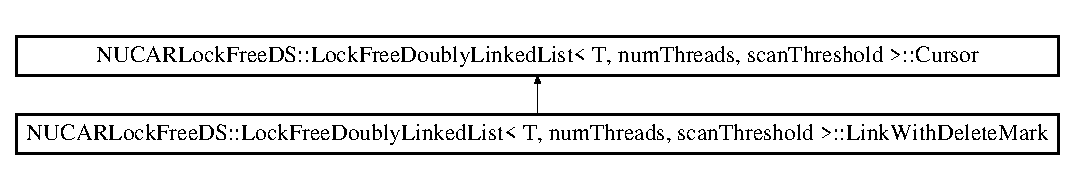
\includegraphics[height=1.839080cm]{class_n_u_c_a_r_lock_free_d_s_1_1_lock_free_doubly_linked_list_1_1_cursor}
\end{center}
\end{figure}


The documentation for this class was generated from the following file\+:\begin{DoxyCompactItemize}
\item 
G\+P\+U\+Lock\+Free\+Data\+Structures/\mbox{\hyperlink{_lock_free_doubly_linked_list_8hpp}{Lock\+Free\+Doubly\+Linked\+List.\+hpp}}\end{DoxyCompactItemize}

\hypertarget{class_n_u_c_a_r_lock_free_d_s_1_1_double_list_based_queue}{}\section{N\+U\+C\+A\+R\+Lock\+Free\+DS\+:\+:Double\+List\+Based\+Queue$<$ T, num\+Threads, scan\+Threshold $>$ Class Template Reference}
\label{class_n_u_c_a_r_lock_free_d_s_1_1_double_list_based_queue}\index{N\+U\+C\+A\+R\+Lock\+Free\+D\+S\+::\+Double\+List\+Based\+Queue$<$ T, num\+Threads, scan\+Threshold $>$@{N\+U\+C\+A\+R\+Lock\+Free\+D\+S\+::\+Double\+List\+Based\+Queue$<$ T, num\+Threads, scan\+Threshold $>$}}


{\ttfamily \#include $<$Double\+List\+Based\+Queue.\+hpp$>$}

\subsection*{Public Member Functions}
\begin{DoxyCompactItemize}
\item 
\+\_\+\+\_\+device\+\_\+\+\_\+ void \mbox{\hyperlink{class_n_u_c_a_r_lock_free_d_s_1_1_double_list_based_queue_ad9f196b3ea9ee4c684a5fab3c6bb9ddd}{enqueue}} (const T \&value)
\item 
\+\_\+\+\_\+device\+\_\+\+\_\+ bool \mbox{\hyperlink{class_n_u_c_a_r_lock_free_d_s_1_1_double_list_based_queue_a9541892be0892b41bc17a354586aa173}{dequeue}} (T \&result)
\end{DoxyCompactItemize}
\subsection*{Private Types}
\begin{DoxyCompactItemize}
\item 
using \mbox{\hyperlink{class_n_u_c_a_r_lock_free_d_s_1_1_double_list_based_queue_adfcec8aa40c6690e45107405c2fa2c35}{List\+\_\+t}} = \mbox{\hyperlink{class_n_u_c_a_r_lock_free_d_s_1_1_lock_free_doubly_linked_list}{Lock\+Free\+Doubly\+Linked\+List}}$<$ T, num\+Threads, scan\+Threshold $>$
\end{DoxyCompactItemize}
\subsection*{Private Attributes}
\begin{DoxyCompactItemize}
\item 
\mbox{\hyperlink{class_n_u_c_a_r_lock_free_d_s_1_1_double_list_based_queue_adfcec8aa40c6690e45107405c2fa2c35}{List\+\_\+t}} \mbox{\hyperlink{class_n_u_c_a_r_lock_free_d_s_1_1_double_list_based_queue_ac63ca28afaaf2cb487e9ff03b601e20b}{list}}
\end{DoxyCompactItemize}


\subsection{Member Typedef Documentation}
\mbox{\Hypertarget{class_n_u_c_a_r_lock_free_d_s_1_1_double_list_based_queue_adfcec8aa40c6690e45107405c2fa2c35}\label{class_n_u_c_a_r_lock_free_d_s_1_1_double_list_based_queue_adfcec8aa40c6690e45107405c2fa2c35}} 
\index{N\+U\+C\+A\+R\+Lock\+Free\+D\+S\+::\+Double\+List\+Based\+Queue@{N\+U\+C\+A\+R\+Lock\+Free\+D\+S\+::\+Double\+List\+Based\+Queue}!List\+\_\+t@{List\+\_\+t}}
\index{List\+\_\+t@{List\+\_\+t}!N\+U\+C\+A\+R\+Lock\+Free\+D\+S\+::\+Double\+List\+Based\+Queue@{N\+U\+C\+A\+R\+Lock\+Free\+D\+S\+::\+Double\+List\+Based\+Queue}}
\subsubsection{\texorpdfstring{List\+\_\+t}{List\_t}}
{\footnotesize\ttfamily template$<$typename T , Lock\+Free\+Doubly\+Linked\+List\+Config\+::\+Doubly\+Linked\+List\+Index\+\_\+t num\+Threads, Lock\+Free\+Doubly\+Linked\+List\+Config\+::\+Doubly\+Linked\+List\+Index\+\_\+t scan\+Threshold = Lock\+Free\+Doubly\+Linked\+List\+Config\+::\+Get\+Default\+Scan\+Threshold$<$\+Lock\+Free\+Doubly\+Linked\+List\+Config\+::\+Doubly\+Linked\+List\+Index\+\_\+t$>$(num\+Threads)$>$ \\
using \mbox{\hyperlink{class_n_u_c_a_r_lock_free_d_s_1_1_double_list_based_queue}{N\+U\+C\+A\+R\+Lock\+Free\+D\+S\+::\+Double\+List\+Based\+Queue}}$<$ T, num\+Threads, scan\+Threshold $>$\+::\mbox{\hyperlink{class_n_u_c_a_r_lock_free_d_s_1_1_double_list_based_queue_adfcec8aa40c6690e45107405c2fa2c35}{List\+\_\+t}} =  \mbox{\hyperlink{class_n_u_c_a_r_lock_free_d_s_1_1_lock_free_doubly_linked_list}{Lock\+Free\+Doubly\+Linked\+List}}$<$T, num\+Threads, scan\+Threshold$>$\hspace{0.3cm}{\ttfamily [private]}}



\subsection{Member Function Documentation}
\mbox{\Hypertarget{class_n_u_c_a_r_lock_free_d_s_1_1_double_list_based_queue_a9541892be0892b41bc17a354586aa173}\label{class_n_u_c_a_r_lock_free_d_s_1_1_double_list_based_queue_a9541892be0892b41bc17a354586aa173}} 
\index{N\+U\+C\+A\+R\+Lock\+Free\+D\+S\+::\+Double\+List\+Based\+Queue@{N\+U\+C\+A\+R\+Lock\+Free\+D\+S\+::\+Double\+List\+Based\+Queue}!dequeue@{dequeue}}
\index{dequeue@{dequeue}!N\+U\+C\+A\+R\+Lock\+Free\+D\+S\+::\+Double\+List\+Based\+Queue@{N\+U\+C\+A\+R\+Lock\+Free\+D\+S\+::\+Double\+List\+Based\+Queue}}
\subsubsection{\texorpdfstring{dequeue()}{dequeue()}}
{\footnotesize\ttfamily template$<$typename T , Lock\+Free\+Doubly\+Linked\+List\+Config\+::\+Doubly\+Linked\+List\+Index\+\_\+t num\+Threads, Lock\+Free\+Doubly\+Linked\+List\+Config\+::\+Doubly\+Linked\+List\+Index\+\_\+t scan\+Threshold = Lock\+Free\+Doubly\+Linked\+List\+Config\+::\+Get\+Default\+Scan\+Threshold$<$\+Lock\+Free\+Doubly\+Linked\+List\+Config\+::\+Doubly\+Linked\+List\+Index\+\_\+t$>$(num\+Threads)$>$ \\
\+\_\+\+\_\+device\+\_\+\+\_\+ bool \mbox{\hyperlink{class_n_u_c_a_r_lock_free_d_s_1_1_double_list_based_queue}{N\+U\+C\+A\+R\+Lock\+Free\+D\+S\+::\+Double\+List\+Based\+Queue}}$<$ T, num\+Threads, scan\+Threshold $>$\+::dequeue (\begin{DoxyParamCaption}\item[{T \&}]{result }\end{DoxyParamCaption})\hspace{0.3cm}{\ttfamily [inline]}}

\mbox{\Hypertarget{class_n_u_c_a_r_lock_free_d_s_1_1_double_list_based_queue_ad9f196b3ea9ee4c684a5fab3c6bb9ddd}\label{class_n_u_c_a_r_lock_free_d_s_1_1_double_list_based_queue_ad9f196b3ea9ee4c684a5fab3c6bb9ddd}} 
\index{N\+U\+C\+A\+R\+Lock\+Free\+D\+S\+::\+Double\+List\+Based\+Queue@{N\+U\+C\+A\+R\+Lock\+Free\+D\+S\+::\+Double\+List\+Based\+Queue}!enqueue@{enqueue}}
\index{enqueue@{enqueue}!N\+U\+C\+A\+R\+Lock\+Free\+D\+S\+::\+Double\+List\+Based\+Queue@{N\+U\+C\+A\+R\+Lock\+Free\+D\+S\+::\+Double\+List\+Based\+Queue}}
\subsubsection{\texorpdfstring{enqueue()}{enqueue()}}
{\footnotesize\ttfamily template$<$typename T , Lock\+Free\+Doubly\+Linked\+List\+Config\+::\+Doubly\+Linked\+List\+Index\+\_\+t num\+Threads, Lock\+Free\+Doubly\+Linked\+List\+Config\+::\+Doubly\+Linked\+List\+Index\+\_\+t scan\+Threshold = Lock\+Free\+Doubly\+Linked\+List\+Config\+::\+Get\+Default\+Scan\+Threshold$<$\+Lock\+Free\+Doubly\+Linked\+List\+Config\+::\+Doubly\+Linked\+List\+Index\+\_\+t$>$(num\+Threads)$>$ \\
\+\_\+\+\_\+device\+\_\+\+\_\+ void \mbox{\hyperlink{class_n_u_c_a_r_lock_free_d_s_1_1_double_list_based_queue}{N\+U\+C\+A\+R\+Lock\+Free\+D\+S\+::\+Double\+List\+Based\+Queue}}$<$ T, num\+Threads, scan\+Threshold $>$\+::enqueue (\begin{DoxyParamCaption}\item[{const T \&}]{value }\end{DoxyParamCaption})\hspace{0.3cm}{\ttfamily [inline]}}



\subsection{Member Data Documentation}
\mbox{\Hypertarget{class_n_u_c_a_r_lock_free_d_s_1_1_double_list_based_queue_ac63ca28afaaf2cb487e9ff03b601e20b}\label{class_n_u_c_a_r_lock_free_d_s_1_1_double_list_based_queue_ac63ca28afaaf2cb487e9ff03b601e20b}} 
\index{N\+U\+C\+A\+R\+Lock\+Free\+D\+S\+::\+Double\+List\+Based\+Queue@{N\+U\+C\+A\+R\+Lock\+Free\+D\+S\+::\+Double\+List\+Based\+Queue}!list@{list}}
\index{list@{list}!N\+U\+C\+A\+R\+Lock\+Free\+D\+S\+::\+Double\+List\+Based\+Queue@{N\+U\+C\+A\+R\+Lock\+Free\+D\+S\+::\+Double\+List\+Based\+Queue}}
\subsubsection{\texorpdfstring{list}{list}}
{\footnotesize\ttfamily template$<$typename T , Lock\+Free\+Doubly\+Linked\+List\+Config\+::\+Doubly\+Linked\+List\+Index\+\_\+t num\+Threads, Lock\+Free\+Doubly\+Linked\+List\+Config\+::\+Doubly\+Linked\+List\+Index\+\_\+t scan\+Threshold = Lock\+Free\+Doubly\+Linked\+List\+Config\+::\+Get\+Default\+Scan\+Threshold$<$\+Lock\+Free\+Doubly\+Linked\+List\+Config\+::\+Doubly\+Linked\+List\+Index\+\_\+t$>$(num\+Threads)$>$ \\
\mbox{\hyperlink{class_n_u_c_a_r_lock_free_d_s_1_1_double_list_based_queue_adfcec8aa40c6690e45107405c2fa2c35}{List\+\_\+t}} \mbox{\hyperlink{class_n_u_c_a_r_lock_free_d_s_1_1_double_list_based_queue}{N\+U\+C\+A\+R\+Lock\+Free\+D\+S\+::\+Double\+List\+Based\+Queue}}$<$ T, num\+Threads, scan\+Threshold $>$\+::list\hspace{0.3cm}{\ttfamily [private]}}



The documentation for this class was generated from the following file\+:\begin{DoxyCompactItemize}
\item 
G\+P\+U\+Lock\+Free\+Data\+Structures/\mbox{\hyperlink{_double_list_based_queue_8hpp}{Double\+List\+Based\+Queue.\+hpp}}\end{DoxyCompactItemize}

\hypertarget{class_n_u_c_a_r_lock_free_d_s_1_1_double_list_based_stack}{}\section{N\+U\+C\+A\+R\+Lock\+Free\+DS\+:\+:Double\+List\+Based\+Stack$<$ T, num\+Threads, scan\+Threshold $>$ Class Template Reference}
\label{class_n_u_c_a_r_lock_free_d_s_1_1_double_list_based_stack}\index{N\+U\+C\+A\+R\+Lock\+Free\+D\+S\+::\+Double\+List\+Based\+Stack$<$ T, num\+Threads, scan\+Threshold $>$@{N\+U\+C\+A\+R\+Lock\+Free\+D\+S\+::\+Double\+List\+Based\+Stack$<$ T, num\+Threads, scan\+Threshold $>$}}


{\ttfamily \#include $<$Double\+List\+Based\+Stack.\+hpp$>$}

\subsection*{Public Member Functions}
\begin{DoxyCompactItemize}
\item 
\+\_\+\+\_\+device\+\_\+\+\_\+ void \mbox{\hyperlink{class_n_u_c_a_r_lock_free_d_s_1_1_double_list_based_stack_aa7be3345eca6fad8f568c3a1b9bf1fd6}{push}} (const T \&value)
\item 
\+\_\+\+\_\+device\+\_\+\+\_\+ bool \mbox{\hyperlink{class_n_u_c_a_r_lock_free_d_s_1_1_double_list_based_stack_a5ff2af6c3939738c9a225107242467c9}{pop}} (T \&result)
\end{DoxyCompactItemize}
\subsection*{Private Types}
\begin{DoxyCompactItemize}
\item 
using \mbox{\hyperlink{class_n_u_c_a_r_lock_free_d_s_1_1_double_list_based_stack_a1ef386e8aaa2b4bb17d44df51f0c9f76}{List\+\_\+t}} = \mbox{\hyperlink{class_n_u_c_a_r_lock_free_d_s_1_1_lock_free_doubly_linked_list}{Lock\+Free\+Doubly\+Linked\+List}}$<$ T, num\+Threads, scan\+Threshold $>$
\end{DoxyCompactItemize}
\subsection*{Private Attributes}
\begin{DoxyCompactItemize}
\item 
\mbox{\hyperlink{class_n_u_c_a_r_lock_free_d_s_1_1_double_list_based_stack_a1ef386e8aaa2b4bb17d44df51f0c9f76}{List\+\_\+t}} \mbox{\hyperlink{class_n_u_c_a_r_lock_free_d_s_1_1_double_list_based_stack_abc2cb5a9e08f892c83fd811506eddc05}{list}}
\end{DoxyCompactItemize}


\subsection{Member Typedef Documentation}
\mbox{\Hypertarget{class_n_u_c_a_r_lock_free_d_s_1_1_double_list_based_stack_a1ef386e8aaa2b4bb17d44df51f0c9f76}\label{class_n_u_c_a_r_lock_free_d_s_1_1_double_list_based_stack_a1ef386e8aaa2b4bb17d44df51f0c9f76}} 
\index{N\+U\+C\+A\+R\+Lock\+Free\+D\+S\+::\+Double\+List\+Based\+Stack@{N\+U\+C\+A\+R\+Lock\+Free\+D\+S\+::\+Double\+List\+Based\+Stack}!List\+\_\+t@{List\+\_\+t}}
\index{List\+\_\+t@{List\+\_\+t}!N\+U\+C\+A\+R\+Lock\+Free\+D\+S\+::\+Double\+List\+Based\+Stack@{N\+U\+C\+A\+R\+Lock\+Free\+D\+S\+::\+Double\+List\+Based\+Stack}}
\subsubsection{\texorpdfstring{List\+\_\+t}{List\_t}}
{\footnotesize\ttfamily template$<$typename T , Lock\+Free\+Doubly\+Linked\+List\+Config\+::\+Doubly\+Linked\+List\+Index\+\_\+t num\+Threads, Lock\+Free\+Doubly\+Linked\+List\+Config\+::\+Doubly\+Linked\+List\+Index\+\_\+t scan\+Threshold = Lock\+Free\+Doubly\+Linked\+List\+Config\+::\+Get\+Default\+Scan\+Threshold$<$\+Lock\+Free\+Doubly\+Linked\+List\+Config\+::\+Doubly\+Linked\+List\+Index\+\_\+t$>$(num\+Threads)$>$ \\
using \mbox{\hyperlink{class_n_u_c_a_r_lock_free_d_s_1_1_double_list_based_stack}{N\+U\+C\+A\+R\+Lock\+Free\+D\+S\+::\+Double\+List\+Based\+Stack}}$<$ T, num\+Threads, scan\+Threshold $>$\+::\mbox{\hyperlink{class_n_u_c_a_r_lock_free_d_s_1_1_double_list_based_stack_a1ef386e8aaa2b4bb17d44df51f0c9f76}{List\+\_\+t}} =  \mbox{\hyperlink{class_n_u_c_a_r_lock_free_d_s_1_1_lock_free_doubly_linked_list}{Lock\+Free\+Doubly\+Linked\+List}}$<$T, num\+Threads, scan\+Threshold$>$\hspace{0.3cm}{\ttfamily [private]}}



\subsection{Member Function Documentation}
\mbox{\Hypertarget{class_n_u_c_a_r_lock_free_d_s_1_1_double_list_based_stack_a5ff2af6c3939738c9a225107242467c9}\label{class_n_u_c_a_r_lock_free_d_s_1_1_double_list_based_stack_a5ff2af6c3939738c9a225107242467c9}} 
\index{N\+U\+C\+A\+R\+Lock\+Free\+D\+S\+::\+Double\+List\+Based\+Stack@{N\+U\+C\+A\+R\+Lock\+Free\+D\+S\+::\+Double\+List\+Based\+Stack}!pop@{pop}}
\index{pop@{pop}!N\+U\+C\+A\+R\+Lock\+Free\+D\+S\+::\+Double\+List\+Based\+Stack@{N\+U\+C\+A\+R\+Lock\+Free\+D\+S\+::\+Double\+List\+Based\+Stack}}
\subsubsection{\texorpdfstring{pop()}{pop()}}
{\footnotesize\ttfamily template$<$typename T , Lock\+Free\+Doubly\+Linked\+List\+Config\+::\+Doubly\+Linked\+List\+Index\+\_\+t num\+Threads, Lock\+Free\+Doubly\+Linked\+List\+Config\+::\+Doubly\+Linked\+List\+Index\+\_\+t scan\+Threshold = Lock\+Free\+Doubly\+Linked\+List\+Config\+::\+Get\+Default\+Scan\+Threshold$<$\+Lock\+Free\+Doubly\+Linked\+List\+Config\+::\+Doubly\+Linked\+List\+Index\+\_\+t$>$(num\+Threads)$>$ \\
\+\_\+\+\_\+device\+\_\+\+\_\+ bool \mbox{\hyperlink{class_n_u_c_a_r_lock_free_d_s_1_1_double_list_based_stack}{N\+U\+C\+A\+R\+Lock\+Free\+D\+S\+::\+Double\+List\+Based\+Stack}}$<$ T, num\+Threads, scan\+Threshold $>$\+::pop (\begin{DoxyParamCaption}\item[{T \&}]{result }\end{DoxyParamCaption})\hspace{0.3cm}{\ttfamily [inline]}}

\mbox{\Hypertarget{class_n_u_c_a_r_lock_free_d_s_1_1_double_list_based_stack_aa7be3345eca6fad8f568c3a1b9bf1fd6}\label{class_n_u_c_a_r_lock_free_d_s_1_1_double_list_based_stack_aa7be3345eca6fad8f568c3a1b9bf1fd6}} 
\index{N\+U\+C\+A\+R\+Lock\+Free\+D\+S\+::\+Double\+List\+Based\+Stack@{N\+U\+C\+A\+R\+Lock\+Free\+D\+S\+::\+Double\+List\+Based\+Stack}!push@{push}}
\index{push@{push}!N\+U\+C\+A\+R\+Lock\+Free\+D\+S\+::\+Double\+List\+Based\+Stack@{N\+U\+C\+A\+R\+Lock\+Free\+D\+S\+::\+Double\+List\+Based\+Stack}}
\subsubsection{\texorpdfstring{push()}{push()}}
{\footnotesize\ttfamily template$<$typename T , Lock\+Free\+Doubly\+Linked\+List\+Config\+::\+Doubly\+Linked\+List\+Index\+\_\+t num\+Threads, Lock\+Free\+Doubly\+Linked\+List\+Config\+::\+Doubly\+Linked\+List\+Index\+\_\+t scan\+Threshold = Lock\+Free\+Doubly\+Linked\+List\+Config\+::\+Get\+Default\+Scan\+Threshold$<$\+Lock\+Free\+Doubly\+Linked\+List\+Config\+::\+Doubly\+Linked\+List\+Index\+\_\+t$>$(num\+Threads)$>$ \\
\+\_\+\+\_\+device\+\_\+\+\_\+ void \mbox{\hyperlink{class_n_u_c_a_r_lock_free_d_s_1_1_double_list_based_stack}{N\+U\+C\+A\+R\+Lock\+Free\+D\+S\+::\+Double\+List\+Based\+Stack}}$<$ T, num\+Threads, scan\+Threshold $>$\+::push (\begin{DoxyParamCaption}\item[{const T \&}]{value }\end{DoxyParamCaption})\hspace{0.3cm}{\ttfamily [inline]}}



\subsection{Member Data Documentation}
\mbox{\Hypertarget{class_n_u_c_a_r_lock_free_d_s_1_1_double_list_based_stack_abc2cb5a9e08f892c83fd811506eddc05}\label{class_n_u_c_a_r_lock_free_d_s_1_1_double_list_based_stack_abc2cb5a9e08f892c83fd811506eddc05}} 
\index{N\+U\+C\+A\+R\+Lock\+Free\+D\+S\+::\+Double\+List\+Based\+Stack@{N\+U\+C\+A\+R\+Lock\+Free\+D\+S\+::\+Double\+List\+Based\+Stack}!list@{list}}
\index{list@{list}!N\+U\+C\+A\+R\+Lock\+Free\+D\+S\+::\+Double\+List\+Based\+Stack@{N\+U\+C\+A\+R\+Lock\+Free\+D\+S\+::\+Double\+List\+Based\+Stack}}
\subsubsection{\texorpdfstring{list}{list}}
{\footnotesize\ttfamily template$<$typename T , Lock\+Free\+Doubly\+Linked\+List\+Config\+::\+Doubly\+Linked\+List\+Index\+\_\+t num\+Threads, Lock\+Free\+Doubly\+Linked\+List\+Config\+::\+Doubly\+Linked\+List\+Index\+\_\+t scan\+Threshold = Lock\+Free\+Doubly\+Linked\+List\+Config\+::\+Get\+Default\+Scan\+Threshold$<$\+Lock\+Free\+Doubly\+Linked\+List\+Config\+::\+Doubly\+Linked\+List\+Index\+\_\+t$>$(num\+Threads)$>$ \\
\mbox{\hyperlink{class_n_u_c_a_r_lock_free_d_s_1_1_double_list_based_stack_a1ef386e8aaa2b4bb17d44df51f0c9f76}{List\+\_\+t}} \mbox{\hyperlink{class_n_u_c_a_r_lock_free_d_s_1_1_double_list_based_stack}{N\+U\+C\+A\+R\+Lock\+Free\+D\+S\+::\+Double\+List\+Based\+Stack}}$<$ T, num\+Threads, scan\+Threshold $>$\+::list\hspace{0.3cm}{\ttfamily [private]}}



The documentation for this class was generated from the following file\+:\begin{DoxyCompactItemize}
\item 
G\+P\+U\+Lock\+Free\+Data\+Structures/\mbox{\hyperlink{_double_list_based_stack_8hpp}{Double\+List\+Based\+Stack.\+hpp}}\end{DoxyCompactItemize}

\hypertarget{class_n_u_c_a_r_lock_free_d_s_1_1_lock_free_doubly_linked_list_1_1_linked_list_node}{}\section{N\+U\+C\+A\+R\+Lock\+Free\+DS\+:\+:Lock\+Free\+Doubly\+Linked\+List$<$ T, num\+Threads, scan\+Threshold $>$\+:\+:Linked\+List\+Node Class Reference}
\label{class_n_u_c_a_r_lock_free_d_s_1_1_lock_free_doubly_linked_list_1_1_linked_list_node}\index{N\+U\+C\+A\+R\+Lock\+Free\+D\+S\+::\+Lock\+Free\+Doubly\+Linked\+List$<$ T, num\+Threads, scan\+Threshold $>$\+::\+Linked\+List\+Node@{N\+U\+C\+A\+R\+Lock\+Free\+D\+S\+::\+Lock\+Free\+Doubly\+Linked\+List$<$ T, num\+Threads, scan\+Threshold $>$\+::\+Linked\+List\+Node}}
\subsection*{Public Member Functions}
\begin{DoxyCompactItemize}
\item 
\+\_\+\+\_\+device\+\_\+\+\_\+ \mbox{\hyperlink{class_n_u_c_a_r_lock_free_d_s_1_1_lock_free_doubly_linked_list_1_1_linked_list_node_a47208e6922870bba81cbd7c59265b4b4}{Linked\+List\+Node}} ()
\item 
\+\_\+\+\_\+device\+\_\+\+\_\+ \mbox{\hyperlink{class_n_u_c_a_r_lock_free_d_s_1_1_lock_free_doubly_linked_list_a08f21d5e04bc2a02d6c1d8861a6ba0de}{Link\+\_\+t}} $\ast$ \mbox{\hyperlink{class_n_u_c_a_r_lock_free_d_s_1_1_lock_free_doubly_linked_list_1_1_linked_list_node_ae1a75bbfaccfe1d566803fbeb2298679}{get\+PrevP}} ()
\item 
\+\_\+\+\_\+device\+\_\+\+\_\+ \mbox{\hyperlink{class_n_u_c_a_r_lock_free_d_s_1_1_lock_free_doubly_linked_list_a08f21d5e04bc2a02d6c1d8861a6ba0de}{Link\+\_\+t}} $\ast$ \mbox{\hyperlink{class_n_u_c_a_r_lock_free_d_s_1_1_lock_free_doubly_linked_list_1_1_linked_list_node_ae06fa31bdcd570875cd83af2c78bdd3b}{get\+NextP}} ()
\item 
\+\_\+\+\_\+device\+\_\+\+\_\+ \mbox{\hyperlink{class_n_u_c_a_r_lock_free_d_s_1_1_lock_free_doubly_linked_list_a08f21d5e04bc2a02d6c1d8861a6ba0de}{Link\+\_\+t}} \mbox{\hyperlink{class_n_u_c_a_r_lock_free_d_s_1_1_lock_free_doubly_linked_list_1_1_linked_list_node_ae5bc375f39c02a40709a9ada2469ca66}{atomic\+Read\+Prev}} ()
\item 
\+\_\+\+\_\+device\+\_\+\+\_\+ \mbox{\hyperlink{class_n_u_c_a_r_lock_free_d_s_1_1_lock_free_doubly_linked_list_a08f21d5e04bc2a02d6c1d8861a6ba0de}{Link\+\_\+t}} \mbox{\hyperlink{class_n_u_c_a_r_lock_free_d_s_1_1_lock_free_doubly_linked_list_1_1_linked_list_node_aaba42c339b0a5dc28eb40fca182e104a}{atomic\+Read\+Next}} ()
\end{DoxyCompactItemize}
\subsection*{Public Attributes}
\begin{DoxyCompactItemize}
\item 
T \mbox{\hyperlink{class_n_u_c_a_r_lock_free_d_s_1_1_lock_free_doubly_linked_list_1_1_linked_list_node_ae9136b50ed0477d43e6b6707b90c14c1}{value}}
\end{DoxyCompactItemize}
\subsection*{Private Attributes}
\begin{DoxyCompactItemize}
\item 
\mbox{\hyperlink{class_n_u_c_a_r_lock_free_d_s_1_1_lock_free_doubly_linked_list_a08f21d5e04bc2a02d6c1d8861a6ba0de}{Link\+\_\+t}} \mbox{\hyperlink{class_n_u_c_a_r_lock_free_d_s_1_1_lock_free_doubly_linked_list_1_1_linked_list_node_ae9d1647c3b7780a17ba51454410263d4}{prev}}
\item 
\mbox{\hyperlink{class_n_u_c_a_r_lock_free_d_s_1_1_lock_free_doubly_linked_list_a08f21d5e04bc2a02d6c1d8861a6ba0de}{Link\+\_\+t}} \mbox{\hyperlink{class_n_u_c_a_r_lock_free_d_s_1_1_lock_free_doubly_linked_list_1_1_linked_list_node_a332a3dae6b1138e2283734792c85a97c}{next}}
\end{DoxyCompactItemize}


\subsection{Constructor \& Destructor Documentation}
\mbox{\Hypertarget{class_n_u_c_a_r_lock_free_d_s_1_1_lock_free_doubly_linked_list_1_1_linked_list_node_a47208e6922870bba81cbd7c59265b4b4}\label{class_n_u_c_a_r_lock_free_d_s_1_1_lock_free_doubly_linked_list_1_1_linked_list_node_a47208e6922870bba81cbd7c59265b4b4}} 
\index{N\+U\+C\+A\+R\+Lock\+Free\+D\+S\+::\+Lock\+Free\+Doubly\+Linked\+List\+::\+Linked\+List\+Node@{N\+U\+C\+A\+R\+Lock\+Free\+D\+S\+::\+Lock\+Free\+Doubly\+Linked\+List\+::\+Linked\+List\+Node}!Linked\+List\+Node@{Linked\+List\+Node}}
\index{Linked\+List\+Node@{Linked\+List\+Node}!N\+U\+C\+A\+R\+Lock\+Free\+D\+S\+::\+Lock\+Free\+Doubly\+Linked\+List\+::\+Linked\+List\+Node@{N\+U\+C\+A\+R\+Lock\+Free\+D\+S\+::\+Lock\+Free\+Doubly\+Linked\+List\+::\+Linked\+List\+Node}}
\subsubsection{\texorpdfstring{Linked\+List\+Node()}{LinkedListNode()}}
{\footnotesize\ttfamily template$<$typename T , Lock\+Free\+Doubly\+Linked\+List\+Config\+::\+Doubly\+Linked\+List\+Index\+\_\+t num\+Threads, Lock\+Free\+Doubly\+Linked\+List\+Config\+::\+Doubly\+Linked\+List\+Index\+\_\+t scan\+Threshold = Lock\+Free\+Doubly\+Linked\+List\+Config\+::\+Get\+Default\+Scan\+Threshold$<$\+Lock\+Free\+Doubly\+Linked\+List\+Config\+::\+Doubly\+Linked\+List\+Index\+\_\+t$>$(num\+Threads)$>$ \\
\+\_\+\+\_\+device\+\_\+\+\_\+ \mbox{\hyperlink{class_n_u_c_a_r_lock_free_d_s_1_1_lock_free_doubly_linked_list}{N\+U\+C\+A\+R\+Lock\+Free\+D\+S\+::\+Lock\+Free\+Doubly\+Linked\+List}}$<$ T, num\+Threads, scan\+Threshold $>$\+::Linked\+List\+Node\+::\+Linked\+List\+Node (\begin{DoxyParamCaption}{ }\end{DoxyParamCaption})\hspace{0.3cm}{\ttfamily [inline]}}



\subsection{Member Function Documentation}
\mbox{\Hypertarget{class_n_u_c_a_r_lock_free_d_s_1_1_lock_free_doubly_linked_list_1_1_linked_list_node_aaba42c339b0a5dc28eb40fca182e104a}\label{class_n_u_c_a_r_lock_free_d_s_1_1_lock_free_doubly_linked_list_1_1_linked_list_node_aaba42c339b0a5dc28eb40fca182e104a}} 
\index{N\+U\+C\+A\+R\+Lock\+Free\+D\+S\+::\+Lock\+Free\+Doubly\+Linked\+List\+::\+Linked\+List\+Node@{N\+U\+C\+A\+R\+Lock\+Free\+D\+S\+::\+Lock\+Free\+Doubly\+Linked\+List\+::\+Linked\+List\+Node}!atomic\+Read\+Next@{atomic\+Read\+Next}}
\index{atomic\+Read\+Next@{atomic\+Read\+Next}!N\+U\+C\+A\+R\+Lock\+Free\+D\+S\+::\+Lock\+Free\+Doubly\+Linked\+List\+::\+Linked\+List\+Node@{N\+U\+C\+A\+R\+Lock\+Free\+D\+S\+::\+Lock\+Free\+Doubly\+Linked\+List\+::\+Linked\+List\+Node}}
\subsubsection{\texorpdfstring{atomic\+Read\+Next()}{atomicReadNext()}}
{\footnotesize\ttfamily template$<$typename T , Lock\+Free\+Doubly\+Linked\+List\+Config\+::\+Doubly\+Linked\+List\+Index\+\_\+t num\+Threads, Lock\+Free\+Doubly\+Linked\+List\+Config\+::\+Doubly\+Linked\+List\+Index\+\_\+t scan\+Threshold = Lock\+Free\+Doubly\+Linked\+List\+Config\+::\+Get\+Default\+Scan\+Threshold$<$\+Lock\+Free\+Doubly\+Linked\+List\+Config\+::\+Doubly\+Linked\+List\+Index\+\_\+t$>$(num\+Threads)$>$ \\
\+\_\+\+\_\+device\+\_\+\+\_\+ \mbox{\hyperlink{class_n_u_c_a_r_lock_free_d_s_1_1_lock_free_doubly_linked_list_a08f21d5e04bc2a02d6c1d8861a6ba0de}{Link\+\_\+t}} \mbox{\hyperlink{class_n_u_c_a_r_lock_free_d_s_1_1_lock_free_doubly_linked_list}{N\+U\+C\+A\+R\+Lock\+Free\+D\+S\+::\+Lock\+Free\+Doubly\+Linked\+List}}$<$ T, num\+Threads, scan\+Threshold $>$\+::Linked\+List\+Node\+::atomic\+Read\+Next (\begin{DoxyParamCaption}{ }\end{DoxyParamCaption})\hspace{0.3cm}{\ttfamily [inline]}}

\mbox{\Hypertarget{class_n_u_c_a_r_lock_free_d_s_1_1_lock_free_doubly_linked_list_1_1_linked_list_node_ae5bc375f39c02a40709a9ada2469ca66}\label{class_n_u_c_a_r_lock_free_d_s_1_1_lock_free_doubly_linked_list_1_1_linked_list_node_ae5bc375f39c02a40709a9ada2469ca66}} 
\index{N\+U\+C\+A\+R\+Lock\+Free\+D\+S\+::\+Lock\+Free\+Doubly\+Linked\+List\+::\+Linked\+List\+Node@{N\+U\+C\+A\+R\+Lock\+Free\+D\+S\+::\+Lock\+Free\+Doubly\+Linked\+List\+::\+Linked\+List\+Node}!atomic\+Read\+Prev@{atomic\+Read\+Prev}}
\index{atomic\+Read\+Prev@{atomic\+Read\+Prev}!N\+U\+C\+A\+R\+Lock\+Free\+D\+S\+::\+Lock\+Free\+Doubly\+Linked\+List\+::\+Linked\+List\+Node@{N\+U\+C\+A\+R\+Lock\+Free\+D\+S\+::\+Lock\+Free\+Doubly\+Linked\+List\+::\+Linked\+List\+Node}}
\subsubsection{\texorpdfstring{atomic\+Read\+Prev()}{atomicReadPrev()}}
{\footnotesize\ttfamily template$<$typename T , Lock\+Free\+Doubly\+Linked\+List\+Config\+::\+Doubly\+Linked\+List\+Index\+\_\+t num\+Threads, Lock\+Free\+Doubly\+Linked\+List\+Config\+::\+Doubly\+Linked\+List\+Index\+\_\+t scan\+Threshold = Lock\+Free\+Doubly\+Linked\+List\+Config\+::\+Get\+Default\+Scan\+Threshold$<$\+Lock\+Free\+Doubly\+Linked\+List\+Config\+::\+Doubly\+Linked\+List\+Index\+\_\+t$>$(num\+Threads)$>$ \\
\+\_\+\+\_\+device\+\_\+\+\_\+ \mbox{\hyperlink{class_n_u_c_a_r_lock_free_d_s_1_1_lock_free_doubly_linked_list_a08f21d5e04bc2a02d6c1d8861a6ba0de}{Link\+\_\+t}} \mbox{\hyperlink{class_n_u_c_a_r_lock_free_d_s_1_1_lock_free_doubly_linked_list}{N\+U\+C\+A\+R\+Lock\+Free\+D\+S\+::\+Lock\+Free\+Doubly\+Linked\+List}}$<$ T, num\+Threads, scan\+Threshold $>$\+::Linked\+List\+Node\+::atomic\+Read\+Prev (\begin{DoxyParamCaption}{ }\end{DoxyParamCaption})\hspace{0.3cm}{\ttfamily [inline]}}

\mbox{\Hypertarget{class_n_u_c_a_r_lock_free_d_s_1_1_lock_free_doubly_linked_list_1_1_linked_list_node_ae06fa31bdcd570875cd83af2c78bdd3b}\label{class_n_u_c_a_r_lock_free_d_s_1_1_lock_free_doubly_linked_list_1_1_linked_list_node_ae06fa31bdcd570875cd83af2c78bdd3b}} 
\index{N\+U\+C\+A\+R\+Lock\+Free\+D\+S\+::\+Lock\+Free\+Doubly\+Linked\+List\+::\+Linked\+List\+Node@{N\+U\+C\+A\+R\+Lock\+Free\+D\+S\+::\+Lock\+Free\+Doubly\+Linked\+List\+::\+Linked\+List\+Node}!get\+NextP@{get\+NextP}}
\index{get\+NextP@{get\+NextP}!N\+U\+C\+A\+R\+Lock\+Free\+D\+S\+::\+Lock\+Free\+Doubly\+Linked\+List\+::\+Linked\+List\+Node@{N\+U\+C\+A\+R\+Lock\+Free\+D\+S\+::\+Lock\+Free\+Doubly\+Linked\+List\+::\+Linked\+List\+Node}}
\subsubsection{\texorpdfstring{get\+Next\+P()}{getNextP()}}
{\footnotesize\ttfamily template$<$typename T , Lock\+Free\+Doubly\+Linked\+List\+Config\+::\+Doubly\+Linked\+List\+Index\+\_\+t num\+Threads, Lock\+Free\+Doubly\+Linked\+List\+Config\+::\+Doubly\+Linked\+List\+Index\+\_\+t scan\+Threshold = Lock\+Free\+Doubly\+Linked\+List\+Config\+::\+Get\+Default\+Scan\+Threshold$<$\+Lock\+Free\+Doubly\+Linked\+List\+Config\+::\+Doubly\+Linked\+List\+Index\+\_\+t$>$(num\+Threads)$>$ \\
\+\_\+\+\_\+device\+\_\+\+\_\+ \mbox{\hyperlink{class_n_u_c_a_r_lock_free_d_s_1_1_lock_free_doubly_linked_list_a08f21d5e04bc2a02d6c1d8861a6ba0de}{Link\+\_\+t}}$\ast$ \mbox{\hyperlink{class_n_u_c_a_r_lock_free_d_s_1_1_lock_free_doubly_linked_list}{N\+U\+C\+A\+R\+Lock\+Free\+D\+S\+::\+Lock\+Free\+Doubly\+Linked\+List}}$<$ T, num\+Threads, scan\+Threshold $>$\+::Linked\+List\+Node\+::get\+NextP (\begin{DoxyParamCaption}{ }\end{DoxyParamCaption})\hspace{0.3cm}{\ttfamily [inline]}}

\mbox{\Hypertarget{class_n_u_c_a_r_lock_free_d_s_1_1_lock_free_doubly_linked_list_1_1_linked_list_node_ae1a75bbfaccfe1d566803fbeb2298679}\label{class_n_u_c_a_r_lock_free_d_s_1_1_lock_free_doubly_linked_list_1_1_linked_list_node_ae1a75bbfaccfe1d566803fbeb2298679}} 
\index{N\+U\+C\+A\+R\+Lock\+Free\+D\+S\+::\+Lock\+Free\+Doubly\+Linked\+List\+::\+Linked\+List\+Node@{N\+U\+C\+A\+R\+Lock\+Free\+D\+S\+::\+Lock\+Free\+Doubly\+Linked\+List\+::\+Linked\+List\+Node}!get\+PrevP@{get\+PrevP}}
\index{get\+PrevP@{get\+PrevP}!N\+U\+C\+A\+R\+Lock\+Free\+D\+S\+::\+Lock\+Free\+Doubly\+Linked\+List\+::\+Linked\+List\+Node@{N\+U\+C\+A\+R\+Lock\+Free\+D\+S\+::\+Lock\+Free\+Doubly\+Linked\+List\+::\+Linked\+List\+Node}}
\subsubsection{\texorpdfstring{get\+Prev\+P()}{getPrevP()}}
{\footnotesize\ttfamily template$<$typename T , Lock\+Free\+Doubly\+Linked\+List\+Config\+::\+Doubly\+Linked\+List\+Index\+\_\+t num\+Threads, Lock\+Free\+Doubly\+Linked\+List\+Config\+::\+Doubly\+Linked\+List\+Index\+\_\+t scan\+Threshold = Lock\+Free\+Doubly\+Linked\+List\+Config\+::\+Get\+Default\+Scan\+Threshold$<$\+Lock\+Free\+Doubly\+Linked\+List\+Config\+::\+Doubly\+Linked\+List\+Index\+\_\+t$>$(num\+Threads)$>$ \\
\+\_\+\+\_\+device\+\_\+\+\_\+ \mbox{\hyperlink{class_n_u_c_a_r_lock_free_d_s_1_1_lock_free_doubly_linked_list_a08f21d5e04bc2a02d6c1d8861a6ba0de}{Link\+\_\+t}}$\ast$ \mbox{\hyperlink{class_n_u_c_a_r_lock_free_d_s_1_1_lock_free_doubly_linked_list}{N\+U\+C\+A\+R\+Lock\+Free\+D\+S\+::\+Lock\+Free\+Doubly\+Linked\+List}}$<$ T, num\+Threads, scan\+Threshold $>$\+::Linked\+List\+Node\+::get\+PrevP (\begin{DoxyParamCaption}{ }\end{DoxyParamCaption})\hspace{0.3cm}{\ttfamily [inline]}}



\subsection{Member Data Documentation}
\mbox{\Hypertarget{class_n_u_c_a_r_lock_free_d_s_1_1_lock_free_doubly_linked_list_1_1_linked_list_node_a332a3dae6b1138e2283734792c85a97c}\label{class_n_u_c_a_r_lock_free_d_s_1_1_lock_free_doubly_linked_list_1_1_linked_list_node_a332a3dae6b1138e2283734792c85a97c}} 
\index{N\+U\+C\+A\+R\+Lock\+Free\+D\+S\+::\+Lock\+Free\+Doubly\+Linked\+List\+::\+Linked\+List\+Node@{N\+U\+C\+A\+R\+Lock\+Free\+D\+S\+::\+Lock\+Free\+Doubly\+Linked\+List\+::\+Linked\+List\+Node}!next@{next}}
\index{next@{next}!N\+U\+C\+A\+R\+Lock\+Free\+D\+S\+::\+Lock\+Free\+Doubly\+Linked\+List\+::\+Linked\+List\+Node@{N\+U\+C\+A\+R\+Lock\+Free\+D\+S\+::\+Lock\+Free\+Doubly\+Linked\+List\+::\+Linked\+List\+Node}}
\subsubsection{\texorpdfstring{next}{next}}
{\footnotesize\ttfamily template$<$typename T , Lock\+Free\+Doubly\+Linked\+List\+Config\+::\+Doubly\+Linked\+List\+Index\+\_\+t num\+Threads, Lock\+Free\+Doubly\+Linked\+List\+Config\+::\+Doubly\+Linked\+List\+Index\+\_\+t scan\+Threshold = Lock\+Free\+Doubly\+Linked\+List\+Config\+::\+Get\+Default\+Scan\+Threshold$<$\+Lock\+Free\+Doubly\+Linked\+List\+Config\+::\+Doubly\+Linked\+List\+Index\+\_\+t$>$(num\+Threads)$>$ \\
\mbox{\hyperlink{class_n_u_c_a_r_lock_free_d_s_1_1_lock_free_doubly_linked_list_a08f21d5e04bc2a02d6c1d8861a6ba0de}{Link\+\_\+t}} \mbox{\hyperlink{class_n_u_c_a_r_lock_free_d_s_1_1_lock_free_doubly_linked_list}{N\+U\+C\+A\+R\+Lock\+Free\+D\+S\+::\+Lock\+Free\+Doubly\+Linked\+List}}$<$ T, num\+Threads, scan\+Threshold $>$\+::Linked\+List\+Node\+::next\hspace{0.3cm}{\ttfamily [private]}}

\mbox{\Hypertarget{class_n_u_c_a_r_lock_free_d_s_1_1_lock_free_doubly_linked_list_1_1_linked_list_node_ae9d1647c3b7780a17ba51454410263d4}\label{class_n_u_c_a_r_lock_free_d_s_1_1_lock_free_doubly_linked_list_1_1_linked_list_node_ae9d1647c3b7780a17ba51454410263d4}} 
\index{N\+U\+C\+A\+R\+Lock\+Free\+D\+S\+::\+Lock\+Free\+Doubly\+Linked\+List\+::\+Linked\+List\+Node@{N\+U\+C\+A\+R\+Lock\+Free\+D\+S\+::\+Lock\+Free\+Doubly\+Linked\+List\+::\+Linked\+List\+Node}!prev@{prev}}
\index{prev@{prev}!N\+U\+C\+A\+R\+Lock\+Free\+D\+S\+::\+Lock\+Free\+Doubly\+Linked\+List\+::\+Linked\+List\+Node@{N\+U\+C\+A\+R\+Lock\+Free\+D\+S\+::\+Lock\+Free\+Doubly\+Linked\+List\+::\+Linked\+List\+Node}}
\subsubsection{\texorpdfstring{prev}{prev}}
{\footnotesize\ttfamily template$<$typename T , Lock\+Free\+Doubly\+Linked\+List\+Config\+::\+Doubly\+Linked\+List\+Index\+\_\+t num\+Threads, Lock\+Free\+Doubly\+Linked\+List\+Config\+::\+Doubly\+Linked\+List\+Index\+\_\+t scan\+Threshold = Lock\+Free\+Doubly\+Linked\+List\+Config\+::\+Get\+Default\+Scan\+Threshold$<$\+Lock\+Free\+Doubly\+Linked\+List\+Config\+::\+Doubly\+Linked\+List\+Index\+\_\+t$>$(num\+Threads)$>$ \\
\mbox{\hyperlink{class_n_u_c_a_r_lock_free_d_s_1_1_lock_free_doubly_linked_list_a08f21d5e04bc2a02d6c1d8861a6ba0de}{Link\+\_\+t}} \mbox{\hyperlink{class_n_u_c_a_r_lock_free_d_s_1_1_lock_free_doubly_linked_list}{N\+U\+C\+A\+R\+Lock\+Free\+D\+S\+::\+Lock\+Free\+Doubly\+Linked\+List}}$<$ T, num\+Threads, scan\+Threshold $>$\+::Linked\+List\+Node\+::prev\hspace{0.3cm}{\ttfamily [private]}}

\mbox{\Hypertarget{class_n_u_c_a_r_lock_free_d_s_1_1_lock_free_doubly_linked_list_1_1_linked_list_node_ae9136b50ed0477d43e6b6707b90c14c1}\label{class_n_u_c_a_r_lock_free_d_s_1_1_lock_free_doubly_linked_list_1_1_linked_list_node_ae9136b50ed0477d43e6b6707b90c14c1}} 
\index{N\+U\+C\+A\+R\+Lock\+Free\+D\+S\+::\+Lock\+Free\+Doubly\+Linked\+List\+::\+Linked\+List\+Node@{N\+U\+C\+A\+R\+Lock\+Free\+D\+S\+::\+Lock\+Free\+Doubly\+Linked\+List\+::\+Linked\+List\+Node}!value@{value}}
\index{value@{value}!N\+U\+C\+A\+R\+Lock\+Free\+D\+S\+::\+Lock\+Free\+Doubly\+Linked\+List\+::\+Linked\+List\+Node@{N\+U\+C\+A\+R\+Lock\+Free\+D\+S\+::\+Lock\+Free\+Doubly\+Linked\+List\+::\+Linked\+List\+Node}}
\subsubsection{\texorpdfstring{value}{value}}
{\footnotesize\ttfamily template$<$typename T , Lock\+Free\+Doubly\+Linked\+List\+Config\+::\+Doubly\+Linked\+List\+Index\+\_\+t num\+Threads, Lock\+Free\+Doubly\+Linked\+List\+Config\+::\+Doubly\+Linked\+List\+Index\+\_\+t scan\+Threshold = Lock\+Free\+Doubly\+Linked\+List\+Config\+::\+Get\+Default\+Scan\+Threshold$<$\+Lock\+Free\+Doubly\+Linked\+List\+Config\+::\+Doubly\+Linked\+List\+Index\+\_\+t$>$(num\+Threads)$>$ \\
T \mbox{\hyperlink{class_n_u_c_a_r_lock_free_d_s_1_1_lock_free_doubly_linked_list}{N\+U\+C\+A\+R\+Lock\+Free\+D\+S\+::\+Lock\+Free\+Doubly\+Linked\+List}}$<$ T, num\+Threads, scan\+Threshold $>$\+::Linked\+List\+Node\+::value}



The documentation for this class was generated from the following file\+:\begin{DoxyCompactItemize}
\item 
G\+P\+U\+Lock\+Free\+Data\+Structures/\mbox{\hyperlink{_lock_free_doubly_linked_list_8hpp}{Lock\+Free\+Doubly\+Linked\+List.\+hpp}}\end{DoxyCompactItemize}

\hypertarget{class_n_u_c_a_r_lock_free_d_s_1_1_lock_free_doubly_linked_list_1_1_link_with_delete_mark}{}\section{N\+U\+C\+A\+R\+Lock\+Free\+DS\+:\+:Lock\+Free\+Doubly\+Linked\+List$<$ T, num\+Threads, scan\+Threshold $>$\+:\+:Link\+With\+Delete\+Mark Class Reference}
\label{class_n_u_c_a_r_lock_free_d_s_1_1_lock_free_doubly_linked_list_1_1_link_with_delete_mark}\index{N\+U\+C\+A\+R\+Lock\+Free\+D\+S\+::\+Lock\+Free\+Doubly\+Linked\+List$<$ T, num\+Threads, scan\+Threshold $>$\+::\+Link\+With\+Delete\+Mark@{N\+U\+C\+A\+R\+Lock\+Free\+D\+S\+::\+Lock\+Free\+Doubly\+Linked\+List$<$ T, num\+Threads, scan\+Threshold $>$\+::\+Link\+With\+Delete\+Mark}}
Inheritance diagram for N\+U\+C\+A\+R\+Lock\+Free\+DS\+:\+:Lock\+Free\+Doubly\+Linked\+List$<$ T, num\+Threads, scan\+Threshold $>$\+:\+:Link\+With\+Delete\+Mark\+:\begin{figure}[H]
\begin{center}
\leavevmode
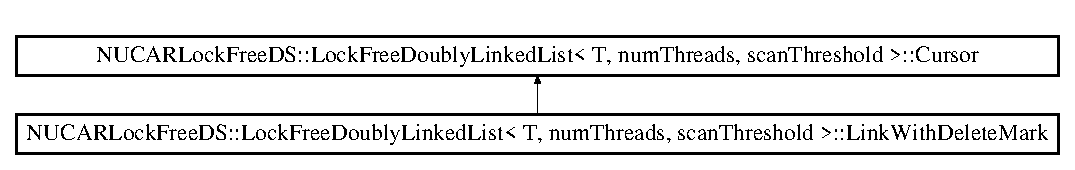
\includegraphics[height=1.839080cm]{class_n_u_c_a_r_lock_free_d_s_1_1_lock_free_doubly_linked_list_1_1_link_with_delete_mark}
\end{center}
\end{figure}
\subsection*{Public Member Functions}
\begin{DoxyCompactItemize}
\item 
\+\_\+\+\_\+device\+\_\+\+\_\+ \mbox{\hyperlink{class_n_u_c_a_r_lock_free_d_s_1_1_lock_free_doubly_linked_list_abb8fd1da564d74028552e980bc99a704}{Node\+\_\+t}} $\ast$ \mbox{\hyperlink{class_n_u_c_a_r_lock_free_d_s_1_1_lock_free_doubly_linked_list_1_1_link_with_delete_mark_a3f9ae9e135b17122984dbf716b46b951}{Get\+Node}} () const
\item 
\+\_\+\+\_\+device\+\_\+\+\_\+ bool \mbox{\hyperlink{class_n_u_c_a_r_lock_free_d_s_1_1_lock_free_doubly_linked_list_1_1_link_with_delete_mark_abd04793481353e77ddce79d713720e78}{d}} () const
\item 
\+\_\+\+\_\+device\+\_\+\+\_\+ \mbox{\hyperlink{class_n_u_c_a_r_lock_free_d_s_1_1_allocator_a3931e84d06ddd3b436103475197eb12a}{Allocator\+\_\+t\+::\+Pointer\+\_\+t}} \mbox{\hyperlink{class_n_u_c_a_r_lock_free_d_s_1_1_lock_free_doubly_linked_list_1_1_link_with_delete_mark_a8f162da8ad41d7cff01e66808b56cbd7}{Get\+Value}} () const
\item 
\+\_\+\+\_\+device\+\_\+\+\_\+ \mbox{\hyperlink{class_n_u_c_a_r_lock_free_d_s_1_1_lock_free_doubly_linked_list_1_1_link_with_delete_mark_a07b869cca6744dad3fef8ea26279b570}{Link\+With\+Delete\+Mark}} (\mbox{\hyperlink{class_n_u_c_a_r_lock_free_d_s_1_1_lock_free_doubly_linked_list_abb8fd1da564d74028552e980bc99a704}{Node\+\_\+t}} $\ast$ilink, const bool delete\+Mark)
\item 
\+\_\+\+\_\+device\+\_\+\+\_\+ \mbox{\hyperlink{class_n_u_c_a_r_lock_free_d_s_1_1_lock_free_doubly_linked_list_1_1_link_with_delete_mark_aedead35ab7fcb097d8bfdaf1178afb1c}{Link\+With\+Delete\+Mark}} (\mbox{\hyperlink{class_n_u_c_a_r_lock_free_d_s_1_1_lock_free_doubly_linked_list_abb8fd1da564d74028552e980bc99a704}{Node\+\_\+t}} $\ast$ilink)
\item 
\+\_\+\+\_\+device\+\_\+\+\_\+ \mbox{\hyperlink{class_n_u_c_a_r_lock_free_d_s_1_1_lock_free_doubly_linked_list_1_1_link_with_delete_mark_ac3ab968f96ba442b40d9bc8bd48a7604}{Link\+With\+Delete\+Mark}} (const \mbox{\hyperlink{class_n_u_c_a_r_lock_free_d_s_1_1_lock_free_doubly_linked_list_1_1_link_with_delete_mark}{Link\+With\+Delete\+Mark}} \&other, const bool delete\+Mark)
\item 
\+\_\+\+\_\+device\+\_\+\+\_\+ \mbox{\hyperlink{class_n_u_c_a_r_lock_free_d_s_1_1_lock_free_doubly_linked_list_1_1_link_with_delete_mark_a7b9929a559282ece56e8ae86c6c0957b}{Link\+With\+Delete\+Mark}} (const \mbox{\hyperlink{class_n_u_c_a_r_lock_free_d_s_1_1_allocator_a3931e84d06ddd3b436103475197eb12a}{Allocator\+\_\+t\+::\+Pointer\+\_\+t}} \&value)
\item 
\+\_\+\+\_\+device\+\_\+\+\_\+ \mbox{\hyperlink{class_n_u_c_a_r_lock_free_d_s_1_1_lock_free_doubly_linked_list_1_1_link_with_delete_mark_a7d7dfc1c8216fb02ed3ccaae5684eed3}{Link\+With\+Delete\+Mark}} ()
\item 
\+\_\+\+\_\+device\+\_\+\+\_\+ bool \mbox{\hyperlink{class_n_u_c_a_r_lock_free_d_s_1_1_lock_free_doubly_linked_list_1_1_link_with_delete_mark_afa41d48d9810b94ed0f2b3d1b6fd52a8}{operator==}} (const \mbox{\hyperlink{class_n_u_c_a_r_lock_free_d_s_1_1_lock_free_doubly_linked_list_1_1_link_with_delete_mark}{Link\+With\+Delete\+Mark}} \&other) const
\item 
\+\_\+\+\_\+device\+\_\+\+\_\+ bool \mbox{\hyperlink{class_n_u_c_a_r_lock_free_d_s_1_1_lock_free_doubly_linked_list_1_1_link_with_delete_mark_a347dba997df64a60d2d9bc2d42948c09}{operator!=}} (const \mbox{\hyperlink{class_n_u_c_a_r_lock_free_d_s_1_1_lock_free_doubly_linked_list_1_1_link_with_delete_mark}{Link\+With\+Delete\+Mark}} \&other) const
\end{DoxyCompactItemize}
\subsection*{Static Public Member Functions}
\begin{DoxyCompactItemize}
\item 
static \+\_\+\+\_\+device\+\_\+\+\_\+ void \mbox{\hyperlink{class_n_u_c_a_r_lock_free_d_s_1_1_lock_free_doubly_linked_list_1_1_link_with_delete_mark_afc16efcd81c1c4593f90f37d6360ff1d}{Set\+Mark}} (\mbox{\hyperlink{class_n_u_c_a_r_lock_free_d_s_1_1_lock_free_doubly_linked_list_1_1_link_with_delete_mark}{Link\+With\+Delete\+Mark}} $\ast$\mbox{\hyperlink{class_n_u_c_a_r_lock_free_d_s_1_1_lock_free_doubly_linked_list_1_1_link_with_delete_mark_aa3e6d661a7dfd3ebeca045ddb2fe07dc}{link}})
\end{DoxyCompactItemize}
\subsection*{Private Attributes}
\begin{DoxyCompactItemize}
\item 
\mbox{\hyperlink{class_n_u_c_a_r_lock_free_d_s_1_1_allocator_a3931e84d06ddd3b436103475197eb12a}{Allocator\+\_\+t\+::\+Pointer\+\_\+t}} \mbox{\hyperlink{class_n_u_c_a_r_lock_free_d_s_1_1_lock_free_doubly_linked_list_1_1_link_with_delete_mark_aa3e6d661a7dfd3ebeca045ddb2fe07dc}{link}}
\end{DoxyCompactItemize}
\subsection*{Static Private Attributes}
\begin{DoxyCompactItemize}
\item 
static constexpr \mbox{\hyperlink{class_n_u_c_a_r_lock_free_d_s_1_1_allocator_a3931e84d06ddd3b436103475197eb12a}{Allocator\+\_\+t\+::\+Pointer\+\_\+t}} \mbox{\hyperlink{class_n_u_c_a_r_lock_free_d_s_1_1_lock_free_doubly_linked_list_1_1_link_with_delete_mark_af670d4e1c35ee581cbc55ec70e1de6c4}{link\+Delete\+Flag\+Mask}} = 1
\item 
static constexpr \mbox{\hyperlink{class_n_u_c_a_r_lock_free_d_s_1_1_allocator_a3931e84d06ddd3b436103475197eb12a}{Allocator\+\_\+t\+::\+Pointer\+\_\+t}} \mbox{\hyperlink{class_n_u_c_a_r_lock_free_d_s_1_1_lock_free_doubly_linked_list_1_1_link_with_delete_mark_a9a0d4322dd840571fa886b966618d9a9}{link\+Pointer\+Mask}} = $\sim$\mbox{\hyperlink{class_n_u_c_a_r_lock_free_d_s_1_1_lock_free_doubly_linked_list_1_1_link_with_delete_mark_af670d4e1c35ee581cbc55ec70e1de6c4}{link\+Delete\+Flag\+Mask}}
\end{DoxyCompactItemize}


\subsection{Constructor \& Destructor Documentation}
\mbox{\Hypertarget{class_n_u_c_a_r_lock_free_d_s_1_1_lock_free_doubly_linked_list_1_1_link_with_delete_mark_a07b869cca6744dad3fef8ea26279b570}\label{class_n_u_c_a_r_lock_free_d_s_1_1_lock_free_doubly_linked_list_1_1_link_with_delete_mark_a07b869cca6744dad3fef8ea26279b570}} 
\index{N\+U\+C\+A\+R\+Lock\+Free\+D\+S\+::\+Lock\+Free\+Doubly\+Linked\+List\+::\+Link\+With\+Delete\+Mark@{N\+U\+C\+A\+R\+Lock\+Free\+D\+S\+::\+Lock\+Free\+Doubly\+Linked\+List\+::\+Link\+With\+Delete\+Mark}!Link\+With\+Delete\+Mark@{Link\+With\+Delete\+Mark}}
\index{Link\+With\+Delete\+Mark@{Link\+With\+Delete\+Mark}!N\+U\+C\+A\+R\+Lock\+Free\+D\+S\+::\+Lock\+Free\+Doubly\+Linked\+List\+::\+Link\+With\+Delete\+Mark@{N\+U\+C\+A\+R\+Lock\+Free\+D\+S\+::\+Lock\+Free\+Doubly\+Linked\+List\+::\+Link\+With\+Delete\+Mark}}
\subsubsection{\texorpdfstring{Link\+With\+Delete\+Mark()}{LinkWithDeleteMark()}\hspace{0.1cm}{\footnotesize\ttfamily [1/5]}}
{\footnotesize\ttfamily template$<$typename T , Lock\+Free\+Doubly\+Linked\+List\+Config\+::\+Doubly\+Linked\+List\+Index\+\_\+t num\+Threads, Lock\+Free\+Doubly\+Linked\+List\+Config\+::\+Doubly\+Linked\+List\+Index\+\_\+t scan\+Threshold = Lock\+Free\+Doubly\+Linked\+List\+Config\+::\+Get\+Default\+Scan\+Threshold$<$\+Lock\+Free\+Doubly\+Linked\+List\+Config\+::\+Doubly\+Linked\+List\+Index\+\_\+t$>$(num\+Threads)$>$ \\
\+\_\+\+\_\+device\+\_\+\+\_\+ \mbox{\hyperlink{class_n_u_c_a_r_lock_free_d_s_1_1_lock_free_doubly_linked_list}{N\+U\+C\+A\+R\+Lock\+Free\+D\+S\+::\+Lock\+Free\+Doubly\+Linked\+List}}$<$ T, num\+Threads, scan\+Threshold $>$\+::Link\+With\+Delete\+Mark\+::\+Link\+With\+Delete\+Mark (\begin{DoxyParamCaption}\item[{\mbox{\hyperlink{class_n_u_c_a_r_lock_free_d_s_1_1_lock_free_doubly_linked_list_abb8fd1da564d74028552e980bc99a704}{Node\+\_\+t}} $\ast$}]{ilink,  }\item[{const bool}]{delete\+Mark }\end{DoxyParamCaption})\hspace{0.3cm}{\ttfamily [inline]}}

\mbox{\Hypertarget{class_n_u_c_a_r_lock_free_d_s_1_1_lock_free_doubly_linked_list_1_1_link_with_delete_mark_aedead35ab7fcb097d8bfdaf1178afb1c}\label{class_n_u_c_a_r_lock_free_d_s_1_1_lock_free_doubly_linked_list_1_1_link_with_delete_mark_aedead35ab7fcb097d8bfdaf1178afb1c}} 
\index{N\+U\+C\+A\+R\+Lock\+Free\+D\+S\+::\+Lock\+Free\+Doubly\+Linked\+List\+::\+Link\+With\+Delete\+Mark@{N\+U\+C\+A\+R\+Lock\+Free\+D\+S\+::\+Lock\+Free\+Doubly\+Linked\+List\+::\+Link\+With\+Delete\+Mark}!Link\+With\+Delete\+Mark@{Link\+With\+Delete\+Mark}}
\index{Link\+With\+Delete\+Mark@{Link\+With\+Delete\+Mark}!N\+U\+C\+A\+R\+Lock\+Free\+D\+S\+::\+Lock\+Free\+Doubly\+Linked\+List\+::\+Link\+With\+Delete\+Mark@{N\+U\+C\+A\+R\+Lock\+Free\+D\+S\+::\+Lock\+Free\+Doubly\+Linked\+List\+::\+Link\+With\+Delete\+Mark}}
\subsubsection{\texorpdfstring{Link\+With\+Delete\+Mark()}{LinkWithDeleteMark()}\hspace{0.1cm}{\footnotesize\ttfamily [2/5]}}
{\footnotesize\ttfamily template$<$typename T , Lock\+Free\+Doubly\+Linked\+List\+Config\+::\+Doubly\+Linked\+List\+Index\+\_\+t num\+Threads, Lock\+Free\+Doubly\+Linked\+List\+Config\+::\+Doubly\+Linked\+List\+Index\+\_\+t scan\+Threshold = Lock\+Free\+Doubly\+Linked\+List\+Config\+::\+Get\+Default\+Scan\+Threshold$<$\+Lock\+Free\+Doubly\+Linked\+List\+Config\+::\+Doubly\+Linked\+List\+Index\+\_\+t$>$(num\+Threads)$>$ \\
\+\_\+\+\_\+device\+\_\+\+\_\+ \mbox{\hyperlink{class_n_u_c_a_r_lock_free_d_s_1_1_lock_free_doubly_linked_list}{N\+U\+C\+A\+R\+Lock\+Free\+D\+S\+::\+Lock\+Free\+Doubly\+Linked\+List}}$<$ T, num\+Threads, scan\+Threshold $>$\+::Link\+With\+Delete\+Mark\+::\+Link\+With\+Delete\+Mark (\begin{DoxyParamCaption}\item[{\mbox{\hyperlink{class_n_u_c_a_r_lock_free_d_s_1_1_lock_free_doubly_linked_list_abb8fd1da564d74028552e980bc99a704}{Node\+\_\+t}} $\ast$}]{ilink }\end{DoxyParamCaption})\hspace{0.3cm}{\ttfamily [inline]}}

\mbox{\Hypertarget{class_n_u_c_a_r_lock_free_d_s_1_1_lock_free_doubly_linked_list_1_1_link_with_delete_mark_ac3ab968f96ba442b40d9bc8bd48a7604}\label{class_n_u_c_a_r_lock_free_d_s_1_1_lock_free_doubly_linked_list_1_1_link_with_delete_mark_ac3ab968f96ba442b40d9bc8bd48a7604}} 
\index{N\+U\+C\+A\+R\+Lock\+Free\+D\+S\+::\+Lock\+Free\+Doubly\+Linked\+List\+::\+Link\+With\+Delete\+Mark@{N\+U\+C\+A\+R\+Lock\+Free\+D\+S\+::\+Lock\+Free\+Doubly\+Linked\+List\+::\+Link\+With\+Delete\+Mark}!Link\+With\+Delete\+Mark@{Link\+With\+Delete\+Mark}}
\index{Link\+With\+Delete\+Mark@{Link\+With\+Delete\+Mark}!N\+U\+C\+A\+R\+Lock\+Free\+D\+S\+::\+Lock\+Free\+Doubly\+Linked\+List\+::\+Link\+With\+Delete\+Mark@{N\+U\+C\+A\+R\+Lock\+Free\+D\+S\+::\+Lock\+Free\+Doubly\+Linked\+List\+::\+Link\+With\+Delete\+Mark}}
\subsubsection{\texorpdfstring{Link\+With\+Delete\+Mark()}{LinkWithDeleteMark()}\hspace{0.1cm}{\footnotesize\ttfamily [3/5]}}
{\footnotesize\ttfamily template$<$typename T , Lock\+Free\+Doubly\+Linked\+List\+Config\+::\+Doubly\+Linked\+List\+Index\+\_\+t num\+Threads, Lock\+Free\+Doubly\+Linked\+List\+Config\+::\+Doubly\+Linked\+List\+Index\+\_\+t scan\+Threshold = Lock\+Free\+Doubly\+Linked\+List\+Config\+::\+Get\+Default\+Scan\+Threshold$<$\+Lock\+Free\+Doubly\+Linked\+List\+Config\+::\+Doubly\+Linked\+List\+Index\+\_\+t$>$(num\+Threads)$>$ \\
\+\_\+\+\_\+device\+\_\+\+\_\+ \mbox{\hyperlink{class_n_u_c_a_r_lock_free_d_s_1_1_lock_free_doubly_linked_list}{N\+U\+C\+A\+R\+Lock\+Free\+D\+S\+::\+Lock\+Free\+Doubly\+Linked\+List}}$<$ T, num\+Threads, scan\+Threshold $>$\+::Link\+With\+Delete\+Mark\+::\+Link\+With\+Delete\+Mark (\begin{DoxyParamCaption}\item[{const \mbox{\hyperlink{class_n_u_c_a_r_lock_free_d_s_1_1_lock_free_doubly_linked_list_1_1_link_with_delete_mark}{Link\+With\+Delete\+Mark}} \&}]{other,  }\item[{const bool}]{delete\+Mark }\end{DoxyParamCaption})\hspace{0.3cm}{\ttfamily [inline]}}

\mbox{\Hypertarget{class_n_u_c_a_r_lock_free_d_s_1_1_lock_free_doubly_linked_list_1_1_link_with_delete_mark_a7b9929a559282ece56e8ae86c6c0957b}\label{class_n_u_c_a_r_lock_free_d_s_1_1_lock_free_doubly_linked_list_1_1_link_with_delete_mark_a7b9929a559282ece56e8ae86c6c0957b}} 
\index{N\+U\+C\+A\+R\+Lock\+Free\+D\+S\+::\+Lock\+Free\+Doubly\+Linked\+List\+::\+Link\+With\+Delete\+Mark@{N\+U\+C\+A\+R\+Lock\+Free\+D\+S\+::\+Lock\+Free\+Doubly\+Linked\+List\+::\+Link\+With\+Delete\+Mark}!Link\+With\+Delete\+Mark@{Link\+With\+Delete\+Mark}}
\index{Link\+With\+Delete\+Mark@{Link\+With\+Delete\+Mark}!N\+U\+C\+A\+R\+Lock\+Free\+D\+S\+::\+Lock\+Free\+Doubly\+Linked\+List\+::\+Link\+With\+Delete\+Mark@{N\+U\+C\+A\+R\+Lock\+Free\+D\+S\+::\+Lock\+Free\+Doubly\+Linked\+List\+::\+Link\+With\+Delete\+Mark}}
\subsubsection{\texorpdfstring{Link\+With\+Delete\+Mark()}{LinkWithDeleteMark()}\hspace{0.1cm}{\footnotesize\ttfamily [4/5]}}
{\footnotesize\ttfamily template$<$typename T , Lock\+Free\+Doubly\+Linked\+List\+Config\+::\+Doubly\+Linked\+List\+Index\+\_\+t num\+Threads, Lock\+Free\+Doubly\+Linked\+List\+Config\+::\+Doubly\+Linked\+List\+Index\+\_\+t scan\+Threshold = Lock\+Free\+Doubly\+Linked\+List\+Config\+::\+Get\+Default\+Scan\+Threshold$<$\+Lock\+Free\+Doubly\+Linked\+List\+Config\+::\+Doubly\+Linked\+List\+Index\+\_\+t$>$(num\+Threads)$>$ \\
\+\_\+\+\_\+device\+\_\+\+\_\+ \mbox{\hyperlink{class_n_u_c_a_r_lock_free_d_s_1_1_lock_free_doubly_linked_list}{N\+U\+C\+A\+R\+Lock\+Free\+D\+S\+::\+Lock\+Free\+Doubly\+Linked\+List}}$<$ T, num\+Threads, scan\+Threshold $>$\+::Link\+With\+Delete\+Mark\+::\+Link\+With\+Delete\+Mark (\begin{DoxyParamCaption}\item[{const \mbox{\hyperlink{class_n_u_c_a_r_lock_free_d_s_1_1_allocator_a3931e84d06ddd3b436103475197eb12a}{Allocator\+\_\+t\+::\+Pointer\+\_\+t}} \&}]{value }\end{DoxyParamCaption})\hspace{0.3cm}{\ttfamily [inline]}}

\mbox{\Hypertarget{class_n_u_c_a_r_lock_free_d_s_1_1_lock_free_doubly_linked_list_1_1_link_with_delete_mark_a7d7dfc1c8216fb02ed3ccaae5684eed3}\label{class_n_u_c_a_r_lock_free_d_s_1_1_lock_free_doubly_linked_list_1_1_link_with_delete_mark_a7d7dfc1c8216fb02ed3ccaae5684eed3}} 
\index{N\+U\+C\+A\+R\+Lock\+Free\+D\+S\+::\+Lock\+Free\+Doubly\+Linked\+List\+::\+Link\+With\+Delete\+Mark@{N\+U\+C\+A\+R\+Lock\+Free\+D\+S\+::\+Lock\+Free\+Doubly\+Linked\+List\+::\+Link\+With\+Delete\+Mark}!Link\+With\+Delete\+Mark@{Link\+With\+Delete\+Mark}}
\index{Link\+With\+Delete\+Mark@{Link\+With\+Delete\+Mark}!N\+U\+C\+A\+R\+Lock\+Free\+D\+S\+::\+Lock\+Free\+Doubly\+Linked\+List\+::\+Link\+With\+Delete\+Mark@{N\+U\+C\+A\+R\+Lock\+Free\+D\+S\+::\+Lock\+Free\+Doubly\+Linked\+List\+::\+Link\+With\+Delete\+Mark}}
\subsubsection{\texorpdfstring{Link\+With\+Delete\+Mark()}{LinkWithDeleteMark()}\hspace{0.1cm}{\footnotesize\ttfamily [5/5]}}
{\footnotesize\ttfamily template$<$typename T , Lock\+Free\+Doubly\+Linked\+List\+Config\+::\+Doubly\+Linked\+List\+Index\+\_\+t num\+Threads, Lock\+Free\+Doubly\+Linked\+List\+Config\+::\+Doubly\+Linked\+List\+Index\+\_\+t scan\+Threshold = Lock\+Free\+Doubly\+Linked\+List\+Config\+::\+Get\+Default\+Scan\+Threshold$<$\+Lock\+Free\+Doubly\+Linked\+List\+Config\+::\+Doubly\+Linked\+List\+Index\+\_\+t$>$(num\+Threads)$>$ \\
\+\_\+\+\_\+device\+\_\+\+\_\+ \mbox{\hyperlink{class_n_u_c_a_r_lock_free_d_s_1_1_lock_free_doubly_linked_list}{N\+U\+C\+A\+R\+Lock\+Free\+D\+S\+::\+Lock\+Free\+Doubly\+Linked\+List}}$<$ T, num\+Threads, scan\+Threshold $>$\+::Link\+With\+Delete\+Mark\+::\+Link\+With\+Delete\+Mark (\begin{DoxyParamCaption}{ }\end{DoxyParamCaption})\hspace{0.3cm}{\ttfamily [inline]}}



\subsection{Member Function Documentation}
\mbox{\Hypertarget{class_n_u_c_a_r_lock_free_d_s_1_1_lock_free_doubly_linked_list_1_1_link_with_delete_mark_abd04793481353e77ddce79d713720e78}\label{class_n_u_c_a_r_lock_free_d_s_1_1_lock_free_doubly_linked_list_1_1_link_with_delete_mark_abd04793481353e77ddce79d713720e78}} 
\index{N\+U\+C\+A\+R\+Lock\+Free\+D\+S\+::\+Lock\+Free\+Doubly\+Linked\+List\+::\+Link\+With\+Delete\+Mark@{N\+U\+C\+A\+R\+Lock\+Free\+D\+S\+::\+Lock\+Free\+Doubly\+Linked\+List\+::\+Link\+With\+Delete\+Mark}!d@{d}}
\index{d@{d}!N\+U\+C\+A\+R\+Lock\+Free\+D\+S\+::\+Lock\+Free\+Doubly\+Linked\+List\+::\+Link\+With\+Delete\+Mark@{N\+U\+C\+A\+R\+Lock\+Free\+D\+S\+::\+Lock\+Free\+Doubly\+Linked\+List\+::\+Link\+With\+Delete\+Mark}}
\subsubsection{\texorpdfstring{d()}{d()}}
{\footnotesize\ttfamily template$<$typename T , Lock\+Free\+Doubly\+Linked\+List\+Config\+::\+Doubly\+Linked\+List\+Index\+\_\+t num\+Threads, Lock\+Free\+Doubly\+Linked\+List\+Config\+::\+Doubly\+Linked\+List\+Index\+\_\+t scan\+Threshold = Lock\+Free\+Doubly\+Linked\+List\+Config\+::\+Get\+Default\+Scan\+Threshold$<$\+Lock\+Free\+Doubly\+Linked\+List\+Config\+::\+Doubly\+Linked\+List\+Index\+\_\+t$>$(num\+Threads)$>$ \\
\+\_\+\+\_\+device\+\_\+\+\_\+ bool \mbox{\hyperlink{class_n_u_c_a_r_lock_free_d_s_1_1_lock_free_doubly_linked_list}{N\+U\+C\+A\+R\+Lock\+Free\+D\+S\+::\+Lock\+Free\+Doubly\+Linked\+List}}$<$ T, num\+Threads, scan\+Threshold $>$\+::Link\+With\+Delete\+Mark\+::d (\begin{DoxyParamCaption}{ }\end{DoxyParamCaption}) const\hspace{0.3cm}{\ttfamily [inline]}}

\mbox{\Hypertarget{class_n_u_c_a_r_lock_free_d_s_1_1_lock_free_doubly_linked_list_1_1_link_with_delete_mark_a3f9ae9e135b17122984dbf716b46b951}\label{class_n_u_c_a_r_lock_free_d_s_1_1_lock_free_doubly_linked_list_1_1_link_with_delete_mark_a3f9ae9e135b17122984dbf716b46b951}} 
\index{N\+U\+C\+A\+R\+Lock\+Free\+D\+S\+::\+Lock\+Free\+Doubly\+Linked\+List\+::\+Link\+With\+Delete\+Mark@{N\+U\+C\+A\+R\+Lock\+Free\+D\+S\+::\+Lock\+Free\+Doubly\+Linked\+List\+::\+Link\+With\+Delete\+Mark}!Get\+Node@{Get\+Node}}
\index{Get\+Node@{Get\+Node}!N\+U\+C\+A\+R\+Lock\+Free\+D\+S\+::\+Lock\+Free\+Doubly\+Linked\+List\+::\+Link\+With\+Delete\+Mark@{N\+U\+C\+A\+R\+Lock\+Free\+D\+S\+::\+Lock\+Free\+Doubly\+Linked\+List\+::\+Link\+With\+Delete\+Mark}}
\subsubsection{\texorpdfstring{Get\+Node()}{GetNode()}}
{\footnotesize\ttfamily template$<$typename T , Lock\+Free\+Doubly\+Linked\+List\+Config\+::\+Doubly\+Linked\+List\+Index\+\_\+t num\+Threads, Lock\+Free\+Doubly\+Linked\+List\+Config\+::\+Doubly\+Linked\+List\+Index\+\_\+t scan\+Threshold = Lock\+Free\+Doubly\+Linked\+List\+Config\+::\+Get\+Default\+Scan\+Threshold$<$\+Lock\+Free\+Doubly\+Linked\+List\+Config\+::\+Doubly\+Linked\+List\+Index\+\_\+t$>$(num\+Threads)$>$ \\
\+\_\+\+\_\+device\+\_\+\+\_\+ \mbox{\hyperlink{class_n_u_c_a_r_lock_free_d_s_1_1_lock_free_doubly_linked_list_abb8fd1da564d74028552e980bc99a704}{Node\+\_\+t}}$\ast$ \mbox{\hyperlink{class_n_u_c_a_r_lock_free_d_s_1_1_lock_free_doubly_linked_list}{N\+U\+C\+A\+R\+Lock\+Free\+D\+S\+::\+Lock\+Free\+Doubly\+Linked\+List}}$<$ T, num\+Threads, scan\+Threshold $>$\+::Link\+With\+Delete\+Mark\+::\+Get\+Node (\begin{DoxyParamCaption}{ }\end{DoxyParamCaption}) const\hspace{0.3cm}{\ttfamily [inline]}}

\mbox{\Hypertarget{class_n_u_c_a_r_lock_free_d_s_1_1_lock_free_doubly_linked_list_1_1_link_with_delete_mark_a8f162da8ad41d7cff01e66808b56cbd7}\label{class_n_u_c_a_r_lock_free_d_s_1_1_lock_free_doubly_linked_list_1_1_link_with_delete_mark_a8f162da8ad41d7cff01e66808b56cbd7}} 
\index{N\+U\+C\+A\+R\+Lock\+Free\+D\+S\+::\+Lock\+Free\+Doubly\+Linked\+List\+::\+Link\+With\+Delete\+Mark@{N\+U\+C\+A\+R\+Lock\+Free\+D\+S\+::\+Lock\+Free\+Doubly\+Linked\+List\+::\+Link\+With\+Delete\+Mark}!Get\+Value@{Get\+Value}}
\index{Get\+Value@{Get\+Value}!N\+U\+C\+A\+R\+Lock\+Free\+D\+S\+::\+Lock\+Free\+Doubly\+Linked\+List\+::\+Link\+With\+Delete\+Mark@{N\+U\+C\+A\+R\+Lock\+Free\+D\+S\+::\+Lock\+Free\+Doubly\+Linked\+List\+::\+Link\+With\+Delete\+Mark}}
\subsubsection{\texorpdfstring{Get\+Value()}{GetValue()}}
{\footnotesize\ttfamily template$<$typename T , Lock\+Free\+Doubly\+Linked\+List\+Config\+::\+Doubly\+Linked\+List\+Index\+\_\+t num\+Threads, Lock\+Free\+Doubly\+Linked\+List\+Config\+::\+Doubly\+Linked\+List\+Index\+\_\+t scan\+Threshold = Lock\+Free\+Doubly\+Linked\+List\+Config\+::\+Get\+Default\+Scan\+Threshold$<$\+Lock\+Free\+Doubly\+Linked\+List\+Config\+::\+Doubly\+Linked\+List\+Index\+\_\+t$>$(num\+Threads)$>$ \\
\+\_\+\+\_\+device\+\_\+\+\_\+ \mbox{\hyperlink{class_n_u_c_a_r_lock_free_d_s_1_1_allocator_a3931e84d06ddd3b436103475197eb12a}{Allocator\+\_\+t\+::\+Pointer\+\_\+t}} \mbox{\hyperlink{class_n_u_c_a_r_lock_free_d_s_1_1_lock_free_doubly_linked_list}{N\+U\+C\+A\+R\+Lock\+Free\+D\+S\+::\+Lock\+Free\+Doubly\+Linked\+List}}$<$ T, num\+Threads, scan\+Threshold $>$\+::Link\+With\+Delete\+Mark\+::\+Get\+Value (\begin{DoxyParamCaption}{ }\end{DoxyParamCaption}) const\hspace{0.3cm}{\ttfamily [inline]}}

\mbox{\Hypertarget{class_n_u_c_a_r_lock_free_d_s_1_1_lock_free_doubly_linked_list_1_1_link_with_delete_mark_a347dba997df64a60d2d9bc2d42948c09}\label{class_n_u_c_a_r_lock_free_d_s_1_1_lock_free_doubly_linked_list_1_1_link_with_delete_mark_a347dba997df64a60d2d9bc2d42948c09}} 
\index{N\+U\+C\+A\+R\+Lock\+Free\+D\+S\+::\+Lock\+Free\+Doubly\+Linked\+List\+::\+Link\+With\+Delete\+Mark@{N\+U\+C\+A\+R\+Lock\+Free\+D\+S\+::\+Lock\+Free\+Doubly\+Linked\+List\+::\+Link\+With\+Delete\+Mark}!operator"!=@{operator"!=}}
\index{operator"!=@{operator"!=}!N\+U\+C\+A\+R\+Lock\+Free\+D\+S\+::\+Lock\+Free\+Doubly\+Linked\+List\+::\+Link\+With\+Delete\+Mark@{N\+U\+C\+A\+R\+Lock\+Free\+D\+S\+::\+Lock\+Free\+Doubly\+Linked\+List\+::\+Link\+With\+Delete\+Mark}}
\subsubsection{\texorpdfstring{operator"!=()}{operator!=()}}
{\footnotesize\ttfamily template$<$typename T , Lock\+Free\+Doubly\+Linked\+List\+Config\+::\+Doubly\+Linked\+List\+Index\+\_\+t num\+Threads, Lock\+Free\+Doubly\+Linked\+List\+Config\+::\+Doubly\+Linked\+List\+Index\+\_\+t scan\+Threshold = Lock\+Free\+Doubly\+Linked\+List\+Config\+::\+Get\+Default\+Scan\+Threshold$<$\+Lock\+Free\+Doubly\+Linked\+List\+Config\+::\+Doubly\+Linked\+List\+Index\+\_\+t$>$(num\+Threads)$>$ \\
\+\_\+\+\_\+device\+\_\+\+\_\+ bool \mbox{\hyperlink{class_n_u_c_a_r_lock_free_d_s_1_1_lock_free_doubly_linked_list}{N\+U\+C\+A\+R\+Lock\+Free\+D\+S\+::\+Lock\+Free\+Doubly\+Linked\+List}}$<$ T, num\+Threads, scan\+Threshold $>$\+::Link\+With\+Delete\+Mark\+::operator!= (\begin{DoxyParamCaption}\item[{const \mbox{\hyperlink{class_n_u_c_a_r_lock_free_d_s_1_1_lock_free_doubly_linked_list_1_1_link_with_delete_mark}{Link\+With\+Delete\+Mark}} \&}]{other }\end{DoxyParamCaption}) const\hspace{0.3cm}{\ttfamily [inline]}}

\mbox{\Hypertarget{class_n_u_c_a_r_lock_free_d_s_1_1_lock_free_doubly_linked_list_1_1_link_with_delete_mark_afa41d48d9810b94ed0f2b3d1b6fd52a8}\label{class_n_u_c_a_r_lock_free_d_s_1_1_lock_free_doubly_linked_list_1_1_link_with_delete_mark_afa41d48d9810b94ed0f2b3d1b6fd52a8}} 
\index{N\+U\+C\+A\+R\+Lock\+Free\+D\+S\+::\+Lock\+Free\+Doubly\+Linked\+List\+::\+Link\+With\+Delete\+Mark@{N\+U\+C\+A\+R\+Lock\+Free\+D\+S\+::\+Lock\+Free\+Doubly\+Linked\+List\+::\+Link\+With\+Delete\+Mark}!operator==@{operator==}}
\index{operator==@{operator==}!N\+U\+C\+A\+R\+Lock\+Free\+D\+S\+::\+Lock\+Free\+Doubly\+Linked\+List\+::\+Link\+With\+Delete\+Mark@{N\+U\+C\+A\+R\+Lock\+Free\+D\+S\+::\+Lock\+Free\+Doubly\+Linked\+List\+::\+Link\+With\+Delete\+Mark}}
\subsubsection{\texorpdfstring{operator==()}{operator==()}}
{\footnotesize\ttfamily template$<$typename T , Lock\+Free\+Doubly\+Linked\+List\+Config\+::\+Doubly\+Linked\+List\+Index\+\_\+t num\+Threads, Lock\+Free\+Doubly\+Linked\+List\+Config\+::\+Doubly\+Linked\+List\+Index\+\_\+t scan\+Threshold = Lock\+Free\+Doubly\+Linked\+List\+Config\+::\+Get\+Default\+Scan\+Threshold$<$\+Lock\+Free\+Doubly\+Linked\+List\+Config\+::\+Doubly\+Linked\+List\+Index\+\_\+t$>$(num\+Threads)$>$ \\
\+\_\+\+\_\+device\+\_\+\+\_\+ bool \mbox{\hyperlink{class_n_u_c_a_r_lock_free_d_s_1_1_lock_free_doubly_linked_list}{N\+U\+C\+A\+R\+Lock\+Free\+D\+S\+::\+Lock\+Free\+Doubly\+Linked\+List}}$<$ T, num\+Threads, scan\+Threshold $>$\+::Link\+With\+Delete\+Mark\+::operator== (\begin{DoxyParamCaption}\item[{const \mbox{\hyperlink{class_n_u_c_a_r_lock_free_d_s_1_1_lock_free_doubly_linked_list_1_1_link_with_delete_mark}{Link\+With\+Delete\+Mark}} \&}]{other }\end{DoxyParamCaption}) const\hspace{0.3cm}{\ttfamily [inline]}}

\mbox{\Hypertarget{class_n_u_c_a_r_lock_free_d_s_1_1_lock_free_doubly_linked_list_1_1_link_with_delete_mark_afc16efcd81c1c4593f90f37d6360ff1d}\label{class_n_u_c_a_r_lock_free_d_s_1_1_lock_free_doubly_linked_list_1_1_link_with_delete_mark_afc16efcd81c1c4593f90f37d6360ff1d}} 
\index{N\+U\+C\+A\+R\+Lock\+Free\+D\+S\+::\+Lock\+Free\+Doubly\+Linked\+List\+::\+Link\+With\+Delete\+Mark@{N\+U\+C\+A\+R\+Lock\+Free\+D\+S\+::\+Lock\+Free\+Doubly\+Linked\+List\+::\+Link\+With\+Delete\+Mark}!Set\+Mark@{Set\+Mark}}
\index{Set\+Mark@{Set\+Mark}!N\+U\+C\+A\+R\+Lock\+Free\+D\+S\+::\+Lock\+Free\+Doubly\+Linked\+List\+::\+Link\+With\+Delete\+Mark@{N\+U\+C\+A\+R\+Lock\+Free\+D\+S\+::\+Lock\+Free\+Doubly\+Linked\+List\+::\+Link\+With\+Delete\+Mark}}
\subsubsection{\texorpdfstring{Set\+Mark()}{SetMark()}}
{\footnotesize\ttfamily template$<$typename T , Lock\+Free\+Doubly\+Linked\+List\+Config\+::\+Doubly\+Linked\+List\+Index\+\_\+t num\+Threads, Lock\+Free\+Doubly\+Linked\+List\+Config\+::\+Doubly\+Linked\+List\+Index\+\_\+t scan\+Threshold = Lock\+Free\+Doubly\+Linked\+List\+Config\+::\+Get\+Default\+Scan\+Threshold$<$\+Lock\+Free\+Doubly\+Linked\+List\+Config\+::\+Doubly\+Linked\+List\+Index\+\_\+t$>$(num\+Threads)$>$ \\
static \+\_\+\+\_\+device\+\_\+\+\_\+ void \mbox{\hyperlink{class_n_u_c_a_r_lock_free_d_s_1_1_lock_free_doubly_linked_list}{N\+U\+C\+A\+R\+Lock\+Free\+D\+S\+::\+Lock\+Free\+Doubly\+Linked\+List}}$<$ T, num\+Threads, scan\+Threshold $>$\+::Link\+With\+Delete\+Mark\+::\+Set\+Mark (\begin{DoxyParamCaption}\item[{\mbox{\hyperlink{class_n_u_c_a_r_lock_free_d_s_1_1_lock_free_doubly_linked_list_1_1_link_with_delete_mark}{Link\+With\+Delete\+Mark}} $\ast$}]{link }\end{DoxyParamCaption})\hspace{0.3cm}{\ttfamily [inline]}, {\ttfamily [static]}}



\subsection{Member Data Documentation}
\mbox{\Hypertarget{class_n_u_c_a_r_lock_free_d_s_1_1_lock_free_doubly_linked_list_1_1_link_with_delete_mark_aa3e6d661a7dfd3ebeca045ddb2fe07dc}\label{class_n_u_c_a_r_lock_free_d_s_1_1_lock_free_doubly_linked_list_1_1_link_with_delete_mark_aa3e6d661a7dfd3ebeca045ddb2fe07dc}} 
\index{N\+U\+C\+A\+R\+Lock\+Free\+D\+S\+::\+Lock\+Free\+Doubly\+Linked\+List\+::\+Link\+With\+Delete\+Mark@{N\+U\+C\+A\+R\+Lock\+Free\+D\+S\+::\+Lock\+Free\+Doubly\+Linked\+List\+::\+Link\+With\+Delete\+Mark}!link@{link}}
\index{link@{link}!N\+U\+C\+A\+R\+Lock\+Free\+D\+S\+::\+Lock\+Free\+Doubly\+Linked\+List\+::\+Link\+With\+Delete\+Mark@{N\+U\+C\+A\+R\+Lock\+Free\+D\+S\+::\+Lock\+Free\+Doubly\+Linked\+List\+::\+Link\+With\+Delete\+Mark}}
\subsubsection{\texorpdfstring{link}{link}}
{\footnotesize\ttfamily template$<$typename T , Lock\+Free\+Doubly\+Linked\+List\+Config\+::\+Doubly\+Linked\+List\+Index\+\_\+t num\+Threads, Lock\+Free\+Doubly\+Linked\+List\+Config\+::\+Doubly\+Linked\+List\+Index\+\_\+t scan\+Threshold = Lock\+Free\+Doubly\+Linked\+List\+Config\+::\+Get\+Default\+Scan\+Threshold$<$\+Lock\+Free\+Doubly\+Linked\+List\+Config\+::\+Doubly\+Linked\+List\+Index\+\_\+t$>$(num\+Threads)$>$ \\
\mbox{\hyperlink{class_n_u_c_a_r_lock_free_d_s_1_1_allocator_a3931e84d06ddd3b436103475197eb12a}{Allocator\+\_\+t\+::\+Pointer\+\_\+t}} \mbox{\hyperlink{class_n_u_c_a_r_lock_free_d_s_1_1_lock_free_doubly_linked_list}{N\+U\+C\+A\+R\+Lock\+Free\+D\+S\+::\+Lock\+Free\+Doubly\+Linked\+List}}$<$ T, num\+Threads, scan\+Threshold $>$\+::Link\+With\+Delete\+Mark\+::link\hspace{0.3cm}{\ttfamily [private]}}

\mbox{\Hypertarget{class_n_u_c_a_r_lock_free_d_s_1_1_lock_free_doubly_linked_list_1_1_link_with_delete_mark_af670d4e1c35ee581cbc55ec70e1de6c4}\label{class_n_u_c_a_r_lock_free_d_s_1_1_lock_free_doubly_linked_list_1_1_link_with_delete_mark_af670d4e1c35ee581cbc55ec70e1de6c4}} 
\index{N\+U\+C\+A\+R\+Lock\+Free\+D\+S\+::\+Lock\+Free\+Doubly\+Linked\+List\+::\+Link\+With\+Delete\+Mark@{N\+U\+C\+A\+R\+Lock\+Free\+D\+S\+::\+Lock\+Free\+Doubly\+Linked\+List\+::\+Link\+With\+Delete\+Mark}!link\+Delete\+Flag\+Mask@{link\+Delete\+Flag\+Mask}}
\index{link\+Delete\+Flag\+Mask@{link\+Delete\+Flag\+Mask}!N\+U\+C\+A\+R\+Lock\+Free\+D\+S\+::\+Lock\+Free\+Doubly\+Linked\+List\+::\+Link\+With\+Delete\+Mark@{N\+U\+C\+A\+R\+Lock\+Free\+D\+S\+::\+Lock\+Free\+Doubly\+Linked\+List\+::\+Link\+With\+Delete\+Mark}}
\subsubsection{\texorpdfstring{link\+Delete\+Flag\+Mask}{linkDeleteFlagMask}}
{\footnotesize\ttfamily template$<$typename T , Lock\+Free\+Doubly\+Linked\+List\+Config\+::\+Doubly\+Linked\+List\+Index\+\_\+t num\+Threads, Lock\+Free\+Doubly\+Linked\+List\+Config\+::\+Doubly\+Linked\+List\+Index\+\_\+t scan\+Threshold = Lock\+Free\+Doubly\+Linked\+List\+Config\+::\+Get\+Default\+Scan\+Threshold$<$\+Lock\+Free\+Doubly\+Linked\+List\+Config\+::\+Doubly\+Linked\+List\+Index\+\_\+t$>$(num\+Threads)$>$ \\
constexpr \mbox{\hyperlink{class_n_u_c_a_r_lock_free_d_s_1_1_allocator_a3931e84d06ddd3b436103475197eb12a}{Allocator\+\_\+t\+::\+Pointer\+\_\+t}} \mbox{\hyperlink{class_n_u_c_a_r_lock_free_d_s_1_1_lock_free_doubly_linked_list}{N\+U\+C\+A\+R\+Lock\+Free\+D\+S\+::\+Lock\+Free\+Doubly\+Linked\+List}}$<$ T, num\+Threads, scan\+Threshold $>$\+::Link\+With\+Delete\+Mark\+::link\+Delete\+Flag\+Mask = 1\hspace{0.3cm}{\ttfamily [static]}, {\ttfamily [private]}}

\mbox{\Hypertarget{class_n_u_c_a_r_lock_free_d_s_1_1_lock_free_doubly_linked_list_1_1_link_with_delete_mark_a9a0d4322dd840571fa886b966618d9a9}\label{class_n_u_c_a_r_lock_free_d_s_1_1_lock_free_doubly_linked_list_1_1_link_with_delete_mark_a9a0d4322dd840571fa886b966618d9a9}} 
\index{N\+U\+C\+A\+R\+Lock\+Free\+D\+S\+::\+Lock\+Free\+Doubly\+Linked\+List\+::\+Link\+With\+Delete\+Mark@{N\+U\+C\+A\+R\+Lock\+Free\+D\+S\+::\+Lock\+Free\+Doubly\+Linked\+List\+::\+Link\+With\+Delete\+Mark}!link\+Pointer\+Mask@{link\+Pointer\+Mask}}
\index{link\+Pointer\+Mask@{link\+Pointer\+Mask}!N\+U\+C\+A\+R\+Lock\+Free\+D\+S\+::\+Lock\+Free\+Doubly\+Linked\+List\+::\+Link\+With\+Delete\+Mark@{N\+U\+C\+A\+R\+Lock\+Free\+D\+S\+::\+Lock\+Free\+Doubly\+Linked\+List\+::\+Link\+With\+Delete\+Mark}}
\subsubsection{\texorpdfstring{link\+Pointer\+Mask}{linkPointerMask}}
{\footnotesize\ttfamily template$<$typename T , Lock\+Free\+Doubly\+Linked\+List\+Config\+::\+Doubly\+Linked\+List\+Index\+\_\+t num\+Threads, Lock\+Free\+Doubly\+Linked\+List\+Config\+::\+Doubly\+Linked\+List\+Index\+\_\+t scan\+Threshold = Lock\+Free\+Doubly\+Linked\+List\+Config\+::\+Get\+Default\+Scan\+Threshold$<$\+Lock\+Free\+Doubly\+Linked\+List\+Config\+::\+Doubly\+Linked\+List\+Index\+\_\+t$>$(num\+Threads)$>$ \\
constexpr \mbox{\hyperlink{class_n_u_c_a_r_lock_free_d_s_1_1_allocator_a3931e84d06ddd3b436103475197eb12a}{Allocator\+\_\+t\+::\+Pointer\+\_\+t}} \mbox{\hyperlink{class_n_u_c_a_r_lock_free_d_s_1_1_lock_free_doubly_linked_list}{N\+U\+C\+A\+R\+Lock\+Free\+D\+S\+::\+Lock\+Free\+Doubly\+Linked\+List}}$<$ T, num\+Threads, scan\+Threshold $>$\+::Link\+With\+Delete\+Mark\+::link\+Pointer\+Mask = $\sim$\mbox{\hyperlink{class_n_u_c_a_r_lock_free_d_s_1_1_lock_free_doubly_linked_list_1_1_link_with_delete_mark_af670d4e1c35ee581cbc55ec70e1de6c4}{link\+Delete\+Flag\+Mask}}\hspace{0.3cm}{\ttfamily [static]}, {\ttfamily [private]}}



The documentation for this class was generated from the following file\+:\begin{DoxyCompactItemize}
\item 
G\+P\+U\+Lock\+Free\+Data\+Structures/\mbox{\hyperlink{_lock_free_doubly_linked_list_8hpp}{Lock\+Free\+Doubly\+Linked\+List.\+hpp}}\end{DoxyCompactItemize}

\hypertarget{class_n_u_c_a_r_lock_free_d_s_1_1_lock_free_doubly_linked_list}{}\section{N\+U\+C\+A\+R\+Lock\+Free\+DS\+:\+:Lock\+Free\+Doubly\+Linked\+List$<$ T, num\+Threads, scan\+Threshold $>$ Class Template Reference}
\label{class_n_u_c_a_r_lock_free_d_s_1_1_lock_free_doubly_linked_list}\index{N\+U\+C\+A\+R\+Lock\+Free\+D\+S\+::\+Lock\+Free\+Doubly\+Linked\+List$<$ T, num\+Threads, scan\+Threshold $>$@{N\+U\+C\+A\+R\+Lock\+Free\+D\+S\+::\+Lock\+Free\+Doubly\+Linked\+List$<$ T, num\+Threads, scan\+Threshold $>$}}


{\ttfamily \#include $<$Lock\+Free\+Doubly\+Linked\+List.\+hpp$>$}

\subsection*{Classes}
\begin{DoxyCompactItemize}
\item 
class \mbox{\hyperlink{class_n_u_c_a_r_lock_free_d_s_1_1_lock_free_doubly_linked_list_1_1_clean_up_node_functor}{Clean\+Up\+Node\+Functor}}
\item 
class \mbox{\hyperlink{class_n_u_c_a_r_lock_free_d_s_1_1_lock_free_doubly_linked_list_1_1_cursor}{Cursor}}
\item 
class \mbox{\hyperlink{class_n_u_c_a_r_lock_free_d_s_1_1_lock_free_doubly_linked_list_1_1_linked_list_node}{Linked\+List\+Node}}
\item 
class \mbox{\hyperlink{class_n_u_c_a_r_lock_free_d_s_1_1_lock_free_doubly_linked_list_1_1_link_with_delete_mark}{Link\+With\+Delete\+Mark}}
\item 
class \mbox{\hyperlink{class_n_u_c_a_r_lock_free_d_s_1_1_lock_free_doubly_linked_list_1_1_terminate_node_functor}{Terminate\+Node\+Functor}}
\item 
class \mbox{\hyperlink{class_n_u_c_a_r_lock_free_d_s_1_1_lock_free_doubly_linked_list_1_1_this_thread_functor}{This\+Thread\+Functor}}
\end{DoxyCompactItemize}
\subsection*{Public Member Functions}
\begin{DoxyCompactItemize}
\item 
\+\_\+\+\_\+device\+\_\+\+\_\+ \mbox{\hyperlink{class_n_u_c_a_r_lock_free_d_s_1_1_lock_free_doubly_linked_list_a79b2e6c603e8c7f8f6bb0ca6b9be21f0}{Lock\+Free\+Doubly\+Linked\+List}} ()
\item 
\+\_\+\+\_\+device\+\_\+\+\_\+ \mbox{\hyperlink{class_n_u_c_a_r_lock_free_d_s_1_1_lock_free_doubly_linked_list_a1b9de53c0b80a9630783fb6376c768e4}{$\sim$\+Lock\+Free\+Doubly\+Linked\+List}} ()
\item 
\+\_\+\+\_\+device\+\_\+\+\_\+ void \mbox{\hyperlink{class_n_u_c_a_r_lock_free_d_s_1_1_lock_free_doubly_linked_list_aa07c30942cfd1d8cc4eca96ce135ad31}{Push\+Left}} (const T \&value\+To\+Add)
\item 
\+\_\+\+\_\+device\+\_\+\+\_\+ void \mbox{\hyperlink{class_n_u_c_a_r_lock_free_d_s_1_1_lock_free_doubly_linked_list_ab607c1fd1700fa9fac344561144e0698}{Push\+Right}} (const T \&value\+To\+Add)
\item 
\+\_\+\+\_\+device\+\_\+\+\_\+ bool \mbox{\hyperlink{class_n_u_c_a_r_lock_free_d_s_1_1_lock_free_doubly_linked_list_a35981d7dca5fc10c5228c67c1d8a64d7}{Pop\+Left}} (T \&ret\+Val)
\item 
\+\_\+\+\_\+device\+\_\+\+\_\+ bool \mbox{\hyperlink{class_n_u_c_a_r_lock_free_d_s_1_1_lock_free_doubly_linked_list_a473e2484d607d9e0f93f98ad34e1d893}{Pop\+Right}} (T \&ret\+Val)
\item 
\+\_\+\+\_\+device\+\_\+\+\_\+ bool \mbox{\hyperlink{class_n_u_c_a_r_lock_free_d_s_1_1_lock_free_doubly_linked_list_a139e22629c23ed917b0375ec0db842de}{Delete}} (\mbox{\hyperlink{class_n_u_c_a_r_lock_free_d_s_1_1_lock_free_doubly_linked_list_1_1_cursor}{Cursor}} $\ast$cursor, T \&result)
\end{DoxyCompactItemize}
\subsection*{Private Types}
\begin{DoxyCompactItemize}
\item 
using \mbox{\hyperlink{class_n_u_c_a_r_lock_free_d_s_1_1_lock_free_doubly_linked_list_af534991f4eb0641191f936a80c701e6c}{Allocator\+\_\+t}} = \mbox{\hyperlink{class_n_u_c_a_r_lock_free_d_s_1_1_allocator}{Allocator}}$<$ \mbox{\hyperlink{class_n_u_c_a_r_lock_free_d_s_1_1_lock_free_doubly_linked_list_1_1_linked_list_node}{Linked\+List\+Node}}, \mbox{\hyperlink{class_n_u_c_a_r_lock_free_d_s_1_1_lock_free_doubly_linked_list_1_1_link_with_delete_mark}{Link\+With\+Delete\+Mark}}, \mbox{\hyperlink{namespace_n_u_c_a_r_lock_free_d_s_1_1_lock_free_doubly_linked_list_config_ad084f1e0e5259e450dbbbd2f7cfdb979}{Lock\+Free\+Doubly\+Linked\+List\+Config\+::\+Doubly\+Linked\+List\+Index\+\_\+t}}, \mbox{\hyperlink{class_n_u_c_a_r_lock_free_d_s_1_1_lock_free_doubly_linked_list_1_1_terminate_node_functor}{Terminate\+Node\+Functor}}, \mbox{\hyperlink{class_n_u_c_a_r_lock_free_d_s_1_1_lock_free_doubly_linked_list_1_1_clean_up_node_functor}{Clean\+Up\+Node\+Functor}}, \mbox{\hyperlink{class_n_u_c_a_r_lock_free_d_s_1_1_lock_free_doubly_linked_list_1_1_this_thread_functor}{This\+Thread\+Functor}}, -\/1, num\+Threads, \mbox{\hyperlink{namespace_n_u_c_a_r_lock_free_d_s_1_1_lock_free_doubly_linked_list_config_a0dfa8a093d372cc44eb9a2eba65c5ab6}{Lock\+Free\+Doubly\+Linked\+List\+Config\+::max\+Allocations\+Per\+Thread}}, 2, 2, scan\+Threshold, 8 $>$
\item 
using \mbox{\hyperlink{class_n_u_c_a_r_lock_free_d_s_1_1_lock_free_doubly_linked_list_a08f21d5e04bc2a02d6c1d8861a6ba0de}{Link\+\_\+t}} = \mbox{\hyperlink{class_n_u_c_a_r_lock_free_d_s_1_1_lock_free_doubly_linked_list_1_1_link_with_delete_mark}{Link\+With\+Delete\+Mark}}
\item 
using \mbox{\hyperlink{class_n_u_c_a_r_lock_free_d_s_1_1_lock_free_doubly_linked_list_abb8fd1da564d74028552e980bc99a704}{Node\+\_\+t}} = \mbox{\hyperlink{class_n_u_c_a_r_lock_free_d_s_1_1_allocator_ac44b7846713e20e26a7eede2492fda47}{Allocator\+\_\+t\+::\+Node\+\_\+t}}
\end{DoxyCompactItemize}
\subsection*{Private Member Functions}
\begin{DoxyCompactItemize}
\item 
\+\_\+\+\_\+device\+\_\+\+\_\+ \mbox{\hyperlink{class_n_u_c_a_r_lock_free_d_s_1_1_lock_free_doubly_linked_list_a08f21d5e04bc2a02d6c1d8861a6ba0de}{Link\+\_\+t}} \mbox{\hyperlink{class_n_u_c_a_r_lock_free_d_s_1_1_lock_free_doubly_linked_list_a434fe84d6ee18bd68ff43b1448c17dbd}{Create\+Node}} (const T \&value)
\item 
\+\_\+\+\_\+device\+\_\+\+\_\+ void \mbox{\hyperlink{class_n_u_c_a_r_lock_free_d_s_1_1_lock_free_doubly_linked_list_aa174dd2ed75ca47e5a56d212558cff21}{Push\+End}} (\mbox{\hyperlink{class_n_u_c_a_r_lock_free_d_s_1_1_lock_free_doubly_linked_list_a08f21d5e04bc2a02d6c1d8861a6ba0de}{Link\+\_\+t}} node\+Link, \mbox{\hyperlink{class_n_u_c_a_r_lock_free_d_s_1_1_lock_free_doubly_linked_list_a08f21d5e04bc2a02d6c1d8861a6ba0de}{Link\+\_\+t}} next\+Link)
\item 
\+\_\+\+\_\+device\+\_\+\+\_\+ \mbox{\hyperlink{class_n_u_c_a_r_lock_free_d_s_1_1_lock_free_doubly_linked_list_a08f21d5e04bc2a02d6c1d8861a6ba0de}{Link\+\_\+t}} \mbox{\hyperlink{class_n_u_c_a_r_lock_free_d_s_1_1_lock_free_doubly_linked_list_ac7ee6264f3403d6ac63b63614cf6d72a}{Correct\+Prev}} (\mbox{\hyperlink{class_n_u_c_a_r_lock_free_d_s_1_1_lock_free_doubly_linked_list_a08f21d5e04bc2a02d6c1d8861a6ba0de}{Link\+\_\+t}} prev\+Link, \mbox{\hyperlink{class_n_u_c_a_r_lock_free_d_s_1_1_lock_free_doubly_linked_list_a08f21d5e04bc2a02d6c1d8861a6ba0de}{Link\+\_\+t}} node\+Link)
\end{DoxyCompactItemize}
\subsection*{Private Attributes}
\begin{DoxyCompactItemize}
\item 
\mbox{\hyperlink{class_n_u_c_a_r_lock_free_d_s_1_1_lock_free_doubly_linked_list_af534991f4eb0641191f936a80c701e6c}{Allocator\+\_\+t}} \mbox{\hyperlink{class_n_u_c_a_r_lock_free_d_s_1_1_lock_free_doubly_linked_list_a7b3c4526b9593afc237fc2e5f7934a15}{allocator}}
\item 
\mbox{\hyperlink{class_n_u_c_a_r_lock_free_d_s_1_1_lock_free_doubly_linked_list_a08f21d5e04bc2a02d6c1d8861a6ba0de}{Link\+\_\+t}} \mbox{\hyperlink{class_n_u_c_a_r_lock_free_d_s_1_1_lock_free_doubly_linked_list_a88b740e087ee76139d5291fcd70cf879}{head}}
\item 
\mbox{\hyperlink{class_n_u_c_a_r_lock_free_d_s_1_1_lock_free_doubly_linked_list_a08f21d5e04bc2a02d6c1d8861a6ba0de}{Link\+\_\+t}} \mbox{\hyperlink{class_n_u_c_a_r_lock_free_d_s_1_1_lock_free_doubly_linked_list_a026dc6f5ad4ec7007de1cf858f9c1c2d}{tail}}
\end{DoxyCompactItemize}


\subsection{Member Typedef Documentation}
\mbox{\Hypertarget{class_n_u_c_a_r_lock_free_d_s_1_1_lock_free_doubly_linked_list_af534991f4eb0641191f936a80c701e6c}\label{class_n_u_c_a_r_lock_free_d_s_1_1_lock_free_doubly_linked_list_af534991f4eb0641191f936a80c701e6c}} 
\index{N\+U\+C\+A\+R\+Lock\+Free\+D\+S\+::\+Lock\+Free\+Doubly\+Linked\+List@{N\+U\+C\+A\+R\+Lock\+Free\+D\+S\+::\+Lock\+Free\+Doubly\+Linked\+List}!Allocator\+\_\+t@{Allocator\+\_\+t}}
\index{Allocator\+\_\+t@{Allocator\+\_\+t}!N\+U\+C\+A\+R\+Lock\+Free\+D\+S\+::\+Lock\+Free\+Doubly\+Linked\+List@{N\+U\+C\+A\+R\+Lock\+Free\+D\+S\+::\+Lock\+Free\+Doubly\+Linked\+List}}
\subsubsection{\texorpdfstring{Allocator\+\_\+t}{Allocator\_t}}
{\footnotesize\ttfamily template$<$typename T , Lock\+Free\+Doubly\+Linked\+List\+Config\+::\+Doubly\+Linked\+List\+Index\+\_\+t num\+Threads, Lock\+Free\+Doubly\+Linked\+List\+Config\+::\+Doubly\+Linked\+List\+Index\+\_\+t scan\+Threshold = Lock\+Free\+Doubly\+Linked\+List\+Config\+::\+Get\+Default\+Scan\+Threshold$<$\+Lock\+Free\+Doubly\+Linked\+List\+Config\+::\+Doubly\+Linked\+List\+Index\+\_\+t$>$(num\+Threads)$>$ \\
using \mbox{\hyperlink{class_n_u_c_a_r_lock_free_d_s_1_1_lock_free_doubly_linked_list}{N\+U\+C\+A\+R\+Lock\+Free\+D\+S\+::\+Lock\+Free\+Doubly\+Linked\+List}}$<$ T, num\+Threads, scan\+Threshold $>$\+::\mbox{\hyperlink{class_n_u_c_a_r_lock_free_d_s_1_1_lock_free_doubly_linked_list_af534991f4eb0641191f936a80c701e6c}{Allocator\+\_\+t}} =  \mbox{\hyperlink{class_n_u_c_a_r_lock_free_d_s_1_1_allocator}{Allocator}}$<$\mbox{\hyperlink{class_n_u_c_a_r_lock_free_d_s_1_1_lock_free_doubly_linked_list_1_1_linked_list_node}{Linked\+List\+Node}}, \mbox{\hyperlink{class_n_u_c_a_r_lock_free_d_s_1_1_lock_free_doubly_linked_list_1_1_link_with_delete_mark}{Link\+With\+Delete\+Mark}}, \mbox{\hyperlink{namespace_n_u_c_a_r_lock_free_d_s_1_1_lock_free_doubly_linked_list_config_ad084f1e0e5259e450dbbbd2f7cfdb979}{Lock\+Free\+Doubly\+Linked\+List\+Config\+::\+Doubly\+Linked\+List\+Index\+\_\+t}}, \mbox{\hyperlink{class_n_u_c_a_r_lock_free_d_s_1_1_lock_free_doubly_linked_list_1_1_terminate_node_functor}{Terminate\+Node\+Functor}}, \mbox{\hyperlink{class_n_u_c_a_r_lock_free_d_s_1_1_lock_free_doubly_linked_list_1_1_clean_up_node_functor}{Clean\+Up\+Node\+Functor}}, \mbox{\hyperlink{class_n_u_c_a_r_lock_free_d_s_1_1_lock_free_doubly_linked_list_1_1_this_thread_functor}{This\+Thread\+Functor}}, -\/1, num\+Threads, \mbox{\hyperlink{namespace_n_u_c_a_r_lock_free_d_s_1_1_lock_free_doubly_linked_list_config_a0dfa8a093d372cc44eb9a2eba65c5ab6}{Lock\+Free\+Doubly\+Linked\+List\+Config\+::max\+Allocations\+Per\+Thread}}, 2, 2, scan\+Threshold, 8$>$\hspace{0.3cm}{\ttfamily [private]}}

\mbox{\Hypertarget{class_n_u_c_a_r_lock_free_d_s_1_1_lock_free_doubly_linked_list_a08f21d5e04bc2a02d6c1d8861a6ba0de}\label{class_n_u_c_a_r_lock_free_d_s_1_1_lock_free_doubly_linked_list_a08f21d5e04bc2a02d6c1d8861a6ba0de}} 
\index{N\+U\+C\+A\+R\+Lock\+Free\+D\+S\+::\+Lock\+Free\+Doubly\+Linked\+List@{N\+U\+C\+A\+R\+Lock\+Free\+D\+S\+::\+Lock\+Free\+Doubly\+Linked\+List}!Link\+\_\+t@{Link\+\_\+t}}
\index{Link\+\_\+t@{Link\+\_\+t}!N\+U\+C\+A\+R\+Lock\+Free\+D\+S\+::\+Lock\+Free\+Doubly\+Linked\+List@{N\+U\+C\+A\+R\+Lock\+Free\+D\+S\+::\+Lock\+Free\+Doubly\+Linked\+List}}
\subsubsection{\texorpdfstring{Link\+\_\+t}{Link\_t}}
{\footnotesize\ttfamily template$<$typename T , Lock\+Free\+Doubly\+Linked\+List\+Config\+::\+Doubly\+Linked\+List\+Index\+\_\+t num\+Threads, Lock\+Free\+Doubly\+Linked\+List\+Config\+::\+Doubly\+Linked\+List\+Index\+\_\+t scan\+Threshold = Lock\+Free\+Doubly\+Linked\+List\+Config\+::\+Get\+Default\+Scan\+Threshold$<$\+Lock\+Free\+Doubly\+Linked\+List\+Config\+::\+Doubly\+Linked\+List\+Index\+\_\+t$>$(num\+Threads)$>$ \\
using \mbox{\hyperlink{class_n_u_c_a_r_lock_free_d_s_1_1_lock_free_doubly_linked_list}{N\+U\+C\+A\+R\+Lock\+Free\+D\+S\+::\+Lock\+Free\+Doubly\+Linked\+List}}$<$ T, num\+Threads, scan\+Threshold $>$\+::\mbox{\hyperlink{class_n_u_c_a_r_lock_free_d_s_1_1_lock_free_doubly_linked_list_a08f21d5e04bc2a02d6c1d8861a6ba0de}{Link\+\_\+t}} =  \mbox{\hyperlink{class_n_u_c_a_r_lock_free_d_s_1_1_lock_free_doubly_linked_list_1_1_link_with_delete_mark}{Link\+With\+Delete\+Mark}}\hspace{0.3cm}{\ttfamily [private]}}

\mbox{\Hypertarget{class_n_u_c_a_r_lock_free_d_s_1_1_lock_free_doubly_linked_list_abb8fd1da564d74028552e980bc99a704}\label{class_n_u_c_a_r_lock_free_d_s_1_1_lock_free_doubly_linked_list_abb8fd1da564d74028552e980bc99a704}} 
\index{N\+U\+C\+A\+R\+Lock\+Free\+D\+S\+::\+Lock\+Free\+Doubly\+Linked\+List@{N\+U\+C\+A\+R\+Lock\+Free\+D\+S\+::\+Lock\+Free\+Doubly\+Linked\+List}!Node\+\_\+t@{Node\+\_\+t}}
\index{Node\+\_\+t@{Node\+\_\+t}!N\+U\+C\+A\+R\+Lock\+Free\+D\+S\+::\+Lock\+Free\+Doubly\+Linked\+List@{N\+U\+C\+A\+R\+Lock\+Free\+D\+S\+::\+Lock\+Free\+Doubly\+Linked\+List}}
\subsubsection{\texorpdfstring{Node\+\_\+t}{Node\_t}}
{\footnotesize\ttfamily template$<$typename T , Lock\+Free\+Doubly\+Linked\+List\+Config\+::\+Doubly\+Linked\+List\+Index\+\_\+t num\+Threads, Lock\+Free\+Doubly\+Linked\+List\+Config\+::\+Doubly\+Linked\+List\+Index\+\_\+t scan\+Threshold = Lock\+Free\+Doubly\+Linked\+List\+Config\+::\+Get\+Default\+Scan\+Threshold$<$\+Lock\+Free\+Doubly\+Linked\+List\+Config\+::\+Doubly\+Linked\+List\+Index\+\_\+t$>$(num\+Threads)$>$ \\
using \mbox{\hyperlink{class_n_u_c_a_r_lock_free_d_s_1_1_lock_free_doubly_linked_list}{N\+U\+C\+A\+R\+Lock\+Free\+D\+S\+::\+Lock\+Free\+Doubly\+Linked\+List}}$<$ T, num\+Threads, scan\+Threshold $>$\+::\mbox{\hyperlink{class_n_u_c_a_r_lock_free_d_s_1_1_lock_free_doubly_linked_list_abb8fd1da564d74028552e980bc99a704}{Node\+\_\+t}} =  \mbox{\hyperlink{class_n_u_c_a_r_lock_free_d_s_1_1_allocator_ac44b7846713e20e26a7eede2492fda47}{Allocator\+\_\+t\+::\+Node\+\_\+t}}\hspace{0.3cm}{\ttfamily [private]}}



\subsection{Constructor \& Destructor Documentation}
\mbox{\Hypertarget{class_n_u_c_a_r_lock_free_d_s_1_1_lock_free_doubly_linked_list_a79b2e6c603e8c7f8f6bb0ca6b9be21f0}\label{class_n_u_c_a_r_lock_free_d_s_1_1_lock_free_doubly_linked_list_a79b2e6c603e8c7f8f6bb0ca6b9be21f0}} 
\index{N\+U\+C\+A\+R\+Lock\+Free\+D\+S\+::\+Lock\+Free\+Doubly\+Linked\+List@{N\+U\+C\+A\+R\+Lock\+Free\+D\+S\+::\+Lock\+Free\+Doubly\+Linked\+List}!Lock\+Free\+Doubly\+Linked\+List@{Lock\+Free\+Doubly\+Linked\+List}}
\index{Lock\+Free\+Doubly\+Linked\+List@{Lock\+Free\+Doubly\+Linked\+List}!N\+U\+C\+A\+R\+Lock\+Free\+D\+S\+::\+Lock\+Free\+Doubly\+Linked\+List@{N\+U\+C\+A\+R\+Lock\+Free\+D\+S\+::\+Lock\+Free\+Doubly\+Linked\+List}}
\subsubsection{\texorpdfstring{Lock\+Free\+Doubly\+Linked\+List()}{LockFreeDoublyLinkedList()}}
{\footnotesize\ttfamily template$<$typename T , Lock\+Free\+Doubly\+Linked\+List\+Config\+::\+Doubly\+Linked\+List\+Index\+\_\+t num\+Threads, Lock\+Free\+Doubly\+Linked\+List\+Config\+::\+Doubly\+Linked\+List\+Index\+\_\+t scan\+Threshold = Lock\+Free\+Doubly\+Linked\+List\+Config\+::\+Get\+Default\+Scan\+Threshold$<$\+Lock\+Free\+Doubly\+Linked\+List\+Config\+::\+Doubly\+Linked\+List\+Index\+\_\+t$>$(num\+Threads)$>$ \\
\+\_\+\+\_\+device\+\_\+\+\_\+ \mbox{\hyperlink{class_n_u_c_a_r_lock_free_d_s_1_1_lock_free_doubly_linked_list}{N\+U\+C\+A\+R\+Lock\+Free\+D\+S\+::\+Lock\+Free\+Doubly\+Linked\+List}}$<$ T, num\+Threads, scan\+Threshold $>$\+::\mbox{\hyperlink{class_n_u_c_a_r_lock_free_d_s_1_1_lock_free_doubly_linked_list}{Lock\+Free\+Doubly\+Linked\+List}} (\begin{DoxyParamCaption}{ }\end{DoxyParamCaption})\hspace{0.3cm}{\ttfamily [inline]}}

Instantiate the doubly linked list. Set up head and tail nodes and links. \mbox{\Hypertarget{class_n_u_c_a_r_lock_free_d_s_1_1_lock_free_doubly_linked_list_a1b9de53c0b80a9630783fb6376c768e4}\label{class_n_u_c_a_r_lock_free_d_s_1_1_lock_free_doubly_linked_list_a1b9de53c0b80a9630783fb6376c768e4}} 
\index{N\+U\+C\+A\+R\+Lock\+Free\+D\+S\+::\+Lock\+Free\+Doubly\+Linked\+List@{N\+U\+C\+A\+R\+Lock\+Free\+D\+S\+::\+Lock\+Free\+Doubly\+Linked\+List}!````~Lock\+Free\+Doubly\+Linked\+List@{$\sim$\+Lock\+Free\+Doubly\+Linked\+List}}
\index{````~Lock\+Free\+Doubly\+Linked\+List@{$\sim$\+Lock\+Free\+Doubly\+Linked\+List}!N\+U\+C\+A\+R\+Lock\+Free\+D\+S\+::\+Lock\+Free\+Doubly\+Linked\+List@{N\+U\+C\+A\+R\+Lock\+Free\+D\+S\+::\+Lock\+Free\+Doubly\+Linked\+List}}
\subsubsection{\texorpdfstring{$\sim$\+Lock\+Free\+Doubly\+Linked\+List()}{~LockFreeDoublyLinkedList()}}
{\footnotesize\ttfamily template$<$typename T , Lock\+Free\+Doubly\+Linked\+List\+Config\+::\+Doubly\+Linked\+List\+Index\+\_\+t num\+Threads, Lock\+Free\+Doubly\+Linked\+List\+Config\+::\+Doubly\+Linked\+List\+Index\+\_\+t scan\+Threshold = Lock\+Free\+Doubly\+Linked\+List\+Config\+::\+Get\+Default\+Scan\+Threshold$<$\+Lock\+Free\+Doubly\+Linked\+List\+Config\+::\+Doubly\+Linked\+List\+Index\+\_\+t$>$(num\+Threads)$>$ \\
\+\_\+\+\_\+device\+\_\+\+\_\+ \mbox{\hyperlink{class_n_u_c_a_r_lock_free_d_s_1_1_lock_free_doubly_linked_list}{N\+U\+C\+A\+R\+Lock\+Free\+D\+S\+::\+Lock\+Free\+Doubly\+Linked\+List}}$<$ T, num\+Threads, scan\+Threshold $>$\+::$\sim$\mbox{\hyperlink{class_n_u_c_a_r_lock_free_d_s_1_1_lock_free_doubly_linked_list}{Lock\+Free\+Doubly\+Linked\+List}} (\begin{DoxyParamCaption}{ }\end{DoxyParamCaption})\hspace{0.3cm}{\ttfamily [inline]}}

Destroy the doubly linked list instance. Clear links between head and tail, and then delete both. 

\subsection{Member Function Documentation}
\mbox{\Hypertarget{class_n_u_c_a_r_lock_free_d_s_1_1_lock_free_doubly_linked_list_ac7ee6264f3403d6ac63b63614cf6d72a}\label{class_n_u_c_a_r_lock_free_d_s_1_1_lock_free_doubly_linked_list_ac7ee6264f3403d6ac63b63614cf6d72a}} 
\index{N\+U\+C\+A\+R\+Lock\+Free\+D\+S\+::\+Lock\+Free\+Doubly\+Linked\+List@{N\+U\+C\+A\+R\+Lock\+Free\+D\+S\+::\+Lock\+Free\+Doubly\+Linked\+List}!Correct\+Prev@{Correct\+Prev}}
\index{Correct\+Prev@{Correct\+Prev}!N\+U\+C\+A\+R\+Lock\+Free\+D\+S\+::\+Lock\+Free\+Doubly\+Linked\+List@{N\+U\+C\+A\+R\+Lock\+Free\+D\+S\+::\+Lock\+Free\+Doubly\+Linked\+List}}
\subsubsection{\texorpdfstring{Correct\+Prev()}{CorrectPrev()}}
{\footnotesize\ttfamily template$<$typename T , Lock\+Free\+Doubly\+Linked\+List\+Config\+::\+Doubly\+Linked\+List\+Index\+\_\+t num\+Threads, Lock\+Free\+Doubly\+Linked\+List\+Config\+::\+Doubly\+Linked\+List\+Index\+\_\+t scan\+Threshold = Lock\+Free\+Doubly\+Linked\+List\+Config\+::\+Get\+Default\+Scan\+Threshold$<$\+Lock\+Free\+Doubly\+Linked\+List\+Config\+::\+Doubly\+Linked\+List\+Index\+\_\+t$>$(num\+Threads)$>$ \\
\+\_\+\+\_\+device\+\_\+\+\_\+ \mbox{\hyperlink{class_n_u_c_a_r_lock_free_d_s_1_1_lock_free_doubly_linked_list_a08f21d5e04bc2a02d6c1d8861a6ba0de}{Link\+\_\+t}} \mbox{\hyperlink{class_n_u_c_a_r_lock_free_d_s_1_1_lock_free_doubly_linked_list}{N\+U\+C\+A\+R\+Lock\+Free\+D\+S\+::\+Lock\+Free\+Doubly\+Linked\+List}}$<$ T, num\+Threads, scan\+Threshold $>$\+::Correct\+Prev (\begin{DoxyParamCaption}\item[{\mbox{\hyperlink{class_n_u_c_a_r_lock_free_d_s_1_1_lock_free_doubly_linked_list_a08f21d5e04bc2a02d6c1d8861a6ba0de}{Link\+\_\+t}}}]{prev\+Link,  }\item[{\mbox{\hyperlink{class_n_u_c_a_r_lock_free_d_s_1_1_lock_free_doubly_linked_list_a08f21d5e04bc2a02d6c1d8861a6ba0de}{Link\+\_\+t}}}]{node\+Link }\end{DoxyParamCaption})\hspace{0.3cm}{\ttfamily [inline]}, {\ttfamily [private]}}

Correct the prev pointer of a linked node given a linked node that is known to be to its left. 
\begin{DoxyParams}{Parameters}
{\em prev\+Link} & the link to a node know to be on the left \\
\hline
{\em node\+Link} & the link to have its prev pointer corrected (known to be on the right of the other linked node) \\
\hline
\end{DoxyParams}
\begin{DoxyReturn}{Returns}
a link to the updated prev pointer of node\+Link 
\end{DoxyReturn}
\mbox{\Hypertarget{class_n_u_c_a_r_lock_free_d_s_1_1_lock_free_doubly_linked_list_a434fe84d6ee18bd68ff43b1448c17dbd}\label{class_n_u_c_a_r_lock_free_d_s_1_1_lock_free_doubly_linked_list_a434fe84d6ee18bd68ff43b1448c17dbd}} 
\index{N\+U\+C\+A\+R\+Lock\+Free\+D\+S\+::\+Lock\+Free\+Doubly\+Linked\+List@{N\+U\+C\+A\+R\+Lock\+Free\+D\+S\+::\+Lock\+Free\+Doubly\+Linked\+List}!Create\+Node@{Create\+Node}}
\index{Create\+Node@{Create\+Node}!N\+U\+C\+A\+R\+Lock\+Free\+D\+S\+::\+Lock\+Free\+Doubly\+Linked\+List@{N\+U\+C\+A\+R\+Lock\+Free\+D\+S\+::\+Lock\+Free\+Doubly\+Linked\+List}}
\subsubsection{\texorpdfstring{Create\+Node()}{CreateNode()}}
{\footnotesize\ttfamily template$<$typename T , Lock\+Free\+Doubly\+Linked\+List\+Config\+::\+Doubly\+Linked\+List\+Index\+\_\+t num\+Threads, Lock\+Free\+Doubly\+Linked\+List\+Config\+::\+Doubly\+Linked\+List\+Index\+\_\+t scan\+Threshold = Lock\+Free\+Doubly\+Linked\+List\+Config\+::\+Get\+Default\+Scan\+Threshold$<$\+Lock\+Free\+Doubly\+Linked\+List\+Config\+::\+Doubly\+Linked\+List\+Index\+\_\+t$>$(num\+Threads)$>$ \\
\+\_\+\+\_\+device\+\_\+\+\_\+ \mbox{\hyperlink{class_n_u_c_a_r_lock_free_d_s_1_1_lock_free_doubly_linked_list_a08f21d5e04bc2a02d6c1d8861a6ba0de}{Link\+\_\+t}} \mbox{\hyperlink{class_n_u_c_a_r_lock_free_d_s_1_1_lock_free_doubly_linked_list}{N\+U\+C\+A\+R\+Lock\+Free\+D\+S\+::\+Lock\+Free\+Doubly\+Linked\+List}}$<$ T, num\+Threads, scan\+Threshold $>$\+::Create\+Node (\begin{DoxyParamCaption}\item[{const T \&}]{value }\end{DoxyParamCaption})\hspace{0.3cm}{\ttfamily [inline]}, {\ttfamily [private]}}

\mbox{\Hypertarget{class_n_u_c_a_r_lock_free_d_s_1_1_lock_free_doubly_linked_list_a139e22629c23ed917b0375ec0db842de}\label{class_n_u_c_a_r_lock_free_d_s_1_1_lock_free_doubly_linked_list_a139e22629c23ed917b0375ec0db842de}} 
\index{N\+U\+C\+A\+R\+Lock\+Free\+D\+S\+::\+Lock\+Free\+Doubly\+Linked\+List@{N\+U\+C\+A\+R\+Lock\+Free\+D\+S\+::\+Lock\+Free\+Doubly\+Linked\+List}!Delete@{Delete}}
\index{Delete@{Delete}!N\+U\+C\+A\+R\+Lock\+Free\+D\+S\+::\+Lock\+Free\+Doubly\+Linked\+List@{N\+U\+C\+A\+R\+Lock\+Free\+D\+S\+::\+Lock\+Free\+Doubly\+Linked\+List}}
\subsubsection{\texorpdfstring{Delete()}{Delete()}}
{\footnotesize\ttfamily template$<$typename T , Lock\+Free\+Doubly\+Linked\+List\+Config\+::\+Doubly\+Linked\+List\+Index\+\_\+t num\+Threads, Lock\+Free\+Doubly\+Linked\+List\+Config\+::\+Doubly\+Linked\+List\+Index\+\_\+t scan\+Threshold = Lock\+Free\+Doubly\+Linked\+List\+Config\+::\+Get\+Default\+Scan\+Threshold$<$\+Lock\+Free\+Doubly\+Linked\+List\+Config\+::\+Doubly\+Linked\+List\+Index\+\_\+t$>$(num\+Threads)$>$ \\
\+\_\+\+\_\+device\+\_\+\+\_\+ bool \mbox{\hyperlink{class_n_u_c_a_r_lock_free_d_s_1_1_lock_free_doubly_linked_list}{N\+U\+C\+A\+R\+Lock\+Free\+D\+S\+::\+Lock\+Free\+Doubly\+Linked\+List}}$<$ T, num\+Threads, scan\+Threshold $>$\+::Delete (\begin{DoxyParamCaption}\item[{\mbox{\hyperlink{class_n_u_c_a_r_lock_free_d_s_1_1_lock_free_doubly_linked_list_1_1_cursor}{Cursor}} $\ast$}]{cursor,  }\item[{T \&}]{result }\end{DoxyParamCaption})\hspace{0.3cm}{\ttfamily [inline]}}

U\+N\+T\+E\+S\+T\+E\+D! Use at your own risk, probably doesn\textquotesingle{}t compile either \mbox{\Hypertarget{class_n_u_c_a_r_lock_free_d_s_1_1_lock_free_doubly_linked_list_a35981d7dca5fc10c5228c67c1d8a64d7}\label{class_n_u_c_a_r_lock_free_d_s_1_1_lock_free_doubly_linked_list_a35981d7dca5fc10c5228c67c1d8a64d7}} 
\index{N\+U\+C\+A\+R\+Lock\+Free\+D\+S\+::\+Lock\+Free\+Doubly\+Linked\+List@{N\+U\+C\+A\+R\+Lock\+Free\+D\+S\+::\+Lock\+Free\+Doubly\+Linked\+List}!Pop\+Left@{Pop\+Left}}
\index{Pop\+Left@{Pop\+Left}!N\+U\+C\+A\+R\+Lock\+Free\+D\+S\+::\+Lock\+Free\+Doubly\+Linked\+List@{N\+U\+C\+A\+R\+Lock\+Free\+D\+S\+::\+Lock\+Free\+Doubly\+Linked\+List}}
\subsubsection{\texorpdfstring{Pop\+Left()}{PopLeft()}}
{\footnotesize\ttfamily template$<$typename T , Lock\+Free\+Doubly\+Linked\+List\+Config\+::\+Doubly\+Linked\+List\+Index\+\_\+t num\+Threads, Lock\+Free\+Doubly\+Linked\+List\+Config\+::\+Doubly\+Linked\+List\+Index\+\_\+t scan\+Threshold = Lock\+Free\+Doubly\+Linked\+List\+Config\+::\+Get\+Default\+Scan\+Threshold$<$\+Lock\+Free\+Doubly\+Linked\+List\+Config\+::\+Doubly\+Linked\+List\+Index\+\_\+t$>$(num\+Threads)$>$ \\
\+\_\+\+\_\+device\+\_\+\+\_\+ bool \mbox{\hyperlink{class_n_u_c_a_r_lock_free_d_s_1_1_lock_free_doubly_linked_list}{N\+U\+C\+A\+R\+Lock\+Free\+D\+S\+::\+Lock\+Free\+Doubly\+Linked\+List}}$<$ T, num\+Threads, scan\+Threshold $>$\+::Pop\+Left (\begin{DoxyParamCaption}\item[{T \&}]{ret\+Val }\end{DoxyParamCaption})\hspace{0.3cm}{\ttfamily [inline]}}

Remove an item from the left side of the queue. Block calling thread until success or an empty queue is found, at which point the false is returned. 
\begin{DoxyParams}{Parameters}
{\em ret\+Val} & the variable to be filled with the value popped from the queue \\
\hline
\end{DoxyParams}
\begin{DoxyReturn}{Returns}
whether or not ret\+Val was filled (false if the queue is empty) 
\end{DoxyReturn}
\mbox{\Hypertarget{class_n_u_c_a_r_lock_free_d_s_1_1_lock_free_doubly_linked_list_a473e2484d607d9e0f93f98ad34e1d893}\label{class_n_u_c_a_r_lock_free_d_s_1_1_lock_free_doubly_linked_list_a473e2484d607d9e0f93f98ad34e1d893}} 
\index{N\+U\+C\+A\+R\+Lock\+Free\+D\+S\+::\+Lock\+Free\+Doubly\+Linked\+List@{N\+U\+C\+A\+R\+Lock\+Free\+D\+S\+::\+Lock\+Free\+Doubly\+Linked\+List}!Pop\+Right@{Pop\+Right}}
\index{Pop\+Right@{Pop\+Right}!N\+U\+C\+A\+R\+Lock\+Free\+D\+S\+::\+Lock\+Free\+Doubly\+Linked\+List@{N\+U\+C\+A\+R\+Lock\+Free\+D\+S\+::\+Lock\+Free\+Doubly\+Linked\+List}}
\subsubsection{\texorpdfstring{Pop\+Right()}{PopRight()}}
{\footnotesize\ttfamily template$<$typename T , Lock\+Free\+Doubly\+Linked\+List\+Config\+::\+Doubly\+Linked\+List\+Index\+\_\+t num\+Threads, Lock\+Free\+Doubly\+Linked\+List\+Config\+::\+Doubly\+Linked\+List\+Index\+\_\+t scan\+Threshold = Lock\+Free\+Doubly\+Linked\+List\+Config\+::\+Get\+Default\+Scan\+Threshold$<$\+Lock\+Free\+Doubly\+Linked\+List\+Config\+::\+Doubly\+Linked\+List\+Index\+\_\+t$>$(num\+Threads)$>$ \\
\+\_\+\+\_\+device\+\_\+\+\_\+ bool \mbox{\hyperlink{class_n_u_c_a_r_lock_free_d_s_1_1_lock_free_doubly_linked_list}{N\+U\+C\+A\+R\+Lock\+Free\+D\+S\+::\+Lock\+Free\+Doubly\+Linked\+List}}$<$ T, num\+Threads, scan\+Threshold $>$\+::Pop\+Right (\begin{DoxyParamCaption}\item[{T \&}]{ret\+Val }\end{DoxyParamCaption})\hspace{0.3cm}{\ttfamily [inline]}}

Identical to Pop\+Left but operates on the right side of the queue. \mbox{\Hypertarget{class_n_u_c_a_r_lock_free_d_s_1_1_lock_free_doubly_linked_list_aa174dd2ed75ca47e5a56d212558cff21}\label{class_n_u_c_a_r_lock_free_d_s_1_1_lock_free_doubly_linked_list_aa174dd2ed75ca47e5a56d212558cff21}} 
\index{N\+U\+C\+A\+R\+Lock\+Free\+D\+S\+::\+Lock\+Free\+Doubly\+Linked\+List@{N\+U\+C\+A\+R\+Lock\+Free\+D\+S\+::\+Lock\+Free\+Doubly\+Linked\+List}!Push\+End@{Push\+End}}
\index{Push\+End@{Push\+End}!N\+U\+C\+A\+R\+Lock\+Free\+D\+S\+::\+Lock\+Free\+Doubly\+Linked\+List@{N\+U\+C\+A\+R\+Lock\+Free\+D\+S\+::\+Lock\+Free\+Doubly\+Linked\+List}}
\subsubsection{\texorpdfstring{Push\+End()}{PushEnd()}}
{\footnotesize\ttfamily template$<$typename T , Lock\+Free\+Doubly\+Linked\+List\+Config\+::\+Doubly\+Linked\+List\+Index\+\_\+t num\+Threads, Lock\+Free\+Doubly\+Linked\+List\+Config\+::\+Doubly\+Linked\+List\+Index\+\_\+t scan\+Threshold = Lock\+Free\+Doubly\+Linked\+List\+Config\+::\+Get\+Default\+Scan\+Threshold$<$\+Lock\+Free\+Doubly\+Linked\+List\+Config\+::\+Doubly\+Linked\+List\+Index\+\_\+t$>$(num\+Threads)$>$ \\
\+\_\+\+\_\+device\+\_\+\+\_\+ void \mbox{\hyperlink{class_n_u_c_a_r_lock_free_d_s_1_1_lock_free_doubly_linked_list}{N\+U\+C\+A\+R\+Lock\+Free\+D\+S\+::\+Lock\+Free\+Doubly\+Linked\+List}}$<$ T, num\+Threads, scan\+Threshold $>$\+::Push\+End (\begin{DoxyParamCaption}\item[{\mbox{\hyperlink{class_n_u_c_a_r_lock_free_d_s_1_1_lock_free_doubly_linked_list_a08f21d5e04bc2a02d6c1d8861a6ba0de}{Link\+\_\+t}}}]{node\+Link,  }\item[{\mbox{\hyperlink{class_n_u_c_a_r_lock_free_d_s_1_1_lock_free_doubly_linked_list_a08f21d5e04bc2a02d6c1d8861a6ba0de}{Link\+\_\+t}}}]{next\+Link }\end{DoxyParamCaption})\hspace{0.3cm}{\ttfamily [inline]}, {\ttfamily [private]}}

\mbox{\Hypertarget{class_n_u_c_a_r_lock_free_d_s_1_1_lock_free_doubly_linked_list_aa07c30942cfd1d8cc4eca96ce135ad31}\label{class_n_u_c_a_r_lock_free_d_s_1_1_lock_free_doubly_linked_list_aa07c30942cfd1d8cc4eca96ce135ad31}} 
\index{N\+U\+C\+A\+R\+Lock\+Free\+D\+S\+::\+Lock\+Free\+Doubly\+Linked\+List@{N\+U\+C\+A\+R\+Lock\+Free\+D\+S\+::\+Lock\+Free\+Doubly\+Linked\+List}!Push\+Left@{Push\+Left}}
\index{Push\+Left@{Push\+Left}!N\+U\+C\+A\+R\+Lock\+Free\+D\+S\+::\+Lock\+Free\+Doubly\+Linked\+List@{N\+U\+C\+A\+R\+Lock\+Free\+D\+S\+::\+Lock\+Free\+Doubly\+Linked\+List}}
\subsubsection{\texorpdfstring{Push\+Left()}{PushLeft()}}
{\footnotesize\ttfamily template$<$typename T , Lock\+Free\+Doubly\+Linked\+List\+Config\+::\+Doubly\+Linked\+List\+Index\+\_\+t num\+Threads, Lock\+Free\+Doubly\+Linked\+List\+Config\+::\+Doubly\+Linked\+List\+Index\+\_\+t scan\+Threshold = Lock\+Free\+Doubly\+Linked\+List\+Config\+::\+Get\+Default\+Scan\+Threshold$<$\+Lock\+Free\+Doubly\+Linked\+List\+Config\+::\+Doubly\+Linked\+List\+Index\+\_\+t$>$(num\+Threads)$>$ \\
\+\_\+\+\_\+device\+\_\+\+\_\+ void \mbox{\hyperlink{class_n_u_c_a_r_lock_free_d_s_1_1_lock_free_doubly_linked_list}{N\+U\+C\+A\+R\+Lock\+Free\+D\+S\+::\+Lock\+Free\+Doubly\+Linked\+List}}$<$ T, num\+Threads, scan\+Threshold $>$\+::Push\+Left (\begin{DoxyParamCaption}\item[{const T \&}]{value\+To\+Add }\end{DoxyParamCaption})\hspace{0.3cm}{\ttfamily [inline]}}

Append a value to the left of the queue. Blocks calling thread until success. 
\begin{DoxyParams}{Parameters}
{\em value\+To\+Add} & the value of the template type to append to the queue \\
\hline
\end{DoxyParams}
\mbox{\Hypertarget{class_n_u_c_a_r_lock_free_d_s_1_1_lock_free_doubly_linked_list_ab607c1fd1700fa9fac344561144e0698}\label{class_n_u_c_a_r_lock_free_d_s_1_1_lock_free_doubly_linked_list_ab607c1fd1700fa9fac344561144e0698}} 
\index{N\+U\+C\+A\+R\+Lock\+Free\+D\+S\+::\+Lock\+Free\+Doubly\+Linked\+List@{N\+U\+C\+A\+R\+Lock\+Free\+D\+S\+::\+Lock\+Free\+Doubly\+Linked\+List}!Push\+Right@{Push\+Right}}
\index{Push\+Right@{Push\+Right}!N\+U\+C\+A\+R\+Lock\+Free\+D\+S\+::\+Lock\+Free\+Doubly\+Linked\+List@{N\+U\+C\+A\+R\+Lock\+Free\+D\+S\+::\+Lock\+Free\+Doubly\+Linked\+List}}
\subsubsection{\texorpdfstring{Push\+Right()}{PushRight()}}
{\footnotesize\ttfamily template$<$typename T , Lock\+Free\+Doubly\+Linked\+List\+Config\+::\+Doubly\+Linked\+List\+Index\+\_\+t num\+Threads, Lock\+Free\+Doubly\+Linked\+List\+Config\+::\+Doubly\+Linked\+List\+Index\+\_\+t scan\+Threshold = Lock\+Free\+Doubly\+Linked\+List\+Config\+::\+Get\+Default\+Scan\+Threshold$<$\+Lock\+Free\+Doubly\+Linked\+List\+Config\+::\+Doubly\+Linked\+List\+Index\+\_\+t$>$(num\+Threads)$>$ \\
\+\_\+\+\_\+device\+\_\+\+\_\+ void \mbox{\hyperlink{class_n_u_c_a_r_lock_free_d_s_1_1_lock_free_doubly_linked_list}{N\+U\+C\+A\+R\+Lock\+Free\+D\+S\+::\+Lock\+Free\+Doubly\+Linked\+List}}$<$ T, num\+Threads, scan\+Threshold $>$\+::Push\+Right (\begin{DoxyParamCaption}\item[{const T \&}]{value\+To\+Add }\end{DoxyParamCaption})\hspace{0.3cm}{\ttfamily [inline]}}

Append a value to the right side of the queue. Will usually be a little slower than Push\+Left. 
\begin{DoxyParams}{Parameters}
{\em value\+To\+Add} & the value to append to the queue \\
\hline
\end{DoxyParams}


\subsection{Member Data Documentation}
\mbox{\Hypertarget{class_n_u_c_a_r_lock_free_d_s_1_1_lock_free_doubly_linked_list_a7b3c4526b9593afc237fc2e5f7934a15}\label{class_n_u_c_a_r_lock_free_d_s_1_1_lock_free_doubly_linked_list_a7b3c4526b9593afc237fc2e5f7934a15}} 
\index{N\+U\+C\+A\+R\+Lock\+Free\+D\+S\+::\+Lock\+Free\+Doubly\+Linked\+List@{N\+U\+C\+A\+R\+Lock\+Free\+D\+S\+::\+Lock\+Free\+Doubly\+Linked\+List}!allocator@{allocator}}
\index{allocator@{allocator}!N\+U\+C\+A\+R\+Lock\+Free\+D\+S\+::\+Lock\+Free\+Doubly\+Linked\+List@{N\+U\+C\+A\+R\+Lock\+Free\+D\+S\+::\+Lock\+Free\+Doubly\+Linked\+List}}
\subsubsection{\texorpdfstring{allocator}{allocator}}
{\footnotesize\ttfamily template$<$typename T , Lock\+Free\+Doubly\+Linked\+List\+Config\+::\+Doubly\+Linked\+List\+Index\+\_\+t num\+Threads, Lock\+Free\+Doubly\+Linked\+List\+Config\+::\+Doubly\+Linked\+List\+Index\+\_\+t scan\+Threshold = Lock\+Free\+Doubly\+Linked\+List\+Config\+::\+Get\+Default\+Scan\+Threshold$<$\+Lock\+Free\+Doubly\+Linked\+List\+Config\+::\+Doubly\+Linked\+List\+Index\+\_\+t$>$(num\+Threads)$>$ \\
\mbox{\hyperlink{class_n_u_c_a_r_lock_free_d_s_1_1_lock_free_doubly_linked_list_af534991f4eb0641191f936a80c701e6c}{Allocator\+\_\+t}} \mbox{\hyperlink{class_n_u_c_a_r_lock_free_d_s_1_1_lock_free_doubly_linked_list}{N\+U\+C\+A\+R\+Lock\+Free\+D\+S\+::\+Lock\+Free\+Doubly\+Linked\+List}}$<$ T, num\+Threads, scan\+Threshold $>$\+::allocator\hspace{0.3cm}{\ttfamily [private]}}

\mbox{\Hypertarget{class_n_u_c_a_r_lock_free_d_s_1_1_lock_free_doubly_linked_list_a88b740e087ee76139d5291fcd70cf879}\label{class_n_u_c_a_r_lock_free_d_s_1_1_lock_free_doubly_linked_list_a88b740e087ee76139d5291fcd70cf879}} 
\index{N\+U\+C\+A\+R\+Lock\+Free\+D\+S\+::\+Lock\+Free\+Doubly\+Linked\+List@{N\+U\+C\+A\+R\+Lock\+Free\+D\+S\+::\+Lock\+Free\+Doubly\+Linked\+List}!head@{head}}
\index{head@{head}!N\+U\+C\+A\+R\+Lock\+Free\+D\+S\+::\+Lock\+Free\+Doubly\+Linked\+List@{N\+U\+C\+A\+R\+Lock\+Free\+D\+S\+::\+Lock\+Free\+Doubly\+Linked\+List}}
\subsubsection{\texorpdfstring{head}{head}}
{\footnotesize\ttfamily template$<$typename T , Lock\+Free\+Doubly\+Linked\+List\+Config\+::\+Doubly\+Linked\+List\+Index\+\_\+t num\+Threads, Lock\+Free\+Doubly\+Linked\+List\+Config\+::\+Doubly\+Linked\+List\+Index\+\_\+t scan\+Threshold = Lock\+Free\+Doubly\+Linked\+List\+Config\+::\+Get\+Default\+Scan\+Threshold$<$\+Lock\+Free\+Doubly\+Linked\+List\+Config\+::\+Doubly\+Linked\+List\+Index\+\_\+t$>$(num\+Threads)$>$ \\
\mbox{\hyperlink{class_n_u_c_a_r_lock_free_d_s_1_1_lock_free_doubly_linked_list_a08f21d5e04bc2a02d6c1d8861a6ba0de}{Link\+\_\+t}} \mbox{\hyperlink{class_n_u_c_a_r_lock_free_d_s_1_1_lock_free_doubly_linked_list}{N\+U\+C\+A\+R\+Lock\+Free\+D\+S\+::\+Lock\+Free\+Doubly\+Linked\+List}}$<$ T, num\+Threads, scan\+Threshold $>$\+::head\hspace{0.3cm}{\ttfamily [private]}}

\mbox{\Hypertarget{class_n_u_c_a_r_lock_free_d_s_1_1_lock_free_doubly_linked_list_a026dc6f5ad4ec7007de1cf858f9c1c2d}\label{class_n_u_c_a_r_lock_free_d_s_1_1_lock_free_doubly_linked_list_a026dc6f5ad4ec7007de1cf858f9c1c2d}} 
\index{N\+U\+C\+A\+R\+Lock\+Free\+D\+S\+::\+Lock\+Free\+Doubly\+Linked\+List@{N\+U\+C\+A\+R\+Lock\+Free\+D\+S\+::\+Lock\+Free\+Doubly\+Linked\+List}!tail@{tail}}
\index{tail@{tail}!N\+U\+C\+A\+R\+Lock\+Free\+D\+S\+::\+Lock\+Free\+Doubly\+Linked\+List@{N\+U\+C\+A\+R\+Lock\+Free\+D\+S\+::\+Lock\+Free\+Doubly\+Linked\+List}}
\subsubsection{\texorpdfstring{tail}{tail}}
{\footnotesize\ttfamily template$<$typename T , Lock\+Free\+Doubly\+Linked\+List\+Config\+::\+Doubly\+Linked\+List\+Index\+\_\+t num\+Threads, Lock\+Free\+Doubly\+Linked\+List\+Config\+::\+Doubly\+Linked\+List\+Index\+\_\+t scan\+Threshold = Lock\+Free\+Doubly\+Linked\+List\+Config\+::\+Get\+Default\+Scan\+Threshold$<$\+Lock\+Free\+Doubly\+Linked\+List\+Config\+::\+Doubly\+Linked\+List\+Index\+\_\+t$>$(num\+Threads)$>$ \\
\mbox{\hyperlink{class_n_u_c_a_r_lock_free_d_s_1_1_lock_free_doubly_linked_list_a08f21d5e04bc2a02d6c1d8861a6ba0de}{Link\+\_\+t}} \mbox{\hyperlink{class_n_u_c_a_r_lock_free_d_s_1_1_lock_free_doubly_linked_list}{N\+U\+C\+A\+R\+Lock\+Free\+D\+S\+::\+Lock\+Free\+Doubly\+Linked\+List}}$<$ T, num\+Threads, scan\+Threshold $>$\+::tail\hspace{0.3cm}{\ttfamily [private]}}



The documentation for this class was generated from the following file\+:\begin{DoxyCompactItemize}
\item 
G\+P\+U\+Lock\+Free\+Data\+Structures/\mbox{\hyperlink{_lock_free_doubly_linked_list_8hpp}{Lock\+Free\+Doubly\+Linked\+List.\+hpp}}\end{DoxyCompactItemize}

\hypertarget{class_lock_free_queue_g_p_u_1_1_lock_free_queue}{}\section{Lock\+Free\+Queue\+G\+PU\+:\+:Lock\+Free\+Queue$<$ T, sentinel $>$ Class Template Reference}
\label{class_lock_free_queue_g_p_u_1_1_lock_free_queue}\index{Lock\+Free\+Queue\+G\+P\+U\+::\+Lock\+Free\+Queue$<$ T, sentinel $>$@{Lock\+Free\+Queue\+G\+P\+U\+::\+Lock\+Free\+Queue$<$ T, sentinel $>$}}


{\ttfamily \#include $<$Lock\+Free\+Queue.\+hpp$>$}

\subsection*{Classes}
\begin{DoxyCompactItemize}
\item 
class \mbox{\hyperlink{class_lock_free_queue_g_p_u_1_1_lock_free_queue_1_1_queue_node}{Queue\+Node}}
\item 
class \mbox{\hyperlink{class_lock_free_queue_g_p_u_1_1_lock_free_queue_1_1_queue_node_pointer}{Queue\+Node\+Pointer}}
\end{DoxyCompactItemize}
\subsection*{Public Member Functions}
\begin{DoxyCompactItemize}
\item 
\+\_\+\+\_\+device\+\_\+\+\_\+ \mbox{\hyperlink{class_lock_free_queue_g_p_u_1_1_lock_free_queue_ae85d149d9b7b114eb5a00e2ec93cd4c4}{Lock\+Free\+Queue}} ()
\item 
\+\_\+\+\_\+device\+\_\+\+\_\+ void \mbox{\hyperlink{class_lock_free_queue_g_p_u_1_1_lock_free_queue_a90dfa85e6684e6f8b446a7a6d61aa1f9}{enqueue}} (const T \&value)
\item 
\+\_\+\+\_\+device\+\_\+\+\_\+ bool \mbox{\hyperlink{class_lock_free_queue_g_p_u_1_1_lock_free_queue_a7d1f7625cfed705520e6a3a6171c6689}{dequeue}} (T \&result)
\end{DoxyCompactItemize}
\subsection*{Private Attributes}
\begin{DoxyCompactItemize}
\item 
\mbox{\hyperlink{class_lock_free_queue_g_p_u_1_1_lock_free_queue_1_1_queue_node_pointer}{Queue\+Node\+Pointer}} \mbox{\hyperlink{class_lock_free_queue_g_p_u_1_1_lock_free_queue_ad41f0126dfecb8bc1c0ef2f17aff1ca1}{\+\_\+head}}
\item 
\mbox{\hyperlink{class_lock_free_queue_g_p_u_1_1_lock_free_queue_1_1_queue_node_pointer}{Queue\+Node\+Pointer}} \mbox{\hyperlink{class_lock_free_queue_g_p_u_1_1_lock_free_queue_a0b018993ccd81f47c7c86e1fce76aab1}{\+\_\+tail}}
\end{DoxyCompactItemize}


\subsection{Constructor \& Destructor Documentation}
\mbox{\Hypertarget{class_lock_free_queue_g_p_u_1_1_lock_free_queue_ae85d149d9b7b114eb5a00e2ec93cd4c4}\label{class_lock_free_queue_g_p_u_1_1_lock_free_queue_ae85d149d9b7b114eb5a00e2ec93cd4c4}} 
\index{Lock\+Free\+Queue\+G\+P\+U\+::\+Lock\+Free\+Queue@{Lock\+Free\+Queue\+G\+P\+U\+::\+Lock\+Free\+Queue}!Lock\+Free\+Queue@{Lock\+Free\+Queue}}
\index{Lock\+Free\+Queue@{Lock\+Free\+Queue}!Lock\+Free\+Queue\+G\+P\+U\+::\+Lock\+Free\+Queue@{Lock\+Free\+Queue\+G\+P\+U\+::\+Lock\+Free\+Queue}}
\subsubsection{\texorpdfstring{Lock\+Free\+Queue()}{LockFreeQueue()}}
{\footnotesize\ttfamily template$<$typename T , T sentinel$>$ \\
\+\_\+\+\_\+device\+\_\+\+\_\+ \mbox{\hyperlink{class_lock_free_queue_g_p_u_1_1_lock_free_queue}{Lock\+Free\+Queue\+G\+P\+U\+::\+Lock\+Free\+Queue}}$<$ T, sentinel $>$\+::\mbox{\hyperlink{class_lock_free_queue_g_p_u_1_1_lock_free_queue}{Lock\+Free\+Queue}} (\begin{DoxyParamCaption}{ }\end{DoxyParamCaption})\hspace{0.3cm}{\ttfamily [inline]}}



\subsection{Member Function Documentation}
\mbox{\Hypertarget{class_lock_free_queue_g_p_u_1_1_lock_free_queue_a7d1f7625cfed705520e6a3a6171c6689}\label{class_lock_free_queue_g_p_u_1_1_lock_free_queue_a7d1f7625cfed705520e6a3a6171c6689}} 
\index{Lock\+Free\+Queue\+G\+P\+U\+::\+Lock\+Free\+Queue@{Lock\+Free\+Queue\+G\+P\+U\+::\+Lock\+Free\+Queue}!dequeue@{dequeue}}
\index{dequeue@{dequeue}!Lock\+Free\+Queue\+G\+P\+U\+::\+Lock\+Free\+Queue@{Lock\+Free\+Queue\+G\+P\+U\+::\+Lock\+Free\+Queue}}
\subsubsection{\texorpdfstring{dequeue()}{dequeue()}}
{\footnotesize\ttfamily template$<$typename T , T sentinel$>$ \\
\+\_\+\+\_\+device\+\_\+\+\_\+ bool \mbox{\hyperlink{class_lock_free_queue_g_p_u_1_1_lock_free_queue}{Lock\+Free\+Queue\+G\+P\+U\+::\+Lock\+Free\+Queue}}$<$ T, sentinel $>$\+::dequeue (\begin{DoxyParamCaption}\item[{T \&}]{result }\end{DoxyParamCaption})\hspace{0.3cm}{\ttfamily [inline]}}

\mbox{\Hypertarget{class_lock_free_queue_g_p_u_1_1_lock_free_queue_a90dfa85e6684e6f8b446a7a6d61aa1f9}\label{class_lock_free_queue_g_p_u_1_1_lock_free_queue_a90dfa85e6684e6f8b446a7a6d61aa1f9}} 
\index{Lock\+Free\+Queue\+G\+P\+U\+::\+Lock\+Free\+Queue@{Lock\+Free\+Queue\+G\+P\+U\+::\+Lock\+Free\+Queue}!enqueue@{enqueue}}
\index{enqueue@{enqueue}!Lock\+Free\+Queue\+G\+P\+U\+::\+Lock\+Free\+Queue@{Lock\+Free\+Queue\+G\+P\+U\+::\+Lock\+Free\+Queue}}
\subsubsection{\texorpdfstring{enqueue()}{enqueue()}}
{\footnotesize\ttfamily template$<$typename T , T sentinel$>$ \\
\+\_\+\+\_\+device\+\_\+\+\_\+ void \mbox{\hyperlink{class_lock_free_queue_g_p_u_1_1_lock_free_queue}{Lock\+Free\+Queue\+G\+P\+U\+::\+Lock\+Free\+Queue}}$<$ T, sentinel $>$\+::enqueue (\begin{DoxyParamCaption}\item[{const T \&}]{value }\end{DoxyParamCaption})\hspace{0.3cm}{\ttfamily [inline]}}



\subsection{Member Data Documentation}
\mbox{\Hypertarget{class_lock_free_queue_g_p_u_1_1_lock_free_queue_ad41f0126dfecb8bc1c0ef2f17aff1ca1}\label{class_lock_free_queue_g_p_u_1_1_lock_free_queue_ad41f0126dfecb8bc1c0ef2f17aff1ca1}} 
\index{Lock\+Free\+Queue\+G\+P\+U\+::\+Lock\+Free\+Queue@{Lock\+Free\+Queue\+G\+P\+U\+::\+Lock\+Free\+Queue}!\+\_\+head@{\+\_\+head}}
\index{\+\_\+head@{\+\_\+head}!Lock\+Free\+Queue\+G\+P\+U\+::\+Lock\+Free\+Queue@{Lock\+Free\+Queue\+G\+P\+U\+::\+Lock\+Free\+Queue}}
\subsubsection{\texorpdfstring{\+\_\+head}{\_head}}
{\footnotesize\ttfamily template$<$typename T , T sentinel$>$ \\
\mbox{\hyperlink{class_lock_free_queue_g_p_u_1_1_lock_free_queue_1_1_queue_node_pointer}{Queue\+Node\+Pointer}} \mbox{\hyperlink{class_lock_free_queue_g_p_u_1_1_lock_free_queue}{Lock\+Free\+Queue\+G\+P\+U\+::\+Lock\+Free\+Queue}}$<$ T, sentinel $>$\+::\+\_\+head\hspace{0.3cm}{\ttfamily [private]}}

\mbox{\Hypertarget{class_lock_free_queue_g_p_u_1_1_lock_free_queue_a0b018993ccd81f47c7c86e1fce76aab1}\label{class_lock_free_queue_g_p_u_1_1_lock_free_queue_a0b018993ccd81f47c7c86e1fce76aab1}} 
\index{Lock\+Free\+Queue\+G\+P\+U\+::\+Lock\+Free\+Queue@{Lock\+Free\+Queue\+G\+P\+U\+::\+Lock\+Free\+Queue}!\+\_\+tail@{\+\_\+tail}}
\index{\+\_\+tail@{\+\_\+tail}!Lock\+Free\+Queue\+G\+P\+U\+::\+Lock\+Free\+Queue@{Lock\+Free\+Queue\+G\+P\+U\+::\+Lock\+Free\+Queue}}
\subsubsection{\texorpdfstring{\+\_\+tail}{\_tail}}
{\footnotesize\ttfamily template$<$typename T , T sentinel$>$ \\
\mbox{\hyperlink{class_lock_free_queue_g_p_u_1_1_lock_free_queue_1_1_queue_node_pointer}{Queue\+Node\+Pointer}} \mbox{\hyperlink{class_lock_free_queue_g_p_u_1_1_lock_free_queue}{Lock\+Free\+Queue\+G\+P\+U\+::\+Lock\+Free\+Queue}}$<$ T, sentinel $>$\+::\+\_\+tail\hspace{0.3cm}{\ttfamily [private]}}



The documentation for this class was generated from the following file\+:\begin{DoxyCompactItemize}
\item 
G\+P\+U\+Lock\+Free\+Data\+Structures/\mbox{\hyperlink{_lock_free_queue_8hpp}{Lock\+Free\+Queue.\+hpp}}\end{DoxyCompactItemize}

\hypertarget{class_n_u_c_a_r_lock_free_d_s_1_1_allocator_1_1_node}{}\section{N\+U\+C\+A\+R\+Lock\+Free\+DS\+:\+:Allocator$<$ T, I\+Link\+\_\+t, I\+Index\+\_\+t, Terminate\+Node\+\_\+t, Clean\+Up\+Node\+\_\+t, Get\+This\+Thread\+I\+D\+\_\+t, index\+Sentinel, num\+Threads, indices\+Per\+Thread, max\+Links, max\+Links\+To\+Deleted\+Node, scan\+Threshold, node\+Alignment $>$\+:\+:Node Class Reference}
\label{class_n_u_c_a_r_lock_free_d_s_1_1_allocator_1_1_node}\index{N\+U\+C\+A\+R\+Lock\+Free\+D\+S\+::\+Allocator$<$ T, I\+Link\+\_\+t, I\+Index\+\_\+t, Terminate\+Node\+\_\+t, Clean\+Up\+Node\+\_\+t, Get\+This\+Thread\+I\+D\+\_\+t, index\+Sentinel, num\+Threads, indices\+Per\+Thread, max\+Links, max\+Links\+To\+Deleted\+Node, scan\+Threshold, node\+Alignment $>$\+::\+Node@{N\+U\+C\+A\+R\+Lock\+Free\+D\+S\+::\+Allocator$<$ T, I\+Link\+\_\+t, I\+Index\+\_\+t, Terminate\+Node\+\_\+t, Clean\+Up\+Node\+\_\+t, Get\+This\+Thread\+I\+D\+\_\+t, index\+Sentinel, num\+Threads, indices\+Per\+Thread, max\+Links, max\+Links\+To\+Deleted\+Node, scan\+Threshold, node\+Alignment $>$\+::\+Node}}


{\ttfamily \#include $<$Allocator.\+hpp$>$}

Inheritance diagram for N\+U\+C\+A\+R\+Lock\+Free\+DS\+:\+:Allocator$<$ T, I\+Link\+\_\+t, I\+Index\+\_\+t, Terminate\+Node\+\_\+t, Clean\+Up\+Node\+\_\+t, Get\+This\+Thread\+I\+D\+\_\+t, index\+Sentinel, num\+Threads, indices\+Per\+Thread, max\+Links, max\+Links\+To\+Deleted\+Node, scan\+Threshold, node\+Alignment $>$\+:\+:Node\+:\begin{figure}[H]
\begin{center}
\leavevmode
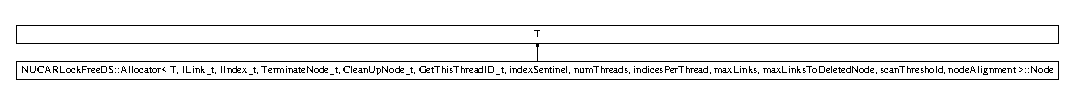
\includegraphics[height=0.841473cm]{class_n_u_c_a_r_lock_free_d_s_1_1_allocator_1_1_node}
\end{center}
\end{figure}
\subsection*{Public Member Functions}
\begin{DoxyCompactItemize}
\item 
\+\_\+\+\_\+device\+\_\+\+\_\+ \mbox{\hyperlink{class_n_u_c_a_r_lock_free_d_s_1_1_allocator_1_1_node_ac6eeee00317554695aed9e4657d222d7}{Node}} ()
\end{DoxyCompactItemize}
\subsection*{Private Attributes}
\begin{DoxyCompactItemize}
\item 
volatile int \mbox{\hyperlink{class_n_u_c_a_r_lock_free_d_s_1_1_allocator_1_1_node_a312678ef69212305fcb1a502487ecbf0}{ref\+Count}}
\item 
volatile bool \mbox{\hyperlink{class_n_u_c_a_r_lock_free_d_s_1_1_allocator_1_1_node_a2f124c812c1bff924eb839a4dcd372b8}{trace}}
\item 
volatile bool \mbox{\hyperlink{class_n_u_c_a_r_lock_free_d_s_1_1_allocator_1_1_node_ab5fd866eb1405eb7c5962f7842d6f546}{del}}
\end{DoxyCompactItemize}
\subsection*{Friends}
\begin{DoxyCompactItemize}
\item 
class \mbox{\hyperlink{class_n_u_c_a_r_lock_free_d_s_1_1_allocator_1_1_node_a4580c3239c67ddcfdafff4feae0d9b1d}{This\+\_\+t}}
\end{DoxyCompactItemize}


\subsection{Detailed Description}
\subsubsection*{template$<$typename T, typename I\+Link\+\_\+t, typename I\+Index\+\_\+t, typename Terminate\+Node\+\_\+t, typename Clean\+Up\+Node\+\_\+t, typename Get\+This\+Thread\+I\+D\+\_\+t, I\+Index\+\_\+t index\+Sentinel, I\+Index\+\_\+t num\+Threads, I\+Index\+\_\+t indices\+Per\+Thread, I\+Index\+\_\+t max\+Links, I\+Index\+\_\+t max\+Links\+To\+Deleted\+Node, I\+Index\+\_\+t scan\+Threshold, unsigned long long int node\+Alignment = 8$>$\newline
class N\+U\+C\+A\+R\+Lock\+Free\+D\+S\+::\+Allocator$<$ T, I\+Link\+\_\+t, I\+Index\+\_\+t, Terminate\+Node\+\_\+t, Clean\+Up\+Node\+\_\+t, Get\+This\+Thread\+I\+D\+\_\+t, index\+Sentinel, num\+Threads, indices\+Per\+Thread, max\+Links, max\+Links\+To\+Deleted\+Node, scan\+Threshold, node\+Alignment $>$\+::\+Node}

\mbox{\hyperlink{class_n_u_c_a_r_lock_free_d_s_1_1_allocator}{Allocator}} node type that extends the type to be allocated T with some metadata required by the allocator. Instances of this type are passed to client code and are expected to be returned to client code via Link\+\_\+t\+::\+Get\+Node() 

\subsection{Constructor \& Destructor Documentation}
\mbox{\Hypertarget{class_n_u_c_a_r_lock_free_d_s_1_1_allocator_1_1_node_ac6eeee00317554695aed9e4657d222d7}\label{class_n_u_c_a_r_lock_free_d_s_1_1_allocator_1_1_node_ac6eeee00317554695aed9e4657d222d7}} 
\index{N\+U\+C\+A\+R\+Lock\+Free\+D\+S\+::\+Allocator\+::\+Node@{N\+U\+C\+A\+R\+Lock\+Free\+D\+S\+::\+Allocator\+::\+Node}!Node@{Node}}
\index{Node@{Node}!N\+U\+C\+A\+R\+Lock\+Free\+D\+S\+::\+Allocator\+::\+Node@{N\+U\+C\+A\+R\+Lock\+Free\+D\+S\+::\+Allocator\+::\+Node}}
\subsubsection{\texorpdfstring{Node()}{Node()}}
{\footnotesize\ttfamily template$<$typename T, typename I\+Link\+\_\+t, typename I\+Index\+\_\+t, typename Terminate\+Node\+\_\+t, typename Clean\+Up\+Node\+\_\+t, typename Get\+This\+Thread\+I\+D\+\_\+t, I\+Index\+\_\+t index\+Sentinel, I\+Index\+\_\+t num\+Threads, I\+Index\+\_\+t indices\+Per\+Thread, I\+Index\+\_\+t max\+Links, I\+Index\+\_\+t max\+Links\+To\+Deleted\+Node, I\+Index\+\_\+t scan\+Threshold, unsigned long long int node\+Alignment = 8$>$ \\
\+\_\+\+\_\+device\+\_\+\+\_\+ \mbox{\hyperlink{class_n_u_c_a_r_lock_free_d_s_1_1_allocator}{N\+U\+C\+A\+R\+Lock\+Free\+D\+S\+::\+Allocator}}$<$ T, I\+Link\+\_\+t, I\+Index\+\_\+t, Terminate\+Node\+\_\+t, Clean\+Up\+Node\+\_\+t, Get\+This\+Thread\+I\+D\+\_\+t, index\+Sentinel, num\+Threads, indices\+Per\+Thread, max\+Links, max\+Links\+To\+Deleted\+Node, scan\+Threshold, node\+Alignment $>$\+::Node\+::\+Node (\begin{DoxyParamCaption}{ }\end{DoxyParamCaption})\hspace{0.3cm}{\ttfamily [inline]}}



\subsection{Friends And Related Function Documentation}
\mbox{\Hypertarget{class_n_u_c_a_r_lock_free_d_s_1_1_allocator_1_1_node_a4580c3239c67ddcfdafff4feae0d9b1d}\label{class_n_u_c_a_r_lock_free_d_s_1_1_allocator_1_1_node_a4580c3239c67ddcfdafff4feae0d9b1d}} 
\index{N\+U\+C\+A\+R\+Lock\+Free\+D\+S\+::\+Allocator\+::\+Node@{N\+U\+C\+A\+R\+Lock\+Free\+D\+S\+::\+Allocator\+::\+Node}!This\+\_\+t@{This\+\_\+t}}
\index{This\+\_\+t@{This\+\_\+t}!N\+U\+C\+A\+R\+Lock\+Free\+D\+S\+::\+Allocator\+::\+Node@{N\+U\+C\+A\+R\+Lock\+Free\+D\+S\+::\+Allocator\+::\+Node}}
\subsubsection{\texorpdfstring{This\+\_\+t}{This\_t}}
{\footnotesize\ttfamily template$<$typename T, typename I\+Link\+\_\+t, typename I\+Index\+\_\+t, typename Terminate\+Node\+\_\+t, typename Clean\+Up\+Node\+\_\+t, typename Get\+This\+Thread\+I\+D\+\_\+t, I\+Index\+\_\+t index\+Sentinel, I\+Index\+\_\+t num\+Threads, I\+Index\+\_\+t indices\+Per\+Thread, I\+Index\+\_\+t max\+Links, I\+Index\+\_\+t max\+Links\+To\+Deleted\+Node, I\+Index\+\_\+t scan\+Threshold, unsigned long long int node\+Alignment = 8$>$ \\
friend class \mbox{\hyperlink{class_n_u_c_a_r_lock_free_d_s_1_1_allocator_aa7636b4884545094b9532cc295604b17}{This\+\_\+t}}\hspace{0.3cm}{\ttfamily [friend]}}



\subsection{Member Data Documentation}
\mbox{\Hypertarget{class_n_u_c_a_r_lock_free_d_s_1_1_allocator_1_1_node_ab5fd866eb1405eb7c5962f7842d6f546}\label{class_n_u_c_a_r_lock_free_d_s_1_1_allocator_1_1_node_ab5fd866eb1405eb7c5962f7842d6f546}} 
\index{N\+U\+C\+A\+R\+Lock\+Free\+D\+S\+::\+Allocator\+::\+Node@{N\+U\+C\+A\+R\+Lock\+Free\+D\+S\+::\+Allocator\+::\+Node}!del@{del}}
\index{del@{del}!N\+U\+C\+A\+R\+Lock\+Free\+D\+S\+::\+Allocator\+::\+Node@{N\+U\+C\+A\+R\+Lock\+Free\+D\+S\+::\+Allocator\+::\+Node}}
\subsubsection{\texorpdfstring{del}{del}}
{\footnotesize\ttfamily template$<$typename T, typename I\+Link\+\_\+t, typename I\+Index\+\_\+t, typename Terminate\+Node\+\_\+t, typename Clean\+Up\+Node\+\_\+t, typename Get\+This\+Thread\+I\+D\+\_\+t, I\+Index\+\_\+t index\+Sentinel, I\+Index\+\_\+t num\+Threads, I\+Index\+\_\+t indices\+Per\+Thread, I\+Index\+\_\+t max\+Links, I\+Index\+\_\+t max\+Links\+To\+Deleted\+Node, I\+Index\+\_\+t scan\+Threshold, unsigned long long int node\+Alignment = 8$>$ \\
volatile bool \mbox{\hyperlink{class_n_u_c_a_r_lock_free_d_s_1_1_allocator}{N\+U\+C\+A\+R\+Lock\+Free\+D\+S\+::\+Allocator}}$<$ T, I\+Link\+\_\+t, I\+Index\+\_\+t, Terminate\+Node\+\_\+t, Clean\+Up\+Node\+\_\+t, Get\+This\+Thread\+I\+D\+\_\+t, index\+Sentinel, num\+Threads, indices\+Per\+Thread, max\+Links, max\+Links\+To\+Deleted\+Node, scan\+Threshold, node\+Alignment $>$\+::Node\+::del\hspace{0.3cm}{\ttfamily [private]}}

\mbox{\Hypertarget{class_n_u_c_a_r_lock_free_d_s_1_1_allocator_1_1_node_a312678ef69212305fcb1a502487ecbf0}\label{class_n_u_c_a_r_lock_free_d_s_1_1_allocator_1_1_node_a312678ef69212305fcb1a502487ecbf0}} 
\index{N\+U\+C\+A\+R\+Lock\+Free\+D\+S\+::\+Allocator\+::\+Node@{N\+U\+C\+A\+R\+Lock\+Free\+D\+S\+::\+Allocator\+::\+Node}!ref\+Count@{ref\+Count}}
\index{ref\+Count@{ref\+Count}!N\+U\+C\+A\+R\+Lock\+Free\+D\+S\+::\+Allocator\+::\+Node@{N\+U\+C\+A\+R\+Lock\+Free\+D\+S\+::\+Allocator\+::\+Node}}
\subsubsection{\texorpdfstring{ref\+Count}{refCount}}
{\footnotesize\ttfamily template$<$typename T, typename I\+Link\+\_\+t, typename I\+Index\+\_\+t, typename Terminate\+Node\+\_\+t, typename Clean\+Up\+Node\+\_\+t, typename Get\+This\+Thread\+I\+D\+\_\+t, I\+Index\+\_\+t index\+Sentinel, I\+Index\+\_\+t num\+Threads, I\+Index\+\_\+t indices\+Per\+Thread, I\+Index\+\_\+t max\+Links, I\+Index\+\_\+t max\+Links\+To\+Deleted\+Node, I\+Index\+\_\+t scan\+Threshold, unsigned long long int node\+Alignment = 8$>$ \\
volatile int \mbox{\hyperlink{class_n_u_c_a_r_lock_free_d_s_1_1_allocator}{N\+U\+C\+A\+R\+Lock\+Free\+D\+S\+::\+Allocator}}$<$ T, I\+Link\+\_\+t, I\+Index\+\_\+t, Terminate\+Node\+\_\+t, Clean\+Up\+Node\+\_\+t, Get\+This\+Thread\+I\+D\+\_\+t, index\+Sentinel, num\+Threads, indices\+Per\+Thread, max\+Links, max\+Links\+To\+Deleted\+Node, scan\+Threshold, node\+Alignment $>$\+::Node\+::ref\+Count\hspace{0.3cm}{\ttfamily [private]}}

\mbox{\Hypertarget{class_n_u_c_a_r_lock_free_d_s_1_1_allocator_1_1_node_a2f124c812c1bff924eb839a4dcd372b8}\label{class_n_u_c_a_r_lock_free_d_s_1_1_allocator_1_1_node_a2f124c812c1bff924eb839a4dcd372b8}} 
\index{N\+U\+C\+A\+R\+Lock\+Free\+D\+S\+::\+Allocator\+::\+Node@{N\+U\+C\+A\+R\+Lock\+Free\+D\+S\+::\+Allocator\+::\+Node}!trace@{trace}}
\index{trace@{trace}!N\+U\+C\+A\+R\+Lock\+Free\+D\+S\+::\+Allocator\+::\+Node@{N\+U\+C\+A\+R\+Lock\+Free\+D\+S\+::\+Allocator\+::\+Node}}
\subsubsection{\texorpdfstring{trace}{trace}}
{\footnotesize\ttfamily template$<$typename T, typename I\+Link\+\_\+t, typename I\+Index\+\_\+t, typename Terminate\+Node\+\_\+t, typename Clean\+Up\+Node\+\_\+t, typename Get\+This\+Thread\+I\+D\+\_\+t, I\+Index\+\_\+t index\+Sentinel, I\+Index\+\_\+t num\+Threads, I\+Index\+\_\+t indices\+Per\+Thread, I\+Index\+\_\+t max\+Links, I\+Index\+\_\+t max\+Links\+To\+Deleted\+Node, I\+Index\+\_\+t scan\+Threshold, unsigned long long int node\+Alignment = 8$>$ \\
volatile bool \mbox{\hyperlink{class_n_u_c_a_r_lock_free_d_s_1_1_allocator}{N\+U\+C\+A\+R\+Lock\+Free\+D\+S\+::\+Allocator}}$<$ T, I\+Link\+\_\+t, I\+Index\+\_\+t, Terminate\+Node\+\_\+t, Clean\+Up\+Node\+\_\+t, Get\+This\+Thread\+I\+D\+\_\+t, index\+Sentinel, num\+Threads, indices\+Per\+Thread, max\+Links, max\+Links\+To\+Deleted\+Node, scan\+Threshold, node\+Alignment $>$\+::Node\+::trace\hspace{0.3cm}{\ttfamily [private]}}



The documentation for this class was generated from the following file\+:\begin{DoxyCompactItemize}
\item 
G\+P\+U\+Lock\+Free\+Data\+Structures/\mbox{\hyperlink{_allocator_8hpp}{Allocator.\+hpp}}\end{DoxyCompactItemize}

\hypertarget{class_n_u_c_a_r_lock_free_d_s_1_1_allocator_1_1_per_thread_state}{}\section{N\+U\+C\+A\+R\+Lock\+Free\+DS\+:\+:Allocator$<$ T, I\+Link\+\_\+t, I\+Index\+\_\+t, Terminate\+Node\+\_\+t, Clean\+Up\+Node\+\_\+t, Get\+This\+Thread\+I\+D\+\_\+t, index\+Sentinel, num\+Threads, indices\+Per\+Thread, max\+Links, max\+Links\+To\+Deleted\+Node, scan\+Threshold, node\+Alignment $>$\+:\+:Per\+Thread\+State Class Reference}
\label{class_n_u_c_a_r_lock_free_d_s_1_1_allocator_1_1_per_thread_state}\index{N\+U\+C\+A\+R\+Lock\+Free\+D\+S\+::\+Allocator$<$ T, I\+Link\+\_\+t, I\+Index\+\_\+t, Terminate\+Node\+\_\+t, Clean\+Up\+Node\+\_\+t, Get\+This\+Thread\+I\+D\+\_\+t, index\+Sentinel, num\+Threads, indices\+Per\+Thread, max\+Links, max\+Links\+To\+Deleted\+Node, scan\+Threshold, node\+Alignment $>$\+::\+Per\+Thread\+State@{N\+U\+C\+A\+R\+Lock\+Free\+D\+S\+::\+Allocator$<$ T, I\+Link\+\_\+t, I\+Index\+\_\+t, Terminate\+Node\+\_\+t, Clean\+Up\+Node\+\_\+t, Get\+This\+Thread\+I\+D\+\_\+t, index\+Sentinel, num\+Threads, indices\+Per\+Thread, max\+Links, max\+Links\+To\+Deleted\+Node, scan\+Threshold, node\+Alignment $>$\+::\+Per\+Thread\+State}}
\subsection*{Public Member Functions}
\begin{DoxyCompactItemize}
\item 
\+\_\+\+\_\+device\+\_\+\+\_\+ \mbox{\hyperlink{class_n_u_c_a_r_lock_free_d_s_1_1_allocator_1_1_per_thread_state_ac2171d73e5b34d3a391d4f92802f8171}{Per\+Thread\+State}} ()
\end{DoxyCompactItemize}
\subsection*{Public Attributes}
\begin{DoxyCompactItemize}
\item 
\mbox{\hyperlink{class_n_u_c_a_r_lock_free_d_s_1_1_allocator_a2776cca35e8343bf5007bd8b6f3a3f8f}{Index\+\_\+t}} \mbox{\hyperlink{class_n_u_c_a_r_lock_free_d_s_1_1_allocator_1_1_per_thread_state_a70b267fa370752120e752af9651467d7}{dlist}}
\item 
\mbox{\hyperlink{class_n_u_c_a_r_lock_free_d_s_1_1_allocator_a2776cca35e8343bf5007bd8b6f3a3f8f}{Index\+\_\+t}} \mbox{\hyperlink{class_n_u_c_a_r_lock_free_d_s_1_1_allocator_1_1_per_thread_state_add29cc3216c93c4dbc5287dd5c296f07}{dcount}}
\item 
\mbox{\hyperlink{class_n_u_c_a_r_lock_free_d_s_1_1_allocator_a2776cca35e8343bf5007bd8b6f3a3f8f}{Index\+\_\+t}} \mbox{\hyperlink{class_n_u_c_a_r_lock_free_d_s_1_1_allocator_1_1_per_thread_state_acda67994c55201445540612f40ce4381}{D\+L\+Nexts}} \mbox{[}\mbox{\hyperlink{class_n_u_c_a_r_lock_free_d_s_1_1_allocator_a1d220e1cc963fc9fb37e46a416504715}{threshold1}}\mbox{]}
\item 
\mbox{\hyperlink{class_n_u_c_a_r_lock_free_d_s_1_1_allocator_1_1_p_list}{P\+List}} \mbox{\hyperlink{class_n_u_c_a_r_lock_free_d_s_1_1_allocator_1_1_per_thread_state_a034074390f23263717fea75eb0b814b5}{node\+List}}
\end{DoxyCompactItemize}


\subsection{Constructor \& Destructor Documentation}
\mbox{\Hypertarget{class_n_u_c_a_r_lock_free_d_s_1_1_allocator_1_1_per_thread_state_ac2171d73e5b34d3a391d4f92802f8171}\label{class_n_u_c_a_r_lock_free_d_s_1_1_allocator_1_1_per_thread_state_ac2171d73e5b34d3a391d4f92802f8171}} 
\index{N\+U\+C\+A\+R\+Lock\+Free\+D\+S\+::\+Allocator\+::\+Per\+Thread\+State@{N\+U\+C\+A\+R\+Lock\+Free\+D\+S\+::\+Allocator\+::\+Per\+Thread\+State}!Per\+Thread\+State@{Per\+Thread\+State}}
\index{Per\+Thread\+State@{Per\+Thread\+State}!N\+U\+C\+A\+R\+Lock\+Free\+D\+S\+::\+Allocator\+::\+Per\+Thread\+State@{N\+U\+C\+A\+R\+Lock\+Free\+D\+S\+::\+Allocator\+::\+Per\+Thread\+State}}
\subsubsection{\texorpdfstring{Per\+Thread\+State()}{PerThreadState()}}
{\footnotesize\ttfamily template$<$typename T, typename I\+Link\+\_\+t, typename I\+Index\+\_\+t, typename Terminate\+Node\+\_\+t, typename Clean\+Up\+Node\+\_\+t, typename Get\+This\+Thread\+I\+D\+\_\+t, I\+Index\+\_\+t index\+Sentinel, I\+Index\+\_\+t num\+Threads, I\+Index\+\_\+t indices\+Per\+Thread, I\+Index\+\_\+t max\+Links, I\+Index\+\_\+t max\+Links\+To\+Deleted\+Node, I\+Index\+\_\+t scan\+Threshold, unsigned long long int node\+Alignment = 8$>$ \\
\+\_\+\+\_\+device\+\_\+\+\_\+ \mbox{\hyperlink{class_n_u_c_a_r_lock_free_d_s_1_1_allocator}{N\+U\+C\+A\+R\+Lock\+Free\+D\+S\+::\+Allocator}}$<$ T, I\+Link\+\_\+t, I\+Index\+\_\+t, Terminate\+Node\+\_\+t, Clean\+Up\+Node\+\_\+t, Get\+This\+Thread\+I\+D\+\_\+t, index\+Sentinel, num\+Threads, indices\+Per\+Thread, max\+Links, max\+Links\+To\+Deleted\+Node, scan\+Threshold, node\+Alignment $>$\+::Per\+Thread\+State\+::\+Per\+Thread\+State (\begin{DoxyParamCaption}{ }\end{DoxyParamCaption})\hspace{0.3cm}{\ttfamily [inline]}}



\subsection{Member Data Documentation}
\mbox{\Hypertarget{class_n_u_c_a_r_lock_free_d_s_1_1_allocator_1_1_per_thread_state_add29cc3216c93c4dbc5287dd5c296f07}\label{class_n_u_c_a_r_lock_free_d_s_1_1_allocator_1_1_per_thread_state_add29cc3216c93c4dbc5287dd5c296f07}} 
\index{N\+U\+C\+A\+R\+Lock\+Free\+D\+S\+::\+Allocator\+::\+Per\+Thread\+State@{N\+U\+C\+A\+R\+Lock\+Free\+D\+S\+::\+Allocator\+::\+Per\+Thread\+State}!dcount@{dcount}}
\index{dcount@{dcount}!N\+U\+C\+A\+R\+Lock\+Free\+D\+S\+::\+Allocator\+::\+Per\+Thread\+State@{N\+U\+C\+A\+R\+Lock\+Free\+D\+S\+::\+Allocator\+::\+Per\+Thread\+State}}
\subsubsection{\texorpdfstring{dcount}{dcount}}
{\footnotesize\ttfamily template$<$typename T, typename I\+Link\+\_\+t, typename I\+Index\+\_\+t, typename Terminate\+Node\+\_\+t, typename Clean\+Up\+Node\+\_\+t, typename Get\+This\+Thread\+I\+D\+\_\+t, I\+Index\+\_\+t index\+Sentinel, I\+Index\+\_\+t num\+Threads, I\+Index\+\_\+t indices\+Per\+Thread, I\+Index\+\_\+t max\+Links, I\+Index\+\_\+t max\+Links\+To\+Deleted\+Node, I\+Index\+\_\+t scan\+Threshold, unsigned long long int node\+Alignment = 8$>$ \\
\mbox{\hyperlink{class_n_u_c_a_r_lock_free_d_s_1_1_allocator_a2776cca35e8343bf5007bd8b6f3a3f8f}{Index\+\_\+t}} \mbox{\hyperlink{class_n_u_c_a_r_lock_free_d_s_1_1_allocator}{N\+U\+C\+A\+R\+Lock\+Free\+D\+S\+::\+Allocator}}$<$ T, I\+Link\+\_\+t, I\+Index\+\_\+t, Terminate\+Node\+\_\+t, Clean\+Up\+Node\+\_\+t, Get\+This\+Thread\+I\+D\+\_\+t, index\+Sentinel, num\+Threads, indices\+Per\+Thread, max\+Links, max\+Links\+To\+Deleted\+Node, scan\+Threshold, node\+Alignment $>$\+::Per\+Thread\+State\+::dcount}

\mbox{\Hypertarget{class_n_u_c_a_r_lock_free_d_s_1_1_allocator_1_1_per_thread_state_a70b267fa370752120e752af9651467d7}\label{class_n_u_c_a_r_lock_free_d_s_1_1_allocator_1_1_per_thread_state_a70b267fa370752120e752af9651467d7}} 
\index{N\+U\+C\+A\+R\+Lock\+Free\+D\+S\+::\+Allocator\+::\+Per\+Thread\+State@{N\+U\+C\+A\+R\+Lock\+Free\+D\+S\+::\+Allocator\+::\+Per\+Thread\+State}!dlist@{dlist}}
\index{dlist@{dlist}!N\+U\+C\+A\+R\+Lock\+Free\+D\+S\+::\+Allocator\+::\+Per\+Thread\+State@{N\+U\+C\+A\+R\+Lock\+Free\+D\+S\+::\+Allocator\+::\+Per\+Thread\+State}}
\subsubsection{\texorpdfstring{dlist}{dlist}}
{\footnotesize\ttfamily template$<$typename T, typename I\+Link\+\_\+t, typename I\+Index\+\_\+t, typename Terminate\+Node\+\_\+t, typename Clean\+Up\+Node\+\_\+t, typename Get\+This\+Thread\+I\+D\+\_\+t, I\+Index\+\_\+t index\+Sentinel, I\+Index\+\_\+t num\+Threads, I\+Index\+\_\+t indices\+Per\+Thread, I\+Index\+\_\+t max\+Links, I\+Index\+\_\+t max\+Links\+To\+Deleted\+Node, I\+Index\+\_\+t scan\+Threshold, unsigned long long int node\+Alignment = 8$>$ \\
\mbox{\hyperlink{class_n_u_c_a_r_lock_free_d_s_1_1_allocator_a2776cca35e8343bf5007bd8b6f3a3f8f}{Index\+\_\+t}} \mbox{\hyperlink{class_n_u_c_a_r_lock_free_d_s_1_1_allocator}{N\+U\+C\+A\+R\+Lock\+Free\+D\+S\+::\+Allocator}}$<$ T, I\+Link\+\_\+t, I\+Index\+\_\+t, Terminate\+Node\+\_\+t, Clean\+Up\+Node\+\_\+t, Get\+This\+Thread\+I\+D\+\_\+t, index\+Sentinel, num\+Threads, indices\+Per\+Thread, max\+Links, max\+Links\+To\+Deleted\+Node, scan\+Threshold, node\+Alignment $>$\+::Per\+Thread\+State\+::dlist}

\mbox{\Hypertarget{class_n_u_c_a_r_lock_free_d_s_1_1_allocator_1_1_per_thread_state_acda67994c55201445540612f40ce4381}\label{class_n_u_c_a_r_lock_free_d_s_1_1_allocator_1_1_per_thread_state_acda67994c55201445540612f40ce4381}} 
\index{N\+U\+C\+A\+R\+Lock\+Free\+D\+S\+::\+Allocator\+::\+Per\+Thread\+State@{N\+U\+C\+A\+R\+Lock\+Free\+D\+S\+::\+Allocator\+::\+Per\+Thread\+State}!D\+L\+Nexts@{D\+L\+Nexts}}
\index{D\+L\+Nexts@{D\+L\+Nexts}!N\+U\+C\+A\+R\+Lock\+Free\+D\+S\+::\+Allocator\+::\+Per\+Thread\+State@{N\+U\+C\+A\+R\+Lock\+Free\+D\+S\+::\+Allocator\+::\+Per\+Thread\+State}}
\subsubsection{\texorpdfstring{D\+L\+Nexts}{DLNexts}}
{\footnotesize\ttfamily template$<$typename T, typename I\+Link\+\_\+t, typename I\+Index\+\_\+t, typename Terminate\+Node\+\_\+t, typename Clean\+Up\+Node\+\_\+t, typename Get\+This\+Thread\+I\+D\+\_\+t, I\+Index\+\_\+t index\+Sentinel, I\+Index\+\_\+t num\+Threads, I\+Index\+\_\+t indices\+Per\+Thread, I\+Index\+\_\+t max\+Links, I\+Index\+\_\+t max\+Links\+To\+Deleted\+Node, I\+Index\+\_\+t scan\+Threshold, unsigned long long int node\+Alignment = 8$>$ \\
\mbox{\hyperlink{class_n_u_c_a_r_lock_free_d_s_1_1_allocator_a2776cca35e8343bf5007bd8b6f3a3f8f}{Index\+\_\+t}} \mbox{\hyperlink{class_n_u_c_a_r_lock_free_d_s_1_1_allocator}{N\+U\+C\+A\+R\+Lock\+Free\+D\+S\+::\+Allocator}}$<$ T, I\+Link\+\_\+t, I\+Index\+\_\+t, Terminate\+Node\+\_\+t, Clean\+Up\+Node\+\_\+t, Get\+This\+Thread\+I\+D\+\_\+t, index\+Sentinel, num\+Threads, indices\+Per\+Thread, max\+Links, max\+Links\+To\+Deleted\+Node, scan\+Threshold, node\+Alignment $>$\+::Per\+Thread\+State\+::\+D\+L\+Nexts\mbox{[}\mbox{\hyperlink{class_n_u_c_a_r_lock_free_d_s_1_1_allocator_a1d220e1cc963fc9fb37e46a416504715}{threshold1}}\mbox{]}}

\mbox{\Hypertarget{class_n_u_c_a_r_lock_free_d_s_1_1_allocator_1_1_per_thread_state_a034074390f23263717fea75eb0b814b5}\label{class_n_u_c_a_r_lock_free_d_s_1_1_allocator_1_1_per_thread_state_a034074390f23263717fea75eb0b814b5}} 
\index{N\+U\+C\+A\+R\+Lock\+Free\+D\+S\+::\+Allocator\+::\+Per\+Thread\+State@{N\+U\+C\+A\+R\+Lock\+Free\+D\+S\+::\+Allocator\+::\+Per\+Thread\+State}!node\+List@{node\+List}}
\index{node\+List@{node\+List}!N\+U\+C\+A\+R\+Lock\+Free\+D\+S\+::\+Allocator\+::\+Per\+Thread\+State@{N\+U\+C\+A\+R\+Lock\+Free\+D\+S\+::\+Allocator\+::\+Per\+Thread\+State}}
\subsubsection{\texorpdfstring{node\+List}{nodeList}}
{\footnotesize\ttfamily template$<$typename T, typename I\+Link\+\_\+t, typename I\+Index\+\_\+t, typename Terminate\+Node\+\_\+t, typename Clean\+Up\+Node\+\_\+t, typename Get\+This\+Thread\+I\+D\+\_\+t, I\+Index\+\_\+t index\+Sentinel, I\+Index\+\_\+t num\+Threads, I\+Index\+\_\+t indices\+Per\+Thread, I\+Index\+\_\+t max\+Links, I\+Index\+\_\+t max\+Links\+To\+Deleted\+Node, I\+Index\+\_\+t scan\+Threshold, unsigned long long int node\+Alignment = 8$>$ \\
\mbox{\hyperlink{class_n_u_c_a_r_lock_free_d_s_1_1_allocator_1_1_p_list}{P\+List}} \mbox{\hyperlink{class_n_u_c_a_r_lock_free_d_s_1_1_allocator}{N\+U\+C\+A\+R\+Lock\+Free\+D\+S\+::\+Allocator}}$<$ T, I\+Link\+\_\+t, I\+Index\+\_\+t, Terminate\+Node\+\_\+t, Clean\+Up\+Node\+\_\+t, Get\+This\+Thread\+I\+D\+\_\+t, index\+Sentinel, num\+Threads, indices\+Per\+Thread, max\+Links, max\+Links\+To\+Deleted\+Node, scan\+Threshold, node\+Alignment $>$\+::Per\+Thread\+State\+::node\+List}



The documentation for this class was generated from the following file\+:\begin{DoxyCompactItemize}
\item 
G\+P\+U\+Lock\+Free\+Data\+Structures/\mbox{\hyperlink{_allocator_8hpp}{Allocator.\+hpp}}\end{DoxyCompactItemize}

\hypertarget{class_n_u_c_a_r_lock_free_d_s_1_1_allocator_1_1_p_list}{}\section{N\+U\+C\+A\+R\+Lock\+Free\+DS\+:\+:Allocator$<$ T, I\+Link\+\_\+t, I\+Index\+\_\+t, Terminate\+Node\+\_\+t, Clean\+Up\+Node\+\_\+t, Get\+This\+Thread\+I\+D\+\_\+t, index\+Sentinel, num\+Threads, indices\+Per\+Thread, max\+Links, max\+Links\+To\+Deleted\+Node, scan\+Threshold, node\+Alignment $>$\+:\+:P\+List Class Reference}
\label{class_n_u_c_a_r_lock_free_d_s_1_1_allocator_1_1_p_list}\index{N\+U\+C\+A\+R\+Lock\+Free\+D\+S\+::\+Allocator$<$ T, I\+Link\+\_\+t, I\+Index\+\_\+t, Terminate\+Node\+\_\+t, Clean\+Up\+Node\+\_\+t, Get\+This\+Thread\+I\+D\+\_\+t, index\+Sentinel, num\+Threads, indices\+Per\+Thread, max\+Links, max\+Links\+To\+Deleted\+Node, scan\+Threshold, node\+Alignment $>$\+::\+P\+List@{N\+U\+C\+A\+R\+Lock\+Free\+D\+S\+::\+Allocator$<$ T, I\+Link\+\_\+t, I\+Index\+\_\+t, Terminate\+Node\+\_\+t, Clean\+Up\+Node\+\_\+t, Get\+This\+Thread\+I\+D\+\_\+t, index\+Sentinel, num\+Threads, indices\+Per\+Thread, max\+Links, max\+Links\+To\+Deleted\+Node, scan\+Threshold, node\+Alignment $>$\+::\+P\+List}}
\subsection*{Public Member Functions}
\begin{DoxyCompactItemize}
\item 
\+\_\+\+\_\+device\+\_\+\+\_\+ void \mbox{\hyperlink{class_n_u_c_a_r_lock_free_d_s_1_1_allocator_1_1_p_list_a62645ee0694885ea2d460db3c34c84ae}{add\+Node}} (const \mbox{\hyperlink{class_n_u_c_a_r_lock_free_d_s_1_1_allocator_1_1_node}{Node}} $\ast$data)
\item 
\+\_\+\+\_\+device\+\_\+\+\_\+ bool \mbox{\hyperlink{class_n_u_c_a_r_lock_free_d_s_1_1_allocator_1_1_p_list_a7131962e802f28f5bf5220211c7f5eb8}{contains}} (const \mbox{\hyperlink{class_n_u_c_a_r_lock_free_d_s_1_1_allocator_1_1_node}{Node}} $\ast$elem)
\item 
\+\_\+\+\_\+device\+\_\+\+\_\+ void \mbox{\hyperlink{class_n_u_c_a_r_lock_free_d_s_1_1_allocator_1_1_p_list_a05e00c2ca0f24298e7db21563368a416}{clear}} ()
\item 
\+\_\+\+\_\+device\+\_\+\+\_\+ \mbox{\hyperlink{class_n_u_c_a_r_lock_free_d_s_1_1_allocator_1_1_p_list_afd02db15ba9865760bb8c0649c1897a7}{P\+List}} ()
\end{DoxyCompactItemize}
\subsection*{Private Attributes}
\begin{DoxyCompactItemize}
\item 
\mbox{\hyperlink{class_n_u_c_a_r_lock_free_d_s_1_1_allocator_1_1_node}{Node}} const  $\ast$ \mbox{\hyperlink{class_n_u_c_a_r_lock_free_d_s_1_1_allocator_1_1_p_list_ac90fa5d4c7048415d16c8b46e5b3290a}{storage}} \mbox{[}num\+Threads $\ast$indices\+Per\+Thread\mbox{]}
\item 
\mbox{\hyperlink{class_n_u_c_a_r_lock_free_d_s_1_1_allocator_a2776cca35e8343bf5007bd8b6f3a3f8f}{Index\+\_\+t}} \mbox{\hyperlink{class_n_u_c_a_r_lock_free_d_s_1_1_allocator_1_1_p_list_a36446eb7ee5bc5173b9877e3baa9a3a4}{position}}
\end{DoxyCompactItemize}


\subsection{Constructor \& Destructor Documentation}
\mbox{\Hypertarget{class_n_u_c_a_r_lock_free_d_s_1_1_allocator_1_1_p_list_afd02db15ba9865760bb8c0649c1897a7}\label{class_n_u_c_a_r_lock_free_d_s_1_1_allocator_1_1_p_list_afd02db15ba9865760bb8c0649c1897a7}} 
\index{N\+U\+C\+A\+R\+Lock\+Free\+D\+S\+::\+Allocator\+::\+P\+List@{N\+U\+C\+A\+R\+Lock\+Free\+D\+S\+::\+Allocator\+::\+P\+List}!P\+List@{P\+List}}
\index{P\+List@{P\+List}!N\+U\+C\+A\+R\+Lock\+Free\+D\+S\+::\+Allocator\+::\+P\+List@{N\+U\+C\+A\+R\+Lock\+Free\+D\+S\+::\+Allocator\+::\+P\+List}}
\subsubsection{\texorpdfstring{P\+List()}{PList()}}
{\footnotesize\ttfamily template$<$typename T, typename I\+Link\+\_\+t, typename I\+Index\+\_\+t, typename Terminate\+Node\+\_\+t, typename Clean\+Up\+Node\+\_\+t, typename Get\+This\+Thread\+I\+D\+\_\+t, I\+Index\+\_\+t index\+Sentinel, I\+Index\+\_\+t num\+Threads, I\+Index\+\_\+t indices\+Per\+Thread, I\+Index\+\_\+t max\+Links, I\+Index\+\_\+t max\+Links\+To\+Deleted\+Node, I\+Index\+\_\+t scan\+Threshold, unsigned long long int node\+Alignment = 8$>$ \\
\+\_\+\+\_\+device\+\_\+\+\_\+ \mbox{\hyperlink{class_n_u_c_a_r_lock_free_d_s_1_1_allocator}{N\+U\+C\+A\+R\+Lock\+Free\+D\+S\+::\+Allocator}}$<$ T, I\+Link\+\_\+t, I\+Index\+\_\+t, Terminate\+Node\+\_\+t, Clean\+Up\+Node\+\_\+t, Get\+This\+Thread\+I\+D\+\_\+t, index\+Sentinel, num\+Threads, indices\+Per\+Thread, max\+Links, max\+Links\+To\+Deleted\+Node, scan\+Threshold, node\+Alignment $>$\+::P\+List\+::\+P\+List (\begin{DoxyParamCaption}{ }\end{DoxyParamCaption})\hspace{0.3cm}{\ttfamily [inline]}}



\subsection{Member Function Documentation}
\mbox{\Hypertarget{class_n_u_c_a_r_lock_free_d_s_1_1_allocator_1_1_p_list_a62645ee0694885ea2d460db3c34c84ae}\label{class_n_u_c_a_r_lock_free_d_s_1_1_allocator_1_1_p_list_a62645ee0694885ea2d460db3c34c84ae}} 
\index{N\+U\+C\+A\+R\+Lock\+Free\+D\+S\+::\+Allocator\+::\+P\+List@{N\+U\+C\+A\+R\+Lock\+Free\+D\+S\+::\+Allocator\+::\+P\+List}!add\+Node@{add\+Node}}
\index{add\+Node@{add\+Node}!N\+U\+C\+A\+R\+Lock\+Free\+D\+S\+::\+Allocator\+::\+P\+List@{N\+U\+C\+A\+R\+Lock\+Free\+D\+S\+::\+Allocator\+::\+P\+List}}
\subsubsection{\texorpdfstring{add\+Node()}{addNode()}}
{\footnotesize\ttfamily template$<$typename T, typename I\+Link\+\_\+t, typename I\+Index\+\_\+t, typename Terminate\+Node\+\_\+t, typename Clean\+Up\+Node\+\_\+t, typename Get\+This\+Thread\+I\+D\+\_\+t, I\+Index\+\_\+t index\+Sentinel, I\+Index\+\_\+t num\+Threads, I\+Index\+\_\+t indices\+Per\+Thread, I\+Index\+\_\+t max\+Links, I\+Index\+\_\+t max\+Links\+To\+Deleted\+Node, I\+Index\+\_\+t scan\+Threshold, unsigned long long int node\+Alignment = 8$>$ \\
\+\_\+\+\_\+device\+\_\+\+\_\+ void \mbox{\hyperlink{class_n_u_c_a_r_lock_free_d_s_1_1_allocator}{N\+U\+C\+A\+R\+Lock\+Free\+D\+S\+::\+Allocator}}$<$ T, I\+Link\+\_\+t, I\+Index\+\_\+t, Terminate\+Node\+\_\+t, Clean\+Up\+Node\+\_\+t, Get\+This\+Thread\+I\+D\+\_\+t, index\+Sentinel, num\+Threads, indices\+Per\+Thread, max\+Links, max\+Links\+To\+Deleted\+Node, scan\+Threshold, node\+Alignment $>$\+::P\+List\+::add\+Node (\begin{DoxyParamCaption}\item[{const \mbox{\hyperlink{class_n_u_c_a_r_lock_free_d_s_1_1_allocator_1_1_node}{Node}} $\ast$}]{data }\end{DoxyParamCaption})\hspace{0.3cm}{\ttfamily [inline]}}

\mbox{\Hypertarget{class_n_u_c_a_r_lock_free_d_s_1_1_allocator_1_1_p_list_a05e00c2ca0f24298e7db21563368a416}\label{class_n_u_c_a_r_lock_free_d_s_1_1_allocator_1_1_p_list_a05e00c2ca0f24298e7db21563368a416}} 
\index{N\+U\+C\+A\+R\+Lock\+Free\+D\+S\+::\+Allocator\+::\+P\+List@{N\+U\+C\+A\+R\+Lock\+Free\+D\+S\+::\+Allocator\+::\+P\+List}!clear@{clear}}
\index{clear@{clear}!N\+U\+C\+A\+R\+Lock\+Free\+D\+S\+::\+Allocator\+::\+P\+List@{N\+U\+C\+A\+R\+Lock\+Free\+D\+S\+::\+Allocator\+::\+P\+List}}
\subsubsection{\texorpdfstring{clear()}{clear()}}
{\footnotesize\ttfamily template$<$typename T, typename I\+Link\+\_\+t, typename I\+Index\+\_\+t, typename Terminate\+Node\+\_\+t, typename Clean\+Up\+Node\+\_\+t, typename Get\+This\+Thread\+I\+D\+\_\+t, I\+Index\+\_\+t index\+Sentinel, I\+Index\+\_\+t num\+Threads, I\+Index\+\_\+t indices\+Per\+Thread, I\+Index\+\_\+t max\+Links, I\+Index\+\_\+t max\+Links\+To\+Deleted\+Node, I\+Index\+\_\+t scan\+Threshold, unsigned long long int node\+Alignment = 8$>$ \\
\+\_\+\+\_\+device\+\_\+\+\_\+ void \mbox{\hyperlink{class_n_u_c_a_r_lock_free_d_s_1_1_allocator}{N\+U\+C\+A\+R\+Lock\+Free\+D\+S\+::\+Allocator}}$<$ T, I\+Link\+\_\+t, I\+Index\+\_\+t, Terminate\+Node\+\_\+t, Clean\+Up\+Node\+\_\+t, Get\+This\+Thread\+I\+D\+\_\+t, index\+Sentinel, num\+Threads, indices\+Per\+Thread, max\+Links, max\+Links\+To\+Deleted\+Node, scan\+Threshold, node\+Alignment $>$\+::P\+List\+::clear (\begin{DoxyParamCaption}{ }\end{DoxyParamCaption})\hspace{0.3cm}{\ttfamily [inline]}}

\mbox{\Hypertarget{class_n_u_c_a_r_lock_free_d_s_1_1_allocator_1_1_p_list_a7131962e802f28f5bf5220211c7f5eb8}\label{class_n_u_c_a_r_lock_free_d_s_1_1_allocator_1_1_p_list_a7131962e802f28f5bf5220211c7f5eb8}} 
\index{N\+U\+C\+A\+R\+Lock\+Free\+D\+S\+::\+Allocator\+::\+P\+List@{N\+U\+C\+A\+R\+Lock\+Free\+D\+S\+::\+Allocator\+::\+P\+List}!contains@{contains}}
\index{contains@{contains}!N\+U\+C\+A\+R\+Lock\+Free\+D\+S\+::\+Allocator\+::\+P\+List@{N\+U\+C\+A\+R\+Lock\+Free\+D\+S\+::\+Allocator\+::\+P\+List}}
\subsubsection{\texorpdfstring{contains()}{contains()}}
{\footnotesize\ttfamily template$<$typename T, typename I\+Link\+\_\+t, typename I\+Index\+\_\+t, typename Terminate\+Node\+\_\+t, typename Clean\+Up\+Node\+\_\+t, typename Get\+This\+Thread\+I\+D\+\_\+t, I\+Index\+\_\+t index\+Sentinel, I\+Index\+\_\+t num\+Threads, I\+Index\+\_\+t indices\+Per\+Thread, I\+Index\+\_\+t max\+Links, I\+Index\+\_\+t max\+Links\+To\+Deleted\+Node, I\+Index\+\_\+t scan\+Threshold, unsigned long long int node\+Alignment = 8$>$ \\
\+\_\+\+\_\+device\+\_\+\+\_\+ bool \mbox{\hyperlink{class_n_u_c_a_r_lock_free_d_s_1_1_allocator}{N\+U\+C\+A\+R\+Lock\+Free\+D\+S\+::\+Allocator}}$<$ T, I\+Link\+\_\+t, I\+Index\+\_\+t, Terminate\+Node\+\_\+t, Clean\+Up\+Node\+\_\+t, Get\+This\+Thread\+I\+D\+\_\+t, index\+Sentinel, num\+Threads, indices\+Per\+Thread, max\+Links, max\+Links\+To\+Deleted\+Node, scan\+Threshold, node\+Alignment $>$\+::P\+List\+::contains (\begin{DoxyParamCaption}\item[{const \mbox{\hyperlink{class_n_u_c_a_r_lock_free_d_s_1_1_allocator_1_1_node}{Node}} $\ast$}]{elem }\end{DoxyParamCaption})\hspace{0.3cm}{\ttfamily [inline]}}



\subsection{Member Data Documentation}
\mbox{\Hypertarget{class_n_u_c_a_r_lock_free_d_s_1_1_allocator_1_1_p_list_a36446eb7ee5bc5173b9877e3baa9a3a4}\label{class_n_u_c_a_r_lock_free_d_s_1_1_allocator_1_1_p_list_a36446eb7ee5bc5173b9877e3baa9a3a4}} 
\index{N\+U\+C\+A\+R\+Lock\+Free\+D\+S\+::\+Allocator\+::\+P\+List@{N\+U\+C\+A\+R\+Lock\+Free\+D\+S\+::\+Allocator\+::\+P\+List}!position@{position}}
\index{position@{position}!N\+U\+C\+A\+R\+Lock\+Free\+D\+S\+::\+Allocator\+::\+P\+List@{N\+U\+C\+A\+R\+Lock\+Free\+D\+S\+::\+Allocator\+::\+P\+List}}
\subsubsection{\texorpdfstring{position}{position}}
{\footnotesize\ttfamily template$<$typename T, typename I\+Link\+\_\+t, typename I\+Index\+\_\+t, typename Terminate\+Node\+\_\+t, typename Clean\+Up\+Node\+\_\+t, typename Get\+This\+Thread\+I\+D\+\_\+t, I\+Index\+\_\+t index\+Sentinel, I\+Index\+\_\+t num\+Threads, I\+Index\+\_\+t indices\+Per\+Thread, I\+Index\+\_\+t max\+Links, I\+Index\+\_\+t max\+Links\+To\+Deleted\+Node, I\+Index\+\_\+t scan\+Threshold, unsigned long long int node\+Alignment = 8$>$ \\
\mbox{\hyperlink{class_n_u_c_a_r_lock_free_d_s_1_1_allocator_a2776cca35e8343bf5007bd8b6f3a3f8f}{Index\+\_\+t}} \mbox{\hyperlink{class_n_u_c_a_r_lock_free_d_s_1_1_allocator}{N\+U\+C\+A\+R\+Lock\+Free\+D\+S\+::\+Allocator}}$<$ T, I\+Link\+\_\+t, I\+Index\+\_\+t, Terminate\+Node\+\_\+t, Clean\+Up\+Node\+\_\+t, Get\+This\+Thread\+I\+D\+\_\+t, index\+Sentinel, num\+Threads, indices\+Per\+Thread, max\+Links, max\+Links\+To\+Deleted\+Node, scan\+Threshold, node\+Alignment $>$\+::P\+List\+::position\hspace{0.3cm}{\ttfamily [private]}}

\mbox{\Hypertarget{class_n_u_c_a_r_lock_free_d_s_1_1_allocator_1_1_p_list_ac90fa5d4c7048415d16c8b46e5b3290a}\label{class_n_u_c_a_r_lock_free_d_s_1_1_allocator_1_1_p_list_ac90fa5d4c7048415d16c8b46e5b3290a}} 
\index{N\+U\+C\+A\+R\+Lock\+Free\+D\+S\+::\+Allocator\+::\+P\+List@{N\+U\+C\+A\+R\+Lock\+Free\+D\+S\+::\+Allocator\+::\+P\+List}!storage@{storage}}
\index{storage@{storage}!N\+U\+C\+A\+R\+Lock\+Free\+D\+S\+::\+Allocator\+::\+P\+List@{N\+U\+C\+A\+R\+Lock\+Free\+D\+S\+::\+Allocator\+::\+P\+List}}
\subsubsection{\texorpdfstring{storage}{storage}}
{\footnotesize\ttfamily template$<$typename T, typename I\+Link\+\_\+t, typename I\+Index\+\_\+t, typename Terminate\+Node\+\_\+t, typename Clean\+Up\+Node\+\_\+t, typename Get\+This\+Thread\+I\+D\+\_\+t, I\+Index\+\_\+t index\+Sentinel, I\+Index\+\_\+t num\+Threads, I\+Index\+\_\+t indices\+Per\+Thread, I\+Index\+\_\+t max\+Links, I\+Index\+\_\+t max\+Links\+To\+Deleted\+Node, I\+Index\+\_\+t scan\+Threshold, unsigned long long int node\+Alignment = 8$>$ \\
\mbox{\hyperlink{class_n_u_c_a_r_lock_free_d_s_1_1_allocator_1_1_node}{Node}} const$\ast$ \mbox{\hyperlink{class_n_u_c_a_r_lock_free_d_s_1_1_allocator}{N\+U\+C\+A\+R\+Lock\+Free\+D\+S\+::\+Allocator}}$<$ T, I\+Link\+\_\+t, I\+Index\+\_\+t, Terminate\+Node\+\_\+t, Clean\+Up\+Node\+\_\+t, Get\+This\+Thread\+I\+D\+\_\+t, index\+Sentinel, num\+Threads, indices\+Per\+Thread, max\+Links, max\+Links\+To\+Deleted\+Node, scan\+Threshold, node\+Alignment $>$\+::P\+List\+::storage\mbox{[}num\+Threads $\ast$indices\+Per\+Thread\mbox{]}\hspace{0.3cm}{\ttfamily [private]}}



The documentation for this class was generated from the following file\+:\begin{DoxyCompactItemize}
\item 
G\+P\+U\+Lock\+Free\+Data\+Structures/\mbox{\hyperlink{_allocator_8hpp}{Allocator.\+hpp}}\end{DoxyCompactItemize}

\hypertarget{class_lock_free_queue_g_p_u_1_1_lock_free_queue_1_1_queue_node}{}\section{Lock\+Free\+Queue\+G\+PU\+:\+:Lock\+Free\+Queue$<$ T, sentinel $>$\+:\+:Queue\+Node Class Reference}
\label{class_lock_free_queue_g_p_u_1_1_lock_free_queue_1_1_queue_node}\index{Lock\+Free\+Queue\+G\+P\+U\+::\+Lock\+Free\+Queue$<$ T, sentinel $>$\+::\+Queue\+Node@{Lock\+Free\+Queue\+G\+P\+U\+::\+Lock\+Free\+Queue$<$ T, sentinel $>$\+::\+Queue\+Node}}
\subsection*{Public Member Functions}
\begin{DoxyCompactItemize}
\item 
\+\_\+\+\_\+device\+\_\+\+\_\+ \mbox{\hyperlink{class_lock_free_queue_g_p_u_1_1_lock_free_queue_1_1_queue_node_a095b63d0a28cb181c784b61459bcfb25}{Queue\+Node}} (const T \&init\+Data)
\end{DoxyCompactItemize}
\subsection*{Public Attributes}
\begin{DoxyCompactItemize}
\item 
\mbox{\hyperlink{class_lock_free_queue_g_p_u_1_1_lock_free_queue_1_1_queue_node_pointer}{Queue\+Node\+Pointer}} \mbox{\hyperlink{class_lock_free_queue_g_p_u_1_1_lock_free_queue_1_1_queue_node_a3379b81218c1e1ec97169bf3dfa95cf6}{next}}
\item 
const T \mbox{\hyperlink{class_lock_free_queue_g_p_u_1_1_lock_free_queue_1_1_queue_node_a2cab98d8849b74f13f2241b954477435}{value}}
\end{DoxyCompactItemize}


\subsection{Constructor \& Destructor Documentation}
\mbox{\Hypertarget{class_lock_free_queue_g_p_u_1_1_lock_free_queue_1_1_queue_node_a095b63d0a28cb181c784b61459bcfb25}\label{class_lock_free_queue_g_p_u_1_1_lock_free_queue_1_1_queue_node_a095b63d0a28cb181c784b61459bcfb25}} 
\index{Lock\+Free\+Queue\+G\+P\+U\+::\+Lock\+Free\+Queue\+::\+Queue\+Node@{Lock\+Free\+Queue\+G\+P\+U\+::\+Lock\+Free\+Queue\+::\+Queue\+Node}!Queue\+Node@{Queue\+Node}}
\index{Queue\+Node@{Queue\+Node}!Lock\+Free\+Queue\+G\+P\+U\+::\+Lock\+Free\+Queue\+::\+Queue\+Node@{Lock\+Free\+Queue\+G\+P\+U\+::\+Lock\+Free\+Queue\+::\+Queue\+Node}}
\subsubsection{\texorpdfstring{Queue\+Node()}{QueueNode()}}
{\footnotesize\ttfamily template$<$typename T , T sentinel$>$ \\
\+\_\+\+\_\+device\+\_\+\+\_\+ \mbox{\hyperlink{class_lock_free_queue_g_p_u_1_1_lock_free_queue}{Lock\+Free\+Queue\+G\+P\+U\+::\+Lock\+Free\+Queue}}$<$ T, sentinel $>$\+::Queue\+Node\+::\+Queue\+Node (\begin{DoxyParamCaption}\item[{const T \&}]{init\+Data }\end{DoxyParamCaption})\hspace{0.3cm}{\ttfamily [inline]}}



\subsection{Member Data Documentation}
\mbox{\Hypertarget{class_lock_free_queue_g_p_u_1_1_lock_free_queue_1_1_queue_node_a3379b81218c1e1ec97169bf3dfa95cf6}\label{class_lock_free_queue_g_p_u_1_1_lock_free_queue_1_1_queue_node_a3379b81218c1e1ec97169bf3dfa95cf6}} 
\index{Lock\+Free\+Queue\+G\+P\+U\+::\+Lock\+Free\+Queue\+::\+Queue\+Node@{Lock\+Free\+Queue\+G\+P\+U\+::\+Lock\+Free\+Queue\+::\+Queue\+Node}!next@{next}}
\index{next@{next}!Lock\+Free\+Queue\+G\+P\+U\+::\+Lock\+Free\+Queue\+::\+Queue\+Node@{Lock\+Free\+Queue\+G\+P\+U\+::\+Lock\+Free\+Queue\+::\+Queue\+Node}}
\subsubsection{\texorpdfstring{next}{next}}
{\footnotesize\ttfamily template$<$typename T , T sentinel$>$ \\
\mbox{\hyperlink{class_lock_free_queue_g_p_u_1_1_lock_free_queue_1_1_queue_node_pointer}{Queue\+Node\+Pointer}} \mbox{\hyperlink{class_lock_free_queue_g_p_u_1_1_lock_free_queue}{Lock\+Free\+Queue\+G\+P\+U\+::\+Lock\+Free\+Queue}}$<$ T, sentinel $>$\+::Queue\+Node\+::next}

\mbox{\Hypertarget{class_lock_free_queue_g_p_u_1_1_lock_free_queue_1_1_queue_node_a2cab98d8849b74f13f2241b954477435}\label{class_lock_free_queue_g_p_u_1_1_lock_free_queue_1_1_queue_node_a2cab98d8849b74f13f2241b954477435}} 
\index{Lock\+Free\+Queue\+G\+P\+U\+::\+Lock\+Free\+Queue\+::\+Queue\+Node@{Lock\+Free\+Queue\+G\+P\+U\+::\+Lock\+Free\+Queue\+::\+Queue\+Node}!value@{value}}
\index{value@{value}!Lock\+Free\+Queue\+G\+P\+U\+::\+Lock\+Free\+Queue\+::\+Queue\+Node@{Lock\+Free\+Queue\+G\+P\+U\+::\+Lock\+Free\+Queue\+::\+Queue\+Node}}
\subsubsection{\texorpdfstring{value}{value}}
{\footnotesize\ttfamily template$<$typename T , T sentinel$>$ \\
const T \mbox{\hyperlink{class_lock_free_queue_g_p_u_1_1_lock_free_queue}{Lock\+Free\+Queue\+G\+P\+U\+::\+Lock\+Free\+Queue}}$<$ T, sentinel $>$\+::Queue\+Node\+::value}



The documentation for this class was generated from the following file\+:\begin{DoxyCompactItemize}
\item 
G\+P\+U\+Lock\+Free\+Data\+Structures/\mbox{\hyperlink{_lock_free_queue_8hpp}{Lock\+Free\+Queue.\+hpp}}\end{DoxyCompactItemize}

\hypertarget{class_lock_free_queue_g_p_u_1_1_lock_free_queue_1_1_queue_node_pointer}{}\section{Lock\+Free\+Queue\+G\+PU\+:\+:Lock\+Free\+Queue$<$ T, sentinel $>$\+:\+:Queue\+Node\+Pointer Class Reference}
\label{class_lock_free_queue_g_p_u_1_1_lock_free_queue_1_1_queue_node_pointer}\index{Lock\+Free\+Queue\+G\+P\+U\+::\+Lock\+Free\+Queue$<$ T, sentinel $>$\+::\+Queue\+Node\+Pointer@{Lock\+Free\+Queue\+G\+P\+U\+::\+Lock\+Free\+Queue$<$ T, sentinel $>$\+::\+Queue\+Node\+Pointer}}
\subsection*{Public Types}
\begin{DoxyCompactItemize}
\item 
typedef unsigned long long int \mbox{\hyperlink{class_lock_free_queue_g_p_u_1_1_lock_free_queue_1_1_queue_node_pointer_a5eb055dfbc4fd3ae549748372a029455}{Pointer\+\_\+t}}
\end{DoxyCompactItemize}
\subsection*{Public Member Functions}
\begin{DoxyCompactItemize}
\item 
\+\_\+\+\_\+device\+\_\+\+\_\+ \mbox{\hyperlink{class_lock_free_queue_g_p_u_1_1_lock_free_queue_1_1_queue_node_pointer_a398bfd1f12b6047f4552486566fb3dc8}{Queue\+Node\+Pointer}} ()
\item 
\+\_\+\+\_\+device\+\_\+\+\_\+ \mbox{\hyperlink{class_lock_free_queue_g_p_u_1_1_lock_free_queue_1_1_queue_node_pointer_aee8f8f4a0fe3b228ab37934d05051f02}{Queue\+Node\+Pointer}} (\mbox{\hyperlink{class_lock_free_queue_g_p_u_1_1_lock_free_queue_1_1_queue_node}{Queue\+Node}} $\ast$init\+Ptr)
\item 
\+\_\+\+\_\+device\+\_\+\+\_\+ \mbox{\hyperlink{class_lock_free_queue_g_p_u_1_1_lock_free_queue_1_1_queue_node_pointer_a5b8f7553a4a723392eb5c4b1ce7e3875}{Queue\+Node\+Pointer}} (\mbox{\hyperlink{class_lock_free_queue_g_p_u_1_1_lock_free_queue_1_1_queue_node}{Queue\+Node}} $\ast$init\+Ptr, const unsigned int init\+Count)
\item 
\+\_\+\+\_\+device\+\_\+\+\_\+ \mbox{\hyperlink{class_lock_free_queue_g_p_u_1_1_lock_free_queue_1_1_queue_node}{Queue\+Node}} $\ast$ \mbox{\hyperlink{class_lock_free_queue_g_p_u_1_1_lock_free_queue_1_1_queue_node_pointer_a3a8f5737220b153b6c3d5411251832cf}{ptr}} () const
\item 
\+\_\+\+\_\+device\+\_\+\+\_\+ unsigned int \mbox{\hyperlink{class_lock_free_queue_g_p_u_1_1_lock_free_queue_1_1_queue_node_pointer_a44656a2bd6b73d9b9028f63b49806bb4}{count}} () const
\item 
\+\_\+\+\_\+device\+\_\+\+\_\+ bool \mbox{\hyperlink{class_lock_free_queue_g_p_u_1_1_lock_free_queue_1_1_queue_node_pointer_a45e5ddb1d0f52a9f0b0b60626aac8b89}{perform\+Atomic\+C\+AS}} (const \mbox{\hyperlink{class_lock_free_queue_g_p_u_1_1_lock_free_queue_1_1_queue_node_pointer}{Queue\+Node\+Pointer}} \&expected\+Node, const \mbox{\hyperlink{class_lock_free_queue_g_p_u_1_1_lock_free_queue_1_1_queue_node_pointer}{Queue\+Node\+Pointer}} \&new\+Node)
\item 
\+\_\+\+\_\+device\+\_\+\+\_\+ bool \mbox{\hyperlink{class_lock_free_queue_g_p_u_1_1_lock_free_queue_1_1_queue_node_pointer_a6aa8cb1939d2481eb06f765dffa472f7}{operator==}} (const \mbox{\hyperlink{class_lock_free_queue_g_p_u_1_1_lock_free_queue_1_1_queue_node_pointer}{Queue\+Node\+Pointer}} \&other) const
\end{DoxyCompactItemize}
\subsection*{Private Attributes}
\begin{DoxyCompactItemize}
\item 
\mbox{\hyperlink{class_lock_free_queue_g_p_u_1_1_lock_free_queue_1_1_queue_node}{Queue\+Node}} $\ast$ \mbox{\hyperlink{class_lock_free_queue_g_p_u_1_1_lock_free_queue_1_1_queue_node_pointer_a668c69b8c98e86b403590d1ca0734983}{\+\_\+ptr}}
\end{DoxyCompactItemize}


\subsection{Member Typedef Documentation}
\mbox{\Hypertarget{class_lock_free_queue_g_p_u_1_1_lock_free_queue_1_1_queue_node_pointer_a5eb055dfbc4fd3ae549748372a029455}\label{class_lock_free_queue_g_p_u_1_1_lock_free_queue_1_1_queue_node_pointer_a5eb055dfbc4fd3ae549748372a029455}} 
\index{Lock\+Free\+Queue\+G\+P\+U\+::\+Lock\+Free\+Queue\+::\+Queue\+Node\+Pointer@{Lock\+Free\+Queue\+G\+P\+U\+::\+Lock\+Free\+Queue\+::\+Queue\+Node\+Pointer}!Pointer\+\_\+t@{Pointer\+\_\+t}}
\index{Pointer\+\_\+t@{Pointer\+\_\+t}!Lock\+Free\+Queue\+G\+P\+U\+::\+Lock\+Free\+Queue\+::\+Queue\+Node\+Pointer@{Lock\+Free\+Queue\+G\+P\+U\+::\+Lock\+Free\+Queue\+::\+Queue\+Node\+Pointer}}
\subsubsection{\texorpdfstring{Pointer\+\_\+t}{Pointer\_t}}
{\footnotesize\ttfamily template$<$typename T , T sentinel$>$ \\
typedef unsigned long long int \mbox{\hyperlink{class_lock_free_queue_g_p_u_1_1_lock_free_queue}{Lock\+Free\+Queue\+G\+P\+U\+::\+Lock\+Free\+Queue}}$<$ T, sentinel $>$\+::\mbox{\hyperlink{class_lock_free_queue_g_p_u_1_1_lock_free_queue_1_1_queue_node_pointer_a5eb055dfbc4fd3ae549748372a029455}{Queue\+Node\+Pointer\+::\+Pointer\+\_\+t}}}



\subsection{Constructor \& Destructor Documentation}
\mbox{\Hypertarget{class_lock_free_queue_g_p_u_1_1_lock_free_queue_1_1_queue_node_pointer_a398bfd1f12b6047f4552486566fb3dc8}\label{class_lock_free_queue_g_p_u_1_1_lock_free_queue_1_1_queue_node_pointer_a398bfd1f12b6047f4552486566fb3dc8}} 
\index{Lock\+Free\+Queue\+G\+P\+U\+::\+Lock\+Free\+Queue\+::\+Queue\+Node\+Pointer@{Lock\+Free\+Queue\+G\+P\+U\+::\+Lock\+Free\+Queue\+::\+Queue\+Node\+Pointer}!Queue\+Node\+Pointer@{Queue\+Node\+Pointer}}
\index{Queue\+Node\+Pointer@{Queue\+Node\+Pointer}!Lock\+Free\+Queue\+G\+P\+U\+::\+Lock\+Free\+Queue\+::\+Queue\+Node\+Pointer@{Lock\+Free\+Queue\+G\+P\+U\+::\+Lock\+Free\+Queue\+::\+Queue\+Node\+Pointer}}
\subsubsection{\texorpdfstring{Queue\+Node\+Pointer()}{QueueNodePointer()}\hspace{0.1cm}{\footnotesize\ttfamily [1/3]}}
{\footnotesize\ttfamily template$<$typename T , T sentinel$>$ \\
\+\_\+\+\_\+device\+\_\+\+\_\+ \mbox{\hyperlink{class_lock_free_queue_g_p_u_1_1_lock_free_queue}{Lock\+Free\+Queue\+G\+P\+U\+::\+Lock\+Free\+Queue}}$<$ T, sentinel $>$\+::Queue\+Node\+Pointer\+::\+Queue\+Node\+Pointer (\begin{DoxyParamCaption}{ }\end{DoxyParamCaption})\hspace{0.3cm}{\ttfamily [inline]}}

\mbox{\Hypertarget{class_lock_free_queue_g_p_u_1_1_lock_free_queue_1_1_queue_node_pointer_aee8f8f4a0fe3b228ab37934d05051f02}\label{class_lock_free_queue_g_p_u_1_1_lock_free_queue_1_1_queue_node_pointer_aee8f8f4a0fe3b228ab37934d05051f02}} 
\index{Lock\+Free\+Queue\+G\+P\+U\+::\+Lock\+Free\+Queue\+::\+Queue\+Node\+Pointer@{Lock\+Free\+Queue\+G\+P\+U\+::\+Lock\+Free\+Queue\+::\+Queue\+Node\+Pointer}!Queue\+Node\+Pointer@{Queue\+Node\+Pointer}}
\index{Queue\+Node\+Pointer@{Queue\+Node\+Pointer}!Lock\+Free\+Queue\+G\+P\+U\+::\+Lock\+Free\+Queue\+::\+Queue\+Node\+Pointer@{Lock\+Free\+Queue\+G\+P\+U\+::\+Lock\+Free\+Queue\+::\+Queue\+Node\+Pointer}}
\subsubsection{\texorpdfstring{Queue\+Node\+Pointer()}{QueueNodePointer()}\hspace{0.1cm}{\footnotesize\ttfamily [2/3]}}
{\footnotesize\ttfamily template$<$typename T , T sentinel$>$ \\
\+\_\+\+\_\+device\+\_\+\+\_\+ \mbox{\hyperlink{class_lock_free_queue_g_p_u_1_1_lock_free_queue}{Lock\+Free\+Queue\+G\+P\+U\+::\+Lock\+Free\+Queue}}$<$ T, sentinel $>$\+::Queue\+Node\+Pointer\+::\+Queue\+Node\+Pointer (\begin{DoxyParamCaption}\item[{\mbox{\hyperlink{class_lock_free_queue_g_p_u_1_1_lock_free_queue_1_1_queue_node}{Queue\+Node}} $\ast$}]{init\+Ptr }\end{DoxyParamCaption})\hspace{0.3cm}{\ttfamily [inline]}}

\mbox{\Hypertarget{class_lock_free_queue_g_p_u_1_1_lock_free_queue_1_1_queue_node_pointer_a5b8f7553a4a723392eb5c4b1ce7e3875}\label{class_lock_free_queue_g_p_u_1_1_lock_free_queue_1_1_queue_node_pointer_a5b8f7553a4a723392eb5c4b1ce7e3875}} 
\index{Lock\+Free\+Queue\+G\+P\+U\+::\+Lock\+Free\+Queue\+::\+Queue\+Node\+Pointer@{Lock\+Free\+Queue\+G\+P\+U\+::\+Lock\+Free\+Queue\+::\+Queue\+Node\+Pointer}!Queue\+Node\+Pointer@{Queue\+Node\+Pointer}}
\index{Queue\+Node\+Pointer@{Queue\+Node\+Pointer}!Lock\+Free\+Queue\+G\+P\+U\+::\+Lock\+Free\+Queue\+::\+Queue\+Node\+Pointer@{Lock\+Free\+Queue\+G\+P\+U\+::\+Lock\+Free\+Queue\+::\+Queue\+Node\+Pointer}}
\subsubsection{\texorpdfstring{Queue\+Node\+Pointer()}{QueueNodePointer()}\hspace{0.1cm}{\footnotesize\ttfamily [3/3]}}
{\footnotesize\ttfamily template$<$typename T , T sentinel$>$ \\
\+\_\+\+\_\+device\+\_\+\+\_\+ \mbox{\hyperlink{class_lock_free_queue_g_p_u_1_1_lock_free_queue}{Lock\+Free\+Queue\+G\+P\+U\+::\+Lock\+Free\+Queue}}$<$ T, sentinel $>$\+::Queue\+Node\+Pointer\+::\+Queue\+Node\+Pointer (\begin{DoxyParamCaption}\item[{\mbox{\hyperlink{class_lock_free_queue_g_p_u_1_1_lock_free_queue_1_1_queue_node}{Queue\+Node}} $\ast$}]{init\+Ptr,  }\item[{const unsigned int}]{init\+Count }\end{DoxyParamCaption})\hspace{0.3cm}{\ttfamily [inline]}}



\subsection{Member Function Documentation}
\mbox{\Hypertarget{class_lock_free_queue_g_p_u_1_1_lock_free_queue_1_1_queue_node_pointer_a44656a2bd6b73d9b9028f63b49806bb4}\label{class_lock_free_queue_g_p_u_1_1_lock_free_queue_1_1_queue_node_pointer_a44656a2bd6b73d9b9028f63b49806bb4}} 
\index{Lock\+Free\+Queue\+G\+P\+U\+::\+Lock\+Free\+Queue\+::\+Queue\+Node\+Pointer@{Lock\+Free\+Queue\+G\+P\+U\+::\+Lock\+Free\+Queue\+::\+Queue\+Node\+Pointer}!count@{count}}
\index{count@{count}!Lock\+Free\+Queue\+G\+P\+U\+::\+Lock\+Free\+Queue\+::\+Queue\+Node\+Pointer@{Lock\+Free\+Queue\+G\+P\+U\+::\+Lock\+Free\+Queue\+::\+Queue\+Node\+Pointer}}
\subsubsection{\texorpdfstring{count()}{count()}}
{\footnotesize\ttfamily template$<$typename T , T sentinel$>$ \\
\+\_\+\+\_\+device\+\_\+\+\_\+ unsigned int \mbox{\hyperlink{class_lock_free_queue_g_p_u_1_1_lock_free_queue}{Lock\+Free\+Queue\+G\+P\+U\+::\+Lock\+Free\+Queue}}$<$ T, sentinel $>$\+::Queue\+Node\+Pointer\+::count (\begin{DoxyParamCaption}{ }\end{DoxyParamCaption}) const\hspace{0.3cm}{\ttfamily [inline]}}

\mbox{\Hypertarget{class_lock_free_queue_g_p_u_1_1_lock_free_queue_1_1_queue_node_pointer_a6aa8cb1939d2481eb06f765dffa472f7}\label{class_lock_free_queue_g_p_u_1_1_lock_free_queue_1_1_queue_node_pointer_a6aa8cb1939d2481eb06f765dffa472f7}} 
\index{Lock\+Free\+Queue\+G\+P\+U\+::\+Lock\+Free\+Queue\+::\+Queue\+Node\+Pointer@{Lock\+Free\+Queue\+G\+P\+U\+::\+Lock\+Free\+Queue\+::\+Queue\+Node\+Pointer}!operator==@{operator==}}
\index{operator==@{operator==}!Lock\+Free\+Queue\+G\+P\+U\+::\+Lock\+Free\+Queue\+::\+Queue\+Node\+Pointer@{Lock\+Free\+Queue\+G\+P\+U\+::\+Lock\+Free\+Queue\+::\+Queue\+Node\+Pointer}}
\subsubsection{\texorpdfstring{operator==()}{operator==()}}
{\footnotesize\ttfamily template$<$typename T , T sentinel$>$ \\
\+\_\+\+\_\+device\+\_\+\+\_\+ bool \mbox{\hyperlink{class_lock_free_queue_g_p_u_1_1_lock_free_queue}{Lock\+Free\+Queue\+G\+P\+U\+::\+Lock\+Free\+Queue}}$<$ T, sentinel $>$\+::Queue\+Node\+Pointer\+::operator== (\begin{DoxyParamCaption}\item[{const \mbox{\hyperlink{class_lock_free_queue_g_p_u_1_1_lock_free_queue_1_1_queue_node_pointer}{Queue\+Node\+Pointer}} \&}]{other }\end{DoxyParamCaption}) const\hspace{0.3cm}{\ttfamily [inline]}}

\mbox{\Hypertarget{class_lock_free_queue_g_p_u_1_1_lock_free_queue_1_1_queue_node_pointer_a45e5ddb1d0f52a9f0b0b60626aac8b89}\label{class_lock_free_queue_g_p_u_1_1_lock_free_queue_1_1_queue_node_pointer_a45e5ddb1d0f52a9f0b0b60626aac8b89}} 
\index{Lock\+Free\+Queue\+G\+P\+U\+::\+Lock\+Free\+Queue\+::\+Queue\+Node\+Pointer@{Lock\+Free\+Queue\+G\+P\+U\+::\+Lock\+Free\+Queue\+::\+Queue\+Node\+Pointer}!perform\+Atomic\+C\+AS@{perform\+Atomic\+C\+AS}}
\index{perform\+Atomic\+C\+AS@{perform\+Atomic\+C\+AS}!Lock\+Free\+Queue\+G\+P\+U\+::\+Lock\+Free\+Queue\+::\+Queue\+Node\+Pointer@{Lock\+Free\+Queue\+G\+P\+U\+::\+Lock\+Free\+Queue\+::\+Queue\+Node\+Pointer}}
\subsubsection{\texorpdfstring{perform\+Atomic\+C\+A\+S()}{performAtomicCAS()}}
{\footnotesize\ttfamily template$<$typename T , T sentinel$>$ \\
\+\_\+\+\_\+device\+\_\+\+\_\+ bool \mbox{\hyperlink{class_lock_free_queue_g_p_u_1_1_lock_free_queue}{Lock\+Free\+Queue\+G\+P\+U\+::\+Lock\+Free\+Queue}}$<$ T, sentinel $>$\+::Queue\+Node\+Pointer\+::perform\+Atomic\+C\+AS (\begin{DoxyParamCaption}\item[{const \mbox{\hyperlink{class_lock_free_queue_g_p_u_1_1_lock_free_queue_1_1_queue_node_pointer}{Queue\+Node\+Pointer}} \&}]{expected\+Node,  }\item[{const \mbox{\hyperlink{class_lock_free_queue_g_p_u_1_1_lock_free_queue_1_1_queue_node_pointer}{Queue\+Node\+Pointer}} \&}]{new\+Node }\end{DoxyParamCaption})\hspace{0.3cm}{\ttfamily [inline]}}

\mbox{\Hypertarget{class_lock_free_queue_g_p_u_1_1_lock_free_queue_1_1_queue_node_pointer_a3a8f5737220b153b6c3d5411251832cf}\label{class_lock_free_queue_g_p_u_1_1_lock_free_queue_1_1_queue_node_pointer_a3a8f5737220b153b6c3d5411251832cf}} 
\index{Lock\+Free\+Queue\+G\+P\+U\+::\+Lock\+Free\+Queue\+::\+Queue\+Node\+Pointer@{Lock\+Free\+Queue\+G\+P\+U\+::\+Lock\+Free\+Queue\+::\+Queue\+Node\+Pointer}!ptr@{ptr}}
\index{ptr@{ptr}!Lock\+Free\+Queue\+G\+P\+U\+::\+Lock\+Free\+Queue\+::\+Queue\+Node\+Pointer@{Lock\+Free\+Queue\+G\+P\+U\+::\+Lock\+Free\+Queue\+::\+Queue\+Node\+Pointer}}
\subsubsection{\texorpdfstring{ptr()}{ptr()}}
{\footnotesize\ttfamily template$<$typename T , T sentinel$>$ \\
\+\_\+\+\_\+device\+\_\+\+\_\+ \mbox{\hyperlink{class_lock_free_queue_g_p_u_1_1_lock_free_queue_1_1_queue_node}{Queue\+Node}}$\ast$ \mbox{\hyperlink{class_lock_free_queue_g_p_u_1_1_lock_free_queue}{Lock\+Free\+Queue\+G\+P\+U\+::\+Lock\+Free\+Queue}}$<$ T, sentinel $>$\+::Queue\+Node\+Pointer\+::ptr (\begin{DoxyParamCaption}{ }\end{DoxyParamCaption}) const\hspace{0.3cm}{\ttfamily [inline]}}



\subsection{Member Data Documentation}
\mbox{\Hypertarget{class_lock_free_queue_g_p_u_1_1_lock_free_queue_1_1_queue_node_pointer_a668c69b8c98e86b403590d1ca0734983}\label{class_lock_free_queue_g_p_u_1_1_lock_free_queue_1_1_queue_node_pointer_a668c69b8c98e86b403590d1ca0734983}} 
\index{Lock\+Free\+Queue\+G\+P\+U\+::\+Lock\+Free\+Queue\+::\+Queue\+Node\+Pointer@{Lock\+Free\+Queue\+G\+P\+U\+::\+Lock\+Free\+Queue\+::\+Queue\+Node\+Pointer}!\+\_\+ptr@{\+\_\+ptr}}
\index{\+\_\+ptr@{\+\_\+ptr}!Lock\+Free\+Queue\+G\+P\+U\+::\+Lock\+Free\+Queue\+::\+Queue\+Node\+Pointer@{Lock\+Free\+Queue\+G\+P\+U\+::\+Lock\+Free\+Queue\+::\+Queue\+Node\+Pointer}}
\subsubsection{\texorpdfstring{\+\_\+ptr}{\_ptr}}
{\footnotesize\ttfamily template$<$typename T , T sentinel$>$ \\
\mbox{\hyperlink{class_lock_free_queue_g_p_u_1_1_lock_free_queue_1_1_queue_node}{Queue\+Node}}$\ast$ \mbox{\hyperlink{class_lock_free_queue_g_p_u_1_1_lock_free_queue}{Lock\+Free\+Queue\+G\+P\+U\+::\+Lock\+Free\+Queue}}$<$ T, sentinel $>$\+::Queue\+Node\+Pointer\+::\+\_\+ptr\hspace{0.3cm}{\ttfamily [private]}}



The documentation for this class was generated from the following file\+:\begin{DoxyCompactItemize}
\item 
G\+P\+U\+Lock\+Free\+Data\+Structures/\mbox{\hyperlink{_lock_free_queue_8hpp}{Lock\+Free\+Queue.\+hpp}}\end{DoxyCompactItemize}

\hypertarget{class_n_u_c_a_r_lock_free_d_s_1_1_lock_free_doubly_linked_list_1_1_terminate_node_functor}{}\section{N\+U\+C\+A\+R\+Lock\+Free\+DS\+:\+:Lock\+Free\+Doubly\+Linked\+List$<$ T, num\+Threads, scan\+Threshold $>$\+:\+:Terminate\+Node\+Functor Class Reference}
\label{class_n_u_c_a_r_lock_free_d_s_1_1_lock_free_doubly_linked_list_1_1_terminate_node_functor}\index{N\+U\+C\+A\+R\+Lock\+Free\+D\+S\+::\+Lock\+Free\+Doubly\+Linked\+List$<$ T, num\+Threads, scan\+Threshold $>$\+::\+Terminate\+Node\+Functor@{N\+U\+C\+A\+R\+Lock\+Free\+D\+S\+::\+Lock\+Free\+Doubly\+Linked\+List$<$ T, num\+Threads, scan\+Threshold $>$\+::\+Terminate\+Node\+Functor}}
\subsection*{Public Member Functions}
\begin{DoxyCompactItemize}
\item 
\+\_\+\+\_\+device\+\_\+\+\_\+ void \mbox{\hyperlink{class_n_u_c_a_r_lock_free_d_s_1_1_lock_free_doubly_linked_list_1_1_terminate_node_functor_a33357a139381aac419d1914139b674da}{operator()}} (\mbox{\hyperlink{class_n_u_c_a_r_lock_free_d_s_1_1_lock_free_doubly_linked_list_af534991f4eb0641191f936a80c701e6c}{Allocator\+\_\+t}} $\ast$p\+Allocator, typename \mbox{\hyperlink{class_n_u_c_a_r_lock_free_d_s_1_1_allocator_a5508d82b795e6c1977bebb67b5e5b686}{Allocator\+\_\+t\+::\+Link\+\_\+t}} node, const bool is\+Concurrent)
\end{DoxyCompactItemize}


\subsection{Member Function Documentation}
\mbox{\Hypertarget{class_n_u_c_a_r_lock_free_d_s_1_1_lock_free_doubly_linked_list_1_1_terminate_node_functor_a33357a139381aac419d1914139b674da}\label{class_n_u_c_a_r_lock_free_d_s_1_1_lock_free_doubly_linked_list_1_1_terminate_node_functor_a33357a139381aac419d1914139b674da}} 
\index{N\+U\+C\+A\+R\+Lock\+Free\+D\+S\+::\+Lock\+Free\+Doubly\+Linked\+List\+::\+Terminate\+Node\+Functor@{N\+U\+C\+A\+R\+Lock\+Free\+D\+S\+::\+Lock\+Free\+Doubly\+Linked\+List\+::\+Terminate\+Node\+Functor}!operator()@{operator()}}
\index{operator()@{operator()}!N\+U\+C\+A\+R\+Lock\+Free\+D\+S\+::\+Lock\+Free\+Doubly\+Linked\+List\+::\+Terminate\+Node\+Functor@{N\+U\+C\+A\+R\+Lock\+Free\+D\+S\+::\+Lock\+Free\+Doubly\+Linked\+List\+::\+Terminate\+Node\+Functor}}
\subsubsection{\texorpdfstring{operator()()}{operator()()}}
{\footnotesize\ttfamily template$<$typename T , Lock\+Free\+Doubly\+Linked\+List\+Config\+::\+Doubly\+Linked\+List\+Index\+\_\+t num\+Threads, Lock\+Free\+Doubly\+Linked\+List\+Config\+::\+Doubly\+Linked\+List\+Index\+\_\+t scan\+Threshold = Lock\+Free\+Doubly\+Linked\+List\+Config\+::\+Get\+Default\+Scan\+Threshold$<$\+Lock\+Free\+Doubly\+Linked\+List\+Config\+::\+Doubly\+Linked\+List\+Index\+\_\+t$>$(num\+Threads)$>$ \\
\+\_\+\+\_\+device\+\_\+\+\_\+ void \mbox{\hyperlink{class_n_u_c_a_r_lock_free_d_s_1_1_lock_free_doubly_linked_list}{N\+U\+C\+A\+R\+Lock\+Free\+D\+S\+::\+Lock\+Free\+Doubly\+Linked\+List}}$<$ T, num\+Threads, scan\+Threshold $>$\+::Terminate\+Node\+Functor\+::operator() (\begin{DoxyParamCaption}\item[{\mbox{\hyperlink{class_n_u_c_a_r_lock_free_d_s_1_1_lock_free_doubly_linked_list_af534991f4eb0641191f936a80c701e6c}{Allocator\+\_\+t}} $\ast$}]{p\+Allocator,  }\item[{typename \mbox{\hyperlink{class_n_u_c_a_r_lock_free_d_s_1_1_allocator_a5508d82b795e6c1977bebb67b5e5b686}{Allocator\+\_\+t\+::\+Link\+\_\+t}}}]{node,  }\item[{const bool}]{is\+Concurrent }\end{DoxyParamCaption})\hspace{0.3cm}{\ttfamily [inline]}}



The documentation for this class was generated from the following file\+:\begin{DoxyCompactItemize}
\item 
G\+P\+U\+Lock\+Free\+Data\+Structures/\mbox{\hyperlink{_lock_free_doubly_linked_list_8hpp}{Lock\+Free\+Doubly\+Linked\+List.\+hpp}}\end{DoxyCompactItemize}

\hypertarget{class_n_u_c_a_r_lock_free_d_s_1_1_lock_free_doubly_linked_list_1_1_this_thread_functor}{}\section{N\+U\+C\+A\+R\+Lock\+Free\+DS\+:\+:Lock\+Free\+Doubly\+Linked\+List$<$ T, num\+Threads, scan\+Threshold $>$\+:\+:This\+Thread\+Functor Class Reference}
\label{class_n_u_c_a_r_lock_free_d_s_1_1_lock_free_doubly_linked_list_1_1_this_thread_functor}\index{N\+U\+C\+A\+R\+Lock\+Free\+D\+S\+::\+Lock\+Free\+Doubly\+Linked\+List$<$ T, num\+Threads, scan\+Threshold $>$\+::\+This\+Thread\+Functor@{N\+U\+C\+A\+R\+Lock\+Free\+D\+S\+::\+Lock\+Free\+Doubly\+Linked\+List$<$ T, num\+Threads, scan\+Threshold $>$\+::\+This\+Thread\+Functor}}
\subsection*{Public Member Functions}
\begin{DoxyCompactItemize}
\item 
\+\_\+\+\_\+device\+\_\+\+\_\+ \mbox{\hyperlink{namespace_n_u_c_a_r_lock_free_d_s_1_1_lock_free_doubly_linked_list_config_ad084f1e0e5259e450dbbbd2f7cfdb979}{Lock\+Free\+Doubly\+Linked\+List\+Config\+::\+Doubly\+Linked\+List\+Index\+\_\+t}} \mbox{\hyperlink{class_n_u_c_a_r_lock_free_d_s_1_1_lock_free_doubly_linked_list_1_1_this_thread_functor_ab738220be07e681d18078080d4a57945}{operator()}} ()
\end{DoxyCompactItemize}


\subsection{Member Function Documentation}
\mbox{\Hypertarget{class_n_u_c_a_r_lock_free_d_s_1_1_lock_free_doubly_linked_list_1_1_this_thread_functor_ab738220be07e681d18078080d4a57945}\label{class_n_u_c_a_r_lock_free_d_s_1_1_lock_free_doubly_linked_list_1_1_this_thread_functor_ab738220be07e681d18078080d4a57945}} 
\index{N\+U\+C\+A\+R\+Lock\+Free\+D\+S\+::\+Lock\+Free\+Doubly\+Linked\+List\+::\+This\+Thread\+Functor@{N\+U\+C\+A\+R\+Lock\+Free\+D\+S\+::\+Lock\+Free\+Doubly\+Linked\+List\+::\+This\+Thread\+Functor}!operator()@{operator()}}
\index{operator()@{operator()}!N\+U\+C\+A\+R\+Lock\+Free\+D\+S\+::\+Lock\+Free\+Doubly\+Linked\+List\+::\+This\+Thread\+Functor@{N\+U\+C\+A\+R\+Lock\+Free\+D\+S\+::\+Lock\+Free\+Doubly\+Linked\+List\+::\+This\+Thread\+Functor}}
\subsubsection{\texorpdfstring{operator()()}{operator()()}}
{\footnotesize\ttfamily template$<$typename T , Lock\+Free\+Doubly\+Linked\+List\+Config\+::\+Doubly\+Linked\+List\+Index\+\_\+t num\+Threads, Lock\+Free\+Doubly\+Linked\+List\+Config\+::\+Doubly\+Linked\+List\+Index\+\_\+t scan\+Threshold = Lock\+Free\+Doubly\+Linked\+List\+Config\+::\+Get\+Default\+Scan\+Threshold$<$\+Lock\+Free\+Doubly\+Linked\+List\+Config\+::\+Doubly\+Linked\+List\+Index\+\_\+t$>$(num\+Threads)$>$ \\
\+\_\+\+\_\+device\+\_\+\+\_\+ \mbox{\hyperlink{namespace_n_u_c_a_r_lock_free_d_s_1_1_lock_free_doubly_linked_list_config_ad084f1e0e5259e450dbbbd2f7cfdb979}{Lock\+Free\+Doubly\+Linked\+List\+Config\+::\+Doubly\+Linked\+List\+Index\+\_\+t}} \mbox{\hyperlink{class_n_u_c_a_r_lock_free_d_s_1_1_lock_free_doubly_linked_list}{N\+U\+C\+A\+R\+Lock\+Free\+D\+S\+::\+Lock\+Free\+Doubly\+Linked\+List}}$<$ T, num\+Threads, scan\+Threshold $>$\+::This\+Thread\+Functor\+::operator() (\begin{DoxyParamCaption}{ }\end{DoxyParamCaption})\hspace{0.3cm}{\ttfamily [inline]}}



The documentation for this class was generated from the following file\+:\begin{DoxyCompactItemize}
\item 
G\+P\+U\+Lock\+Free\+Data\+Structures/\mbox{\hyperlink{_lock_free_doubly_linked_list_8hpp}{Lock\+Free\+Doubly\+Linked\+List.\+hpp}}\end{DoxyCompactItemize}

\chapter{File Documentation}
\hypertarget{_allocator_8hpp}{}\section{G\+P\+U\+Lock\+Free\+Data\+Structures/\+Allocator.hpp File Reference}
\label{_allocator_8hpp}\index{G\+P\+U\+Lock\+Free\+Data\+Structures/\+Allocator.\+hpp@{G\+P\+U\+Lock\+Free\+Data\+Structures/\+Allocator.\+hpp}}
{\ttfamily \#include \char`\"{}cuda\+\_\+runtime.\+h\char`\"{}}\newline
\subsection*{Classes}
\begin{DoxyCompactItemize}
\item 
class \mbox{\hyperlink{class_n_u_c_a_r_lock_free_d_s_1_1_allocator}{N\+U\+C\+A\+R\+Lock\+Free\+D\+S\+::\+Allocator$<$ T, I\+Link\+\_\+t, I\+Index\+\_\+t, Terminate\+Node\+\_\+t, Clean\+Up\+Node\+\_\+t, Get\+This\+Thread\+I\+D\+\_\+t, index\+Sentinel, num\+Threads, indices\+Per\+Thread, max\+Links, max\+Links\+To\+Deleted\+Node, scan\+Threshold, node\+Alignment $>$}}
\item 
class \mbox{\hyperlink{class_n_u_c_a_r_lock_free_d_s_1_1_allocator_1_1_node}{N\+U\+C\+A\+R\+Lock\+Free\+D\+S\+::\+Allocator$<$ T, I\+Link\+\_\+t, I\+Index\+\_\+t, Terminate\+Node\+\_\+t, Clean\+Up\+Node\+\_\+t, Get\+This\+Thread\+I\+D\+\_\+t, index\+Sentinel, num\+Threads, indices\+Per\+Thread, max\+Links, max\+Links\+To\+Deleted\+Node, scan\+Threshold, node\+Alignment $>$\+::\+Node}}
\item 
class \mbox{\hyperlink{class_n_u_c_a_r_lock_free_d_s_1_1_allocator_1_1_p_list}{N\+U\+C\+A\+R\+Lock\+Free\+D\+S\+::\+Allocator$<$ T, I\+Link\+\_\+t, I\+Index\+\_\+t, Terminate\+Node\+\_\+t, Clean\+Up\+Node\+\_\+t, Get\+This\+Thread\+I\+D\+\_\+t, index\+Sentinel, num\+Threads, indices\+Per\+Thread, max\+Links, max\+Links\+To\+Deleted\+Node, scan\+Threshold, node\+Alignment $>$\+::\+P\+List}}
\item 
class \mbox{\hyperlink{class_n_u_c_a_r_lock_free_d_s_1_1_allocator_1_1_per_thread_state}{N\+U\+C\+A\+R\+Lock\+Free\+D\+S\+::\+Allocator$<$ T, I\+Link\+\_\+t, I\+Index\+\_\+t, Terminate\+Node\+\_\+t, Clean\+Up\+Node\+\_\+t, Get\+This\+Thread\+I\+D\+\_\+t, index\+Sentinel, num\+Threads, indices\+Per\+Thread, max\+Links, max\+Links\+To\+Deleted\+Node, scan\+Threshold, node\+Alignment $>$\+::\+Per\+Thread\+State}}
\end{DoxyCompactItemize}
\subsection*{Namespaces}
\begin{DoxyCompactItemize}
\item 
 \mbox{\hyperlink{namespace_n_u_c_a_r_lock_free_d_s}{N\+U\+C\+A\+R\+Lock\+Free\+DS}}
\end{DoxyCompactItemize}

\hypertarget{_double_list_based_queue_8hpp}{}\section{G\+P\+U\+Lock\+Free\+Data\+Structures/\+Double\+List\+Based\+Queue.hpp File Reference}
\label{_double_list_based_queue_8hpp}\index{G\+P\+U\+Lock\+Free\+Data\+Structures/\+Double\+List\+Based\+Queue.\+hpp@{G\+P\+U\+Lock\+Free\+Data\+Structures/\+Double\+List\+Based\+Queue.\+hpp}}
{\ttfamily \#include \char`\"{}Lock\+Free\+Doubly\+Linked\+List.\+hpp\char`\"{}}\newline
\subsection*{Classes}
\begin{DoxyCompactItemize}
\item 
class \mbox{\hyperlink{class_n_u_c_a_r_lock_free_d_s_1_1_double_list_based_queue}{N\+U\+C\+A\+R\+Lock\+Free\+D\+S\+::\+Double\+List\+Based\+Queue$<$ T, num\+Threads, scan\+Threshold $>$}}
\end{DoxyCompactItemize}
\subsection*{Namespaces}
\begin{DoxyCompactItemize}
\item 
 \mbox{\hyperlink{namespace_n_u_c_a_r_lock_free_d_s}{N\+U\+C\+A\+R\+Lock\+Free\+DS}}
\end{DoxyCompactItemize}

\hypertarget{_double_list_based_stack_8hpp}{}\section{G\+P\+U\+Lock\+Free\+Data\+Structures/\+Double\+List\+Based\+Stack.hpp File Reference}
\label{_double_list_based_stack_8hpp}\index{G\+P\+U\+Lock\+Free\+Data\+Structures/\+Double\+List\+Based\+Stack.\+hpp@{G\+P\+U\+Lock\+Free\+Data\+Structures/\+Double\+List\+Based\+Stack.\+hpp}}
{\ttfamily \#include \char`\"{}Lock\+Free\+Doubly\+Linked\+List.\+hpp\char`\"{}}\newline
\subsection*{Classes}
\begin{DoxyCompactItemize}
\item 
class \mbox{\hyperlink{class_n_u_c_a_r_lock_free_d_s_1_1_double_list_based_stack}{N\+U\+C\+A\+R\+Lock\+Free\+D\+S\+::\+Double\+List\+Based\+Stack$<$ T, num\+Threads, scan\+Threshold $>$}}
\end{DoxyCompactItemize}
\subsection*{Namespaces}
\begin{DoxyCompactItemize}
\item 
 \mbox{\hyperlink{namespace_n_u_c_a_r_lock_free_d_s}{N\+U\+C\+A\+R\+Lock\+Free\+DS}}
\end{DoxyCompactItemize}

\hypertarget{_lock_free_doubly_linked_list_8hpp}{}\section{G\+P\+U\+Lock\+Free\+Data\+Structures/\+Lock\+Free\+Doubly\+Linked\+List.hpp File Reference}
\label{_lock_free_doubly_linked_list_8hpp}\index{G\+P\+U\+Lock\+Free\+Data\+Structures/\+Lock\+Free\+Doubly\+Linked\+List.\+hpp@{G\+P\+U\+Lock\+Free\+Data\+Structures/\+Lock\+Free\+Doubly\+Linked\+List.\+hpp}}
{\ttfamily \#include \char`\"{}cuda\+\_\+runtime.\+h\char`\"{}}\newline
{\ttfamily \#include \char`\"{}Allocator.\+hpp\char`\"{}}\newline
\subsection*{Classes}
\begin{DoxyCompactItemize}
\item 
class \mbox{\hyperlink{class_n_u_c_a_r_lock_free_d_s_1_1_lock_free_doubly_linked_list}{N\+U\+C\+A\+R\+Lock\+Free\+D\+S\+::\+Lock\+Free\+Doubly\+Linked\+List$<$ T, num\+Threads, scan\+Threshold $>$}}
\item 
class \mbox{\hyperlink{class_n_u_c_a_r_lock_free_d_s_1_1_lock_free_doubly_linked_list_1_1_cursor}{N\+U\+C\+A\+R\+Lock\+Free\+D\+S\+::\+Lock\+Free\+Doubly\+Linked\+List$<$ T, num\+Threads, scan\+Threshold $>$\+::\+Cursor}}
\item 
class \mbox{\hyperlink{class_n_u_c_a_r_lock_free_d_s_1_1_lock_free_doubly_linked_list_1_1_this_thread_functor}{N\+U\+C\+A\+R\+Lock\+Free\+D\+S\+::\+Lock\+Free\+Doubly\+Linked\+List$<$ T, num\+Threads, scan\+Threshold $>$\+::\+This\+Thread\+Functor}}
\item 
class \mbox{\hyperlink{class_n_u_c_a_r_lock_free_d_s_1_1_lock_free_doubly_linked_list_1_1_link_with_delete_mark}{N\+U\+C\+A\+R\+Lock\+Free\+D\+S\+::\+Lock\+Free\+Doubly\+Linked\+List$<$ T, num\+Threads, scan\+Threshold $>$\+::\+Link\+With\+Delete\+Mark}}
\item 
class \mbox{\hyperlink{class_n_u_c_a_r_lock_free_d_s_1_1_lock_free_doubly_linked_list_1_1_linked_list_node}{N\+U\+C\+A\+R\+Lock\+Free\+D\+S\+::\+Lock\+Free\+Doubly\+Linked\+List$<$ T, num\+Threads, scan\+Threshold $>$\+::\+Linked\+List\+Node}}
\item 
class \mbox{\hyperlink{class_n_u_c_a_r_lock_free_d_s_1_1_lock_free_doubly_linked_list_1_1_terminate_node_functor}{N\+U\+C\+A\+R\+Lock\+Free\+D\+S\+::\+Lock\+Free\+Doubly\+Linked\+List$<$ T, num\+Threads, scan\+Threshold $>$\+::\+Terminate\+Node\+Functor}}
\item 
class \mbox{\hyperlink{class_n_u_c_a_r_lock_free_d_s_1_1_lock_free_doubly_linked_list_1_1_clean_up_node_functor}{N\+U\+C\+A\+R\+Lock\+Free\+D\+S\+::\+Lock\+Free\+Doubly\+Linked\+List$<$ T, num\+Threads, scan\+Threshold $>$\+::\+Clean\+Up\+Node\+Functor}}
\end{DoxyCompactItemize}
\subsection*{Namespaces}
\begin{DoxyCompactItemize}
\item 
 \mbox{\hyperlink{namespace_n_u_c_a_r_lock_free_d_s}{N\+U\+C\+A\+R\+Lock\+Free\+DS}}
\item 
 \mbox{\hyperlink{namespace_n_u_c_a_r_lock_free_d_s_1_1_lock_free_doubly_linked_list_config}{N\+U\+C\+A\+R\+Lock\+Free\+D\+S\+::\+Lock\+Free\+Doubly\+Linked\+List\+Config}}
\end{DoxyCompactItemize}
\subsection*{Typedefs}
\begin{DoxyCompactItemize}
\item 
using \mbox{\hyperlink{namespace_n_u_c_a_r_lock_free_d_s_1_1_lock_free_doubly_linked_list_config_ad084f1e0e5259e450dbbbd2f7cfdb979}{N\+U\+C\+A\+R\+Lock\+Free\+D\+S\+::\+Lock\+Free\+Doubly\+Linked\+List\+Config\+::\+Doubly\+Linked\+List\+Index\+\_\+t}} = long long int
\end{DoxyCompactItemize}
\subsection*{Functions}
\begin{DoxyCompactItemize}
\item 
{\footnotesize template$<$typename Index\+\_\+t $>$ }\\constexpr Index\+\_\+t \mbox{\hyperlink{namespace_n_u_c_a_r_lock_free_d_s_1_1_lock_free_doubly_linked_list_config_a43ef8849ef8b7bf92df8a6b5b8e22066}{N\+U\+C\+A\+R\+Lock\+Free\+D\+S\+::\+Lock\+Free\+Doubly\+Linked\+List\+Config\+::\+Get\+Default\+Scan\+Threshold}} (const Index\+\_\+t num\+Threads)
\end{DoxyCompactItemize}
\subsection*{Variables}
\begin{DoxyCompactItemize}
\item 
constexpr Doubly\+Linked\+List\+Index\+\_\+t \mbox{\hyperlink{namespace_n_u_c_a_r_lock_free_d_s_1_1_lock_free_doubly_linked_list_config_a0dfa8a093d372cc44eb9a2eba65c5ab6}{N\+U\+C\+A\+R\+Lock\+Free\+D\+S\+::\+Lock\+Free\+Doubly\+Linked\+List\+Config\+::max\+Allocations\+Per\+Thread}} = 10
\end{DoxyCompactItemize}

\hypertarget{_lock_free_queue_8hpp}{}\section{G\+P\+U\+Lock\+Free\+Data\+Structures/\+Lock\+Free\+Queue.hpp File Reference}
\label{_lock_free_queue_8hpp}\index{G\+P\+U\+Lock\+Free\+Data\+Structures/\+Lock\+Free\+Queue.\+hpp@{G\+P\+U\+Lock\+Free\+Data\+Structures/\+Lock\+Free\+Queue.\+hpp}}
{\ttfamily \#include \char`\"{}cuda\+\_\+runtime.\+h\char`\"{}}\newline
\subsection*{Classes}
\begin{DoxyCompactItemize}
\item 
class \mbox{\hyperlink{class_lock_free_queue_g_p_u_1_1_lock_free_queue}{Lock\+Free\+Queue\+G\+P\+U\+::\+Lock\+Free\+Queue$<$ T, sentinel $>$}}
\item 
class \mbox{\hyperlink{class_lock_free_queue_g_p_u_1_1_lock_free_queue_1_1_queue_node_pointer}{Lock\+Free\+Queue\+G\+P\+U\+::\+Lock\+Free\+Queue$<$ T, sentinel $>$\+::\+Queue\+Node\+Pointer}}
\item 
class \mbox{\hyperlink{class_lock_free_queue_g_p_u_1_1_lock_free_queue_1_1_queue_node}{Lock\+Free\+Queue\+G\+P\+U\+::\+Lock\+Free\+Queue$<$ T, sentinel $>$\+::\+Queue\+Node}}
\end{DoxyCompactItemize}
\subsection*{Namespaces}
\begin{DoxyCompactItemize}
\item 
 \mbox{\hyperlink{namespace_lock_free_queue_g_p_u}{Lock\+Free\+Queue\+G\+PU}}
\item 
 \mbox{\hyperlink{namespace_lock_free_queue_g_p_u_1_1_alignment_configs}{Lock\+Free\+Queue\+G\+P\+U\+::\+Alignment\+Configs}}
\end{DoxyCompactItemize}
\subsection*{Macros}
\begin{DoxyCompactItemize}
\item 
\#define \mbox{\hyperlink{_lock_free_queue_8hpp_ac78f869793441a6e870ee08ebc8d8e5b}{D\+I\+S\+A\+L\+L\+O\+W\+\_\+\+M\+I\+S\+A\+L\+I\+G\+N\+E\+D\+\_\+\+N\+O\+DE}}
\end{DoxyCompactItemize}
\subsection*{Variables}
\begin{DoxyCompactItemize}
\item 
constexpr unsigned int \mbox{\hyperlink{namespace_lock_free_queue_g_p_u_1_1_alignment_configs_a787a4f09ac6aab7a3f4f822b981e58ab}{Lock\+Free\+Queue\+G\+P\+U\+::\+Alignment\+Configs\+::queue\+Node\+Alignment}} = 16
\item 
constexpr unsigned int \mbox{\hyperlink{namespace_lock_free_queue_g_p_u_1_1_alignment_configs_a1f35ad1d068c4d9e10ec8e9f1cfa06b2}{Lock\+Free\+Queue\+G\+P\+U\+::\+Alignment\+Configs\+::num\+Count\+Bits}} = 4
\item 
constexpr unsigned int \mbox{\hyperlink{namespace_lock_free_queue_g_p_u_1_1_alignment_configs_a144c3b9d88eb1fa121571c23e8adc819}{Lock\+Free\+Queue\+G\+P\+U\+::\+Alignment\+Configs\+::ptr\+Mask}} = queue\+Node\+Alignment -\/ 1
\end{DoxyCompactItemize}


\subsection{Macro Definition Documentation}
\mbox{\Hypertarget{_lock_free_queue_8hpp_ac78f869793441a6e870ee08ebc8d8e5b}\label{_lock_free_queue_8hpp_ac78f869793441a6e870ee08ebc8d8e5b}} 
\index{Lock\+Free\+Queue.\+hpp@{Lock\+Free\+Queue.\+hpp}!D\+I\+S\+A\+L\+L\+O\+W\+\_\+\+M\+I\+S\+A\+L\+I\+G\+N\+E\+D\+\_\+\+N\+O\+DE@{D\+I\+S\+A\+L\+L\+O\+W\+\_\+\+M\+I\+S\+A\+L\+I\+G\+N\+E\+D\+\_\+\+N\+O\+DE}}
\index{D\+I\+S\+A\+L\+L\+O\+W\+\_\+\+M\+I\+S\+A\+L\+I\+G\+N\+E\+D\+\_\+\+N\+O\+DE@{D\+I\+S\+A\+L\+L\+O\+W\+\_\+\+M\+I\+S\+A\+L\+I\+G\+N\+E\+D\+\_\+\+N\+O\+DE}!Lock\+Free\+Queue.\+hpp@{Lock\+Free\+Queue.\+hpp}}
\subsubsection{\texorpdfstring{D\+I\+S\+A\+L\+L\+O\+W\+\_\+\+M\+I\+S\+A\+L\+I\+G\+N\+E\+D\+\_\+\+N\+O\+DE}{DISALLOW\_MISALIGNED\_NODE}}
{\footnotesize\ttfamily \#define D\+I\+S\+A\+L\+L\+O\+W\+\_\+\+M\+I\+S\+A\+L\+I\+G\+N\+E\+D\+\_\+\+N\+O\+DE}


%--- End generated contents ---

% Index
\backmatter
\newpage
\phantomsection
\clearemptydoublepage
\addcontentsline{toc}{chapter}{Index}
\printindex

\end{document}
